% *============================================================================*
%                  UNIVERSITY OF MELBOURNE THESIS TEMPLATE
% *============================================================================*

% +----------------------------------------------------------------------------+
%  This is a Pandoc/LaTeX template for a University of Melbourne thesis designed
%  to be used as part of a bookdown project
%  (https://bookdown.org/yihui/bookdown/).
% +----------------------------------------------------------------------------+

% +----------------------------------------------------------------------------+
%  Changes:
%
%  2018-10-10 (Luke Zappia)
%    * Create first draft template
% +----------------------------------------------------------------------------+

% *============================================================================*
%  PREAMBLE
%
%  Set up the document, load packages, set parameters etc.
% *============================================================================*

% +-----Document class---------------------------------------------------------+
%  Set the class associated with the document, options in square brackets are
%  passed to the class
% +----------------------------------------------------------------------------+

\documentclass[11pt,a4paper,titlepage,twoside,openright]{style/unimelbthesis}

% +-----Packages---------------------------------------------------------------+
%  External packages used in the document
% +----------------------------------------------------------------------------+

\usepackage{graphicx}  % Extended graphics package.
\usepackage{amsmath}   % American Mathematics Society standards
\usepackage{amsxtra}   % Additional math symbols
\usepackage{amssymb}   % Additional math symbols
\usepackage{amsthm}    % Additional math symbols
\usepackage{latexsym}  % Additional math symbols
\usepackage{booktabs}  % Table formatting
\usepackage{longtable} % Table formatting
\usepackage{hyperref}  % Hyperlinks
\usepackage{setspace}  % Line spacing
\usepackage{chemarr}   % Improved reaction arrows for chemists
\usepackage{palatino}  % Use the palatino font family
\usepackage{mathpazo}  % Use the palotino font family
\usepackage{pdfpages}  % MATT ADDITION: merge in pdf doc (publication)

% +-----Parameters-------------------------------------------------------------+
%  Set parameters for the document. To convert from YAML to LaTeX we need to add
%  the dollar signs.
% +----------------------------------------------------------------------------+

\title{Managing Interacting Invasive Predators for Biodiversity Conservation}
\author{Matthew W. Rees}
\orcid{0000-0003-2549-3772}
\degree{Doctor of Philosophy}
\submissionmonth{July}
\submissionyear{2022}
\department{School of Ecosystem and Forest Sciences}
\university{The University of Melbourne}
\statement{Submitted in total fulfilment of the requirements of the degree of Doctor of Philosophy.}

% +-----Syntax highlighting----------------------------------------------------+
%  If code chunks are included in the document this allows Pandoc to insert the
%  code highlighting macros.
% +----------------------------------------------------------------------------+


% matt addition: fix problem with new pandoc version (but still fucks up if you have a pandoc table!)
\newlength{\cslhangindent}
\setlength{\cslhangindent}{1.5em}
\newenvironment{CSLReferences}%
  {}%
  {\par}
\newenvironment{cslreferences}%
  {}%
  {\par}

% *============================================================================*
%  FRONT MATTER
%
%  Front section of the document, everything before the main text.
% *============================================================================*
\begin{document}
\begin{frontmatter}

% +-----Title------------------------------------------------------------------+

  \maketitle

% +-----Abstract---------------------------------------------------------------+
  \begin{abstract}
    Predators can have devastating impacts on biodiversity when introduced beyond their native range, and so are often lethally controlled. However, control of a dominant invasive predator can backfire if it frees subordinate invasive predators from top-down suppressive and competitive effects, a process referred to as `mesopredator release'. Identifying whether mesopredator release is occurring is important for biodiversity conservation, particularly as integrated management of co-occurring invasive predators is often costly or infeasible.

    Lethal control of the introduced red fox \emph{Vulpes vulpes} (hereafter `fox') is a common conservation strategy in Australia. Concerningly, there are reports of dramatic declines in native prey species following targeted fox control, frequently attributed to mesopredator release of the feral cat \emph{Felis catus} (hereafter `cat'). However, evidence for the mesopredator release hypothesis is limited---both in regards to cats and more generally.

    The primary aim of my thesis was to test whether lethal fox control (1080 poison-baiting) causes mesopredator release of cats, in terms of their population density, occurrence, and behaviour. In the process, I derived the first estimates of cat density for Australian wet forest environments as well as investigated the relative importance of fox control, fire and other environmental drivers on the occurrence of these invasive predators and two threatened native prey species.

    My study was conducted across two regions in temperate south-eastern Australia, where foxes and cats are the only medium-large sized terrestrial predators (dingoes \emph{Canis familiaris} being absent). In one region, I spatially replicated a landscape-scale control-impact experimental design three times within a long-term fox control program. In the other region, I used a before-after control-impact-paired-series design around a new fox control program. I led the deployment of 949 camera-traps (63,560 trap nights) to survey mammal communities and identify individual cats based on unique pelage markings, as well as collated data from an additional 2,831 camera-traps deployed by government research partners.

    I found that fox suppression varied with spatial and temporal variation in lethal control effort. Fox occurrence declined across gradients of poison-bait density: from ubiquitous to a near-zero occurrence probability in the region with long-term and consistent fox control, but relatively weakly in the region where fox control was less frequent and had only recently commenced. In contrast to expectations, my estimates of cat density in wet forests are among the highest recorded in `natural' Australian environments. Cat density was higher with fox control across both regions. The strength of this effect appeared dependent on the degree of fox suppression: from negligible to a 3.7-fold higher density of cats. In addition, when localised fox activity was reduced, in some areas cat (i) detectability increased, (ii) movement rates decreased, and (iii) diel activity patterns reversed, potentially facilitating spatial coexistence. There was some indication that cats effectively employed avoidance behaviours when foxes were rare, but only declined in population density when fox activity was moderate - high.

    Long-term and spatially intensive fox control appeared strongly beneficial to the long-nosed potoroo \emph{Potorous tridactylus}, but not the southern brown bandicoot \emph{Isoodon obesulus}. This may reflect species-specific variability in susceptibility to foxes relative to cats. Further work is needed to understand the implications of mesopredator release on a wider range of shared prey species, particularly those more vulnerable to cat predation.

    My thesis provides robust experimental evidence that dominant predator suppression can cause mesopredator release in terms of both population density and behaviour. The singular control of an invasive predator may therefore take the pressure off some native prey, but alone is unlikely to improve the persistence of all species in systems where multiple invasive predators co-occur.
  \end{abstract}
% +-----Declaration------------------------------------------------------------+
  \begin{declaration}
    This is to certify that:
    \begin{enumerate}
    \def\labelenumi{\roman{enumi}.}
    \tightlist
    \item
      the thesis comprises only their original work towards the PhD except where indicated in the preface;
    \item
      due acknowledgement has been made in the text to all other material
      used; and
    \item
      the thesis is fewer than 100,000 words in length, exclusive of
      tables, maps, bibliographies and appendices.
    \end{enumerate}
  \end{declaration}
% +-----Preface----------------------------------------------------------------+
  \begin{preface}
    \(~\)

    \textbf{Thesis overview}

    This is a thesis with publication and comprises four `data' chapters that present my PhD research (Chapters 2 - 5). Chapter 2 has been published in a peer-reviewed journal, with Chapters 3, 4 \& 5 currently being peer-reviewed. Accordingly, each chapter is a standalone work, with enough detail to allow them to be viewed independently. This means there is some repetition between chapters, particularly in methods sections. The pronoun `we' is used instead of `I' in recognition of the co-authors' contributions to these data chapters.

    The General Introduction provides a brief overview of the relevant literature and outlines the key themes underlying the research, while the Synthesis describes links between the papers, discussing management implications and future research priorities.

    \(~\)

    \textbf{Contributions}

    I am the primary author and principal contributor on all chapters (i.e., I have contributed greater than 50\% effort) which I completed for the purpose of this degree. I led the design, collection and collation of the data, conducted all statistical analyses and led the writing of each chapter.

    Alongside fieldwork volunteers, I led the deployment 425 camera-traps in the Glenelg region during 2018 (a control-impact experiment two spatial replicates), and 524 camera-trap deployments (195 unique sites) in a Before-After-Control-Impact-Paired-Series design in the western Otway Ranges annually from 2017 - 2019. I identified species and 133 individual cats from this dataset, with secondary cat identifications by Mark Le Pla, Emma Birnbaum, Bronwyn Hradsky and Luke Woodford.

    Chapter \ref{otways17} uses a subset of this dataset: my 2017 camera-trap deployments in the Otway Ranges. For the remaining data chapters, my dataset was used in its entirety as well as supplemented with the following datasets:
    \begin{itemize}
    \item
      Chapters \ref{occ} and \ref{diel} include an additional 1,616 camera-trap deployments from the Glenelg Ark fox control monitoring program (240 unique sites surveyed annually 2013-19) and 1,113 from the Otway Ark fox control monitoring program (372 unique sites surveyed annually 2016-18).
    \item
      Chapter \ref{density} includes an additional dataset from the Lower Glenelg National Park (113 camera-traps; serving as a third spatial replicate for the Control-Impact experimental design). Alan Robley designed this camera-trap layout, Ethan Le Duc, Michael Murrell, Dylan Thomas, Rhys Weber, Chris Johansson, Lachlan Levings and Liz Beever carried out the surveys, with Luke Woodford identifying cats (all from the Victorian Government Department of Environment, Land, Water and Planning).
    \end{itemize}
    This thesis was written in R Markdown and Bookdown using the `unimelbdown' template created by Luke Zappia (Zappia 2018).

    \(~\)

    \textbf{Permits and funding}

    All the research undertaken for this thesis was approved by the Animal Ethics Committee at the University of Melbourne (approval 1714119) and carried out in accordance with a Victorian Government Department of Environment, Land Water and Planning Research Permit (permit 10008273). I received funding to conduct this PhD from an Australian Government Research Training Program Scholarship and Victorian Government Department of Environment, Land Water and Planning top-up scholarship. My PhD research was generously funded and supported by the Conservation Ecology Centre; Victorian Government Department of Environment, Land Water and Planning; Parks Victoria; Holsworth Wildlife Research Endowment -- Equity Trustees Charitable Foundation and Ecological Society of Australia; the Australian Government's National Environmental Science Program through the Threatened Species Recovery Hub; ARC Linkage Project LP170101134; a Victorian Environmental Assessment Council Bill Borthwick scholarship; a University of Melbourne, School of BioSciences travel grant and Jasper Loftus-Hills award.

    \newpage

    \textbf{Publications included as part of this thesis}

    \(~\)

    \textbf{Chapter \ref{otways17}}

    MW Rees, JH Pascoe, BA Wintle, M Le Pla, EK Birnbaum, BA Hradsky (2019). Unexpectedly high densities of feral cats in a rugged temperate forest. \emph{Biological Conservation}, \textbf{239}, 108287. \url{https://doi.org/10.1016/j.biocon.2019.108287}

    ~~~Contributions:\\
    \hspace*{0.333em}\hspace*{0.333em}\hspace*{0.333em}\hspace*{0.333em}\hspace*{0.333em}\hspace*{0.333em}\hspace*{0.333em}\hspace*{0.333em}\emph{MW Rees} conceived and developed ideas, designed and conducted experiments, performed statistical analysis and led the writing of the manuscript.\\
    \hspace*{0.333em}\hspace*{0.333em}\hspace*{0.333em}\hspace*{0.333em}\hspace*{0.333em}\hspace*{0.333em}\hspace*{0.333em}\hspace*{0.333em}\emph{JH Pascoe} conceived experimental design, assisted in data collection and contributed to manuscript.\\
    \hspace*{0.333em}\hspace*{0.333em}\hspace*{0.333em}\hspace*{0.333em}\hspace*{0.333em}\hspace*{0.333em}\hspace*{0.333em}\hspace*{0.333em}\emph{BA Wintle} developed ideas and contributed to the manuscript.\\
    \hspace*{0.333em}\hspace*{0.333em}\hspace*{0.333em}\hspace*{0.333em}\hspace*{0.333em}\hspace*{0.333em}\hspace*{0.333em}\hspace*{0.333em}\emph{M Le Pla} assisted in data collection and contributed to manuscript.\\
    \hspace*{0.333em}\hspace*{0.333em}\hspace*{0.333em}\hspace*{0.333em}\hspace*{0.333em}\hspace*{0.333em}\hspace*{0.333em}\hspace*{0.333em}\emph{EK Birnbaum} assisted in data collection and contributed to manuscript.\\
    \hspace*{0.333em}\hspace*{0.333em}\hspace*{0.333em}\hspace*{0.333em}\hspace*{0.333em}\hspace*{0.333em}\hspace*{0.333em}\hspace*{0.333em}\emph{BA Hradsky} conceived and developed ideas, assisted in data collection and contributed to manuscript.

    ~~~Data and code:\\
    \url{https://github.com/matt-w-rees/feral-cat-otways-2017-SMR}

    \(~\)

    \textbf{Chapter \ref{occ}}

    MW Rees, BA Wintle, A Robley, JH Pascoe, M Le Pla, EK Birnbaum, \& BA Hradsky (\emph{In review}). Lethal fox control and fire influence the occurrence of invasive predators and threatened native prey.

    ~~~Contributions:\\
    \hspace*{0.333em}\hspace*{0.333em}\hspace*{0.333em}\hspace*{0.333em}\hspace*{0.333em}\hspace*{0.333em}\hspace*{0.333em}\hspace*{0.333em}\emph{MW Rees} conceived and developed ideas, collated data, performed statistical analysis and led the writing of the manuscript.\\
    \hspace*{0.333em}\hspace*{0.333em}\hspace*{0.333em}\hspace*{0.333em}\hspace*{0.333em}\hspace*{0.333em}\hspace*{0.333em}\hspace*{0.333em}\emph{BA Wintle} developed ideas and contributed to the manuscript.\\
    \hspace*{0.333em}\hspace*{0.333em}\hspace*{0.333em}\hspace*{0.333em}\hspace*{0.333em}\hspace*{0.333em}\hspace*{0.333em}\hspace*{0.333em}\emph{A Robley} assisted in data collection and contributed to manuscript.\\
    \hspace*{0.333em}\hspace*{0.333em}\hspace*{0.333em}\hspace*{0.333em}\hspace*{0.333em}\hspace*{0.333em}\hspace*{0.333em}\hspace*{0.333em}\emph{JH Pascoe} assisted in data collection and contributed to manuscript.\\
    \hspace*{0.333em}\hspace*{0.333em}\hspace*{0.333em}\hspace*{0.333em}\hspace*{0.333em}\hspace*{0.333em}\hspace*{0.333em}\hspace*{0.333em}\emph{M Le Pla} assisted in data collection and contributed to manuscript.\\
    \hspace*{0.333em}\hspace*{0.333em}\hspace*{0.333em}\hspace*{0.333em}\hspace*{0.333em}\hspace*{0.333em}\hspace*{0.333em}\hspace*{0.333em}\emph{EK Birnbaum} assisted in data collection and contributed to manuscript.\\
    \hspace*{0.333em}\hspace*{0.333em}\hspace*{0.333em}\hspace*{0.333em}\hspace*{0.333em}\hspace*{0.333em}\hspace*{0.333em}\hspace*{0.333em}\emph{BA Hradsky} developed ideas and contributed to the manuscript.

    ~~~Data and code:\\
    \url{https://github.com/matt-w-rees/sw-vic-occurrence-phd}

    \(~\)

    \textbf{Chapter \ref{density}}

    MW Rees, JH Pascoe, M Le Pla, A Robley, EK Birnbaum, BA Wintle, \& BA Hradsky (\emph{In review}). Feral cat density is higher with lethal control of invasive red foxes across two temperate regions.

    ~~~Contributions:\\
    \hspace*{0.333em}\hspace*{0.333em}\hspace*{0.333em}\hspace*{0.333em}\hspace*{0.333em}\hspace*{0.333em}\hspace*{0.333em}\hspace*{0.333em}\emph{MW Rees} conceived and developed ideas, designed and conducted experiments, performed statistical analysis and led the writing of the manuscript.\\
    \hspace*{0.333em}\hspace*{0.333em}\hspace*{0.333em}\hspace*{0.333em}\hspace*{0.333em}\hspace*{0.333em}\hspace*{0.333em}\hspace*{0.333em}\emph{JH Pascoe} conceived experimental design, assisted in data collection and contributed to manuscript.\\
    \hspace*{0.333em}\hspace*{0.333em}\hspace*{0.333em}\hspace*{0.333em}\hspace*{0.333em}\hspace*{0.333em}\hspace*{0.333em}\hspace*{0.333em}\emph{M Le Pla} assisted in data collection and contributed to manuscript.\\
    \hspace*{0.333em}\hspace*{0.333em}\hspace*{0.333em}\hspace*{0.333em}\hspace*{0.333em}\hspace*{0.333em}\hspace*{0.333em}\hspace*{0.333em}\emph{A Robley} assisted in data collection and contributed to manuscript.\\
    \hspace*{0.333em}\hspace*{0.333em}\hspace*{0.333em}\hspace*{0.333em}\hspace*{0.333em}\hspace*{0.333em}\hspace*{0.333em}\hspace*{0.333em}\emph{EK Birnbaum} assisted in data collection and contributed to manuscript.\\
    \hspace*{0.333em}\hspace*{0.333em}\hspace*{0.333em}\hspace*{0.333em}\hspace*{0.333em}\hspace*{0.333em}\hspace*{0.333em}\hspace*{0.333em}\emph{BA Wintle} developed ideas and contributed to the manuscript.\\
    \hspace*{0.333em}\hspace*{0.333em}\hspace*{0.333em}\hspace*{0.333em}\hspace*{0.333em}\hspace*{0.333em}\hspace*{0.333em}\hspace*{0.333em}\emph{BA Hradsky} conceived and developed ideas, assisted in data collection and contributed to manuscript.

    ~~~Data and code:\\
    \url{https://github.com/matt-w-rees/invasive-mesopredator-release}

    \(~\)

    \textbf{Chapter \ref{diel}}

    MW Rees, BA Wintle, JH Pascoe, M Le Pla, EK Birnbaum, \& BA Hradsky (\emph{In review}). Spatial variation in predator diel activity patterns --- feral cats avoid red foxes in time, not space.

    ~~~Contributions:\\
    \hspace*{0.333em}\hspace*{0.333em}\hspace*{0.333em}\hspace*{0.333em}\hspace*{0.333em}\hspace*{0.333em}\hspace*{0.333em}\hspace*{0.333em}\emph{MW Rees} conceived and developed ideas, collated data, performed statistical analysis and led the writing of the manuscript.\\
    \hspace*{0.333em}\hspace*{0.333em}\hspace*{0.333em}\hspace*{0.333em}\hspace*{0.333em}\hspace*{0.333em}\hspace*{0.333em}\hspace*{0.333em}\emph{BA Wintle} developed ideas and contributed to the manuscript.\\
    \hspace*{0.333em}\hspace*{0.333em}\hspace*{0.333em}\hspace*{0.333em}\hspace*{0.333em}\hspace*{0.333em}\hspace*{0.333em}\hspace*{0.333em}\emph{JH Pascoe} assisted in data collection and contributed to manuscript.\\
    \hspace*{0.333em}\hspace*{0.333em}\hspace*{0.333em}\hspace*{0.333em}\hspace*{0.333em}\hspace*{0.333em}\hspace*{0.333em}\hspace*{0.333em}\emph{M Le Pla} assisted in data collection and contributed to manuscript.\\
    \hspace*{0.333em}\hspace*{0.333em}\hspace*{0.333em}\hspace*{0.333em}\hspace*{0.333em}\hspace*{0.333em}\hspace*{0.333em}\hspace*{0.333em}\emph{EK Birnbaum} assisted in data collection and contributed to manuscript.\\
    \hspace*{0.333em}\hspace*{0.333em}\hspace*{0.333em}\hspace*{0.333em}\hspace*{0.333em}\hspace*{0.333em}\hspace*{0.333em}\hspace*{0.333em}\emph{BA Hradsky} developed ideas and contributed to the manuscript.

    ~~~Data and code:\\
    \url{https://github.com/matt-w-rees/spatiotemporal-gams-invasive-predators}

    \newpage

    \textbf{Other publications that I have contributed to during my candidature but are not presented in this thesis}

    \(~\)

    M Le Pla, EK Birnbaum, \textbf{MW Rees}, BA Hradsky, AR Weeks, A Van Rooyen, JH Pascoe (2022). Genetic Sampling and an Activity Index Indicate Contrasting Outcomes of Lethal Control for an Invasive Predator. \emph{Austral Ecology}. \url{https://doi.org/10.1111/aec.13182}

    A Stobo-Wilson \emph{et al.} (2022). Counting the bodies: estimating the numbers and spatial variation of Australian reptiles, birds and mammals killed by two invasive mesopredators. \emph{Diversity and Distributions}, \textbf{28(5)}, 976-991. \url{https://doi.org/10.1111/ddi.13497}

    BA Hradsky, HW McGregor, \textbf{MW Rees}, M Le Pla, J Keem, BA Wintle, S Legge (2021). A guide to surveying red foxes and feral cats in Australia. \emph{NESP Threatened Species Recovery Hub Project 1.1.5 report, Brisbane}.
    \url{https://www.nespthreatenedspecies.edu.au/publications-and-tools/a-guide-to-surveying-red-foxes-and-feral-cats-in-australia}

    Woinarski \emph{et al.} (2021). Compounding and complementary carnivores: Australian bird species eaten by the introduced European red fox \emph{Vulpes vulpes} and domestic cat \emph{Felis catus}. \emph{Bird Conservation International}, 1-17. \url{https://doi.org/10.1017/S0959270921000460}

    A Stobo-Wilson \emph{et al.} (2021) Reptiles as food: predation of Australian reptiles by introduced red foxes compounds and complements predation by cats. \emph{Wildlife Research}, \textbf{48}, 470-480. \url{https://doi.org/10.1071/WR20194}

    A Stobo-Wilson \emph{et al.} (2021). Sharing meals: Predation on Australian mammals by the introduced European red fox compounds and complements predation by feral cats. \emph{Biological Conservation}, \textbf{261}, 109284. \url{https://doi.org/10.1016/j.biocon.2021.109284}

    H Davies, Tiwi Land Rangers, \textbf{MW Rees}, D Stokeld, AC Miller, GR Gillespie, BP Murphy (2021). Variation in feral cat density between two large adjacent islands in Australia's monsoon tropics. \emph{Pacific Conservation Biology}, \textbf{28(1)}, 18-24. \url{https://doi.org/10.1071/PC20088}

    \textbf{MW Rees} (2020). Monitoring and managing critical weight range mammals in the indigenous protected areas of the world heritage Budj Bim cultural landscape. \emph{A report prepared for the Victorian Government, Department of Environment, Land, Water and Planning}.

    \textbf{MW Rees}, J Carwardine, A Reeson, and J Firn (2020). Rapidly assessing cobenefits to advance threat-management alliances. \emph{Conservation Biology}, \textbf{34}: 843-853. \url{https://doi.org/10.1111/cobi.13490}
  \end{preface}
% +-----Acknowledgements-------------------------------------------------------+
  \begin{acknowledgements}
    I acknowledge and pay respect to Gunditjmara and Eastern Maar (in particular, the Gadubanud) Peoples on whose traditional lands this study took place. Spending time on, and learning about these cultural landscapes has been a life changing experience. I really hope this work can help minimise damage from these predators we introduced onto country. I also completed this PhD while living on Wurundjeri, Bundjalung and Larrakia country, I extend my respect to their elders, past and present.

    I firstly wish to thank my supervisor Bronwyn Hradsky, who has been a valuable source of wisdom and guidance throughout this project. She has been influential in shaping the early stages of my career and my attitude to applied conservation research, for which I am grateful. In many respects this PhD has felt like a partnership---I reckon Bron might even be more stoked than me to see this finished. Thank you Bron.

    To my other supervisors, Brendan Wintle and Alan Robley. Brendan, thank you for helping me to see the bigger picture of my research and the being the authority when hard decisions needed to be made. To Al, thank you for helping me navigate the world of fox control, lining up equipment and sharing copious amounts of data; your help has been instrumental in allowing this project to reach its potential. While not my supervisor on paper, Jack Pascoe helped shape this PhD, provided generous assistance along the way and importantly, always told it like it was---thanks Jack.

    To my PhD committee, Michael McCarthy, Natalie Briscoe and Richard Hill, thank you. Ten minutes with Mick's ideas was enough to run on for a year, Nat gave advice which fundamentally shifted my attitude to this PhD, Richard helped ensure my work was relevant to managers and reminded me stop stressing and enjoy the research.

    Thanks to both the Glenelg Ark and Otway Ark fox control programs for helping shape my research questions, providing advice, logistical support and sharing data. In particular, a big thanks to the folks at the Heywood DELWP office for always being incredibly supportive of my research, up for a laugh and letting me raid the equipment storage. Special thanks to David Pitts, Wes Burns, Thomas McKinnon, Louise Falls and Ethan Le Duc.

    Working alongside the Conservation Ecology Centre was a highlight of this PhD; none of my research in the Otway Ranges would have been remotely feasible without their support. Thanks to Lizzie Corke and Shayne Neal for making this possible. Thank you to Mark Le Pla and Emma Birnbaum for your partnership, enthusiasm, competence and friendship throughout this project. A big thank you to the CEC interns who assisted me in the field: Shauni Omond, Asitha Samarawickrama, Shelley Thompson, Erin Harris, Hannah Killian, Ben Lake, Chantelle Geissler, Aviya Naccarella, Nina Page and Maggie Campbell-Jones.

    I am proud of the large dataset this PhD has amassed because of the hard work of many field volunteers. Thank you Lani Watson, Mark Dorman, Jack Davis, Carl Roffey, Bruce Edley, Larissa Oliveira Gonçalves, Annie Hobby, Louise Falls, Jimmy Downie, Marney Hradsky, Stephanie Samson, Robin Sinclair, Asmaa Alhusainan, Kelly Forrester, Tammana Wadawani, Emily Gregg, Hannah Edwards, Adam Beck, Vishnu Memnon, Sandy Lu, Pia Lentini, Nick Golding, Emily McColl-Gausden, Nina Page, Maggie Campbell-Jones, Kyle Quinn and Jack Dickson, but mainly Emily Gronow, who I promised a fun trip to, but who instead spent days changing camera batteries (sorry Emily).

    On the contrary, Zoï Banikos never repaid me for my fieldwork contributions to her masters thesis, despite promising to do so. Nonetheless, the first couple years of my PhD were the hardest and working alongside Zoï made it a bit more bearable. I am pleasantly surprised neither of us perished in the Otway rainforests and we made it through our over-ambitious field campaigns together.

    I am grateful to Vin and Kelly Gannon who gave me a home away from home while in the field, and even some much needed employment in the Glenelg region.

    It is difficult to articulate the many and varied contributions of the greater QAEco lab to my PhD experience. Many people went above and beyond in providing coding, statistical and broader research support, from the most basic to niche of problems. There were some computational ruts I would never have made it out of without help, particularly from Nick Golding, Jian Yen, Casey Visintin, Saras Windecker, David Wilkinson and Roozbeh Valavi. I am grateful for the friendships and advice received as I clumsily navigated the foreign world of academia (particularly when over a beer; especially with Pia Lentini). I am most thankful to Pauline Byron and Dolla Boutros, without who I may have died in a sea of administration.

    Thanks to my good mate and PhD companion, the ever-reliable William Geary. Billy even provided some excellent suggestions which improved the General Introduction and Chapter 4.

    Taking on this PhD meant I spent less time with my friends and loved ones. To those who wore this cost with understanding and support, thank you.

    Lastly, I wish to thank my parents, Kim and Malcolm. Who, in no way instilled any environmental or academic aspirations, but could not have been more supportive nonetheless. Mum and Dad gave me food and shelter when I ran out of funding and needed to escape endless pandemic lockdowns, making it possible for me to finish this thesis.
  \end{acknowledgements}
% +-----Table of contents------------------------------------------------------+

  \hypersetup{linkcolor=black}
  \setcounter{tocdepth}{2}
  \tableofcontents

% +-----List of tables---------------------------------------------------------+

  \listoftables

% +-----List of figures--------------------------------------------------------+

  \listoffigures

% +-----List of copyright------------------------------------------------------+

%
\end{frontmatter}
% *============================================================================*
%  MAIN MATTER
%
%  Main part of the document. Includes all chapters and appendices.
% *============================================================================*

\begin{mainmatter}

\hypertarget{general-introduction}{%
\chapter{General Introduction}\label{general-introduction}}

\hypertarget{mesopredator-release-hypothesis}{%
\section{Mesopredator release hypothesis}\label{mesopredator-release-hypothesis}}

``In the absence of large predators, smaller predators can become more abundant (mesopredator release) and, in turn, may cause the local extinction of vulnerable prey species.'' - Soulé \emph{et al.} (1988).

Against a backdrop of growing evidence that subordinate predator species `undergo population explosions' in the absence of dominant predators, Soulé \emph{et al.} (1988) first coined the term `mesopredator release'. Soulé \emph{et al.} (1988) found that where coyotes \emph{Canis latrans} were absent in California, U.S.A, domestic cats \emph{Felis catus} were more prevalent and populations of native birds succumbed to extinction. There have since been many other high-profile examples of the mesopredator release across a wide range of taxa, spanning Europe (Elmhagen \& Rushton 2007), Africa (Gorman \emph{et al.} 1998), Australia (Johnson, Isaac, \& Fisher 2007) and in many marine systems (Baum \& Worm 2009). Grounded in traditional-food web ecological theory, the mesopredator release hypothesis (hereafter `MRH') is a simple and intuitive hypothesis. So why, 34 years later, does the MRH remain highly contentious (e.g., Gehrt \& Clark 2003; Allen, Engeman, \& Allen 2011; Nimmo \emph{et al.} 2015; Allen \emph{et al.} 2017)?

Firstly, there is a lack of replicated, robust evidence for the MRH for many ecosystems. This is partly because it is often difficult to obtain sufficient data to quantify changes in subordinate predator behaviour and density, particularly within an experimental design (Glen \emph{et al.} 2007; Ford \& Goheen 2015). Predators are typically elusive and occur widely across broad landscapes, at low densities. Hence very large areas may need to be surveyed intensively to obtain sufficient sample sizes (Royle, Stanley, \& Lukacs 2008). Furthermore, spatially-independent but otherwise similar landscapes without top predator declines can be difficult to find (e.g., Dexter \& Murray 2009). Without robust experimental designs, it is difficult to attribute changes in mesopredator populations to apex predator declines (Claridge 2013; Hayward \emph{et al.} 2015; Treves \emph{et al.} 2019).

Secondly, evidence for the MRH often relies on ill-defined population metrics. Dominant predators can suppress subordinate predators through direct killing, resource competition as well as fear-induced behavioural changes (Ritchie \& Johnson 2009). Mesopredator release was originally defined as a numerical increase in subordinate predator population density following apex predator decline (Soulé \emph{et al.} 1988), but has since been expanded to also include changes in distribution and behaviour (Brashares \emph{et al.} 2010). Many of the North American field studies reviewed by Jachowski \emph{et al.} (2020) provided mixed support for MRH because different population metrics provided conflicting inference. Jachowski \emph{et al.} (2020) called for clearer separation of spatial, numerical and behavioural processes, which are often wrapped together in commonly used ``abundance'' indices (Anderson 2001; Stephens \emph{et al.} 2015). It is particularly important to account for changes in subordinate predator detectability when testing mesopredator release, because a relaxation of subordinate predator behaviour may be falsely interpreted as an increase in density. The few examples of mesopredator release that have directly estimated changes in mesopredator population density (rather than rely on an index) have mostly used live capture-rates to infer mesopredator population density (e.g., Arjo \emph{et al.} 2007; Karki, Gese, \& Klavetter 2007; Thompson \& Gese 2007; Berger, Gese, \& Berger 2008; Jones, Van Vuren, \& Crooks 2008). This approach still fails to account for behavioural changes which may have, for example, made individuals more trappable. Moreover, these traditional survey and statistical methods have an ill-defined spatial extent which can be problematic when estimating population densities of wide-ranging predators (Efford 2004).

Thirdly, the MRH can be an overly simplistic representation of complex ecosystems (Haswell, Kusak, \& Hayward 2017). Most evidence for mesopredator release comes from North America and other regions with many co-occurring apex predators (Ritchie \& Johnson 2009). MRH refers to a singular, direct negative association between a dominant and a subordinate predator species, overlooking the complex webs of positive, negative, direct, indirect and probably nonlinear interactions which occur in multi-predator systems (Finke \& Denno 2004; Johnson, Isaac, \& Fisher 2007; Levi \& Wilmers 2012; Prugh \& Sivy 2020). Additionally, bottom-up processes (such as ecosystem productivity and prey availability) can interact with top-down processes to determine the prevalence and strength of mesopredator release (Oksanen \& Oksanen 2000; Elmhagen \& Rushton 2007; Greenville \emph{et al.} 2014). In these circumstances, intensive multispecies monitoring and sophisticated statistical analyses are likely to be required to distinguish mesopredator release from the background drivers of predator populations (e.g., Sivy \emph{et al.} 2017), but this has rarely taken place (Jachowski \emph{et al.} 2020).

In the context of the MRH, the dominant predator species is often referred to as an `apex' or `top' predator, and subordinate species as `meso-' or `middle-rank' predators. This can be confusing because a particular species may function as a dominant predator in one system or context, and a subordinate predator in another. For example, in the classic Californian MRH example, coyotes \emph{Canis latrans} are described as an apex predator as they are the largest carnivore present (Crooks \& Soulé 1999); however, coyotes evolved as mesopredators in systems with larger carnivores, such as wolves \emph{Canis lupus} (e.g., Berger, Gese, \& Berger 2008). Wallach \emph{et al.} (2015) argues that the term apex predator should be reserved for predators that self-regulate their own population densities, by limiting their reproductive and recruitment rates, and exhibit cooperative and territorial behaviours. These tend to be large species above 13 -- 16 kg (Wallach \emph{et al.} 2015). Meanwhile, Wallach \emph{et al.} (2015) define mesopredators as predators that are regulated by extrinsic factors (top-down and bottom-up control) and have fast reproductive rates. These species tend to be smaller, generalists and more susceptible to mesopredator release, responding quickly to the removal of top-down control (Prugh \emph{et al.} 2009; Wallach \emph{et al.} 2015). Mesopredators may even exploit the available prey more thoroughly than apex predators following release, as their honed behaviours allow them to use resources efficiently while under persecution. Hence mesopredators often thrive in human-dominated landscapes and become successful invasive species in locations outside their natural distribution (Holt \& Polis 1997; Vance-Chalcraft \emph{et al.} 2007; where they may be the largest predator present, Prugh \emph{et al.} 2009). However, for consistency with the MRH literature, I will refer in this thesis to the dominant predator of a particular ecosystem as the apex predator, and subordinate species as a mesopredator.

A lack of understanding of the conditions that lead to mesopredator release hinders effective conservation management. Around the world, the functioning of ecosystems has been degraded by apex predator declines (Heithaus \emph{et al.} 2008; Ripple \emph{et al.} 2014). Managers need to be able to predict outcomes of continued apex predator declines (Estes \emph{et al.} 2011), as well as improvements (Chapron \emph{et al.} 2014) and reintroductions (Baker, Gordon, \& Bode 2017). Simultaneously, some mesopredators have spread far beyond their native range (Wallach, Ripple, \& Carroll 2015); these `invasive' predators are a leading cause of global biodiversity and economic decline (Bellard, Genovesi, \& Jeschke 2016; Doherty \emph{et al.} 2016), particularly if they are the dominant predator in the new ecosystem. Accordingly, lethal control of invasive predators is a prevalent management strategy worldwide. However, when a system is invaded by multiple predator species, controlling a single invasive predator species can backfire and worsen outcomes for native species (Ballari, Kuebbing, \& Nuñez 2016; Doherty \& Ritchie 2017). This is most likely due to the release of subordinate invasive species (e.g., Rayner \emph{et al.} 2007). A better understanding of the interactions between invasive predator species is key to improving conservation outcomes (Zavaleta, Hobbs, \& Mooney 2001).

Debate over the MRH rages in Australia---a continent that has `institutionalised' poisoning of predators (Philip 2019). The dingo \emph{Canis familiaris} is Australia's native mammalian apex predator and widely persecuted, mainly for purported agricultural benefits (Smith 2015). This is thought to have promoted the spread and increased the density of two invasive mesopredators, the red fox \emph{Vulpes vulpes} (hereafter `fox') and feral cat (hereafter `cat'), in turn contributing to Australia's ongoing extinction crisis (Johnson, Isaac, \& Fisher 2007; Wallach \emph{et al.} 2010; Woinarski, Burbidge, \& Harrison 2015; Newsome \emph{et al.} 2017). Literature covering the dingo-debate hypothesises that both foxes and cats can benefit from dingo decline, however, alternative theory predicts an among-carnivore cascade (Levi \& Wilmers 2012): in a dingo (\textasciitilde15 kg) - fox (\textasciitilde6 kg) - cat (\textasciitilde4 kg) hierarchy, dingo suppression would benefit foxes and consequently disadvantage cats. Competition between these invasive predators should be high: foxes and cats occupy a similar niche with high dietary overlap (Glen \& Dickman 2005; Stobo-Wilson \emph{et al.} 2021b; Stobo-Wilson \emph{et al.} 2021a; Woinarski \emph{et al.} 2021)---likely to promote high levels interspecific aggression and killing (Donadio \& Buskirk 2006).

Evidence that foxes exert top-down pressure on cats in Australia is mixed. The strongest evidence comes from targeted lethal fox control programs in southern Australia. In these regions, dingoes are often absent and so the medium-large mammalian carnivore guild comprises only these two invasive mesopredators. Here, the larger fox is expected to fill the role of an apex predator, with the cat being subordinate (Glen \& Dickman 2005). In these regions, foxes are also widely managed for biodiversity conservation within protected areas; however, few fox management programs have demonstrated improvements in native biodiversity and several long-term studies have reported perverse outcomes (Dexter \& Murray 2009; Marlow \emph{et al.} 2015a; Kinnear \emph{et al.} 2016; Wayne \emph{et al.} 2017; Lindenmayer \emph{et al.} 2018; Duncan \emph{et al.} 2020). Mesopredator release of cats is commonly suspected to be the cause (although, Duncan \emph{et al.} 2020 offers an alternative hypothesis regarding prey overshooting carrying capacities). The Risbey \emph{et al.} (2000) exclusion experiment offers a compelling case study: shared prey abundance declined in a landscape with targeted fox control, but prey trajectories improved in a landscape where both foxes and cats were controlled, relative to a landscape without any predator management.

On average, cat activity (i.e., abundance indices) is estimated to increase following targeted fox control, but this estimate is highly uncertain (Hunter \emph{et al.} 2018), and fails to distinguish changes in cat behaviour from changes in cat density. Notably, Molsher \emph{et al.} (2017) found no difference in the relative abundance of cats (spotlight counts) but observed changes in cat diet (increased invertebrate and carrion consumption) and space use (smaller home ranges and increased foraging in relatively open habitats) following fox control. Changes in feral cat density in response to fox control have not been directly estimated. Distinguishing numerical population change from behavioural changes is a clear priority for improving the understanding of fox-cat interactions, mesopredator release and invasive predator management approaches in Australia (Hayward \emph{et al.} 2015).

My thesis aims to examine the mesopredator release of cats following fox control from several different angles, using experimental designs replicated across two regions of south-eastern Australia. I firstly investigated whether apex predator control effort was associated with an increase in the occupancy rates of a mesopredator (Chapter \ref{occ}). I secondly estimated direct changes in mesopredator density following apex predator suppression using replicated experimental designs, while accounting for changes in detectability (Chapter \ref{density}). In accordance with the MRH, I expected that lethal control of foxes would increase the density and detectability of cats, as well as decrease movement distances (as found by Molsher \emph{et al.} 2017). In doing so, I also derived the first estimates of cat density for wet forest environments (Chapter \ref{otways17}). I thirdly investigated how top predator activity influenced the spatiotemporal activity of a mesopredator, predicting cat activity would be lower at sites with high fox activity and shift diel activity patterns away from those of foxes (Chapter \ref{diel}). These chapters highlight the different ways in which mesopredator release can manifest and how different population metrics provide different inferences on the MRH.

Testing the MRH in a simple predator guild comprising the invasive fox and cat (Fig. \ref{fig:intro-conceptual}), and experimentally surveying landscapes with and without lethal fox control (1080 poison-baiting) allowed a sharp focus on the interactions between these two invasive predators across experimental gradients of top predator activity (Ford \& Goheen 2015; Kreyling \emph{et al.} 2018), without the complicating effect of having a genuine apex predator (dingo) in the system. It also facilitated some examination of the resulting impacts on two threatened native prey species (Fig. \ref{fig:intro-conceptual}), and an investigation of the bottom-up drivers of invasive predator and threatened native mammal occurrence, including the effect of fire across different vegetation types, rainfall patterns and habitat fragmentation (Chapter \ref{occ}).

My thesis sheds light on optimal methods for monitoring and managing invasive predators for the benefit native fauna in temperate, heterogeneous landscapes. Much of our current understanding of the ecology and impacts of invasive predators in Australia comes from semi-arid and arid regions (Doherty, Bengsen, \& Davis 2015; Legge \emph{et al.} 2017); my research provides some of the first investigations of invasive predator density, distributions and interactions within temperate forest ecosystems, particularly wet and cool temperate rainforests. Experimental invasive predator studies in these environments have been previously called for (e.g., Glen \& Dickman 2005; Doherty, Bengsen, \& Davis 2015; Hayward \emph{et al.} 2015; Legge \emph{et al.} 2017).

\hypertarget{study-species}{%
\section{Study species}\label{study-species}}

My thesis focuses on interactions between two invasive predators, the red fox and feral cat (Fig. \ref{fig:intro-conceptual}). Foxes and cats in Australia share a similar functional niche and compete for many of the same resources (Glen \& Dickman 2005). Chapter \ref{occ} also investigates the impact of fox control on two of their shared native mammalian prey species, the southern brown bandicoot (hereafter `SBB') \emph{Isodon obesulus} and long-nosed potoroo (hereafter `LNP') \emph{Potorous tridactylus} (Fig. \ref{fig:intro-conceptual}). These native marsupials are both solitary, medium-sized, ground-dwellings, and listed as threatened under federal legislation (\emph{Environmental Protection and Biodiversity Conservation Act 1999}). They are also flagship species for the Ark fox-baiting programs that formed the experiments for this thesis and ideal prey species to test the MRH, as their body size makes them highly susceptible to both fox and cat predation (Stobo-Wilson \emph{et al.} 2021a). SBBs and LNPs nest in dense understorey vegetation during the day and turn over large quantities of soil to feed on invertebrates, plant material and fungi at night--key behaviours which sustain ecosystem function (Fleming \emph{et al.} 2014; Nuske \emph{et al.} 2017). More species-specific ecological information is provided below.

\hypertarget{red-fox}{%
\subsection{Red fox}\label{red-fox}}

Introduced to Australia in the early 1870s, European red foxes (\textasciitilde6 kg) are now ubiquitous across the Australian mainland except for tropical areas to the north (Fairfax 2019). Foxes can be highly territorial (Cavallini 1996). They live in family groups comprising a dominant pair and their juvenile cubs (Cavallini 1996). In productive areas, fox territories are smaller, more rigidly defended and adult offspring are more likely to remain with the group and help the dominant vixen raise cubs - resulting in higher population densities (Cavallini 1996). Foxes are classically considered mesopredators (Wallach \emph{et al.} 2015), particularly because many of these behaviours break down in highly productive agricultural environments and urban areas, reaching high population densities (\textgreater{} 4 foxes km\textsuperscript{-2}). However, foxes can have many apex predator-like self-regulating behaviours, as characterised by (Wallach \emph{et al.} 2015) including reproductive limitation, infanticide, alloparental care and strong territoriality (Braastad \& Bakken 1993; Moehlman \& Hofer 1997; Baker \emph{et al.} 2004). Foxes follow seasonal behavioural patterns: mating occurs in winter, cubs are born in spring (average litter sizes being 3 to 6 cubs), and dispersal occurs in autumn (Hradsky \emph{et al.} 2019). Foxes are omnivorous and true generalists; taking advantage of all available prey and frequently scavenge carcasses (Fleming \emph{et al.} 2021), making them easy targets of poison-baiting campaigns (McLeod \& Saunders 2014). Notable differences from the diet of cats include small livestock, large macropods and fruits (Stobo-Wilson \emph{et al.} 2021b; Stobo-Wilson \emph{et al.} 2021a; Woinarski \emph{et al.} 2021).

Foxes in Australia are primarily managed through 1080 (sodium fluroacetate) poison-baiting (Saunders, Gentle, \& Dickman 2010). Levels of fox suppression vary widely across conservation management programs; ranging from substantial (Thomson \emph{et al.} 2000; Moseby \& Hill 2011; Berry \emph{et al.} 2014) to small (Bengsen 2014; Newsome, Crowther, \& Dickman 2014) reductions in fox activity, as well as increases (Towerton \emph{et al.} 2011, 2016). This is most likely due to variation in the spatial and temporal intensity of lethal control (Saunders \& McLeod 2007), as well as compensatory increases in fox dispersal and litter size (Gentle, Saunders, \& Dickman 2007a; Lieury \emph{et al.} 2015; Marlow \emph{et al.} 2016). The poison 1080 degrades in the environment over time and so there are also concerns that sublethal doses of poison may promote bait-averse fox populations (Allsop \emph{et al.} 2017). Historically, the response of foxes to lethal control has often gone unmonitored (Reddiex \emph{et al.} 2007), despite being fundamental to understanding the responses of cats and native prey.

\hypertarget{feral-cat}{%
\subsection{Feral cat}\label{feral-cat}}

The feral cat (\textasciitilde4 kg) is one of the most adaptable and widely distributed terrestrial mammalian predators. It took less than a century for cats to spread across the entire Australian continent following colonisation, owing to their wide thermal tolerance and non-reliance on free-standing drinking water (Abbott 2008). Cats are largely solitary across Australia's typical natural environments, although they can form dense matrilineal societies in areas with rich resources (e.g., farms, rubbish tips, seabird colonies, Denny \emph{et al.} 2002). Densities in more natural Australian environments range from 0.01 to 1.5 cats km\textsuperscript{-2} (Legge \emph{et al.} 2017; Hamer \emph{et al.} 2021a). Female cat home range size scales negatively with landscape productivity (Bengsen \emph{et al.} 2016), from less than 100 ha to more than 600 ha (Hamer \emph{et al.} 2021a). Male cat home range size varies with that of females, but is larger on average because dominant males typically overlap the ranges of two to three females (Bengsen \emph{et al.} 2016). Home ranges often overlap (Glen \& Dickman 2005) and some individuals do not have a fixed home range (Roshier \& Carter 2021). Feral cats can breed several times a year with litters of up to five kittens (Jones \& Coman 1982). Feral cats are obligate carnivores, they prefer live prey but occasionally scavenge (Doherty \emph{et al.} 2015a). They do not readily take most types of meat bait, particularly in temperate regions with abundant prey (Fisher \emph{et al.} 2015). Feral cats are indeed archetypal mesopredators.

\hypertarget{southern-brown-bandicoot}{%
\subsection{Southern brown bandicoot}\label{southern-brown-bandicoot}}

The `SBB' (\textasciitilde1.2 kg) \emph{Isodon obesulus} occurs in isolated populations across the southern coast of the Australia mainland and in Tasmania, mostly found in heathy landscapes, woodlands and dry forests (Van Dyck \& Strahan 2008). SBBs are solitary, with home range size varying from 0.5 - 6 ha (Lobert 1990). Females have remarkable reproductive rates: a gestation period of 11 days, producing two - three litters per breeding season (six month duration), averaging two to four young, who become independent after 60 days (Brown \& Main 2010). Estimates of mainland SBB density average approximately 130 individuals km\textsuperscript{-2} (Pentland 1999).

\hypertarget{long-nosed-potoroo}{%
\subsection{Long-nosed potoroo}\label{long-nosed-potoroo}}

The LNP (\textasciitilde1.3 kg) \emph{Potorous tridactylus} has a patchy distribution down the eastern coast of Australia from south-eastern Queensland to south-eastern South Australia; it also occurs throughout the north and east coasts of Tasmania (Van Dyck \& Strahan 2008). LNPs occupy a wide range of vegetation communities, from heathlands to rainforests (Van Dyck \& Strahan 2008). Females give birth to a single young up to four times a year, and provide each with \textasciitilde133 days of lactation in the pouch (Frankham \emph{et al.} 2011). In south-west Victoria, LNPs have a home range size of 1.4 - 2 ha (Bennett 1987). LNP populations are generally small, at densities of 20 - 60 individuals km\textsuperscript{-2}, with low rates of juvenile recruitment and individual turnover (Mason 1998; Frankham \emph{et al.} 2011).

\newpage

\(~\)

\(~\)
\begin{figure}

{\centering 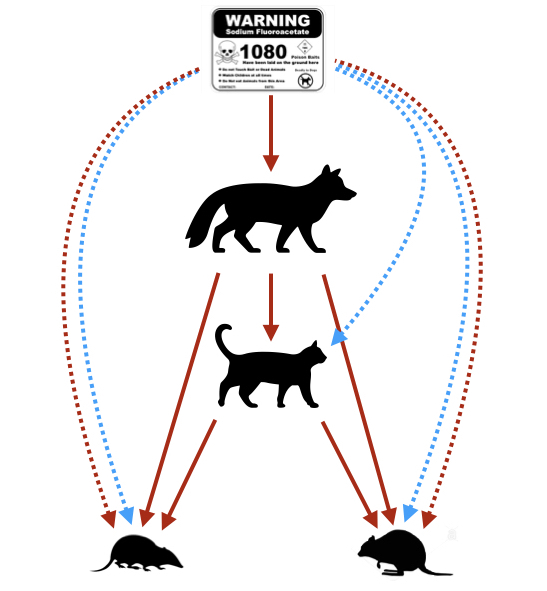
\includegraphics[width=0.7\linewidth]{figure/conceptual_diagram} 

}

\caption{Conceptual diagram of direct (solid line) and indirect (dashed line) positive (blue) and negative (red) interactions investigated in this thesis. Fox control in Australia (in this case via 1080 poison-baiting) aims to suppress invasive red foxes, thereby benefiting two threatened prey species such as the southern brown bandicoot and long-nosed potoroo. However, fox control may cause mesopredator release of feral cats (because foxes may exert top-down and competitive pressure on cats), which could lead to a net negative impact on their shared prey such as these two threatened native mammals.}\label{fig:intro-conceptual}
\end{figure}
\hypertarget{otways17}{%
\chapter{Unexpectedly high densities of feral cats in a rugged temperate forest}\label{otways17}}

\hypertarget{abstract}{%
\section*{Abstract}\label{abstract}}
\addcontentsline{toc}{section}{Abstract}

Effective invasive predator management requires accurate knowledge of population density. However, density can be difficult to estimate for wide-ranging, cryptic and trap-shy species, such as the feral cat \emph{Felis catus}. Consequently, few density estimates exist for this invasive predator of global significance, particularly from rugged, mesic or structurally complex habitats where detection is challenging. In this study, we estimated feral cat density in the wet forests and cool temperate rainforests of the Otway Ranges, south-eastern Australia, to (1) provide a density estimate for this rarely surveyed habitat type, and (2) verify predictions from a continental-scale model of feral cat density. We deployed 140 camera traps across two independent 49 km\textsuperscript{2} grids and identified individual feral cats based on unique pelage markings. Using spatially explicit mark-resight models, we estimated that there were 1.14 cats km\textsuperscript{-2} (95\% CI: 0.88 -- 1.47). This is more than three times the average cat density in natural environments across Australia, and at least five times higher than model-based predictions for the Otway Ranges. Such high densities of feral cats likely reflect the abundance of small native mammals and lack of apex predators in our study area. Our findings contradict the widespread assumption that feral cats occur at very low densities in mesic and rugged habitats. Underestimating the density of feral cats in these environments has significant implications for pest animal management and biodiversity conservation.

\newpage

\hypertarget{introduction}{%
\section{Introduction}\label{introduction}}

Accurate estimates of the distribution and abundance of invasive predators are essential to determine ecosystem impacts, inform effective management and target control efforts. However, this information is difficult to obtain as predators are often cryptic, trap-shy and occur at low densities (Royle, Stanley, \& Lukacs 2008). A prominent example is the feral cat \emph{Felis catus}, which is implicated in the extinction or decline of 430 species globally (Doherty \emph{et al.} 2017). A better understanding of feral cat density has been highlighted as a priority for effective management of both this species and its threatened native prey (Woinarski, Burbidge, \& Harrison 2014; Legge \emph{et al.} 2017; Moseby \emph{et al.} 2019).

Legge \emph{et al.} (2017) developed a continental-scale model of feral cat density for Australia which has had considerable implications for feral cat research and management. For instance, the model has been used to estimate the number of birds, reptiles and mammals killed annually across Australia by feral cats (Woinarski \emph{et al.} 2017; Woinarski \emph{et al.} 2018; Murphy \emph{et al.} 2019). As the model estimated that there were considerably fewer feral cats in Australia than previously expected, it also casts doubt on the feasibility of Australian Federal Government's plan to cull two million feral cats between 2015 and 2020 (Doherty \emph{et al.} 2019). Given the importance of feral cat density estimates for policy, planning and management, it is vital to verify and refine the model's predictions.

The underlying data used by Legge \emph{et al.} (2017) had several limitations, including that feral cat density estimates were not available for any wetland, mangrove, dense heath or rainforest environments in Australia (Legge \emph{et al.} 2017). This likely reflects the difficulty of access and ineffectiveness of traditional feral cat monitoring methods (track counts and spotlight counts) in these structurally complex habitats (Denny \& Dickman 2010). Legge \emph{et al.} (2017) highlighted the need for more site-based density surveys, particularly in these under-studied environments. Further, nearly all of the density estimates collated by Legge \emph{et al.} (2017) were based on studies that did not identify individual cats or account for imperfect detection (i.e.~the possibility that some individuals were not detected). Such methods can be unreliable when inferring across sites, times, ecological contexts and different detection methods (Edwards \emph{et al.} 2000; Hayward \emph{et al.} 2015), particularly for species such as cats whose densities may fluctuate substantially over time in some regions (Legge \emph{et al.} 2017). Concurrent surveys of cats on Kangaroo Island and the adjacent Australian mainland suggests that the Legge \emph{et al.} (2017) model may substantially underestimate this variation in density (Taggart \emph{et al.} 2019).

Robust population density estimates for cryptic and wide-ranging species based on individual identification are now more feasible due to recent advances in technology and statistical models. Camera-traps that sense temperature-in-motion provide an efficient survey approach across diverse environments and are particularly beneficial for studies of trap-shy species with unique markings, such as feral cats (Bengsen, Butler, \& Masters 2011). Concurrently, spatial mark-resight (SMR) models, an extension of spatial capture-recapture models, enable population density estimates when a portion of the population can be individually identified (Royle \emph{et al.} 2013). These models consider both the distribution and movement of individuals across the landscape in relation to the placement of detectors, and account for imperfect detection (Gardner, Royle, \& Wegan 2009). The combination of camera-trap surveys to identify individuals and spatial capture-recapture methods to estimate density has shown promise for both feral and domestic cats (McGregor \emph{et al.} 2015b; Jiménez \emph{et al.} 2017; Robley \emph{et al.} 2017; Cove \emph{et al.} 2018; Robley, Ramsey, \& Woodford 2018).

The small number of studies that have estimated feral cat density in the mesic regions of south-eastern Australia indicate that these habitats support few feral cats relative to other regions (Legge \emph{et al.} 2017). However, survey effort for feral cats in these environments has been low compared to more arid regions. Our study therefore aimed to provide: (1) a density estimate for a rarely surveyed environment -- a matrix of wet forest and cool temperate rainforest, and (2) an independent verification of the prediction from the Legge \emph{et al.} (2017) continental-scale model of feral cat density for the Otway region. To achieve these aims, we undertook a camera-trap survey over 8,230 trap nights at 140 sites in the Otway Ranges, south-eastern Australia. We derived feral cat density estimates by applying SMR analysis to our camera survey data. In line with the Legge \emph{et al.} (2017) model which estimates 0.17 - 0.23 cats km\textsuperscript{-2} for this study region, we predicted cat density here would be slightly below the average cat density in Australian `natural areas' (0.27 cats km\textsuperscript{-2}, Legge \emph{et al.} 2017).

\newpage

\hypertarget{methods}{%
\section{Methods}\label{methods}}

\hypertarget{study-area}{%
\subsection{Study area}\label{study-area}}

Our study was conducted in the Great Otway National Park and Otway Forest Park, Victoria, Australia (38.42 °S, 142.24 °E). The locality is 90 -- 440 m above sea level. and has a cool-temperate climate: maximum daily temperatures average 19.3 °C in summer and 9.5 °C in winter; annual rainfall averages 1955 mm (Bureau of Meteorology 2021). The vegetation is a mosaic of old-growth shrubby wet forest, wet forest and cool temperate rainforest, with an overstorey of tall eucalyptus spp. (primarily \emph{Eucalyptus regnans}), \emph{Acacia melanoxylon} and \emph{Nothofagus cunninghamii}, and a midstorey dominated by tree ferns, \emph{Acacia verticillata}, \emph{Pomaderris aspera} and \emph{Olearia argophylla}. The understorey predominantly comprises a dense layer of ferns and graminoids, but is relatively open in steep gullies. The terrestrial predator guild is depauperate, with the introduced red fox \emph{Vulpes vulpes} being the only other significant competitor of feral cats. Our camera survey and other live-trapping surveys indicate an abundance of small native mammals within the study region, particularly native rats and antechinus (Banikos 2018).

\hypertarget{study-design}{%
\subsection{Study design}\label{study-design}}

We deployed camera traps in two grids, each approximately 49 km\textsuperscript{2} and separated by more than five kilometres (Fig. \ref{fig:otways17-map}). The northern grid comprised 67 survey sites, spaced an average of 526 m apart (86 -- 848 m). The southern grid comprised 73 survey sites, spaced an average of 547 m apart (352 -- 719 m). We deployed a Reconyx Hyperfire HC600 survey camera, with infrared flash and temperature-in-motion detector (Reconyx, Holmen, Wisconsin), at each site. Sites were located at least 30 m away from roads and tracks, as we sought to estimate cat density in `natural areas' where native prey occurs (and reduce the possibility of camera theft). Cameras functioned for 37 -- 68 days (mean 59) from 26 June to 2 September 2017, totalling 8230 trap nights. Each camera was placed on a tree approximately 30 cm above the ground and faced towards a lure 2 -- 2.5 m away. Vegetation in the camera's line of sight was cleared to prevent false triggers. The lure comprised an oil-absorbing cloth doused in tuna oil and placed inside a PVC pipe container with a mesh top. Ten to 30 small white feathers were also attached to the outside of the PVC pipe container. Each lure was fastened near the top of a one-metre wooden stake. Cameras took five immediately consecutive photographs when triggered, with no quiet period between trigger events.

\hypertarget{individual-cat-identification}{%
\subsection{Individual cat identification}\label{individual-cat-identification}}

Images of feral cats were first grouped as marked or unmarked (black) individuals. Although some black cats had small white neck/chest coat splotches, these were not always visible (cats often moved with their heads down), and so all black cats were considered unmarked to avoid double-counting. The marked portion were tabby cats with naturally unique coat markings. These were further classified into distinct groups: stripes \& spots, thick swirls, other markings (ginger, distinctive breeds etc.) and unknown (due to poor image quality). At least two independent observers identified individual cats from these groups based on matches in unique markings, predominantly on the front legs, torso and across both flanks. Observers collated folders of images of unique individuals for reference. Discrepancies between observers were reviewed together until consensus was reached. If no consensus was reached, the marked cat was considered unidentifiable.

\hypertarget{estimating-population-density}{%
\subsection{Estimating population density}\label{estimating-population-density}}

We used conventional SMR models for an unknown number of marked individuals (sighting-only) to estimate feral cat density. These models assume that uniquely marked cats are a random sample of the population, with the same movement ecology as unmarked cats. We fitted models using the `secr' R-package (v. 3.2.1, Efford 2021) in R (v. 3.5.2, R Core Team 2020), as per Efford \& Hunter (2018).

Capture histories were collapsed into 24-h occasions, beginning at midday each day (as this was the time of day with the lowest observed cat activity). We used a 3500 m buffer around the outermost coordinates of the trapping grids to ensure density was estimated over an area large enough to include the activity centres of all cats potentially exposed to our survey (Royle \emph{et al.} 2013); this distance is larger than the estimated average maximum width of home ranges of large, male cats close to this region (n = 3; B.A. Hradsky, unpublished data).

In SMR models, detectability is defined by two parameters: \emph{g}\textsubscript{0}, the probability of detecting an animal (per occasion) if a detector was to be placed in the part of its home range where most time is spent, and sigma, a spatial scale parameter relating to home range size. Animals are assumed to have approximately circular home ranges, with the probability of detection declining with distance from the home range centre. We tested three shapes of this decline in detection probability: half‐normal, hazard‐rate, and exponential, and used the detector function with the lowest Akaike's Information Criterion adjusted for small sample size (`AICc', Burnham \& Anderson 2004) for subsequent model fitting.

As the lures may have decreased in potency over the sampling session, we tested for a linear trend in \emph{g}\textsubscript{0} over time. We also tested whether density differed between the two grids, with and without a linear time trend. We compared these models to the null model (where detection and density were kept constant across both grids) using AICc. Overdispersal in the unmarked sightings was adjusted for as per Efford \& Hunter (2018) and a spatial resolution of 0.6 of the sigma estimate was used for all models (Efford 2021).

\newpage

\(~\)

\(~\)

\(~\)
\begin{figure}

\hfill{}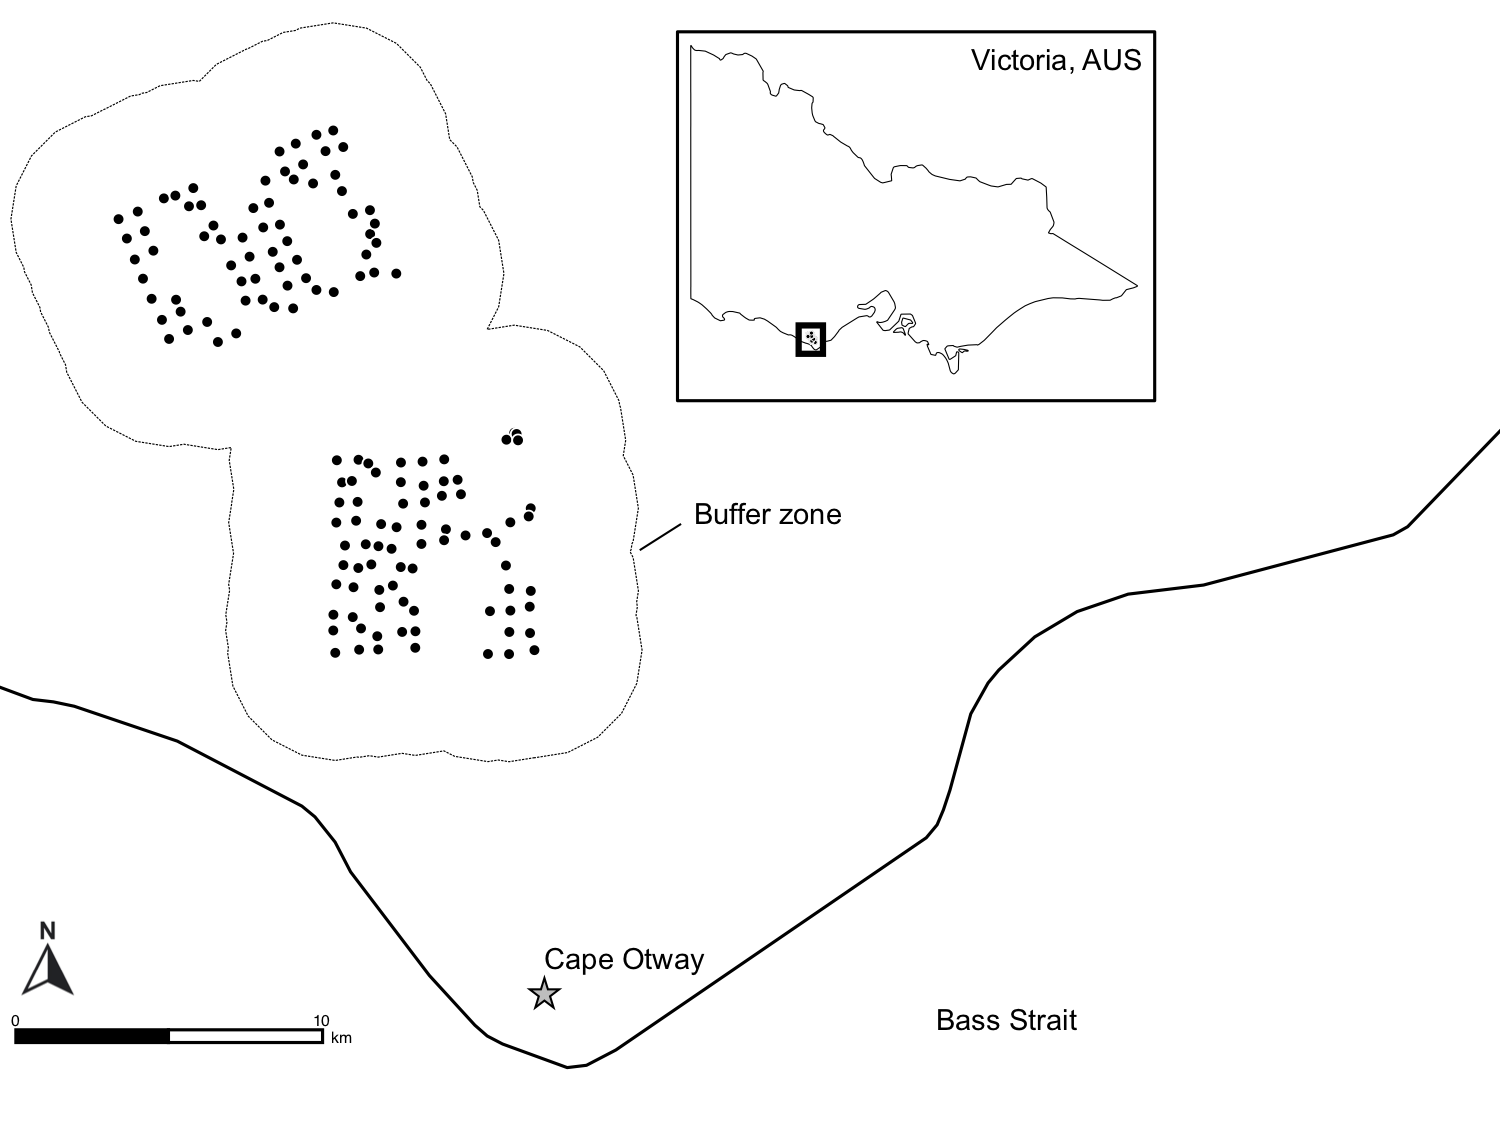
\includegraphics[width=1\linewidth]{figure/otways17_map} 

\caption{Study area, western Otway Ranges, Victoria, Australia, showing the location of the camera-trapping sites (black dots) within the 3500 m buffer zone (thin grey line). The holes in the camera-trapping grids occurred due to rugged topography and limited access to these areas.}\label{fig:otways17-map}
\end{figure}
\newpage

\hypertarget{results}{%
\section{Results}\label{results}}

We detected feral cats at 55\% of sites. Of these detections (1 detection = one or more visits of an individual/unidentifiable/unmarked cat to a camera-trap per 24-h occasion), 41\% were unmarked (black) cats. Of the marked cat detections, 89\% could be reliably identified to the individual-level -- 47 individuals were identified. The number of detections, number of identified individuals and mean distances moved were similar across the two camera-trapping grids (Table \ref{tab:otways17-stats}).

The top-ranked model estimated a density of 1.14 cats km\textsuperscript{-2} (95\% CI: 0.88 -- 1.47), with no difference in density between grids but a linear decrease in \emph{g}\textsubscript{0} over time (5.7\% decrease per week; Fig. \ref{fig:otways17-g0t}; Table \ref{tab:otways17-stats}). The second-ranked model (dAICc 1.74, Akaike weight 0.23) indicated that densities were slightly higher at the northern than southern grid, although confidence intervals overlapped substantially (Table \ref{tab:otways17-estimates}). The hazard-rate detector function best described the rate at which detection probability changed with the distance of the camera from the centre of a cat's home range (Table \ref{tab:otways17-detfn}). Estimates of feral cat density were robust to all model specifications, with the mean estimate varying by less than 0.2 cats km\textsuperscript{-2} between all models (Table \ref{tab:otways17-stats}).

\newpage

\(~\)

\(~\)

\(~\)

\begingroup\fontsize{10}{12}\selectfont
\begin{longtable}[t]{lrrr}
\caption{\label{tab:otways17-stats}Summary of raw camera survey data for feral cats in the Otway Ranges, Victoria, Australia, 2017.}\\
\toprule
Summary statistic & southern grid & northern grid & both grids\\
\midrule
\endfirsthead
\caption[]{\label{tab:otways17-stats}Summary of raw camera survey data for feral cats in the Otway Ranges, Victoria, Australia, 2017. \textit{(continued)}}\\
\toprule
Summary statistic & southern grid & northern grid & both grids\\
\midrule
\endhead

\endfoot
\bottomrule
\endlastfoot
Number of camera sites & 73 & 67 & 140\\
Sites where cats detected (\%) & 51 & 62 & 55\\
Number of unmarked detection events & 47 & 48 & 95\\
Number of identifiable, marked detection events & 60 & 59 & 119\\
Number of unidentifiable, marked detection events & 10 & 5 & 15\\
\addlinespace
Total number of identified individuals & 23 & 24 & 47\\
Number of cats resighted at different cameras & 8 & 6 & 14\\
Mean recapture distance (m) & 653 & 774 & 716\\
Maximum recapture distance (m) & 905 & 1701 & 1701\\*
\end{longtable}
\endgroup{}

\newpage

\(~\)

\(~\)

\(~\)
\begin{longtable}[t]{lllllllrrr}
\caption{\label{tab:otways17-estimates}Comparison of spatial mark-resight models and density estimates}\\
\toprule
\multicolumn{2}{c}{Model} & \multicolumn{4}{c}{Model comparison} & \multicolumn{4}{c}{Density estimate (cats km-2)} \\
\cmidrule(l{3pt}r{3pt}){1-2} \cmidrule(l{3pt}r{3pt}){3-6} \cmidrule(l{3pt}r{3pt}){7-10}
Density & g0 & K & AICc & dAICc & AICcwt & grid & estimate & lcl & ucl\\
\midrule
\endfirsthead
\caption[]{\label{tab:otways17-estimates}Comparison of spatial mark-resight models and density estimates \textit{(continued)}}\\
\toprule
\multicolumn{2}{c}{Model} & \multicolumn{4}{c}{Model comparison} & \multicolumn{4}{c}{Density estimate (cats km-2)} \\
\cmidrule(l{3pt}r{3pt}){1-2} \cmidrule(l{3pt}r{3pt}){3-6} \cmidrule(l{3pt}r{3pt}){7-10}
Density & g0 & K & AICc & dAICc & AICcwt & grid & estimate & lcl & ucl\\
\midrule
\endhead

\endfoot
\bottomrule
\endlastfoot
1 & T & 5 & 1568.84 & 0 & 0.71 & both & 1.14 & 0.88 & 1.47\\
grid & T & 6 & 1570.68 & 1.84 & 0.28 & north & 1.23 & 0.90 & 1.68\\
 &  &  &  &  &  & south & 1.05 & 0.78 & 1.42\\
1 & 1 & 4 & 1578.37 & 9.53 & 0.01 & both & 1.14 & 0.89 & 1.48\\
grid & 1 & 5 & 1579.66 & 10.82 & 0 & north & 1.25 & 0.91 & 1.72\\
\addlinespace
 &  &  &  &  &  & south & 1.04 & 0.77 & 1.40\\*
\end{longtable}
\emph{T = linear time trend}

\emph{K = number of parameters estimated}

\emph{AICc = Akaike's Information Criterion with small-sample adjustment}

\emph{dAICc = difference between AICc of this model and the model with smallest AICc}

\emph{AICcwt = AICc model weight}

\emph{lcl -- lower 95\% confidence limit}

\emph{ucl -- upper 95\% confidence limit}

\newpage

\hypertarget{discussion}{%
\section{Discussion}\label{discussion}}

Our work provides one of the first robust estimates of feral cat density for a temperate wet forest in Australia. Our estimate of 1.14 cats km\textsuperscript{-2} (95\% CI: 0.88 -- 1.47) is five times higher than that predicted by the Legge \emph{et al.} (2017) model for this location (0.17 - 0.23 cats km\textsuperscript{-2}), and more than three times higher than the predicted continental mean density for feral cats in `natural areas' (0.27 cats km\textsuperscript{-2}, Legge \emph{et al.} 2017). The mesic coastal areas of Australia were previously thought to support the lowest densities of feral cats across the continent, particularly rugged and wet regions, such as rainforests (Dickman 1996; Johnson 2006; Legge \emph{et al.} 2017; McDonald \emph{et al.} 2017). Accordingly, feral cats were believed to have relatively less impact on native species in these environments (Burbidge \& Manly 2002; Doherty \emph{et al.} 2017; Woinarski \emph{et al.} 2017; Radford \emph{et al.} 2018; Woinarski \emph{et al.} 2018; Murphy \emph{et al.} 2019). Our finding is therefore startling, and prompts a rethink about the threat that feral cats may pose to native fauna in mesic habitats.

The high density of feral cats in our study region likely reflects the high productivity of the landscape and abundant populations of some prey species. Our study region has the highest annual rainfall in Victoria (Bureau of Meteorology 2021), and live-trapping surveys in our study site show consistent, near saturation of small mammal traps, predominantly bush rats \emph{Rattus fuscipes} and \emph{Antechinus spp}. (Z. Banïkos, unpublished data). Several images from our study confirmed that feral cats prey upon these taxa. These small mammals may be relatively robust to introduced predators due to their high fecundity and generalist habitat requirements (e.g., Banks 1999). However, by supporting high densities of feral cats, they may also facilitate high levels of predation on rarer and more vulnerable species (Smith \& Quin 1996), such as the now locally extinct smoky mouse \emph{Pseudomys fumeus} (Menkhorst \& Broome 2006). Significant declines and local extinctions of other small mammals have also been reported across the eastern Otways (Wayne, Wilson, \& Woinarski 2017). Understanding temporal trends in these predator-prey dynamics and the relationships between introduced predators and their native primary and alternative prey is a key priority for future research.

The lack of apex predators and competitors in the Otway Ranges may also facilitate high feral cat densities. Dingoes \emph{Canis familiaris}---higher order predators (Johnson, Isaac, \& Fisher 2007)---and tiger quolls \emph{Dasyurus maculatus}---key competitors (Glen \& Dickman 2005)---are functionally extinct in the Otway Ranges. We detected foxes at 25\% of sites (M. Rees, unpublished data) but the extent to which foxes exert top-down control on feral cats is unclear. Changes in feral cat abundance, behaviour and/or diet have been observed in response to fox control (Molsher \emph{et al.} 2017; Hunter \emph{et al.} 2018), and the relationship could be further clarified using robust density estimates under experimental manipulations of fox density.

The belief that feral cat densities in Australia are lower in mesic forests than open habitats stems partly from the lack of robust density estimates from forests, and partly from observations that cats have greater hunting success and are more detectable in open microhabitats (McGregor \emph{et al.} 2014, 2015b; Hohnen \emph{et al.} 2016; McDonald \emph{et al.} 2017) and select for savannah over rainforest (McGregor, Cliff, \& Kanowski 2017). However, the variation in understorey structure (from extremely dense to relatively open) in our study region potentially creates ideal shelter and foraging habitat for feral cats, which often hunt along edges between dense and open vegetation (Doherty, Bengsen, \& Davis 2015). Our findings challenge the belief that cat density is low in mesic forests, and instead concur with the global pattern that feral cats have smaller, overlapping home ranges in productive, low-seasonal environments, resulting in higher population densities (Bengsen \emph{et al.} 2016).

Our surveys clearly need replicating in other mesic environments before they can be generalised. Nonetheless, higher than expected densities of feral cats in mesic and complex environments would have serious implications for biodiversity conservation. Feral cats are thought to be a key driver of the recent declines of critical-weight-range mammals in northern Australia (Woinarski \emph{et al.} 2010; Fisher \emph{et al.} 2014; Davies \emph{et al.} 2018). Contemporary mammal declines are also occurring in temperate Australia, including the Otway Ranges (Bilney, Cooke, \& White 2010; Wayne \emph{et al.} 2017; Lindenmayer \emph{et al.} 2018). A better understanding of feral cat densities in these regions is essential for identifying key threatening processes and improving management outcomes.

In conclusion, our study shows that feral cats can occur at high densities in wet forests and cool temperate rainforests, contrary to previous expectations. Further research is needed to understand the impacts of this on native mammal populations, and the mechanisms that drive spatial variation in feral cat density, including the influence of habitat type, productivity, disturbance events and interactions with other predators. New spatial capture-recapture methods will likely play a powerful role in improving understanding of the ecology of this globally-significant predator. Our work provides a strong foundation for future investigations, as our methodology allows for robust evaluations of feral cat density, particularly under experimental manipulations and population comparisons.

\hypertarget{occ}{%
\chapter{Fox control and fire influence the occurrence of invasive predators and threatened native prey}\label{occ}}

\hypertarget{abstract-1}{%
\section*{Abstract}\label{abstract-1}}
\addcontentsline{toc}{section}{Abstract}

It is challenging to disentangle management impacts from other population drivers, including `natural' processes and co-occurring threats. However, this is particularly important when management may have unintended consequences, such as mesopredator release following top predator control or increased vulnerability to predation following prescribed fire.

We explored the effects of long-term, broadscale poison-baiting programs on the distribution of red foxes \emph{Vulpes vulpes} (targeted invasive predator), feral cats \emph{Felis catus} (unmanaged invasive competitor) and two of their threatened native prey, in heterogenous, fire-affected landscapes of south-eastern Australia. We synthesised data from 3,667 camera-trap deployments across 1,232 sites (172,052 trap-nights). Our inference was strengthened by spatial replication of fox control treatments, within and across two large regions, the inclusion of experimental manipulations and space-for-time designs, and the repeat sampling of sites for up to 7 years.

Fox control effectiveness---in terms of decreased probability of fox occurrence and increased probability of prey occurrence---depended on the duration and intensity of the poison-baiting programs. However, the strength of these effects was inconsistent across the two native prey species; fox control was strongly beneficial to the long-nosed potoroo \emph{Potorous tridactylus} but had no effect on southern brown bandicoot \emph{Isoodon obesulus} occurrence. Cat occupancy tended to be higher in landscapes with long-term fox control, although we found no effect of fox-bait density on fine-scale cat occurrence. Time since fire (0 -- 80 years) was associated with the occurrence of each study species, but its association with invasive predators also differed between vegetation types.

Invasive predators and altered fire regimes are key, often overlapping biodiversity threats, however, other landscape contexts such as vegetation type and ruggedness are also important drivers of mammal distributions. Our work highlights the importance of fine-scale monitoring and consideration of multiple drivers in distribution models to develop effective, tailored conservation strategies.

\newpage

\hypertarget{introduction-1}{%
\section{Introduction}\label{introduction-1}}

Accurate and precise estimates of the effects of management are essential to inform conservation decision-making, ensure cost-effective allocation of resources and to help identify potential unintended consequences of interventions (Christie \emph{et al.} 2020). However, reliable inference about the effects of landscape-scale management, including identifying the cause of nil or perverse outcomes, is often difficult to achieve because target populations fluctuate naturally and are often subject to multiple co-occurring threats and management actions (Pressey \emph{et al.} 2007; Sugihara \emph{et al.} 2012). Separating management effects from other drivers is particularly difficult for species that occur patchily across broad distributions (Tulloch \emph{et al.} 2016).

Invasive predator management is a classic example of these challenges. Predators can have devastating impacts on native biodiversity when introduced beyond their native range, and so invasive predators are often lethally controlled (Sih \emph{et al.} 2010; Bellard, Genovesi, \& Jeschke 2016; Doherty \emph{et al.} 2016). Quantifying the degree of invasive predator suppression, the responses of their native prey and any unintended outcomes across gradients of predator control is key to designing cost-effective management programs (Baxter \emph{et al.} 2008; Walsh \emph{et al.} 2012; Cattarino \emph{et al.} 2016). However, the ability of associated monitoring programs to detect these signals is often confounded by co-occurring threats, management actions and natural drivers. This is concerning because, few or even negative effects on native biodiversity are commonly observed following invasive predator control, particularly when multiple introduced species are present (Ballari, Kuebbing, \& Nuñez 2016).

There are several explanations for why native prey species may not benefit from invasive predator control. Firstly, control efforts may not sufficiently reduce the density of invasive predators---predators can be remarkably resilient to low-effort culling (Lieury \emph{et al.} 2015; Moseby \emph{et al.} 2019). Secondly, invasive predator suppression may lead to a `release' of a subordinate predator (referred to as the `mesopredator release hypothesis', Crooks \& Soulé 1999) or competitor species (Ruscoe \emph{et al.} 2011), which could potentially worsen net outcomes for native species (Doherty \& Ritchie 2017). Thirdly, predation by introduced species may not be the primary limit on native prey populations (Banks 1999). Hence, quantifying the degree of apex predator suppression and testing the mesopredator release hypothesis (Crooks \& Soulé 1999), are important steps toward understanding prey responses to lethal predator control and identifying the cause of a nil response, if observed (Salo \emph{et al.} 2010).

Quantifying the impacts of planned fire on fauna is similarly complex. Fire can drive the persistence and abundance of fauna populations, primarily through its effects of vegetation structure (Monamy \& Fox 2000). As these effects persist for decades or centuries, are nonlinear, and vary across environmental conditions (Haslem \emph{et al.} 2011), fauna species' responses to fire often vary across heterogeneous landscapes (Nimmo \emph{et al.} 2014; Swan \emph{et al.} 2015). Predicting the long-term ramifications of fire for predators and prey is a key challenge for managers who are tasked with stemming the decline of native fauna populations while simultaneously managing fuel loads to protect against the increasing threat of large wildfires (Clarke 2008; Hradsky 2020).

These separate challenges are amplified in contexts where invasive predators occur in fire-prone landscapes (Doherty \emph{et al.} 2015b). Nonetheless, disentangling the complex and potentially interacting effects of invasive predator and fire management on threatened native fauna is crucial for effective native mammal conservation in Australia, which has experienced some of the worst biodiversity declines in recent world history (Waldron \emph{et al.} 2017; Woinarski \emph{et al.} 2019). Predation by introduced species and altered fire regimes are primary drivers of these declines (Woinarski, Burbidge, \& Harrison 2015), but other threatening processes such as habitat fragmentation, and natural drivers such as vegetation type and rainfall dynamics also play an important role in shaping contemporary native mammal distributions (May \& Norton 1996; Hale \emph{et al.} 2016). Lethal control (primarily using 1080 poison-baiting) of the introduced red fox \emph{Vulpes vulpes} (hereafter `fox') and prescribed burning (primarily for asset protection) are among the most common management actions in protected areas, however, we have a poor understanding of their effects on native fauna (Clarke 2008; McLeod \emph{et al.} 2008; Braysher 2017; Lindenmayer \emph{et al.} 2018). This is partly because there is strong spatial overlap of these threats and management actions (Evans \emph{et al.} 2011) and potential unintended consequences often go unmeasured.

Feral cats Felis catus (hereafter `cat') are one of the most widespread and damaging invasive vertebrates (Medina \emph{et al.} 2011; Doherty \emph{et al.} 2016; Legge \emph{et al.} 2020). Cat populations are extremely difficult to suppress lethally, and so there is concern around management actions which may inadvertently increase cat impacts on native prey, particularly fox control (Fisher \emph{et al.} 2015; Lazenby, Mooney, \& Dickman 2015; Doherty \& Ritchie 2017). In southern Australian regions where native apex predators have been extirpated, foxes are the largest terrestrial predators and are expected be filling the role of an apex predator by potentially suppressing smaller-sized cats through both aggressive and competitive top-down effects (Wayne \emph{et al.} 2017). Fox control could therefore cause mesopredator release of cats, but quantitative evidence is conflicted (even within landscape spatial replicates of studies, Davey \emph{et al.} 2006) and a recent meta-analysis found little statistical evidence overall (Hunter \emph{et al.} 2018).

One possible reason for this conflicting inference is that predator removal studies are typically conducted and analysed across broad regions. Yet invasive predator show strong habitat selection preferences at fine spatial scales (Hradsky \emph{et al.} 2017c; McGregor, Cliff, \& Kanowski 2017). In particular, both foxes and cats are expected to move into and increase their use of recently burnt areas, capitalising on vulnerable prey lacking understorey shelter (although it is unclear how long this effect lasts for, Hradsky 2020). Accounting for differences in preferences for fine-scale landscape features, as well as the effects of other management actions, may improve our understanding of predator control outcomes, including potential invasive mesopredator release.

In this study, we assessed the effect of landscape-scale lethal fox management in two protected, fire-prone conservation regions of south-eastern Australia: the Glenelg region and Otway Ranges. We quantified the effects of fox management on the occupancy of foxes (the managed species), cats (unmanaged competitor), and two threatened species (important prey species of both predators) that are the primary focus of the conservation programs: the southern brown bandicoot \emph{Isoodon obesulus} (hereafter `SBB') and long-nosed potoroo \emph{Potorous tridactylus} (hereafter `LNP'). Our study dataset combined experimental and space-for-time approaches through one-off and repeat deployments of 3,667 camera-traps across 1,232 sites over a period of seven years. In the Glenelg region, foxes had been continuously controlled for 8 - 14 years (at the time of these surveys); In the Otway region, we examined the effects of a new fox control program over a 3-year period; both regions also included substantial unbaited areas serving as experimental controls. Occupancy-detection models (MacKenzie \emph{et al.} 2002) were first used to investigate the detectability of each species. As detectability was generally high, we used Generalised Additive Models (hereafter `GAMs', Wood 2017) to explore the potentially nonlinear responses of each species to fox control effort (1080 poison-bait density), time since fire (0 - 80 years) across vegetation types, and other environmental drivers (elevation, terrain ruggedness, recent rainfall, topographic wetness and habitat fragmentation). The GAMs did not account for imperfect detection but allowed nonlinear responses and more complex model structures.

We predicted that the density of poison fox-baits would be negatively associated with the probability of fox occurrence and, consequently, also positively associated with cat occurrence (in line with the mesopredator release hypothesis). We also predicted that these effects would be stronger be stronger in the Glenelg region where fox control has occurred over a longer period and baits are replaced more frequently than in the Otway Ranges region. Based on previous studies within the Glenelg region (Robley \emph{et al.} 2014), and more broadly across Australia (Hunter \emph{et al.} 2018), we expected SBB and LNP occupancy to be positively associated with fox-bait density. We expected species-specific responses to environmental drivers. We predicted that both predators would be more likely to occupy recently and frequently burnt areas (Hradsky 2020), and conversely that long unburnt vegetation would support a high prey occupancy. Finally, we expected some variations in responses to fire across vegetation types, due to differences in post-fire vegetation regrowth rates (Swan \emph{et al.} 2015).

\newpage

\hypertarget{methods-1}{%
\section{Methods}\label{methods-1}}

\hypertarget{study-regions}{%
\subsection{Study regions}\label{study-regions}}

We compiled data from multiple camera-trap studies across two regions in south-west Victoria, Australia: the Glenelg region and Otway Ranges (Fig. \ref{fig:occ-map}). Introduced foxes and cats are the only medium-large functional mammalian terrestrial carnivores here: native dingoes \emph{Canis familiaris} are long-absent throughout, while spot-tailed quolls \emph{Dasyurus maculatus} are long-absent in the Glenelg region and likely functionally extinct in the Otway Ranges (last confirmed sighting in 2014). Managers frequently implement prescribed fire across both regions, primarily to reduce fuel loads.

\hypertarget{glenelg-region}{%
\subsubsection{Glenelg region}\label{glenelg-region}}

In the Glenelg region (38°05'54''S 141°44'41''E), large patches of natural vegetation are fragmented mostly by pastoral farming and residential properties (Fig. \ref{fig:occ-map}). Here, the primary vegetation communities are heathy woodland, lowland forest, herb-rich woodland and wet heathland (Department of Environment, Land, Water \& Planning 2020a). The Glenelg region has an annual mean minimum temperature of 8.1 °C in winter, and 20.0 °C in Summer (Bureau of Meteorology 2021). Mean annual rainfall averages 835 mm (Bureau of Meteorology 2021). Terrain is gently undulating in the Glenelg region; study sites ranged from 12 - 180 m above sea level.

\hypertarget{otway-ranges}{%
\subsubsection{Otway Ranges}\label{otway-ranges}}

The Otway Ranges (38°57'82''S 141°68'41''E) is a largely continuous patch of natural vegetation with a strong east-west rainfall gradient (Fig. \ref{fig:occ-map}). A matrix of cool temperate rainforest and wet forest at high-altitudes in the south-west descend into a large heathland directly north, and into dry forests and then heathlands to the north-east. Annual rainfall averages 1955 mm in the southwest, dropping to 627 mm in the eastern Otways (Bureau of Meteorology 2021). Mean minimum temperatures in the Otway Ranges are 8° in winter and 13° in summer (Bureau of Meteorology 2021). Our study sites ranged from 23 - 617 m above sea level.

\hypertarget{fox-control-and-monitoring}{%
\subsection{Fox control and monitoring}\label{fox-control-and-monitoring}}

In broad sections of each region, government land managers conduct ongoing targeted lethal fox control for biodiversity conservation. Poison-baits containing 3 mg of sodium fluroacetate (compound 1080) are buried at a depth of 12 - 15 cm at 1-km intervals along accessible forest tracks and roads. Different road densities therefore result in spatially variable densities of poison-baits.

\hypertarget{glenelg-region-1}{%
\subsubsection{Glenelg region}\label{glenelg-region-1}}

In the Glenelg region, three distinct forest blocks have been subject to poison-baiting since October 2005, with fortnightly bait replacements. These forest blocks, along with three similar, unbaited forest blocks to the north are simultaneously surveyed annually under the `Glenelg Ark' fox control program (40 camera-sites per block, Robley \emph{et al.} 2020). Hair-tubes were used to monitor small prey species from 2005 - 2013 (presented in Robley \emph{et al.} 2014), replaced by camera-traps from 2013 onwards (here we present camera-trap data from 2013 - 2019, Robley \emph{et al.} 2020). We also included a further 425 camera-trap deployments at unique locations from early 2018 (M.W.R., PhD surveys). This totals 2,041 camera-trap deployments in the Glenelg region, collected in a control-impact experimental design (foxes had been continuously controlled for at 8 - 14 years in the treatment landscapes by the time of these surveys).

\hypertarget{otway-ranges-1}{%
\subsubsection{Otway Ranges}\label{otway-ranges-1}}

Fox-baiting commenced in small sections of the Otway Ranges in 2008 and large-scale systematic baiting began in 2016 - 2017 under the `Otway Ark' program (Robley, Moloney, \& Parks Victoria West Coast District Team 2019). For the first six weeks of the Otway Ark program, poison-baits were replaced weekly, this then changed to ongoing monthly bait-replacement. There was a pause in baiting for approximately six months during the second half of 2018. Fox control recommenced in late 2018 with four weeks of fortnightly bait-replacement, before returning to monthly bait-replacement. A large section of the Otway Ranges to the north-west remains unbaited as it is a known stronghold for native prey species, and so the need for fox control was not justified (but remains monitored as part of the Otway Ark program, Robley, Moloney, \& Parks Victoria West Coast District Team 2019). Otway Ark managers survey 372 camera-trap sites annually (sequentially across the region); we present one `before' baiting survey and two `after' baiting surveys of each site from 2016 - 2018, totalling 1,113 camera-trap deployments (Robley, Moloney, \& Parks Victoria West Coast District Team 2019). We also include data from an additional before-after control-impact surveys (one `before' baiting survey and two `after' bating surveys) in the western section of the Otway Ranges, conducted annually 2017 - 2019 (M.W.R PhD surveys). This added a further 195 sites and 524 camera-trap deployments.

\hypertarget{camera-trap-set-ups}{%
\subsubsection{Camera-trap set-ups}\label{camera-trap-set-ups}}

All camera-trap deployments consisted of a Reconyx (Holmen, Wisconsin) brand camera-trap (white or infrared flash), attached to a tree or a metal picket, facing a lure. The Glenelg Ark and Otway Ark fox monitoring programs positioned camera-traps at least 40 cm above ground on a tree or a metal picket, angled downwards toward a lure approximately 1 - 1.5 m away (Robley, Moloney, \& Parks Victoria West Coast District Team 2019; Robley \emph{et al.} 2020). The lure consisted of peanut butter, golden syrup and rolled oats mixed into a small ball, placed within a tea strainer or PVC pipe container and secured either to the ground, or 20 - 60 cm above ground on a wooden stake. The M.W.R. PhD surveys across both regions positioned camera-traps lower on a tree (around 15 - 30 cm above the ground) angled only slightly downwards towards a tuna oil lure approximately 2 - 2.5 m away (detailed in Rees \emph{et al.} 2019). Camera-traps were active for an average of 47 days (maximum 93 days), totalling 172,052 trap-nights. Camera-traps that were active for fewer than ten days were discarded from the dataset.

\hypertarget{study-species-1}{%
\subsubsection{Study species}\label{study-species-1}}

Foxes and feral cats are both introduced to Australia and share a similar functional niche (Glen \& Dickman 2005), competing for many of the same prey species (Stobo-Wilson \emph{et al.} 2021b; Stobo-Wilson \emph{et al.} 2021a; Woinarski \emph{et al.} 2021). The two threatened prey species, LNPs and SBBs are both solitary, medium-sized, ground-dwelling marsupials. They nest in dense understorey vegetation during the day and turn over large quantities of soil to feed on invertebrates, plant material and fungi at night (Van Dyck \& Strahan 2008).

\hypertarget{occupancy-detection-models}{%
\subsection{Occupancy-detection models}\label{occupancy-detection-models}}

We first modelled species occupancy probabilities using occupancy-detection models (MacKenzie \emph{et al.} 2002) implemented in a Bayesian framework using `stan' (Carpenter \emph{et al.} 2017) via the `ubms' R-package (version 1.0.2, Kellner 2021). For each species, we fit a `stacked' single-season model: repeat surveys were considered as additional sites and pseudoreplication accounted for by using a random-intercept for each unique site. We defined survey occasions as 24-hour periods commencing at midday. We modelled the effect of fox control (categorical: baited or unbaited) on species occupancy and detectability, and included an interaction term with region to account for potentially different responses in the Glenelg and Otway regions. We fit models with four MCMC chains each with 10,000 iterations (including a 5000-iteration warm-up phase). To determine whether species detection probabilities were high enough to permit analysis with generalised additive models (which do not account for imperfect detection), we calculated cumulative detection probabilities for camera-trap survey lengths (Garrard \emph{et al.} 2008) from one to 93 days (maximum survey duration).

\hypertarget{generalised-additive-models}{%
\subsection{Generalised Additive Models}\label{generalised-additive-models}}

The occupancy-detection models revealed high (\textgreater{} 75\%) cumulative detection probabilities for each species across baited and unbaited landscapes for each region, based on our average camera-trap survey effort, except for cats in the Glenelg region (see results for details). We therefore went on to model species occurrence probabilities using binomial GAMs implemented in the `mgcv' R-package (Wood 2017). The use of GAMS has the advantage of allowing modelling of non-parametric and nonlinear relationships between response (species occurrence) and explanatory variables (particularly important for estimating time since fire responses, Haslem \emph{et al.} 2011) in a computationally efficient framework.

The response variable in the GAMs was binary occupied-unoccupied for each species for the entire camera-trap deployment. To account for differences in survey duration, we specified a model offset for the log-transformed survey duration (number of days); we also included a random intercept for each unique camera-site to account for repeat sampling. We used the double penalty model selection approach, which penalises model complexity both in terms of the model structure (explanatory variables included) and the shape (wiggliness) of the relationships between the responses and explanatory variables (Marra \& Wood 2011). We used the same model structure for each species, as detailed in the sections below. We assessed model fit and predictive performance measures (proportion of the null deviance explained, adjusted R-squared value and Akaike Information Criterion; hereafter `AIC') score against a `null model' for each species which only had a random intercept for each camera site.

\hypertarget{poison-bait-density}{%
\subsubsection{1080 poison-bait density}\label{poison-bait-density}}

Poison-baits are deployed by land managers to suppress foxes with the aim of benefiting native prey. The degree of fox suppression is likely to be a function of the spatial arrangement of poison baits (i.e., poison-bait density) relative to fox home-range size, as well as the frequency of bait replacement (Fleming 1996; Benshemesh \emph{et al.} 2020). In the Otway and Glenelg regions, adult foxes travel an average maximum distance of 2.3 km from their home-range centre (Hradsky \emph{et al.} 2017c). Therefore, to examine the typical lethal control effort experienced by a fox in these landscapes, we summed the number of poison-bait stations within a 2.3 km radius around each camera-trap deployment. Bait densities ranged from 0 - 19 baits per 16.1 km\textsuperscript{2} circle (2.3 km radius), with a mean value of 10 and eight baits per circle in fox-baited landscapes in the Glenelg region and Otway Ranges, respectively. For an easier comparison to other studies, we converted these values to baits per square kilometre. We modelled a function of 1080 poison-bait density with separate responses per region. Interpretation of these relationships should keep in mind that they are context-specific and do not account for the fact that (i) in wet weather conditions, some some poison-baits deteriorate and they become unavailable to foxes and these baits do not get replaced, or (ii) there was an approximate six month pause in bait replacements in the Otway Ranges in 2018.

\hypertarget{fire-and-vegetation-type}{%
\subsubsection{Fire and vegetation type}\label{fire-and-vegetation-type}}

We expected species occurrence to (i) differ across vegetation types, (ii) respond to TSF, and (iii) have variable responses to TSF in each vegetation type (as post-fire regeneration occurs at different speeds, Swan \emph{et al.} 2015). We also expected species to respond to fire frequency, as this can have a strong effect on vegetation structure (Collins \emph{et al.} 2012).

We derived fire frequency (the number of previous fires) and time since last fire (in years) for each camera trap deployment using coarse fire scar mapping provided by government managers, dating back to 1939 when large wildfires burnt both regions extensively. On average, sites for each camera-trap deployment had been burnt 1.5 times since 1939 at the time of camera deployment. The most frequently burnt sites (two deployments at different unique sites) had experienced eight fires; 397 camera-trap deployments (11\%) had not burnt since 1939. We identified the Ecological Vegetation Class group (hereafter `vegetation type' - standard units for vegetation classification in Victoria, Department of Environment, Land, Water \& Planning 2020a) for each unique camera-trap site, totalling eight vegetation types. We only surveyed 20 unique sites in rainforests, which are interspersed (primarily in low lying gullies) throughout wet and damp forests in the south-eastern Otway Ranges. Given the similarity, fine-scale interspersion of these vegetation types, and that both rarely or never experience fire, we merged them together (hereafter referred to as `wet forests').

We modelled an interaction between time since fire (in years; hereafter `TSF') and vegetation type by using a hierarchical model structure, which estimated an average TSF response for each species, along with separate responses to TSF in each vegetation type (model `GS' detailed in Pedersen \emph{et al.} 2019). This approach shares information on TSF responses and wiggliness across vegetation types, penalising functions which deviate strongly from the average response that are not substantially supported by the observation data. We initially fit a separate smooth for fire frequency, however, this had high concurvity with TSF (causing a lack of identifiability) and so we removed the fire frequency variable from all models.

\hypertarget{elevation-topographic-ruggedness-and-wetness}{%
\subsubsection{Elevation, topographic ruggedness and wetness}\label{elevation-topographic-ruggedness-and-wetness}}

Elevation is a strong driver of rainfall, moisture and temperature gradients in both regions, likely indirectly impacting the distribution of the study species through resource availability. High topographic complexity (i.e., `ruggedness') can limit predator movement and predation rates, thereby benefiting prey (McKenzie \emph{et al.} 2007; Hohnen \emph{et al.} 2016; McDonald \emph{et al.} 2017; Stobo-Wilson \emph{et al.} 2020b). Soil moisture (estimated by the topographic wetness index) impacts vegetation, as well as the availability of subterranean invertebrates and fungi - key food sources for LNPs and SBBs (Lobert 1990; Nuske \emph{et al.} 2017).

We extracted the elevation above sea level (metres) of each site using a 10-m resolution digital elevation model (Department of Environment, Land, Water \& Planning 2020b). We also used this elevation layer to calculate the median terrain ruggedness index (calculates the difference in elevation between a central cell and eight adjacent cells, Riley, DeGloria, \& Elliot 1999), taking the median value in a 30-m radius around each camera-trap site. The topographic wetness index estimates where water will accumulate by accounting for topographic influences on hydrological processes (Beven \& Kirkby 1979). We also took the median topographic wetness index in a 30-m radius around each camera-trap site, derived from a 30-m resolution layer (Gallant \& Austin 2012). We modelled the effect of elevation, as well as indices of topographic ruggedness and wetness (both derived from a digital elevation model) on species occurrences.

\hypertarget{proximity-to-forest-edge}{%
\subsubsection{Proximity to forest edge}\label{proximity-to-forest-edge}}

Invasive predators are well-documented to prefer edges between forest and cleared land as they facilitate efficient movement and hunting (e.g., McGregor \emph{et al.} 2014; Hradsky \emph{et al.} 2017c; Nichols \emph{et al.} 2019). We modelled the effect of the minimum distance from each camera-trap site to the nearest substantial area of non-native vegetation. We calculated this by inverting the extent of native vegetation (Department of Environment, Land, Water \& Planning 2019) and removing cleared areas smaller than 30 ha, as per Geary \emph{et al.} (2020).

\hypertarget{recent-rainfall}{%
\subsubsection{Recent rainfall}\label{recent-rainfall}}

Changes in short-term rainfall dynamics likely impact invasive predator and native prey species (Arthur, Catling, \& Reid 2012; Wilson \emph{et al.} 2012; Paull, Mills, \& Claridge 2013; Greenville \emph{et al.} 2014). We therefore calculated the percentage difference in rainfall from the long-term median that had occurred prior to the start of each camera-trap deployment in a six, 12, 18 and 24 month period. We used rainfall data from the nearest weather station (n = 11, Bureau of Meteorology 2021) for each camera-trap. We modelled rainfall effects separately for each region. To identify the most appropriate rainfall window (six -- 24 months) for each species, we fit a separate model (including all other explanatory variables listed above) using each rainfall window and selected the top-ranked model using AIC scores (Burnham \& Anderson 2004).

All analyses were conducted in R version 3.6.3 (R Core Team 2020), relying on the `dplyr' R-package (Wickham \emph{et al.} 2022) for data cleaning and `ggplot2' (Wickham 2016) for visualisation.

\newpage

\(~\)

\(~\)

\(~\)
\begin{figure}

{\centering 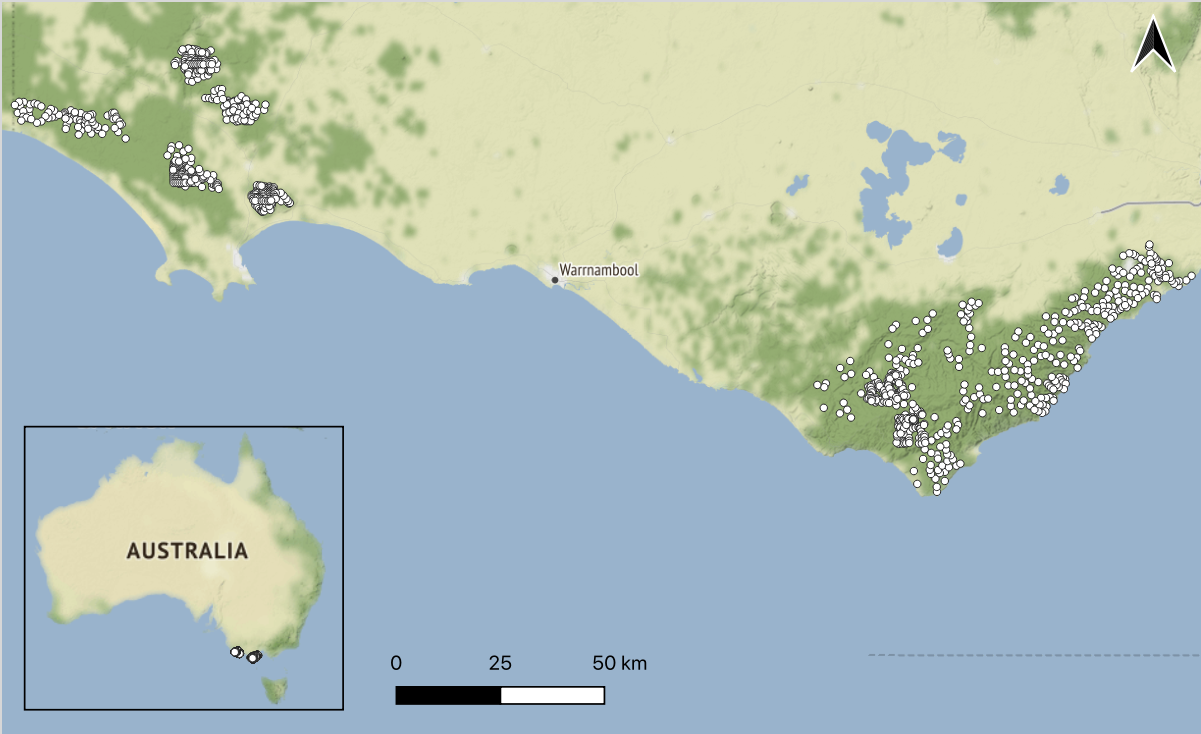
\includegraphics[width=1\linewidth]{figure/map_cams} 

}

\caption{Locations of study sites in south-west Victoria, Australia. The grids of camera-traps are denoted by white dots. The Glenelg region is to the west and Otway region to the east. Native vegetation is indicated by dark green, with hill shading. \textit{Map tiles by Stamen Design, under CC BY 3.0, map data by OpenStreetMap, under CC BY SA.}}\label{fig:occ-map}
\end{figure}
\newpage

\hypertarget{results-1}{%
\section{Results}\label{results-1}}

\hypertarget{red-fox-1}{%
\subsection{Red fox}\label{red-fox-1}}

\hypertarget{occupancy-detection-models-1}{%
\subsubsection{Occupancy-detection models}\label{occupancy-detection-models-1}}

Foxes were detected on 1,453 of the 3,667 camera-traps surveys (39.6\%; Table \ref{tab:occ-naive}). Fox detectability in unbaited landscapes was high, particularly in the Glenelg region (Fig. \ref{fig:occ-det}a) where 95\% detection probability was reached after a 30 day survey duration (relative to 64 days in the Otway Ranges; Fig. \ref{fig:occ-cumdet}). Fox control reduced fox detectability across both regions. Nonetheless, foxes in baited landscapes still had a high detection probability for the average survey duration (47 days): 76\% in the Glenelg region and 81\% in the Otway Ranges (Fig. \ref{fig:occ-cumdet}).

The occupancy-detection model estimated fox occupancy to be lower at sites in baited landscapes than unbaited landscapes; this effect was more than twice as strong in the Glenelg region than the Otway Ranges (Fig. \ref{fig:occ-det}b). For example, in heathy woodlands of the Glenelg region, fox occupancy probability was approximately three times lower in baited landscapes (0.19; 95\% CI 0.13 - 0.26) relative to unbaited landscapes (0.56; 95\% CI: 0.47 - 0.66). Whereas in the heathy woodlands of the Otway Ranges, fox occupancy was already low without fox control (0.33; 95\% CI: 0.25 - 0.43) and was approximately 1.4 times lower following fox control (0.24; 95\% CI 0.17 - 0.33). Foxes were ubiquitous across the study regions, but the probability of occupancy was nearly twice as high in dry forests, herb-rich woodlands and lowland forests than heathlands, heathy woodlands and wet forests (Fig. \ref{fig:occ-det}c).

\hypertarget{generalised-additive-models-1}{%
\subsubsection{Generalised additive models}\label{generalised-additive-models-1}}

The GAM showed that fox-bait density in the Glenelg region was the strongest driver of fox occurrence. Fox occurrence in the Glenelg region declined from a probability of 0.68 (95\% CI: 0.58 - 0.76) where fox-bait density was zero, to 0.04 (95\% CI: 0.02 - 0.11) where fox-bait density was highest (1.14 baits km\textsuperscript{-2}; Fig. \ref{fig:gams-occ-fox}a). The effect of fox-bait density on foxes in the Glenelg region was nonlinear: there was little difference in fox occurrence across the range of 0.4 to 0.8 baits km\textsuperscript{-2}, but a greater suppression was achieved at higher bait densities (Fig. \ref{fig:gams-occ-fox}a). Fox occurrence also declined with fox-bait density in the Otway Ranges, but this effect was linear, weaker and had higher uncertainty (Fig. \ref{fig:gams-occ-fox}a). In the Otway Ranges, fox occurrence declined from a probability of 0.4 (95\% CI: 0.32 - 0.48) where fox-bait density was zero, to 0.14 (95\% CI: 0.05 - 0.35) where fox-bait density was highest (1.1 baits km\textsuperscript{-2}; Fig. \ref{fig:gams-occ-fox}a).

There was no average TSF response on fox occurrence, however, fox occurrence declined linearly with TSF in dry forests and increased linearly with TSF in heathland, although there was considerable uncertainty in these estimates (Fig. \ref{fig:gams-occ-fox}g:h).

Fox occurrence declined linearly with increasing terrain ruggedness, and with distance to non-native vegetation for distances up to approximately 1.5 - 2 km (Fig. \ref{fig:gams-occ-fox}d;f). Elevation had a nonlinear and uncertain effect on fox occurrence, which was estimated to peak around 450 m above sea level (Fig. \ref{fig:gams-occ-fox}c). The effect of topographic wetness on fox occurrence was removed from the model (Fig. \ref{fig:gams-occ-fox}e). The fox GAM that considered rainfall deviations in the previous 6 months was ranked highest relative to models with 18- (by only 1.4 AIC units), 12-, and 24-month periods (by at least 6.4 AIC units; Table. \ref{tab:occ-rain-aic}); however, this effect was weak with relatively high uncertainty (Fig. \ref{fig:gams-occ-fox}c).

The top-ranked fox GAM had an adjusted R-square value of 0.27 and explained 26\% of the null deviance. Relative to the null model (with only a site random intercept), the explanatory variables improved predictive performance considerably (242 AIC units lower), but slightly worsened the model fit (Table. \ref{tab:occ-model-sumstats}).

\hypertarget{feral-cat-1}{%
\subsection{Feral cat}\label{feral-cat-1}}

\hypertarget{occupancy-detection-models-2}{%
\subsubsection{Occupancy-detection models}\label{occupancy-detection-models-2}}

Cats were detected on 1,010 camera-trap deployments (27.6\%; Table \ref{tab:occ-naive}). Cats were relatively poorly detected in the Glenelg region, where they had a 59\% detection probability given presence for the average survey duration, compared to 83\% in the Otway Ranges; Fig. \ref{fig:occ-cumdet}). There was no detectability difference between fox control treatment landscapes in the Glenelg region, however, cat detectability was slightly higher with fox control in the Otway Ranges (Fig. \ref{fig:occ-det}a).

The occupancy-detection models estimated that cat occupancy in the Glenelg region was higher in landscapes with fox control (e.g., 0.25 in heathy woodlands; 95\% CI: 0.16 - 0.35 in heathy woodlands) relative to those without fox control (0.12 in heathy woodlands; 95\% CI: 0.07 - 0.19); but there was no association with baiting in the Otway Ranges (Fig. \ref{fig:occ-det}b). Cat occupancy was most strongly driven by vegetation type: highest in the wet forest, followed by heathland, swampy scrub, herb-rich woodland and dry forest, but very low in lowland forest and heathy woodland (Fig. \ref{fig:occ-det}c).

\hypertarget{generalised-additive-models-2}{%
\subsubsection{Generalised additive models}\label{generalised-additive-models-2}}

The cat GAM showed no effect of fox-bait density, elevation or topographic wetness on cat occurrence (Fig. \ref{fig:gams-occ-cat}a;c;e). Cats responded to TSF differently across each vegetation type, with the average TSF response removed from the model (Fig. \ref{fig:gams-occ-cat}g:h). Cat occurrence probability increased with terrain ruggedness, and declined with distance from the nearest area of non-native vegetation, although uncertainty was high (Fig. \ref{fig:gams-occ-cat}d;f). The different rainfall deviation windows were were indistinguishable based on AIC scores; but in all cases except 6 months, the rainfall variable was removed from the model. The model that considered rainfall deviations in the previous six months was marginally top-ranked (by 0.7 AIC units) and estimated that cat occurrence slightly increased as rainfall increased (relative to the long-term average; Fig. \ref{fig:gams-occ-cat}c).

The top-ranked cat GAM had an adjusted R-square value of 0.24 and explained 24\% of the null deviance. Relative to the null model, the explanatory variables improved predictive performance considerably (168 AIC units lower), but only slightly improved the model fit (less than 1\% increase in null deviance explained and 0.02 for the R-squared value; Table. \ref{tab:occ-model-sumstats}).

\hypertarget{southern-brown-bandicoot-1}{%
\subsection{Southern brown bandicoot}\label{southern-brown-bandicoot-1}}

\hypertarget{occupancy-detection-models-3}{%
\subsubsection{Occupancy-detection models}\label{occupancy-detection-models-3}}

We detected SBBs on 394 of the 3,667 camera-traps (10.7\%; Table \ref{tab:occ-naive}). SBBs were highly detectable, with a greater than 95\% detection probability reached after 31 and 43 days in the Glenelg and Otway Ranges, respectively (Fig. \ref{fig:occ-cumdet}). Baiting was associated with a decrease in SBB detectability in Glenelg but an increase in detectability in the Otways (Fig. \ref{fig:occ-det}a).

There was no discernible effect of fox control on SBB occupancy in either region (Fig. \ref{fig:occ-det}b). SBB's were most likely to occupy heathy woodlands (Fig. \ref{fig:occ-det}c) and they were largely absent from wet forests (Table \ref{tab:occ-naive}). The few SBB detections in wet forest occurred at sites adjacent to other vegetation types (SBBs are largely replaced by long-nosed bandicoots \emph{Perameles nasuta} in wet forest; M. Rees, unpublished data).

\hypertarget{generalised-additive-models-3}{%
\subsubsection{Generalised additive models}\label{generalised-additive-models-3}}

SBB occurrence probability was very low. There was some indication SBB occurrence slightly increased with fox-bait density in the Glenelg region, peaking at around 150 m above sea level and 2 km from the nearest forest edge and declined with increasing terrain ruggedness and TSF; however, these explanatory variables had high uncertainty relative to the strength of the effects (Fig. \ref{fig:gams-occ-sbb}). There was no evidence that rainfall affected SBB occurrence -- the top-ranked models in terms of AIC scores (Table. \ref{tab:occ-rain-aic}) had the effects of rainfall completely removed.

The top-ranked SBB GAMs had an adjusted R-square value of 0.31 and explained 41\% of the null deviance. Relative to the null model, the explanatory variables improved predictive performance considerably (211 AIC units lower) and slightly improved the model fit by 4\% of null deviance explained and 0.05 for the R-squared value (Table. \ref{tab:occ-model-sumstats}).

\hypertarget{long-nosed-potoroo-1}{%
\subsection{Long-nosed potoroo}\label{long-nosed-potoroo-1}}

\hypertarget{occupancy-detection-models-4}{%
\subsubsection{Occupancy-detection models}\label{occupancy-detection-models-4}}

We detected LNPs on 331 camera-trap deployments (9\%; Table \ref{tab:occ-naive}). LNPs were the most detectable of our study species, reaching a 95\% detection probability with a 33 and 18 day survey duration in the unbaited landscapes of the Glenelg and Otway regions, respectively (Fig. \ref{fig:occ-cumdet}). In the Glenelg region, LNP detectability was twice as high in landscapes with fox control relative to those without (Fig. \ref{fig:occ-det}a). Occupancy of LNPs was highest in heathlands (Fig. \ref{fig:occ-det}c).

\hypertarget{generalised-additive-models-4}{%
\subsubsection{Generalised additive models}\label{generalised-additive-models-4}}

The GAM showed that LNP occupancy improved from a 0.05 probability (95\% CI: 0.02 - 0.11) to 0.33 (95\% CI: 0.16 - 0.55) across the fox-bait density gradient in the Glenelg region (Fig. \ref{fig:gams-occ-lnp}a). In contrast, LNP occupancy showed no relationship with poison-bait density in the Otway region (Fig. \ref{fig:gams-occ-lnp}a). LNP occurrence probability increased linearly with elevation (Fig. \ref{fig:gams-occ-lnp}c) and peaked in the mid-range of topographic wetness (Fig. \ref{fig:gams-occ-lnp}e). LNP occurrence was low initially after fire, but peaked around 20 years and remained steady in the years afterwards, although there was considerably uncertainty (Fig. \ref{fig:gams-occ-lnp}e). There were no discernible differences in LNP responses to TSF across the vegetation types (Fig. \ref{fig:gams-occ-lnp}f). The rainfall term was removed for the top-ranked model (at least 3.5 AIC units higher than models that included it).

The top-ranked model had an adjusted R-square value of 0.47 and explained 53\% of the null deviance. Relative to the null model, the explanatory variables improved predictive performance (94 AIC units lower) and slightly improved the model fit by 3\% of null deviance explained and 0.02 for the R-squared value (Table. \ref{tab:occ-model-sumstats}).

\newpage
\begin{figure}

{\centering 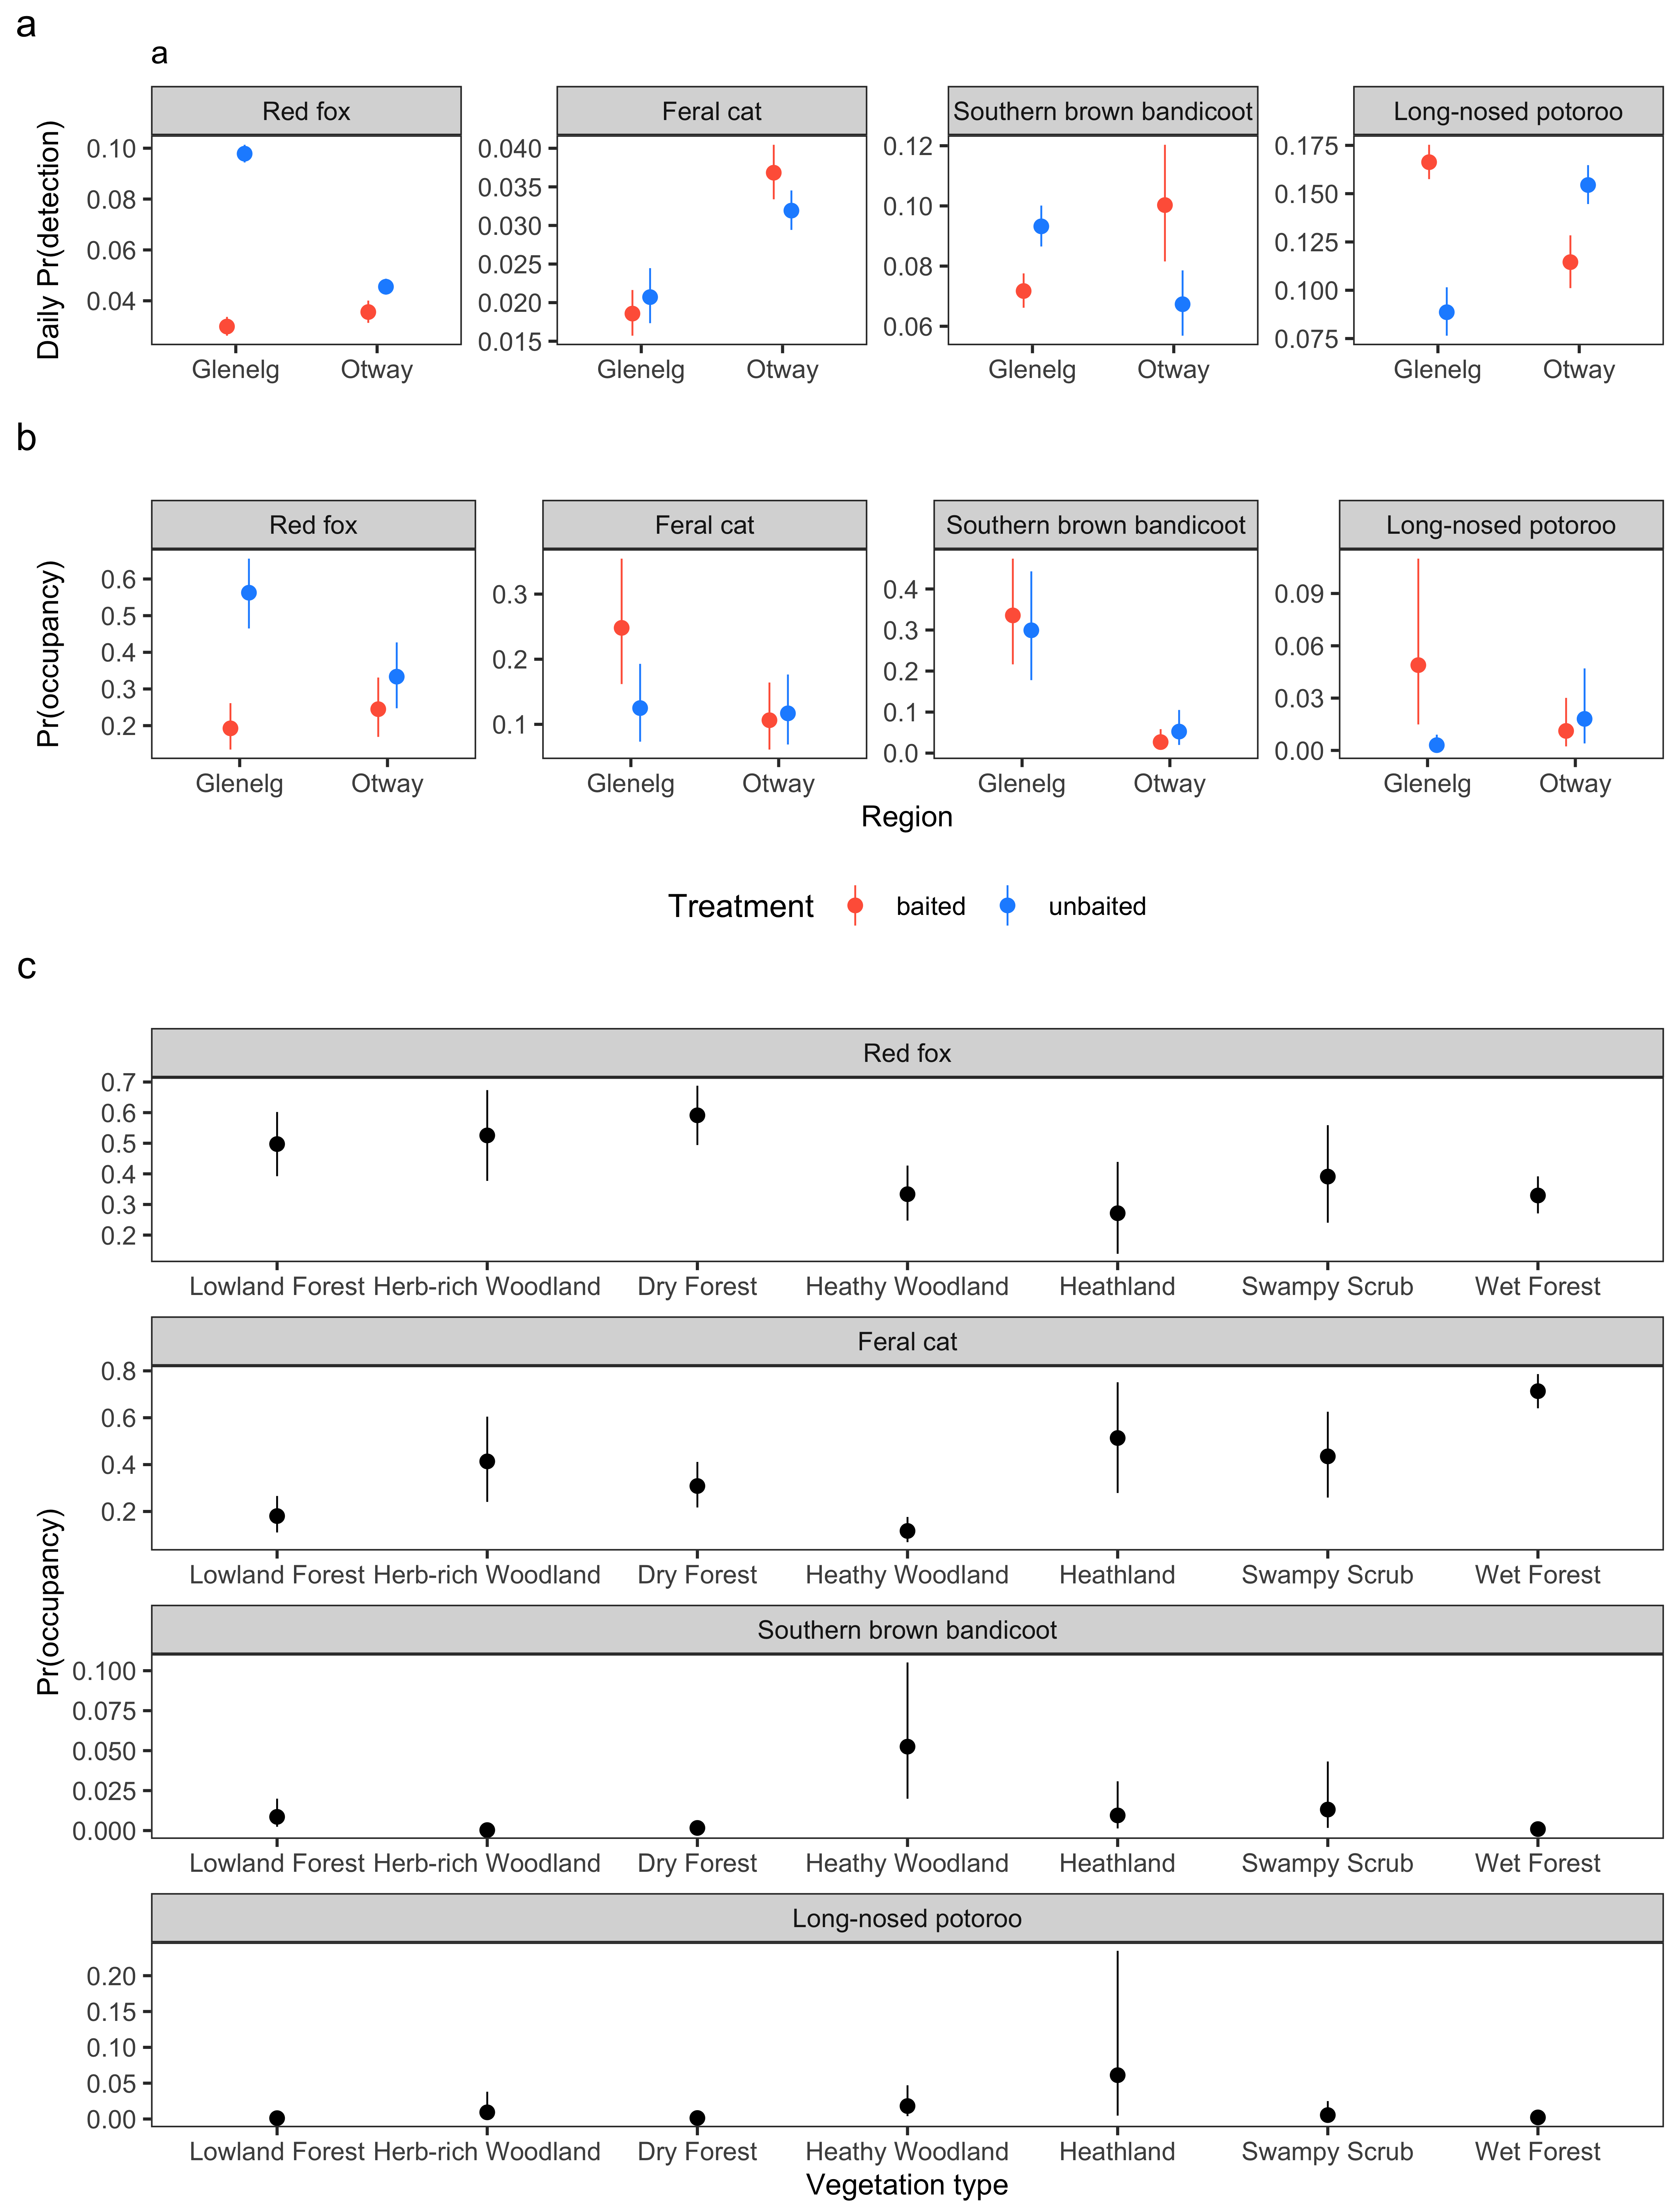
\includegraphics[width=1\linewidth]{figure/occ_det_ubms} 

}

\caption{Outputs from Bayesian occupancy-detection for each study species. Daily detection probabilities (a) and occupancy estimates (b) in landscapes with fox control (red) and without fox control (blue) in the Glenelg region and Otway Ranges, south-west Victoria, Australia (with Heathy Woodlands as a reference level). Fox control had occurred in The Glenelg region for 8 - 13 years and was monitored with a control-impact design. The Otway Ranges was monitored using a before-after-control-impact experimental design; surveyed approximately 1 year prior and 2 years following the commencement of fox-baiting. Occupancy was also modelled as a function of vegetation type (Ecological Vegetation Class groups; c). Error bars represent 95\% Bayesian credible intervals.}\label{fig:occ-det}
\end{figure}
\newpage
\begin{figure}

{\centering 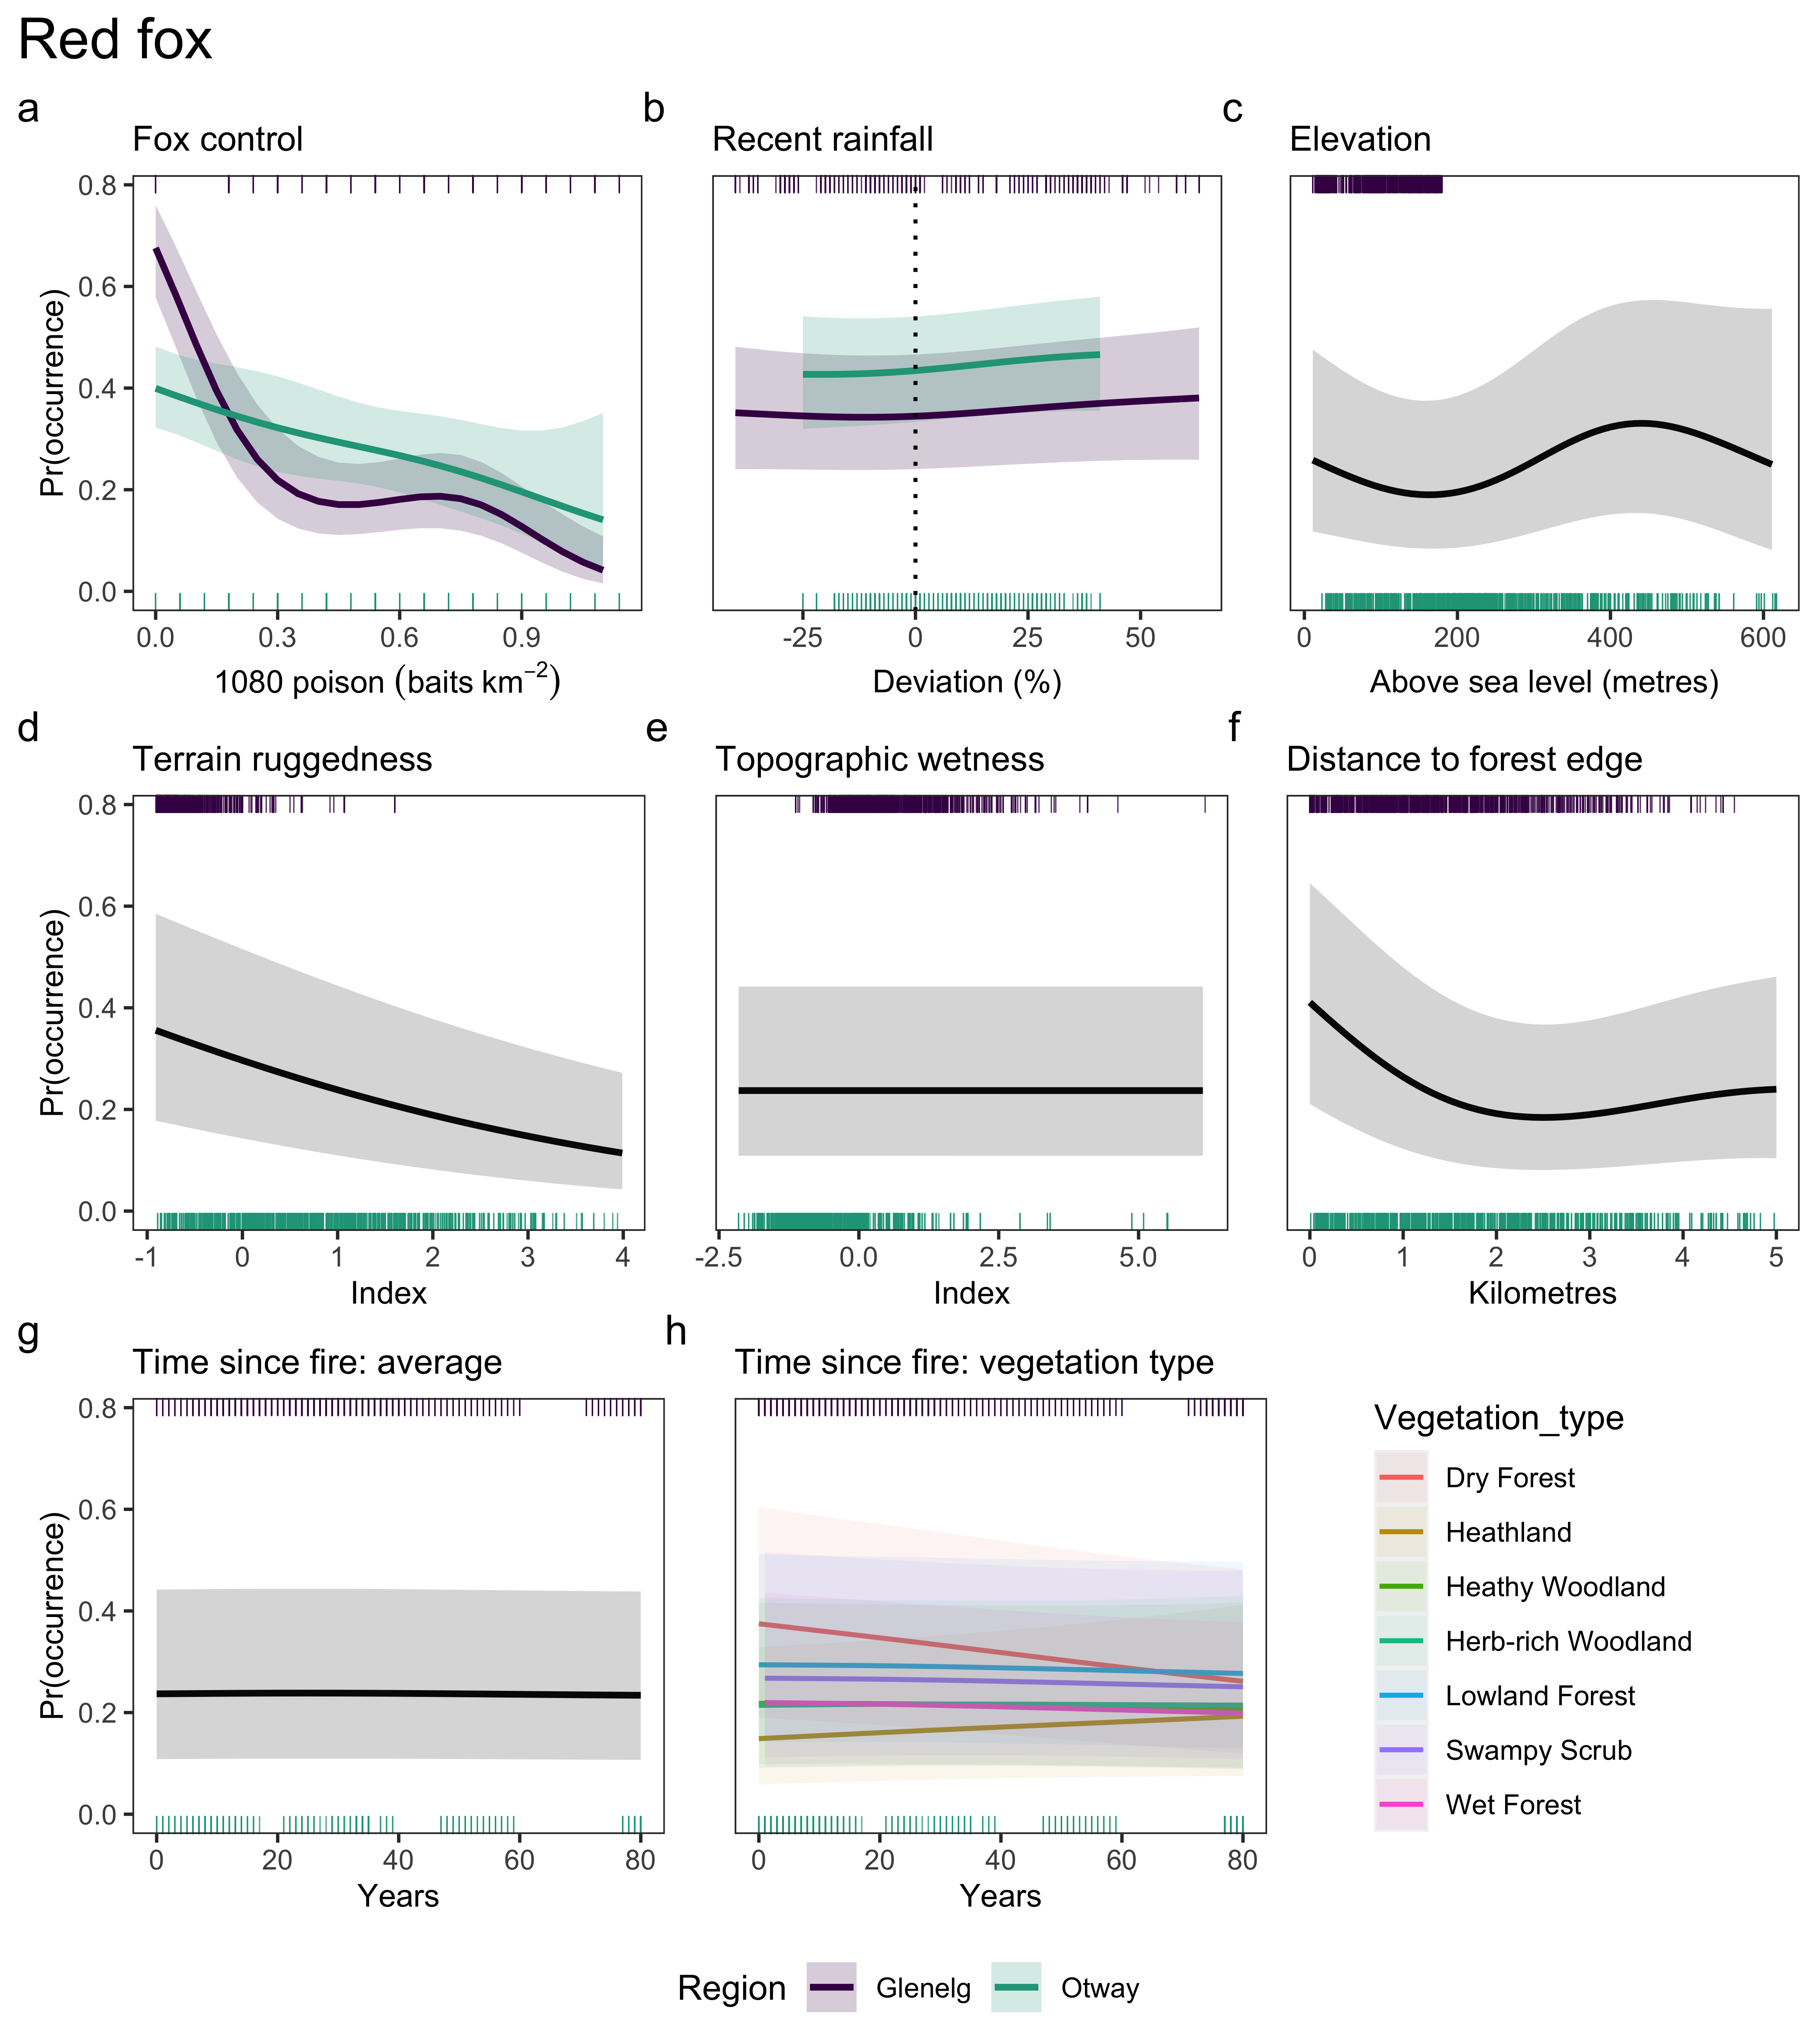
\includegraphics[width=1\linewidth]{figure/gams_fox} 

}

\caption{Generalised additive model estimates of the effect of each explanatory variable (columns) on red fox \textit{Vulpes vulpes} occurrence. Shaded bands indicate 95\% confidence intervals.}\label{fig:gams-occ-fox}
\end{figure}
\newpage
\begin{figure}

{\centering 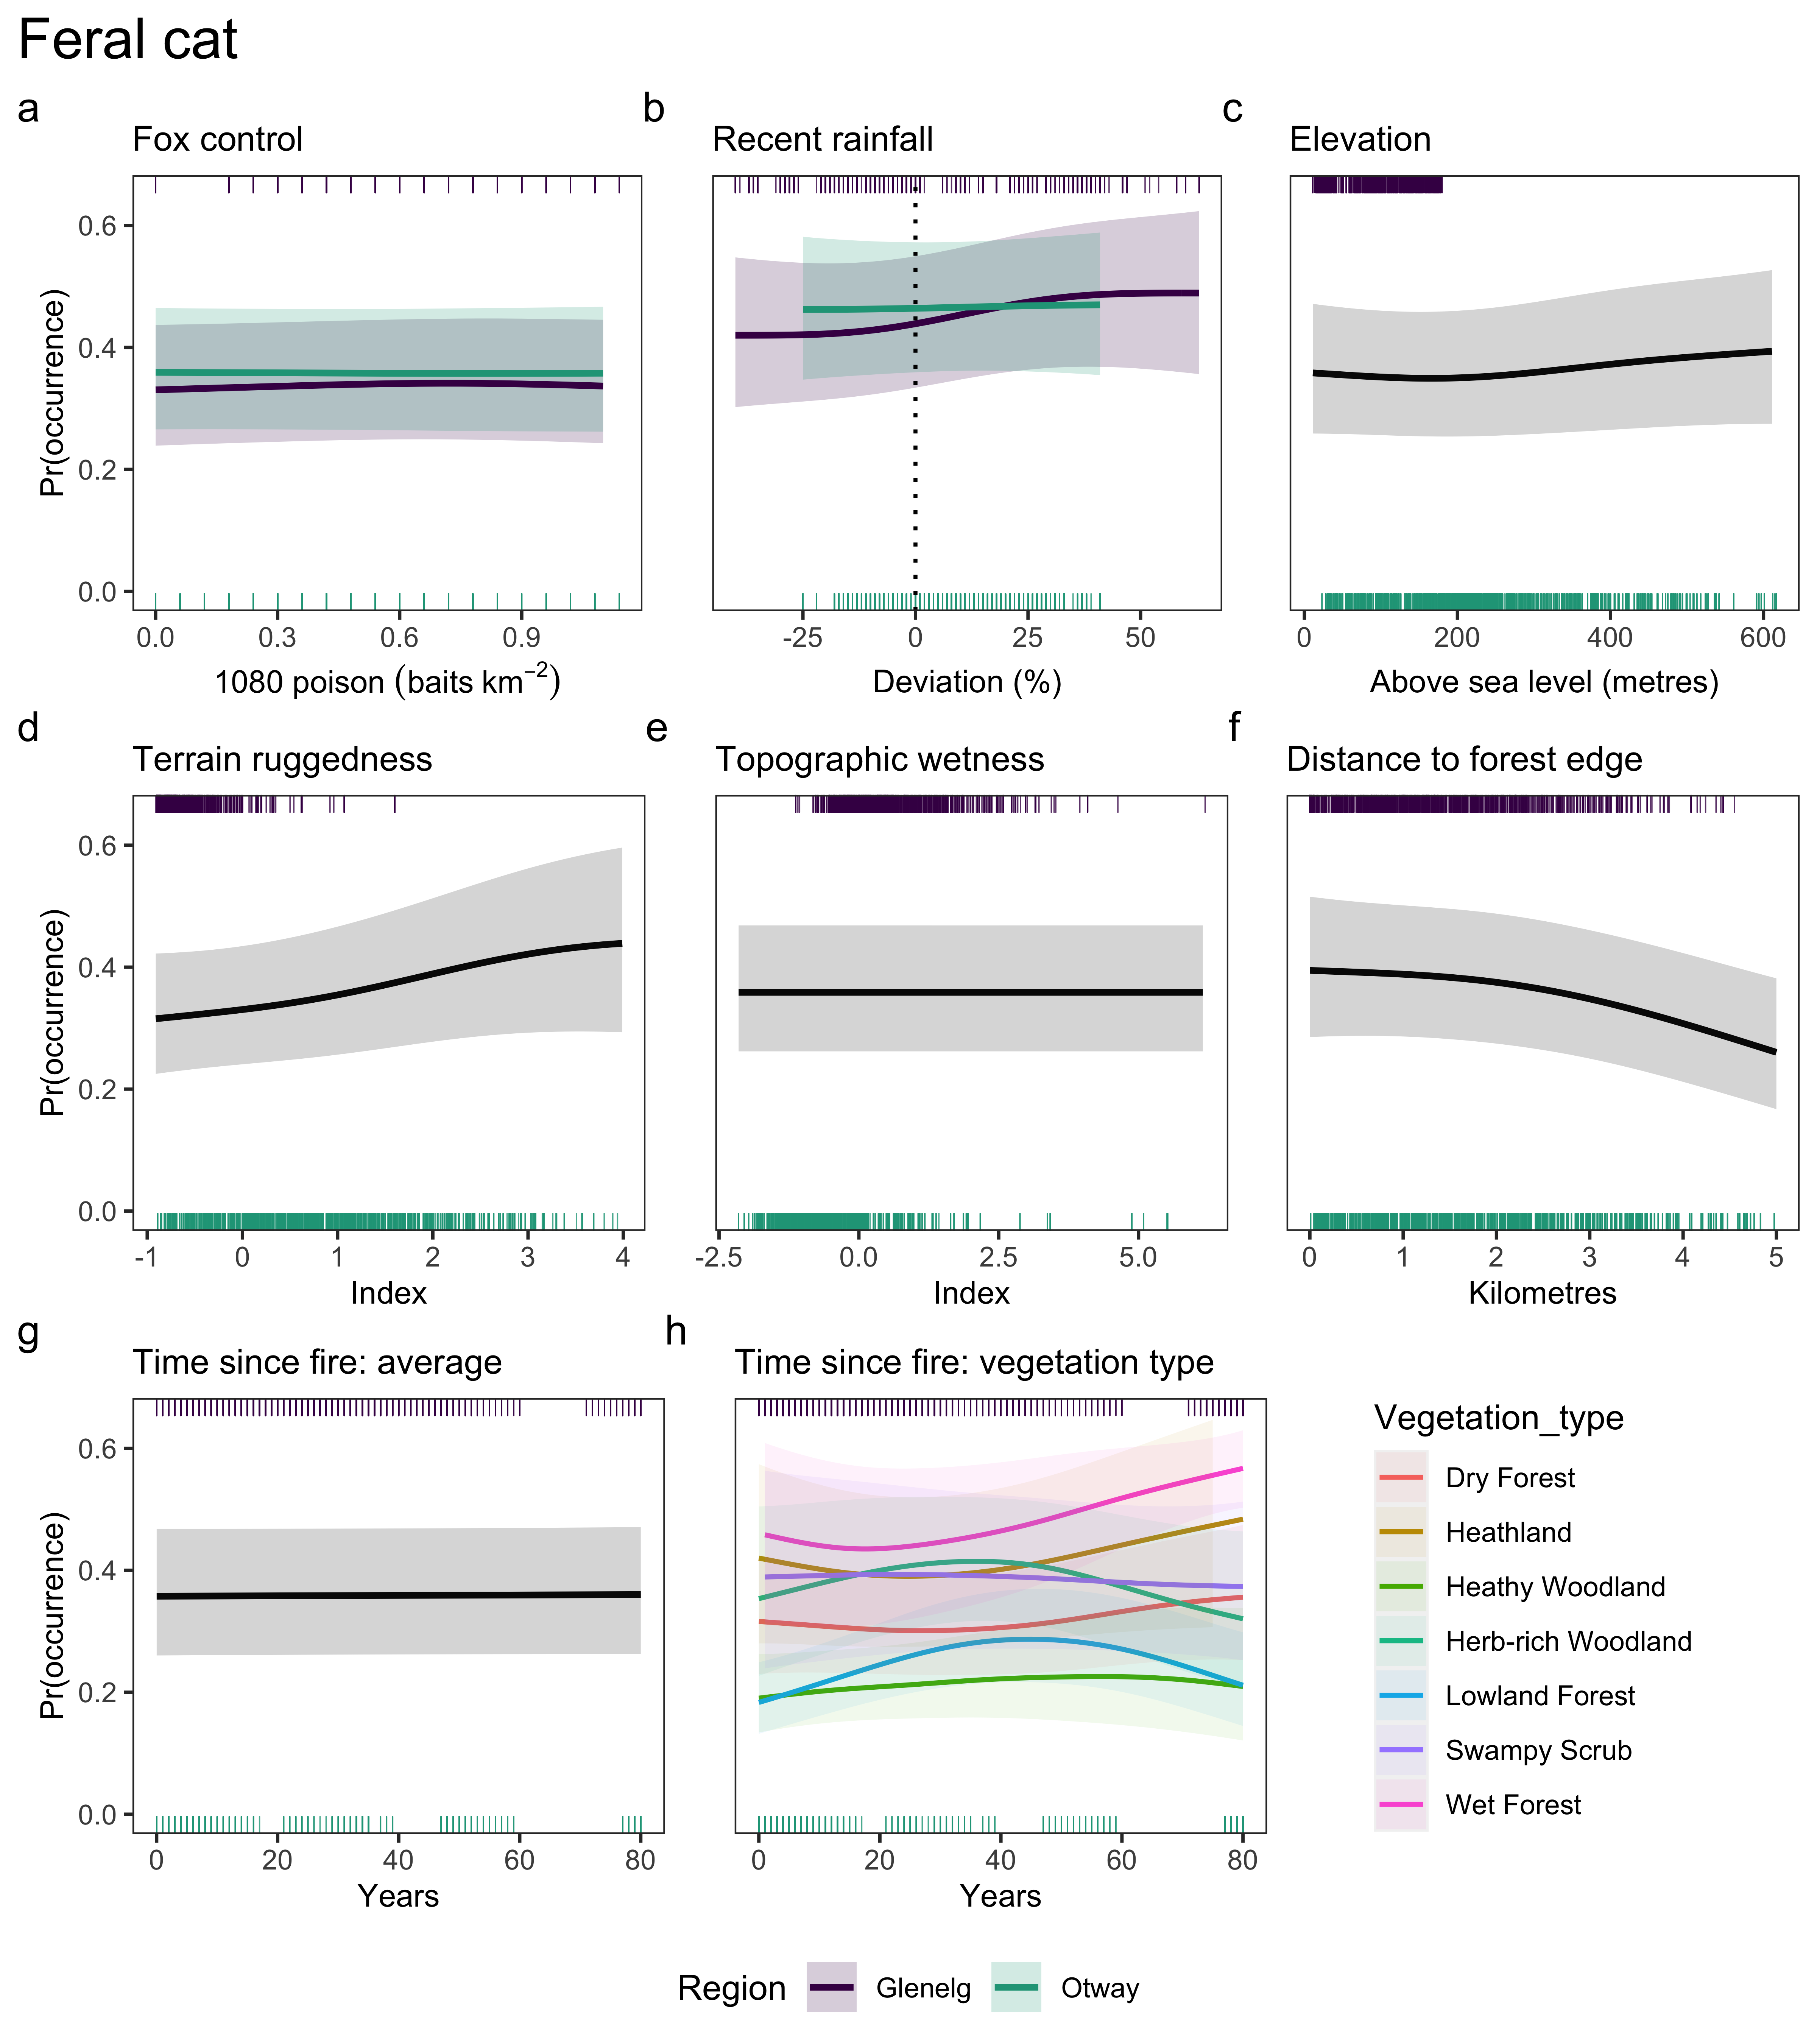
\includegraphics[width=1\linewidth]{figure/gams_cat} 

}

\caption{Generalised additive model estimates of the effect of each explanatory variable (columns) on feral cat \textit{Felis catus} occurrence. Shaded bands indicate 95\% confidence intervals.}\label{fig:gams-occ-cat}
\end{figure}
\newpage
\begin{figure}

{\centering 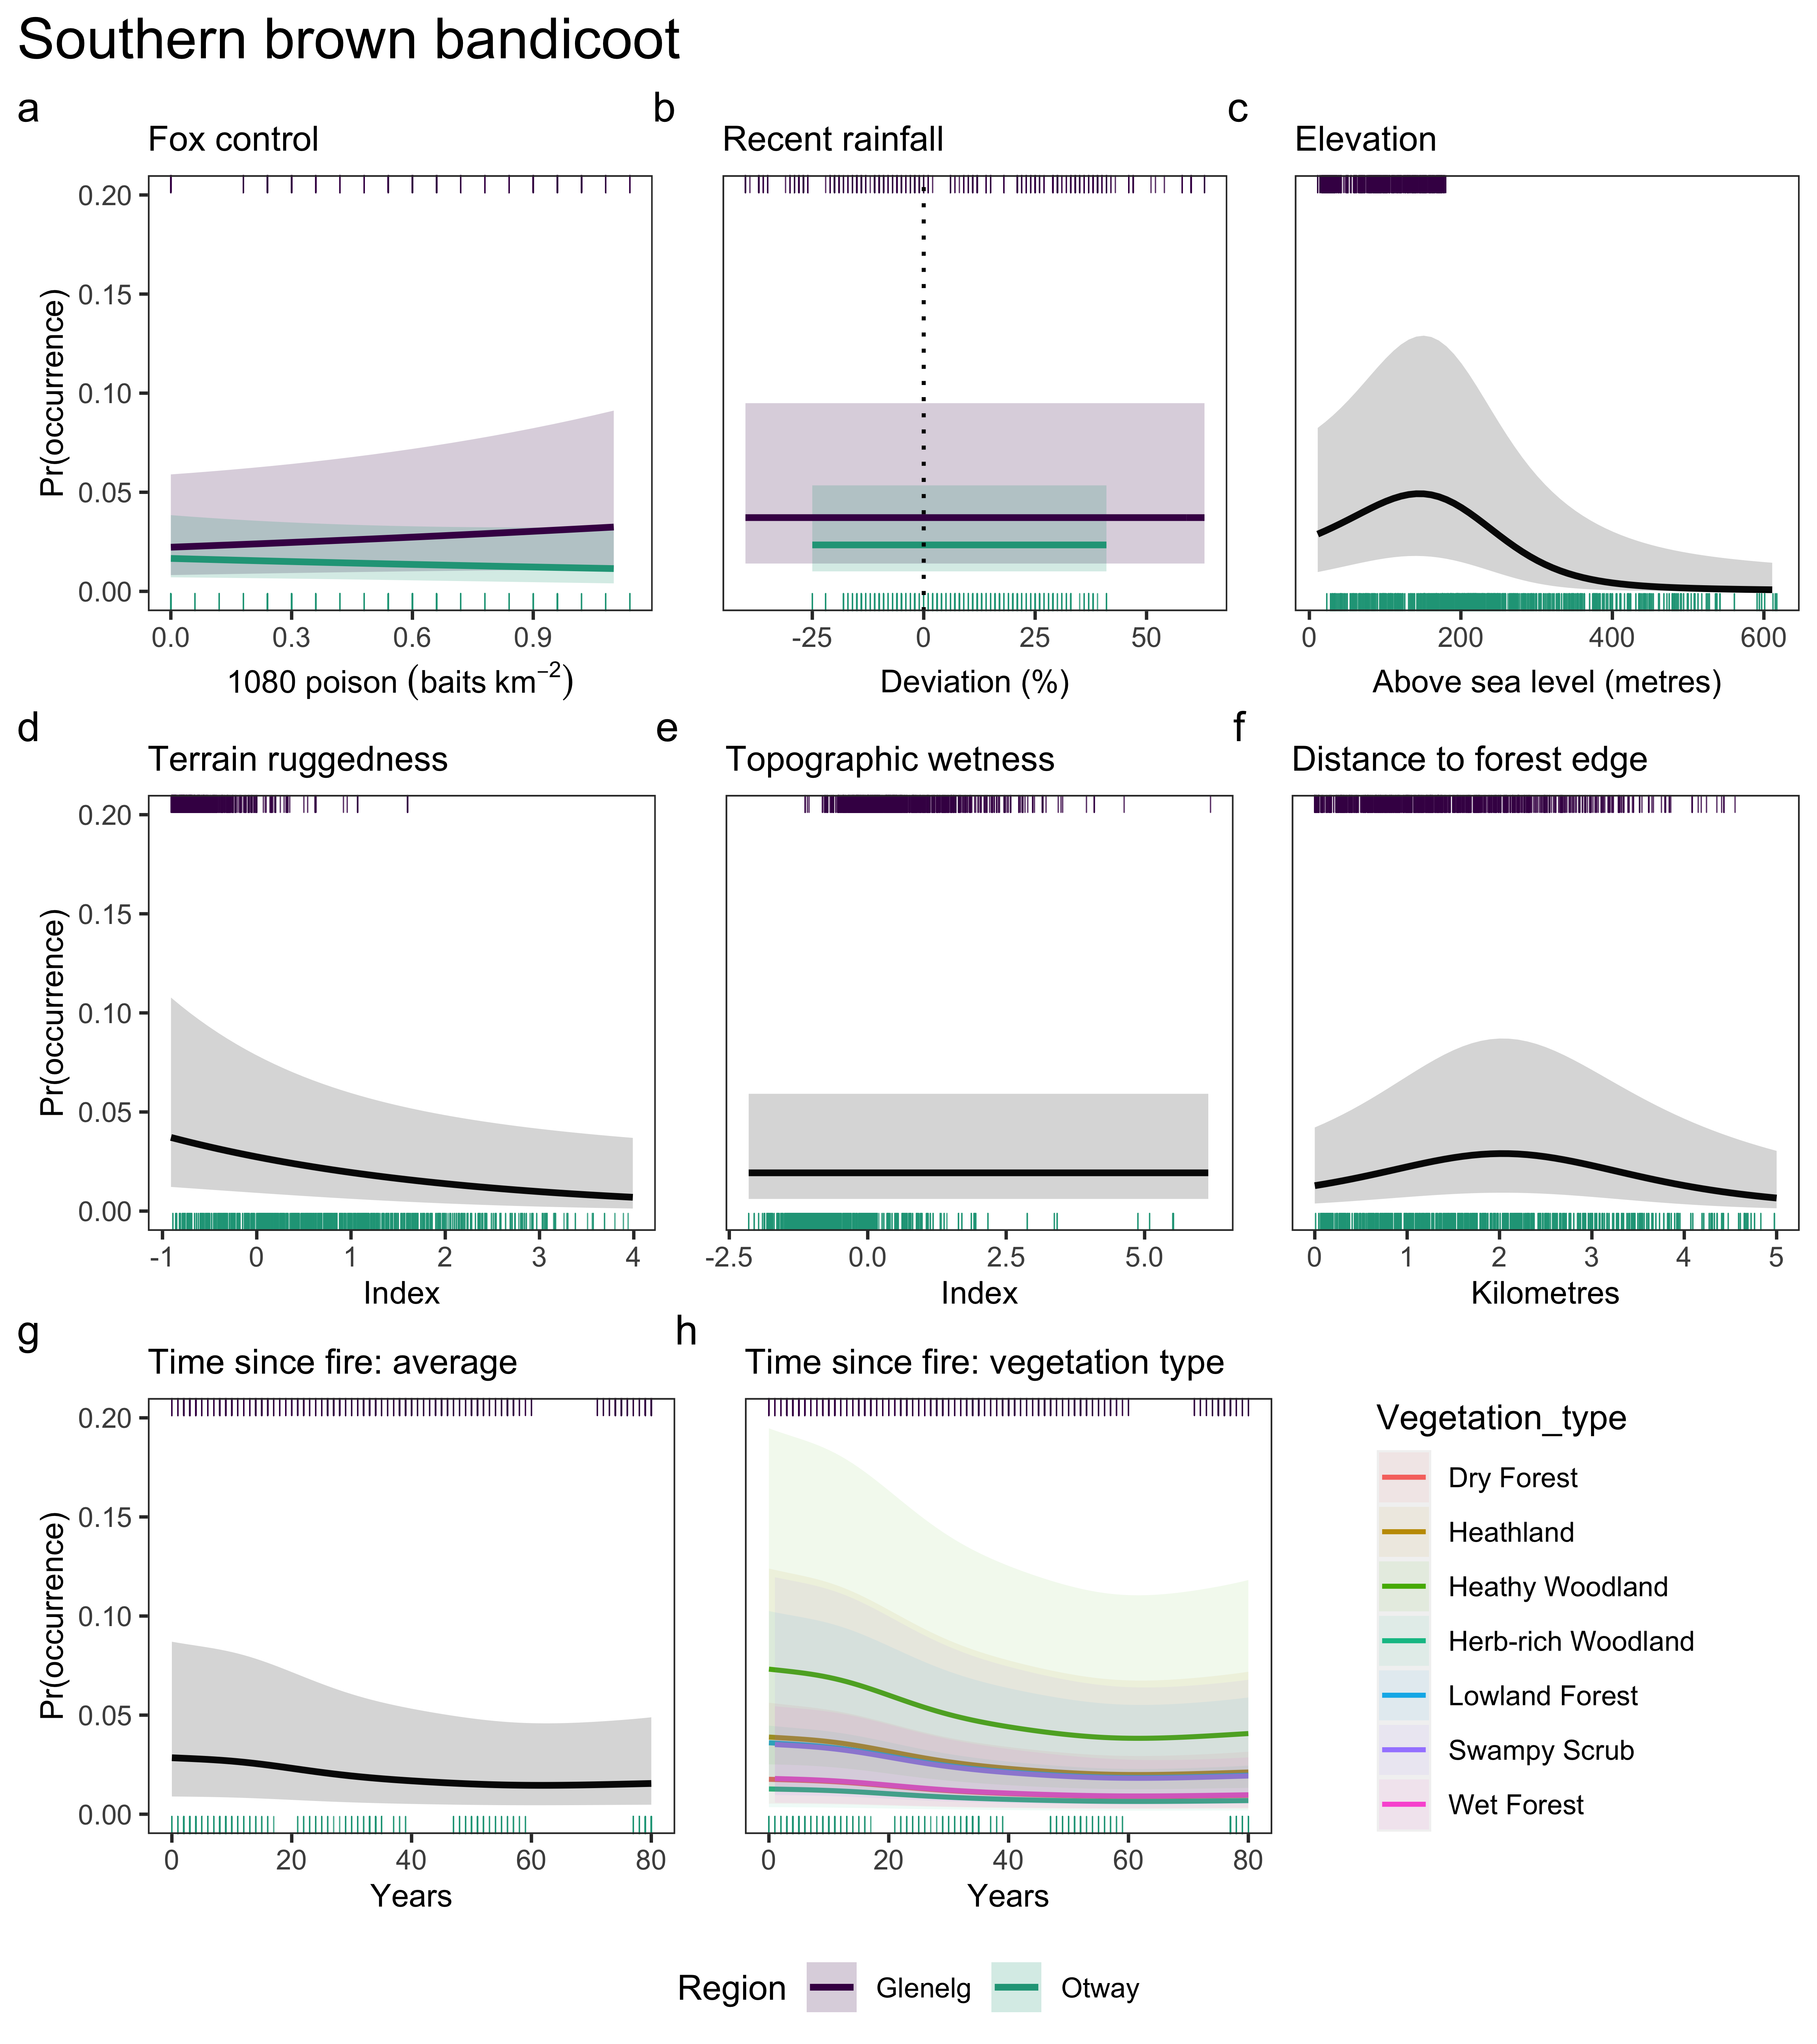
\includegraphics[width=1\linewidth]{figure/gams_sbb} 

}

\caption{Generalised additive model estimates of the effect of each explanatory variable (columns) on southern brown bandicoot \textit{Isoodon obesulus} occurrence. Shaded bands indicate 95\% confidence intervals.}\label{fig:gams-occ-sbb}
\end{figure}
\newpage
\begin{figure}

{\centering 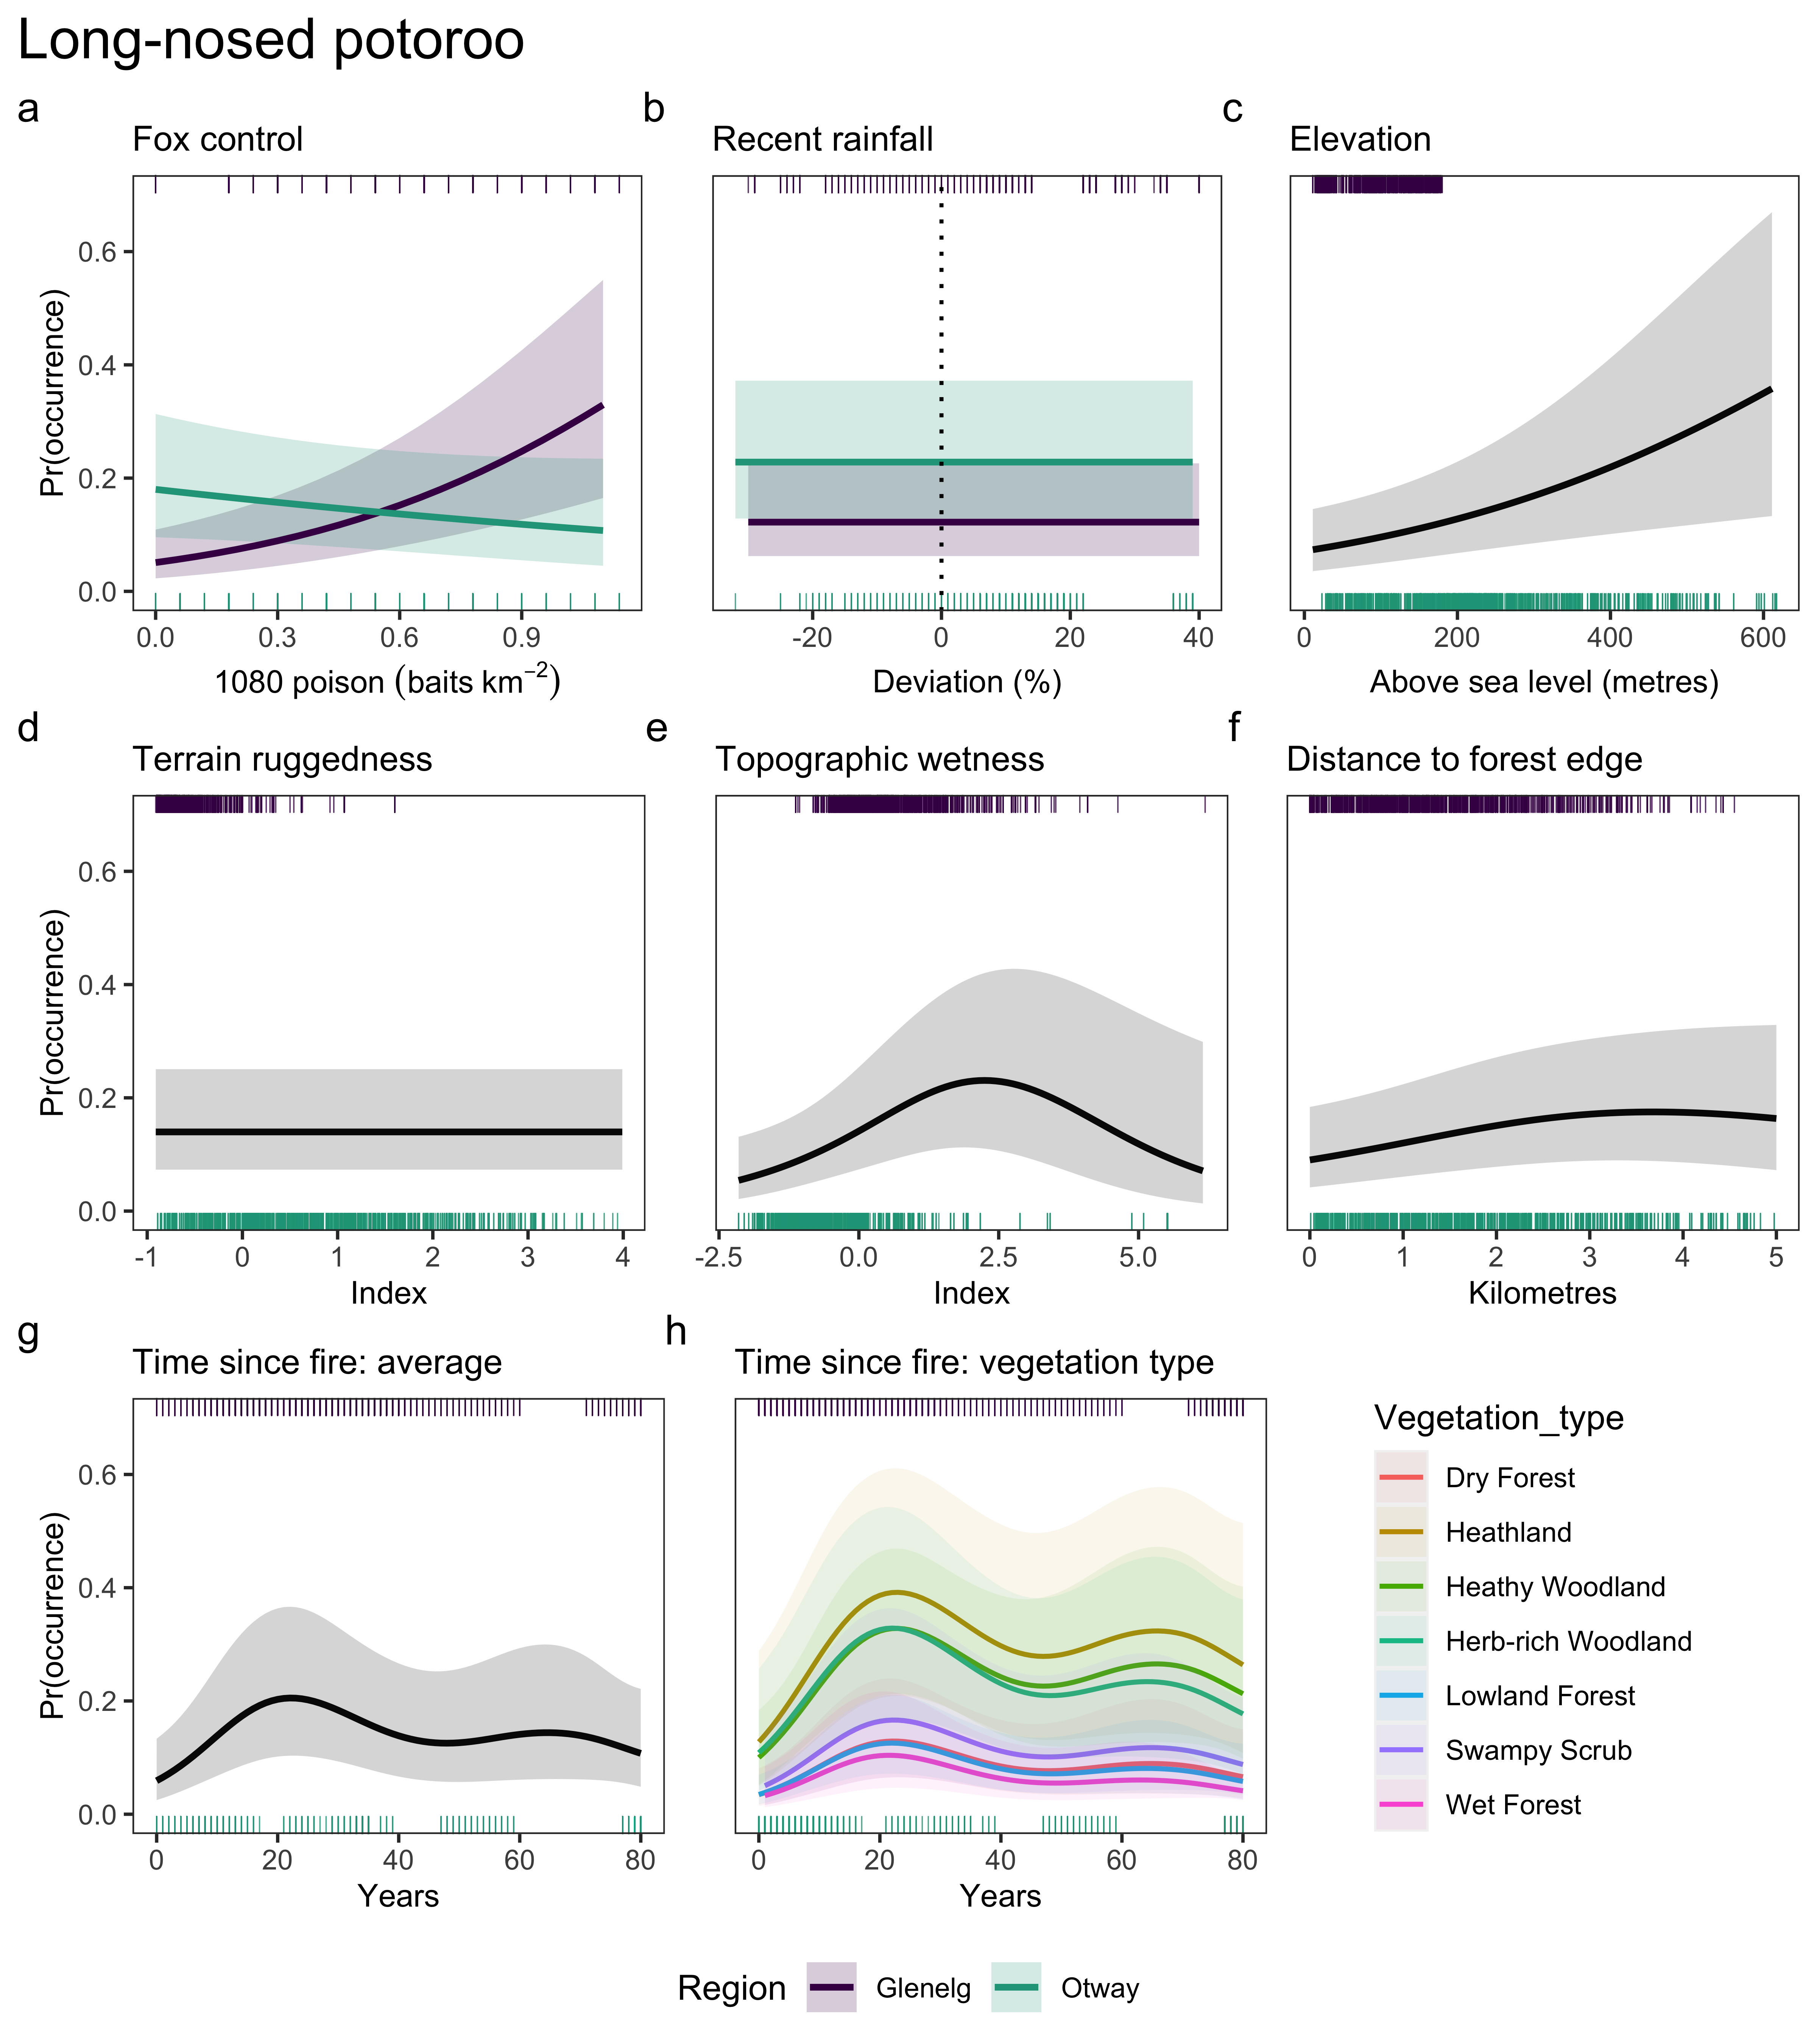
\includegraphics[width=1\linewidth]{figure/gams_lnp} 

}

\caption{Generalised additive model estimates of the effect of each explanatory variable (columns) on long-nosed potoroo \textit{Potorous tridactylus} occurrence. Shaded bands indicate 95\% confidence intervals.}\label{fig:gams-occ-lnp}
\end{figure}
\newpage

\hypertarget{discussion-1}{%
\section{Discussion}\label{discussion-1}}

Here we found that consistent and long-term lethal control can reduce a widespread invasive apex predator (fox) to a near-zero occurrence probability---and importantly---increase the occurrence probability of a threatened prey species (LNP) by more than 6-fold (Fig. \ref{fig:gams-occ-fox}a; Fig. \ref{fig:gams-occ-lnp}a). However, prey responses to predator suppression are not universal (Sinclair \emph{et al.} 1998; Duncan \emph{et al.} 2020). Despite increasing site occupancy in the early stages of the Glenelg Ark fox baiting program (Robley \emph{et al.} 2014), we found little evidence that SBB occupancy increased with fox control in either region (Fig. \ref{fig:occ-det}b; Fig. \ref{fig:gams-occ-lnp}a). This may have been because feral cat occupancy was twice as high in the landscapes with fox control relative to those without in the Glenelg region (Fig. \ref{fig:occ-det}b), potentially signalling mesopredator release. In the Otway region (where fox control recently commenced and baiting was less frequent), foxes were suppressed to a lesser extent (as expected) and neither threatened prey species showed signs of improvement (Fig. \ref{fig:occ-det}b; Fig. \ref{fig:gams-occ-fox}a; Fig. \ref{fig:gams-occ-sbb}a; Fig. \ref{fig:gams-occ-lnp}a). Our study demonstrates that lethal invasive predator control can be a highly effective conservation strategy, but only for some species and when sustained continuously over the long-term.

The Glenelg Ark program has continuously controlled foxes across approximately 100,000 ha of public land since 2005 (Robley \emph{et al.} 2014) and is one of the few fox control programs in Australia to demonstrate a sustained reduction in fox occupancy (see also Stobo-Wilson \emph{et al.} 2020a). A reduction in fox occupancy is a strong sign of management effectiveness because it means prey are less exposed to the threat of predation. Our study provides empirical evidence that the effectiveness of fox control from poison-baiting programs depends on the density of poison-baits deployed (Fig. \ref{fig:gams-occ-fox}a). This has only previously been inferred by comparing fox baiting programs across different regions (where fox ecology, environmental conditions and study designs differ). The densities of poison-baits in our study regions (maximum 1.14 baits km\textsuperscript{-2}) were far below the recommended 5 - 10 baits km\textsuperscript{-2} (mostly derived from studies in arid and semi-arid regions, Saunders \& McLeod 2007), but nonetheless effective at fox suppression in the Glenelg region (Fig. \ref{fig:occ-det}b). Increasing bait density up to 0.3 baits km\textsuperscript{-2} was particularly effective at controlling foxes in the Glenelg region, reducing fox occurrence by up to four-fold compared to unbaited regions; afterwards, increasing poison-bait densities continued to suppress foxes, but with a weaker effect (Fig. \ref{fig:gams-occ-fox}a). Increased bait caching at high bait densities may explain why fox suppression tapered off, which is likely to result in a sublethal dose when eventually consumed and potential bait aversion (Saunders \& McLeod 2007). Nonetheless, benefits to threatened native prey is the best metric of fox control effectiveness. The probability of LNP occurrence increased linearly with poison-bait density in the Glenelg region (Fig. \ref{fig:gams-occ-lnp}a), confirming that high fox control effort leads to improved conservation outcomes.

We slightly underestimated the effect of bait density across both regions because the models assumed all bait-stations were constantly active, despite some bait-replacements being missed due to accessibility issues following wet weather events or because of more pressing management concerns (namely wildfire). We more strongly underestimated the effect of bait density in the Otway Ranges because we also did not account for a near six-month pause in bait replacement in 2018. We also expect fox-baits to be less effective in the Otway Ranges than the Glenelg region due to the higher rainfall which more quickly degrades the poison (Saunders, McLeod, \& Kay 2000; Gentle, Saunders, \& Dickman 2007b). Nonetheless, fox occupancy in the Otway Ranges was still negatively associated with fox-bait density (Fig. \ref{fig:gams-occ-fox}a), suggesting that intensified and sustained fox control is likely to be effective in that region. Future research will benefit from accounting for the role of environmental conditions and prey availability on baiting effectiveness (Saunders \& McLeod 2007; Carter \& Luck 2013), as well as interference with baits by non-target species (Fairbridge \emph{et al.} 2000; Glen \& Dickman 2003; Marlow \emph{et al.} 2015b).

Evidence that fox control caused mesopredator release of feral cats in terms of detectability and occupancy was mixed. Cat occupancy was higher in sites with fox control in the Glenelg region and cat detectability increased with fox control in the Otway Ranges (Fig. \ref{fig:occ-det}a:b). However, cat occurrence did not change across gradients of poison-bait density in either region (GAM; Fig. \ref{fig:gams-occ-cat}a). Cat detectability in the Glenelg region was very low (Fig. \ref{fig:occ-det}a), and so the model assumption of perfect detection in the cat GAM was likely problematic. This result could also signal that cats respond to fox suppression at the landscape level rather than at finer spatial scales. In addition, potential changes in population density and behaviour following mesopredator release (Brashares \emph{et al.} 2010), such as cats reducing their ranging behaviour following fox control (as found by Molsher \emph{et al.} 2017), could skew inference around occupancy estimates (Efford \& Dawson 2012; McCarthy \emph{et al.} 2013; Neilson \emph{et al.} 2018; Stewart \emph{et al.} 2018; Broadley \emph{et al.} 2019). Cats had weak associations with most explanatory variables, the poorest detection rates and worst model fits of our study species, further highlighting the challenges of monitoring this elusive, generalist predator (Fisher \emph{et al.} 2015; Stokeld \emph{et al.} 2015; Algar \emph{et al.} 2020).

In the Glenelg region, LNP---but not SBB---occupancy improved with fox control (Fig. \ref{fig:occ-det}b). Using increases in prey occupancy to measure the effectiveness of predator control rests on the assumption that there is suitable habitat for prey to expand into. While SBBs had a narrower distribution relative to LNPs across our study regions (largely absent from wet forests), there were 34 heathy woodland sites in the Glenelg region where they were never observed (from 196 camera-trap deployments), suggesting there may have been suitable habitat for them to colonise. However, EVCs such as ``heathy woodland'' are a coarse, model-generated categories; there may have been an environmental variable which precluded SBB presence at these 34 sites, such as local habitat structure (Swan \emph{et al.} 2015), although Smith (2013) found no association between habitat structure and SBB occupancy in the 240 Glenelg Ark monitoring sites. Alternatively, the different prey responses in our study could reflect the relative vulnerability of these species to fox and cat predation: LNPs (and other small macropods) appear more strongly limited by fox predation, whereas SBBs tend to be more closely associated with cat populations (Arthur, Catling, \& Reid 2012; Hunter \emph{et al.} 2018) and so may have experienced negative consequences from higher cat occupancy in Glenelg landscapes with fox control. This would also help explain why SBB occupancy was highest in heathy woodlands, where cat occupancy was lowest (Fig. \ref{fig:occ-det}c). Formally testing whether invasive predator occupancy impacts the probability of prey occupancy using multispecies models (Rota \emph{et al.} 2016) is a priority for future research.

In the Otway Ranges, fox control did not improve SBB or LNP occupancy (Fig. \ref{fig:occ-det}b; Fig. \ref{fig:gams-occ-sbb}a; Fig. \ref{fig:gams-occ-lnp}a). This is unsurprising given fox suppression in the Otway Ranges was weak, likely because fox control had only recently commenced and bait replacement was relatively inconsistent. Despite the high fecundity of these prey species, two years was may have been insufficient time to measure an effect of fox control on prey occupancy. Additionally, we averaged fox control effects over a 0 - 2 year post-baiting time period in the Otway Ranges; although, our findings concur with those of Robley, Moloney, \& Parks Victoria West Coast District Team (2019), who estimated annual occupancy probabilities using a more traditional BACI analysis with a subset of this data. The ongoing broadscale monitoring of the Otway Ark fox control program and other local initiatives will shed light on occupancy trends over time.

Fire can have long-term impacts on the occurrence of small-medium sized native mammals (Claridge \& Barry 2000; Monamy \& Fox 2000; Arthur, Catling, \& Reid 2012). Previously, Smith (2013) found extinction probabilities for both LNPs and SBBs to be high for up to 18 months post-fire in the Glenelg region. Here we found that, LNP occurrence was low immediately post-fire and peaked 20 years post-fire (Fig. \ref{fig:gams-occ-lnp}g). However, seemingly contrary to Smith (2013), SBB occurrence declined with increasing TSF in our study (Fig. \ref{fig:gams-occ-sbb}g). Given the uncertainty around our estimates and importance for managers implementing prescribed fire, further research is required to clarify and understand the mechanisms behind these responses to fire. A key remaining question is whether fox control impacts these species' responses to fire in the short and long-term.

While there is now considerable research which has demonstrated that invasive predator impacts are heightened in recently burnt areas (Meek \& Saunders 2000; Green \& Sanecki 2006; McGregor \emph{et al.} 2014, 2016; Leahy \emph{et al.} 2016; Hradsky \emph{et al.} 2017c; Hradsky \emph{et al.} 2017a), we have a comparatively poor understanding of how long-term fire patterns impact invasive predators (reviewed in Hradsky 2020). Similar to many previous studies, we found no average response to TSF for foxes or cats, however, both predators had varying responses to TSF across vegetation types (Fig. \ref{fig:gams-occ-fox}g:h; Fig. \ref{fig:gams-occ-cat}g:h). This is the first evidence of this kind for predators (albeit uncertainty around these relationships was high). Studies often merge similar vegetation types due to some groups having small sample sizes, however, we found no clear way of grouping vegetation types that was relevant to multiple species. Our hierarchical specification of the TSF and vegetation type interaction was powerful in this regard as it allowed separate responses for each vegetation type, while sharing information across vegetation types, and provided confidence that there was data to back-up differently shaped responses given the penalisation to the average response (Pedersen \emph{et al.} 2019).

Accounting for other drivers of species in models that estimate responses to management is critical, but not often undertaken. For example, unexpected declines and local extinctions of small-medium sized mammals have occurred following 40 years of fox control in south-west Western Australia are posited to be the result of a mesopredator release of cats (Wayne \emph{et al.} 2017), but the Intergovernmental Panel on Climate Change has identified this region as a `drying hotspot' (Kala \emph{et al.} 2021) and there are strong concerns around the intensity of prescribed fire operations (e.g., Bennett \& Edwards 2021), offering alternative or contributing explanations for prey declines. Mammal communities have also collapsed following long-term fox-control in Booderee National Park (Lindenmayer \emph{et al.} 2018), but a severe wildlife burnt through approximately half the region in the same year fox control commenced (leaving greater than 73\% of park burnt within the last decade, Foster \emph{et al.} 2017). Similarly, recent fire events have been skewed towards the baited landscapes of the Glenelg region since fox control began, with the majority of long-unburnt vegetation occurring in unbaited landscapes (Fig. \ref{fig:veg-tsf-violin}). We were partially able to compensate for this confounding by including an additional 424 sites in the Glenelg region, as well as the Otway Ranges datasets---providing a wider range of fire history patterns in each vegetation type with and without fox control (Fig. \ref{fig:veg-tsf-violin}). Our study demonstrates the value of bringing together multiple smaller datasets to compare management effectiveness.

Occurrence models are powerful tools to predict species distributions but less useful for explaining fine-scale site-use for wide-ranging, generalist species in continuous habitat (Efford \& Dawson 2012; Guillera-Arroita \emph{et al.} 2015). Despite our large dataset, uncertainty for most explanatory variables was high and their inclusion offered little improvement to GAM fits relative to null models (in fact, slightly worsened the model fit for foxes; Table. \ref{tab:occ-model-sumstats}). Our study offers little additional clarity about the `natural' drivers of occurrence for invasive predators and medium-sized mammalian prey within their distributions other than clarifying the importance of broad vegetation type. While we did seek to provide inference on what drives the patchy distributions of these species, our key aim was to account for confounding variables while testing fox control effects. Nevertheless, testing the predictive performance of distribution models for these species with independent datasets, in particular whether region-specific or across-region models predict more accurately, will aid the management of these species.

Fox control is a major expenditure of Australian conservation and agricultural programs (approximately AUD 16 million annually, McLeod \& Norris 2004). It is critical to ensure cost-effectiveness from both a monetary and ethical standpoint. Here we demonstrate clearly that effectiveness in terms of fox suppression is a function of control effort. However, the evidence for benefits to native prey species was mixed. Prey may not benefit from predator control if it leads to mesopredator release of other invasive predators, or if prey are constrained by other factors such as lack of suitable habitat. Species vulnerable to fox predation are also sensitive to fire-induced changes in habitat structure (Woinarski, Burbidge, \& Harrison 2015), and so integrating conservation strategies that consider habitat and invasive predator management in concert is a future priority. Our work highlights the importance of fine-scale monitoring, considering multiple drivers and tailoring conservation strategies to local contexts.

\hypertarget{density}{%
\chapter{Mesopredator release among invasive predators: controlling red foxes can increase feral cat density and alter their behaviour}\label{density}}

\hypertarget{abstract-2}{%
\section*{Abstract}\label{abstract-2}}
\addcontentsline{toc}{section}{Abstract}

The mesopredator release theory predicts that subordinate predator density will increase as dominant predators decline. Persistent debate around mesopredator release in part reflects the lack of robust, replicated experiments to test this theory, and the use of population indices which confound changes in mesopredator density and detectability. This uncertainty has immediate impacts for conservationists who are faced with managing sympatric invasive predators.

We used replicated experimental designs and spatially-explicit models to examine whether mesopredator release of the feral cat \emph{Felis catus} occurs in response to targeted control of the introduced red fox \emph{Vulpes vulpes}. We surveyed three Control-Impact paired landscapes in a region with long-term fox control (1080 poison baiting), and conducted a Before-After Control-Impact Paired-Series experiment in another region. We identified 160 individual feral cats from 68,504 camera-trap nights across twelve surveys in eight landscapes to estimate feral cat density with spatial mark-resight models.

At a landscape scale (mean size: 169 km\textsuperscript{2}), lethal fox control was associated with responses ranging from negligible to a 3.7-fold higher density of feral cats. In line with mesopredator release, these differences in cat density correlated with variation in the duration and intensity of fox suppression. At a fine spatial scale (200 m), feral cat density had a negative association with fox occurrence probability across both regions, although uncertainty was high in the region where fox control had only recently commenced.

Feral cat detectability also varied across the (artificially manipulated) fox occurrence probability gradients. In one region, nonlinear models indicated that feral cats exhibited potential avoidance behaviours (lower detection and increased movement rates) when foxes were rare, giving way to density suppression at high fox occurrence probabilities.

Our study provides replicated, experimental evidence that dominant predator suppression tends to be associated with a higher mesopredator density. Mesopredator release can manifest as changes in both behaviour and density, distorting inference if these processes are not distinguished. Our results may help explain why fox control does not consistently improve native prey persistence, suggesting integrated pest management may be necessary to improve conservation outcomes.

\newpage

\hypertarget{introduction-2}{%
\section{Introduction}\label{introduction-2}}

Understanding species interactions is critical for effective invasive species management (Zavaleta, Hobbs, \& Mooney 2001). When several invasive species co-occur, management actions that suppress the dominant invasive species may inadvertently benefit subordinate invasive species (Jackson 2015; Kuebbing \& Nuñez 2015). For example, the removal of a dominant invasive predator species may increase the density of a subordinate invasive predator species directly by reducing top-down pressure, or indirectly by increasing the availability of shared resources; often referred to as mesopredator or competitor release (Crooks \& Soulé 1999; Ruscoe \emph{et al.} 2011; Doherty \& Ritchie 2017). The release of subordinate invasive species, particularly predators, can have serious negative implications for native taxa and ecosystem function {[}linnell2000interference; Ballari, Kuebbing, \& Nuñez (2016); Courchamp, Langlais, \& Sugihara (1999){]}. However, integrated invasive predator management is often far more costly and less feasible than single species control, and so it is important to identify when the extra cost is justified (Bode, Baker, \& Plein 2015).

Most knowledge of mesopredator release stems from unreplicated `natural experiments' (e.g., range contractions - Crooks \& Soulé 1999) or ad-hoc management interventions (e.g., invasive species eradications - Rayner \emph{et al.} 2007) where dominant predators have become largely absent from the system. It is particularly unclear whether mesopredator release still occurs when apex predators are suppressed but not completely removed. The occurrence, nature (positive or negative, direct or indirect) and strength of predator interactions can vary among species assemblages, predation risk, environmental productivity, management regimes and other landscape contexts (Oksanen \& Oksanen 2000; Finke \& Denno 2004; Elmhagen \& Rushton 2007; Baum \& Worm 2009; Ritchie \& Johnson 2009; Alston \emph{et al.} 2019). Replicating management programs in an experimental framework is logistically challenging, but important for understanding these complexities, discriminating between plausible hypotheses and producing generalisable results to inform effective pest management (Ford \& Goheen 2015; Christie \emph{et al.} 2019).

Another source of uncertainty around the mesopredator release hypothesis stems from the inability of traditional survey and modelling approaches to distinguish behavioural from numerical population processes (Anderson 2001; Hayward \emph{et al.} 2015; Stephens \emph{et al.} 2015). Suppression of an dominant predator may simultaneously change the behaviour and the density of a mesopredator, both of which influence detection rates (Broadley \emph{et al.} 2019; Rogan \emph{et al.} 2019). This makes it difficult to interpret observed changes in naive indices of mesopredator activity or occupancy in relation to changes in dominant predator populations, even if the study has an experimental design. Unbiased estimates of invasive predator density are also important for setting meaningful control targets and inferring impacts on native prey (Moseby \emph{et al.} 2019). Spatial capture-recapture methods offer a solution by separating behavioural and observational processes from population density, which is estimated within a defined spatial unit (Gardner, Royle, \& Wegan 2009).

Predation by two invasive species, the red fox \emph{Vulpes vulpes} (hereafter `fox') and feral cat \emph{Felis catus} (hereafter `cat'), has played a major role in Australia's high rates of mammalian extinction (Woinarski, Burbidge, \& Harrison 2015). Integrated pest management programs are rare; instead, foxes are far more commonly controlled than cats, as they are more susceptible to poison baiting, have greater direct economic impacts and fewer legal impediments to control (Reddiex \emph{et al.} 2007; McLeod \& Saunders 2014). Nonetheless, cats are one of the most widespread and damaging vertebrate predator species (Medina \emph{et al.} 2011; Doherty \emph{et al.} 2017; Legge \emph{et al.} 2020). As foxes are larger-bodied (\textasciitilde2 kg difference) and have high dietary overlap with cats (Stobo-Wilson \emph{et al.} 2021b; Stobo-Wilson \emph{et al.} 2021a; Woinarski \emph{et al.} 2021), the mesopredator release hypothesis predicts that cat density, and therefore cat impacts on shared prey species will increase as fox populations are suppressed (Soulé \emph{et al.} 1988; Courchamp, Langlais, \& Sugihara 1999). This is concerning as open populations of feral cats are extremely difficult to manage (Fisher \emph{et al.} 2015; Lazenby, Mooney, \& Dickman 2015).

Evidence that foxes suppress cats is inconclusive. In parts of Australia where the native dominant mammalian predator (the dingo \emph{Canis familiaris} which arrived in Australia at least \textasciitilde3,500 years ago, Balme, O'Connor, \& Fallon 2018) is functionally extinct and introduced foxes are the largest terrestrial mammalian predator, four studies associated fox control with higher cat detections (Risbey \emph{et al.} 2000; Marlow \emph{et al.} 2015a; Stobo-Wilson \emph{et al.} 2020a). However, two other studies in similar systems did not see any change (Towerton \emph{et al.} 2011; Molsher \emph{et al.} 2017). A further study with spatial replication detected an increase at one site but not another (Davey \emph{et al.} 2006), and another observed a decrease in cat activity (Claridge \emph{et al.} 2010). No prior studies have directly estimated changes in cat density in response to fox control. While intraguild predator interactions depend on landscape-context (Elmhagen \& Rushton 2007; Greenville \emph{et al.} 2014), more standardised and reliable population measurements need to be deployed across different landscapes to understand what factors drive the variable responses of cats to dominant predator control (Hayward \emph{et al.} 2015).

We experimentally investigated the role of introduced foxes in top-down suppression of cat density in eight landscapes within two regions of south-eastern Australia. Our experiments had a replicated Control-Impact design in the region with long-term fox control, and a Before-After Control-Impact Paired-Series (BACIPS) design in the region with newly implemented fox control. Foxes and cats are the only functional medium-large sized terrestrial mammalian predators in these regions. Each region included at least one area in which foxes were subject to continuous lethal poison baiting (hereafter `impact landscape'), and a paired area where foxes were not controlled (hereafter `non-impact landscape'). This allowed a focus on the associations between the two invasive predators, across an artifically manipulated gradient of dominant predator (fox) occurrence probability. In accordance with mesopredator release, we predicted that: (1) cat density would be negatively correlated with fox occurrence at a fine spatial scale, and (2) fox control would be associated with higher cat densities at a landscape scale. We based inference on direct estimates of cat density using spatially explicit mark-resight models.

\newpage

\hypertarget{methods-2}{%
\section{Methods}\label{methods-2}}

\hypertarget{study-area-1}{%
\subsection{Study area}\label{study-area-1}}

We conducted our study across two regions of south-west Victoria, Australia (Fig. \ref{fig:density-map}). The native temperate forests in both regions are fragmented to varying degrees, primarily by livestock farming and timber plantations. Although once widespread, native dingoes are now absent throughout the study landscapes (not sighted at all despite extensive camera-trapping), and a native mesopredator, the tiger quoll \emph{Dasyurus maculatus} is long absent from the Glenelg region and extremely rare in the Otway Ranges (last sighted in 2014 despite extensive camera-trapping). The terrestrial mammalian predator guild is therefore depauperate, with foxes and cats being the primary medium-large sized mammalian terrestrial predators; birds of prey and snakes are the only other medium-large carnivores present.

Our study landscapes in the Glenelg region, Gunditjmara country, were primarily lowland forest and heathy woodland. The area receives an average annual rainfall of 700 mm (Bureau of Meteorology 2021, Cashmore Airport) and has gently undulating terrain. The region frequently experiences prescribed burns and wildfires, creating a mosaic of fire histories and vegetation complexity. Our study landscapes in the Otway region were in the western section of the Otway Ranges on Gadubanud country. Rainfall here is more than twice as high as the Glenelg region (Bureau of Meteorology 2021). The vegetation is a mosaic of shrubby wet forest and cool temperate rainforest, with the northern landscape bordering on a large heathy woodland. This region rarely experiences fire and is nearly ten times more rugged than the Glenelg region (based on the terrain ruggedness index, Riley, DeGloria, \& Elliot 1999).

Government land managers conduct ongoing targeted fox control for biodiversity conservation across broad landscapes of each region (detailed in Section 2.2 below). In these landscapes, manufactured poison baits (FoxOff, Animal Control Technologies, Somerton) containing 3 mg of sodium fluroacetate (compound 1080) are buried at a depth of 12 - 15 cm at 1-km intervals along accessible forest tracks and roads (Fig. \ref{fig:density-map}). Different road densities across the two regions result in variable poison bait densities. Other large sections within each region are maintained without fox control.

\hypertarget{study-design-and-camera-trapping}{%
\subsection{Study design and camera-trapping}\label{study-design-and-camera-trapping}}

We designed experiments around the implementation of fox-baiting in each region. We simultaneously surveyed one impact and one non-impact landscape at a time. Each pair of impact and non-impact landscapes was chosen based on similarity in vegetation groups, while aiming to maximise spatial independence with respect to predator daily movements.

In the Glenelg region, we used a spatially replicated Control-Impact design to compare three impact landscapes that have been poison baited for foxes at fortnightly intervals for more than 13 years with three paired non-impact landscapes. The pairing of these landscapes were based on similarities in amounts and types of vegetation classes in designing the Glenelg Ark monitoring program (Robley \emph{et al.} 2014). We surveyed Cobboboonee National Park (impact) and Annya State Forest (non-impact) in January -- April 2018 (`replicate 1'), Mt Clay State Forest/Narrawong Flora Reserve (hereafter `Mt Clay'; impact) and Hotspur State Forest (non-impact) in April -- June 2018 (`replicate 2'), and Lower Glenelg National Park (LGNP) South (impact) and LGNP North (non-impact) in March -- May 2021 (`replicate 3'). For replicates 1 and 2, the paired landscapes were separated by at least 8 km, a distance very unlikely to be traversed regularly by these invasive predators (Hradsky \emph{et al.} 2017c). LGNP South and North are separated by the Glenelg river, which is unlikely to be traversed by most terrestrial animals.

In the Otway region, we used a Before-After Control-Impact Paired-Series (BACIPS) design to assess changes related to the introduction of a fox control program. We deployed camera-trap grids in a pair of impact -- non-impact landscapes from June to September in three years (2017, 2018, 2019), in the Great Otway National Park and Otway Forest Park. Our first survey occurred approximately three months before fox-baiting began. Fox-baiting commenced in the impact landscape in November 2017. Poison baits were replaced weekly for six weeks until December 2017, before changing to monthly bait replacement until July 2018. The second survey was conducted six months after fox-baiting commenced, however poison bait replacement ceased from near the beginning of the survey until nearly three months afterwards. Fox-baiting at monthly intervals recommenced in December 2018, six months prior to the start of the final survey (Fig. \ref{fig:density-camop}). The impact (southern) and non-impact (northern) landscapes were at least 4.2 km apart through dense forest, a distance unlikely to be regularly traversed by these invasive predators, although possible (Hradsky \emph{et al.} 2017c). In this study, and a concurrent study which identified individual foxes through genetic sampling (Le Pla \emph{et al.} 2022), we found no evidence that either foxes or cats moved between the impact and non-impact landscapes.

In each landscape, we established a grid of 49 -- 110 sites (mean: 88). We aimed to space camera-traps 500 m apart, although spacings ranged from 194 -- 770 m (mean spacing: 448 m) due to accessibility and logistical constraints. We situated each site in the forest interior, at least 30 m away from roads and tracks. At each site, we set up a Reconyx branded (Holmen, Wisconsin) infrared camera-trap on a tree, facing a tuna oil lure; see Appendix C section \ref{density-app-field} for details. Overall, we deployed 1,051 functional camera-traps, which operated for an average of 65 days (ranging 12 -- 93 days), totalling 68,504 trap nights (Table \ref{tab:density-stats}).

\hypertarget{individual-feral-cat-identification}{%
\subsection{Individual feral cat identification}\label{individual-feral-cat-identification}}

We sorted the camera-trap images of cats into five categories based on coat type (Fig. \ref{fig:density-cat-photo}), and identified individual feral cats within each category; see Appendix C section \ref{density-app-id} for details. In the Otway region, 40\% of cat detections were of black cats with few identifiable markings, so we did not attempt to identify any black cats here. In the Glenelg region, black cats were rarer (not detected at two landscapes) and often more distinctive, and so we could identify some individuals (Table \ref{tab:density-stats}).

\hypertarget{density-methods-fox}{%
\subsection{Spatial fox occurrence}\label{density-methods-fox}}

In lieu of simultaneous and reliable fox density estimates (foxes are not individually identifiable from camera-trap images, Güthlin, Storch, \& Küchenhoff 2014), we modelled fine-scale and spatially-explicit fox occurrence probabilities. We could not use raw fox presence-absence data from the camera-traps to predict cat density, as spatial mark-resight models require covariate values for each grid cell in which density is estimated (see Section \ref{density-methods-smr}). Instead, we generated a spatially-interpolated layer of the probability of fox occurrence for each study landscape, using fox presence-absence data for each camera-trap site and binomial generalised additive mixed-effects models (Wood 2017). These models allow efficient nonlinear spatial estimates, but do not account for imperfect detection. Nonetheless, naïve fox occurrence probabilities may relate to how cats perceive risk of fox encounter across study landscapes for the entire survey duration. In some circumstances predator occurrence scales with population density (Linden \emph{et al.} 2017), although we acknowledge this may not be the case for foxes in our study.

We built the fox occurrence models using the `mgcv' R-package (version 1.3.1, Wood 2011). We modelled fox presences and absences (response variable) across space (explanatory variable) separately for each region, with a duchon spline spatial smooth; these provide better predictions at the edge of surveyed space than other splines (Miller \& Wood 2014). In the Otway region, we included a random intercept for each camera-trap site to account for repeat sampling and did not share spatial information across years. Differences in camera-trap deployment lengths were accounted for using a model offset.

\hypertarget{density-methods-smr}{%
\subsection{Spatial mark-resight models of feral cat density}\label{density-methods-smr}}

We used a spatial capture-recapture approach to estimate cat density (Borchers \& Efford 2008). These models use counts of detections and non-detections of individual animals at trap locations (accounting for trap-specific survey effort) to estimate the location of each individual's activity centre. They commonly assume that individuals have approximately circular home ranges, spend the majority of time in the centre of their range (`activity centre'), and that the probability of observing an individual decreases with distance from the activity centre. Two detectability parameters govern this process: \emph{g}\textsubscript{0}, the probability of detecting an individual per occasion in their activity centre, and sigma: a spatial scale parameter which relates to home range size. Multiple candidate shapes for the decline in detectability with distance from the activity centre (`detection function') can be modelled, although half-normal and exponential are most commonly used. Spatial capture-recapture models have been extended to consider situations where not all individuals in a population are identifiable (i.e., some are unmarked, Chandler \& Royle 2013). These models typically assume unmarked individuals to be a random sample of the population, sharing the same detection process as marked individuals, allowing density to be estimated for the entire population.

We used sighting-only spatial mark-resight models to estimate cat density using the maximum likelihood `secr' R-package (Efford 2021). We used closed population models as open population spatial mark-resight models have not yet been developed. Detections of the `mark status uncertain' category (unidentifiable cats), cannot be handled in the `secr' R package; we added them to as `unmarked' detections (black cats) rather than discard them (following Moseby, McGregor, \& Read 2020). We condensed unmarked detection histories to a binary presence-absence record per each camera-trap for a 24-hour length duration (`occasion'), beginning at midday. We ran separate models for each region and treated each camera-trap grid deployment as a `session'. We created a 4000-m buffer zone around each site (which was truncated by the river in LGNP), and estimated cat density at a 200-m grid cell resolution within this area. These habitat mask specifications were based on initial model trials and our knowledge of cat behaviour in these regions; the aim was to ensure density was estimated over a large enough area to encompass the activity centres of all cats exposed to our camera-traps, at a fine enough spatial scale to minimise bias in density estimates.

For each region, we ran four sets of models. We (1) chose between half-normal and exponential detection functions and (2) chose `base model' covariates to carry through to subsequent model sets, as well as (3) tested for associations between fox occurrence probabilities and cat density at a fine spatial scale, and (4) evaluated the effect of fox control on cat density at the landscape scale with traditional experimental approaches. We compared competing models using small-sample corrected Akaike Information Criterion (hereafter `AIC\textsubscript{c}') scores (Burnham \& Anderson 2004) and examined the confidence intervals around estimated model coefficients. Each step (2 - 4) is described in more detail below.

After deciding between the half-normal and exponential detector functions, the second set of models established the base covariates for each region. We hypothesised that cat detectability might decrease over each survey due to the scent of the tuna oil lure fading. To account for this, we modelled a non-linear trend in \emph{g}\textsubscript{0} over the survey duration for each camera-trap. We used a range of camera-trap models which may impact detection rates (Table \ref{tab:cam-models}). We tested whether camera-trap model impacted cat detection rates in the Otways (but not the Glenelg region as 97\% of cameras here were the HC600 model; 3\% were the PC900 model which primarily differ only in software functions), using camera-trap model as a categorical variable (n = 5) on \emph{g}\textsubscript{0}. We further hypothesised that cat density might differ between vegetation types. We classed the vegetation into three dominant types for each region: cleared land, heathy vegetation, and either dry forest (Glenelg region) or wet forest (Otway region); see Appendix \ref{density-app-veg} for details. We compared these covariates as single and additive models, as well as to a `null model' (density and detectability constant) - carrying supported covariates forward to subsequent model fits.

The third set of models directly tested the associations between fine-scale fox occurrence and cats within each region. We tested three models where (i) fox occurrence probability only affected cat density, (ii) fox occurrence probability only affected cat detectability (both \emph{g}\textsubscript{0} and sigma concurrently, Efford \& Mowat 2014), (iii) fox occurrence probability affected both the density and the detectability of cats, against the null model with no association between fox occurrence and cats. We used the spatial fox occurrence probability estimates (detailed in Section \ref{density-methods-fox}) as the explanatory variable. As predator associations may be nonlinear (Johnson \& VanDerWal 2009), we tested these effects as linear and non-linear terms using regression splines (generalised additive models called within the `secr' R-package). We included year as a cat density covariate in all the Otway region models to account for repeat sampling and compared to a null model without any fox occurrence effects using AIC\textsubscript{c} scores.

The fourth set of models inferred the effects of fox-baiting at a landscape scale within each region using traditional experimental designs. We fit models which estimated cat density separately for each landscape, and used AIC\textsubscript{c} scores to choose whether to model detectability as a function of predicted fox occurrence probability (as per hypothesis ii in the second set of models above) or constant. For the top-ranked model, we then calculated the estimated difference in cat density between paired landscape surveys (on the natural logarithmic scale), assessing the weight of statistical evidence using associated confidence intervals. Following traditional approaches, we used an arbitrary p-value threshold of 0.05 to indicate a binary measure of statistical significance; below 0.05 signals sufficient evidence for an effect, above 0.05 does not (although it is worth iterating that p-values provide gradients of statistical evidence, Muff \emph{et al.} 2021). In the paragraphs below, we explain how the estimated difference between treatment sites is used to assess Control-Impact (CI) and Before-After-Control-Impact (BACI) experiments (for more information see Goldstein \& Healy 1995; Christie \emph{et al.} 2019).

In CI experiments (Glenelg region), the difference between control (here we refer to as `non-impact' sites to avoid confusion with fox control) and impact sites is attributed to the focal effect - fox control (a strong assumption, although some background differences between landscapes can be accounted for with model covariates, such as vegetation type on cat density in our case). Statistical evidence of a difference using a p-value threshold of 0.05 is achieved when the 95\% confidence interval of the estimated difference does not cross zero (on the log scale). We repeated this analysis three times in the Glenelg region, once for each landscape pair. To signify mesopredator release, the estimated difference in cat density between landscape pairs needs to be higher in the impact landscape relative to the non-impact landscape (i.e., a positive difference).

In BACI experiments (Otway region), changes in the estimated difference between control and impact sites over time is attributed to the focal effect (fox control). BACI experiments are therefore more robust than CI experiments because they explicitly account for pre-impact differences between treatment sites. Instead of focusing on the estimated difference between sites (as in CI experiments; often viewed vertically in plots), BACI studies assess changes in successive estimates of difference (often viewed horizontally in plots). Statistical evidence for a change over time can be provided by the degree of overlap in confidence intervals between successive estimates of difference between treatment sites. A p-value threshold of below 0.05 is reached once 83\% confidence intervals do not overlap (note that an absence of overlap between 95\% confidence intervals signals a p-value less than 0.005 - a much more stringent assessment). To signify mesopredator release, a positive change in cat density needs to be observed in the impact landscape relative to the non-impact landscape.

\newpage

\(~\)

\(~\)

\(~\)
\begin{figure}

{\centering 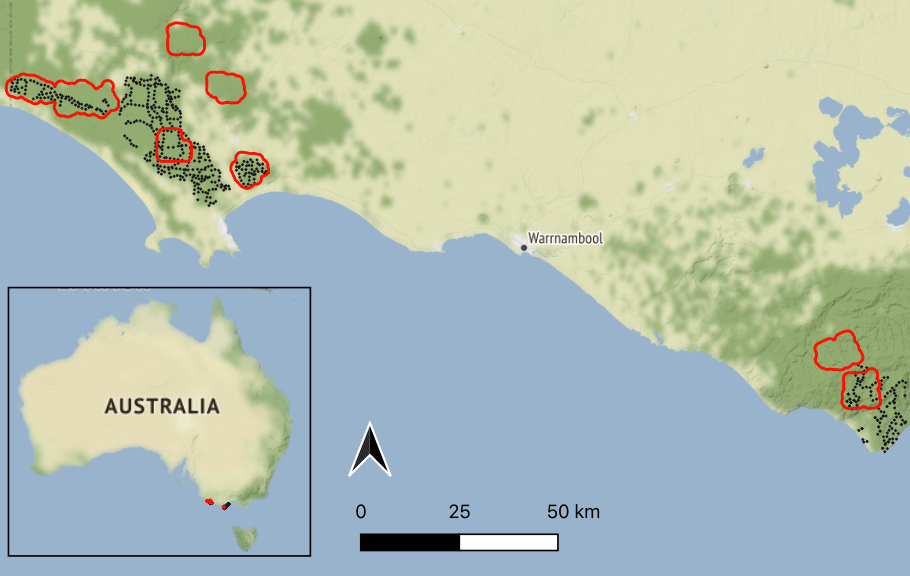
\includegraphics[width=1\linewidth]{figure/map_density} 

}

\caption{Locations of our eight study landscapes in south-west Victoria, Australia (red outlines). Note the two Lower Glenelg National Park landscapes in the far west are shown as one but are separated by a river (which the poison-baits closely follow along the southern bank). Locations of fox poison bait stations are denoted by black dots. The Glenelg region is to the west and Otway region to the east. Native vegetation is indicated by dark green, with hill shading. \textit{Map tiles by Stamen Design, under CC BY 3.0, map data by OpenStreetMap, under CC BY SA.}}\label{fig:density-map}
\end{figure}
\newpage

\hypertarget{results-2}{%
\section{Results}\label{results-2}}

\hypertarget{fox-occurrence}{%
\subsection{Fox occurrence}\label{fox-occurrence}}

In the Glenelg region, there was a clear difference in fox occurrence between paired impact (poison baited) and non-impact landscapes for replicates 1 and 3, but only a marginal difference for replicate 2 (Fig. \ref{fig:foxplot}). In the Otway region, the probability fox occurrence increased by 22\% in the non-impact landscape, and decreased by 43\% in the impact landscape over the three years (occurrence probability averaged at each camera-trap in the landscape). Fox occurrence in the Otway region was generally lower than the Glenelg region, with less fine-scale spatial variation. For example, fox occurrence was predicted to be spatially consistent across the entire Otway region in 2018 (Fig. \ref{fig:foxplot}). Proportion of camera-traps foxes were detected on per landscape are shown in Table \ref{tab:tab-dates}; fox model summaries and spatial standard error estimates are presented in Appendix \ref{density-app-fox}.

\hypertarget{feral-cats-in-the-glenelg-region}{%
\subsection{Feral cats in the Glenelg region}\label{feral-cats-in-the-glenelg-region}}

Across the six landscapes in the Glenelg region, we recorded 251 cat detections from 32,232 camera-trap nights (Table \ref{tab:density-stats}). We were able to identify 64\% of cat detections to the individual level; a total of 67 cats (6 -- 13 individuals per landscape). The exponential detector function was supported over the half-normal function (Table \ref{tab:density-aic-g-1}). The null model was more strongly supported than models with vegetation impacts on cat density and/or linear time trends on \emph{g}\textsubscript{0} (Table \ref{tab:density-aic-g-2}).

At a fine spatial scale, the model with a linear relationship between fox occurrence and cat density was strongly supported (AIC\textsubscript{c} 4.26 better than the null; Table \ref{tab:density-aic-g-3}). It indicated that cat density declined as fox occurrence probabilities increased (-0.32; 95\% CI: -0.57 - -0.07; Fig. \ref{fig:dcor}). There was no evidence of an impact of fox occurrence on cat detectability (Table \ref{tab:density-aic-g-3}). Regression splines added additional model parameters without changing predictions (Fig. \ref{fig:dcor}), and so, all nonlinear models ranked below their linear counterparts (Table \ref{tab:density-aic-g-3}).

Our hypothesis that cat density would be higher in landscapes with fox control was supported for the first and third replicate pairs: estimated cat densities were 2.5 (95\% CI: 1.5 - 4.2) and 3.7 (95\% CI: 1.4 - 9.5) times higher in the impact landscape than the paired non-impact landscape, respectively (Fig. \ref{fig:diffg}). There was no difference in density between landscape pairs in the second spatial replicate (Fig. \ref{fig:diffg}). At the landscape level, there was some evidence that cat detectability was affected by fox occurrence; however the AIC\textsubscript{c} score was only 0.95 units better than the constant detectability model (Table \ref{tab:density-aic-g-4}) and the estimated effects were weak with high uncertainty. This model estimated the detectability of cats in their activity centre (\emph{g}\textsubscript{0}) to increase with the probability of fox occurrence (0.24; 95\% CI: -0.32 - 0.80), as did sigma (0.13; 95\% CI: -0.14 - 0.41).

\hypertarget{feral-cats-in-the-otway-region}{%
\subsection{Feral cats in the Otway region}\label{feral-cats-in-the-otway-region}}

In the Otway region, we recorded 970 cat detections from 36,272 camera-trap nights (Table \ref{tab:density-stats}). We were able to identify 53\% of cat detections to the individual level; a total of 93 cats (20 -- 30 individuals per landscape). The exponential detector function was strongly supported over the half-normal function (Table \ref{tab:density-aic-o-1}). The null model was more strongly supported than the models with vegetation impacts on cat density, as well as camera-trap model and linear time trends on \emph{g}\textsubscript{0} (Table \ref{tab:density-aic-o-2}).

There was some evidence that cat density was negatively correlated with fox occurrence at a fine spatial scale: the two top-ranked models included a linear and a non-linear effect of fox occurrence on cat density, respectively; however, a model without a fox occurrence term received similar support (dAIC\textsubscript{c} = 0.80; Table \ref{tab:density-aic-o-3}). The 95\% confidence interval around the linear coefficient from the top-ranked model marginally overlapped zero (-0.26; 95\% CI: -0.55 - 0.02) indicating that cat density declined as fox occurrence probabilities increased in the Otways at a similar rate to Glenelg, but with slightly greater uncertainty (Fig. \ref{fig:dcor}). However, the equivalent nonlinear model predicted that cat density only declined (at a steeper rate) in the mid-high range of fox occurrence probability (Fig. \ref{fig:dcor}). Equivalent pairs of linear model and nonlinear models were indistinguishable based on AIC\textsubscript{c} scores (Table \ref{tab:density-aic-o-3}). There was also strong support for an effect of fox occurrence on cat detectability at a fine spatial scale (Fig. \ref{fig:detcor}; Table \ref{tab:density-aic-o-4}). Where fox occurrence was higher, cats were less detectable in their activity centres (i.e., negative association with \emph{g}\textsubscript{0}; -0.69; 95\% CI: -1.11 - -0.27; Fig. \ref{fig:detcor}a) and ranged further (i.e., positive association with sigma; coefficient 0.30; 95\% CI: 0.13 - 0.47; Fig. \ref{fig:detcor}b). The equivalent nonlinear model predicted detectability changes to have occurred only in the low-mid range of fox occurrence (Fig. \ref{fig:detcor}).

Our hypothesis that cat density in the impact landscape would increase relative to the non-impact landscape with fox control was supported in 2019, but not 2018. Cat density was estimated to be lower in the impact than non-impact landscape prior to fox-baiting (i.e., in 2017; Fig. \ref{fig:diffo}). In 2018, cat density decreased in the non-impact landscape and increased in the impact landscape, converging to near-identical density estimates. These patterns continued at the same rate into 2019, with cat density estimated to be higher in the impact landscape than the non-impact landscape. There was not statistical evidence that the difference between cat density in landscape pair had changed from 2017 to 2018 as these 83\% confidence intervals overlapped, but there was weak statistical evidence of an relative increase in cat density in the impact landscape from 2017 to 2019 as these 83\% confidence intervals narrowly avoided overlap (Fig. \ref{fig:diffo}b). Like the fine-scale model, there was strong evidence that cat detectability was impacted by fox occurrence (Table \ref{tab:density-aic-o-4}).

\newpage

\(~\)

\(~\)

\(~\)
\begin{figure}

{\centering 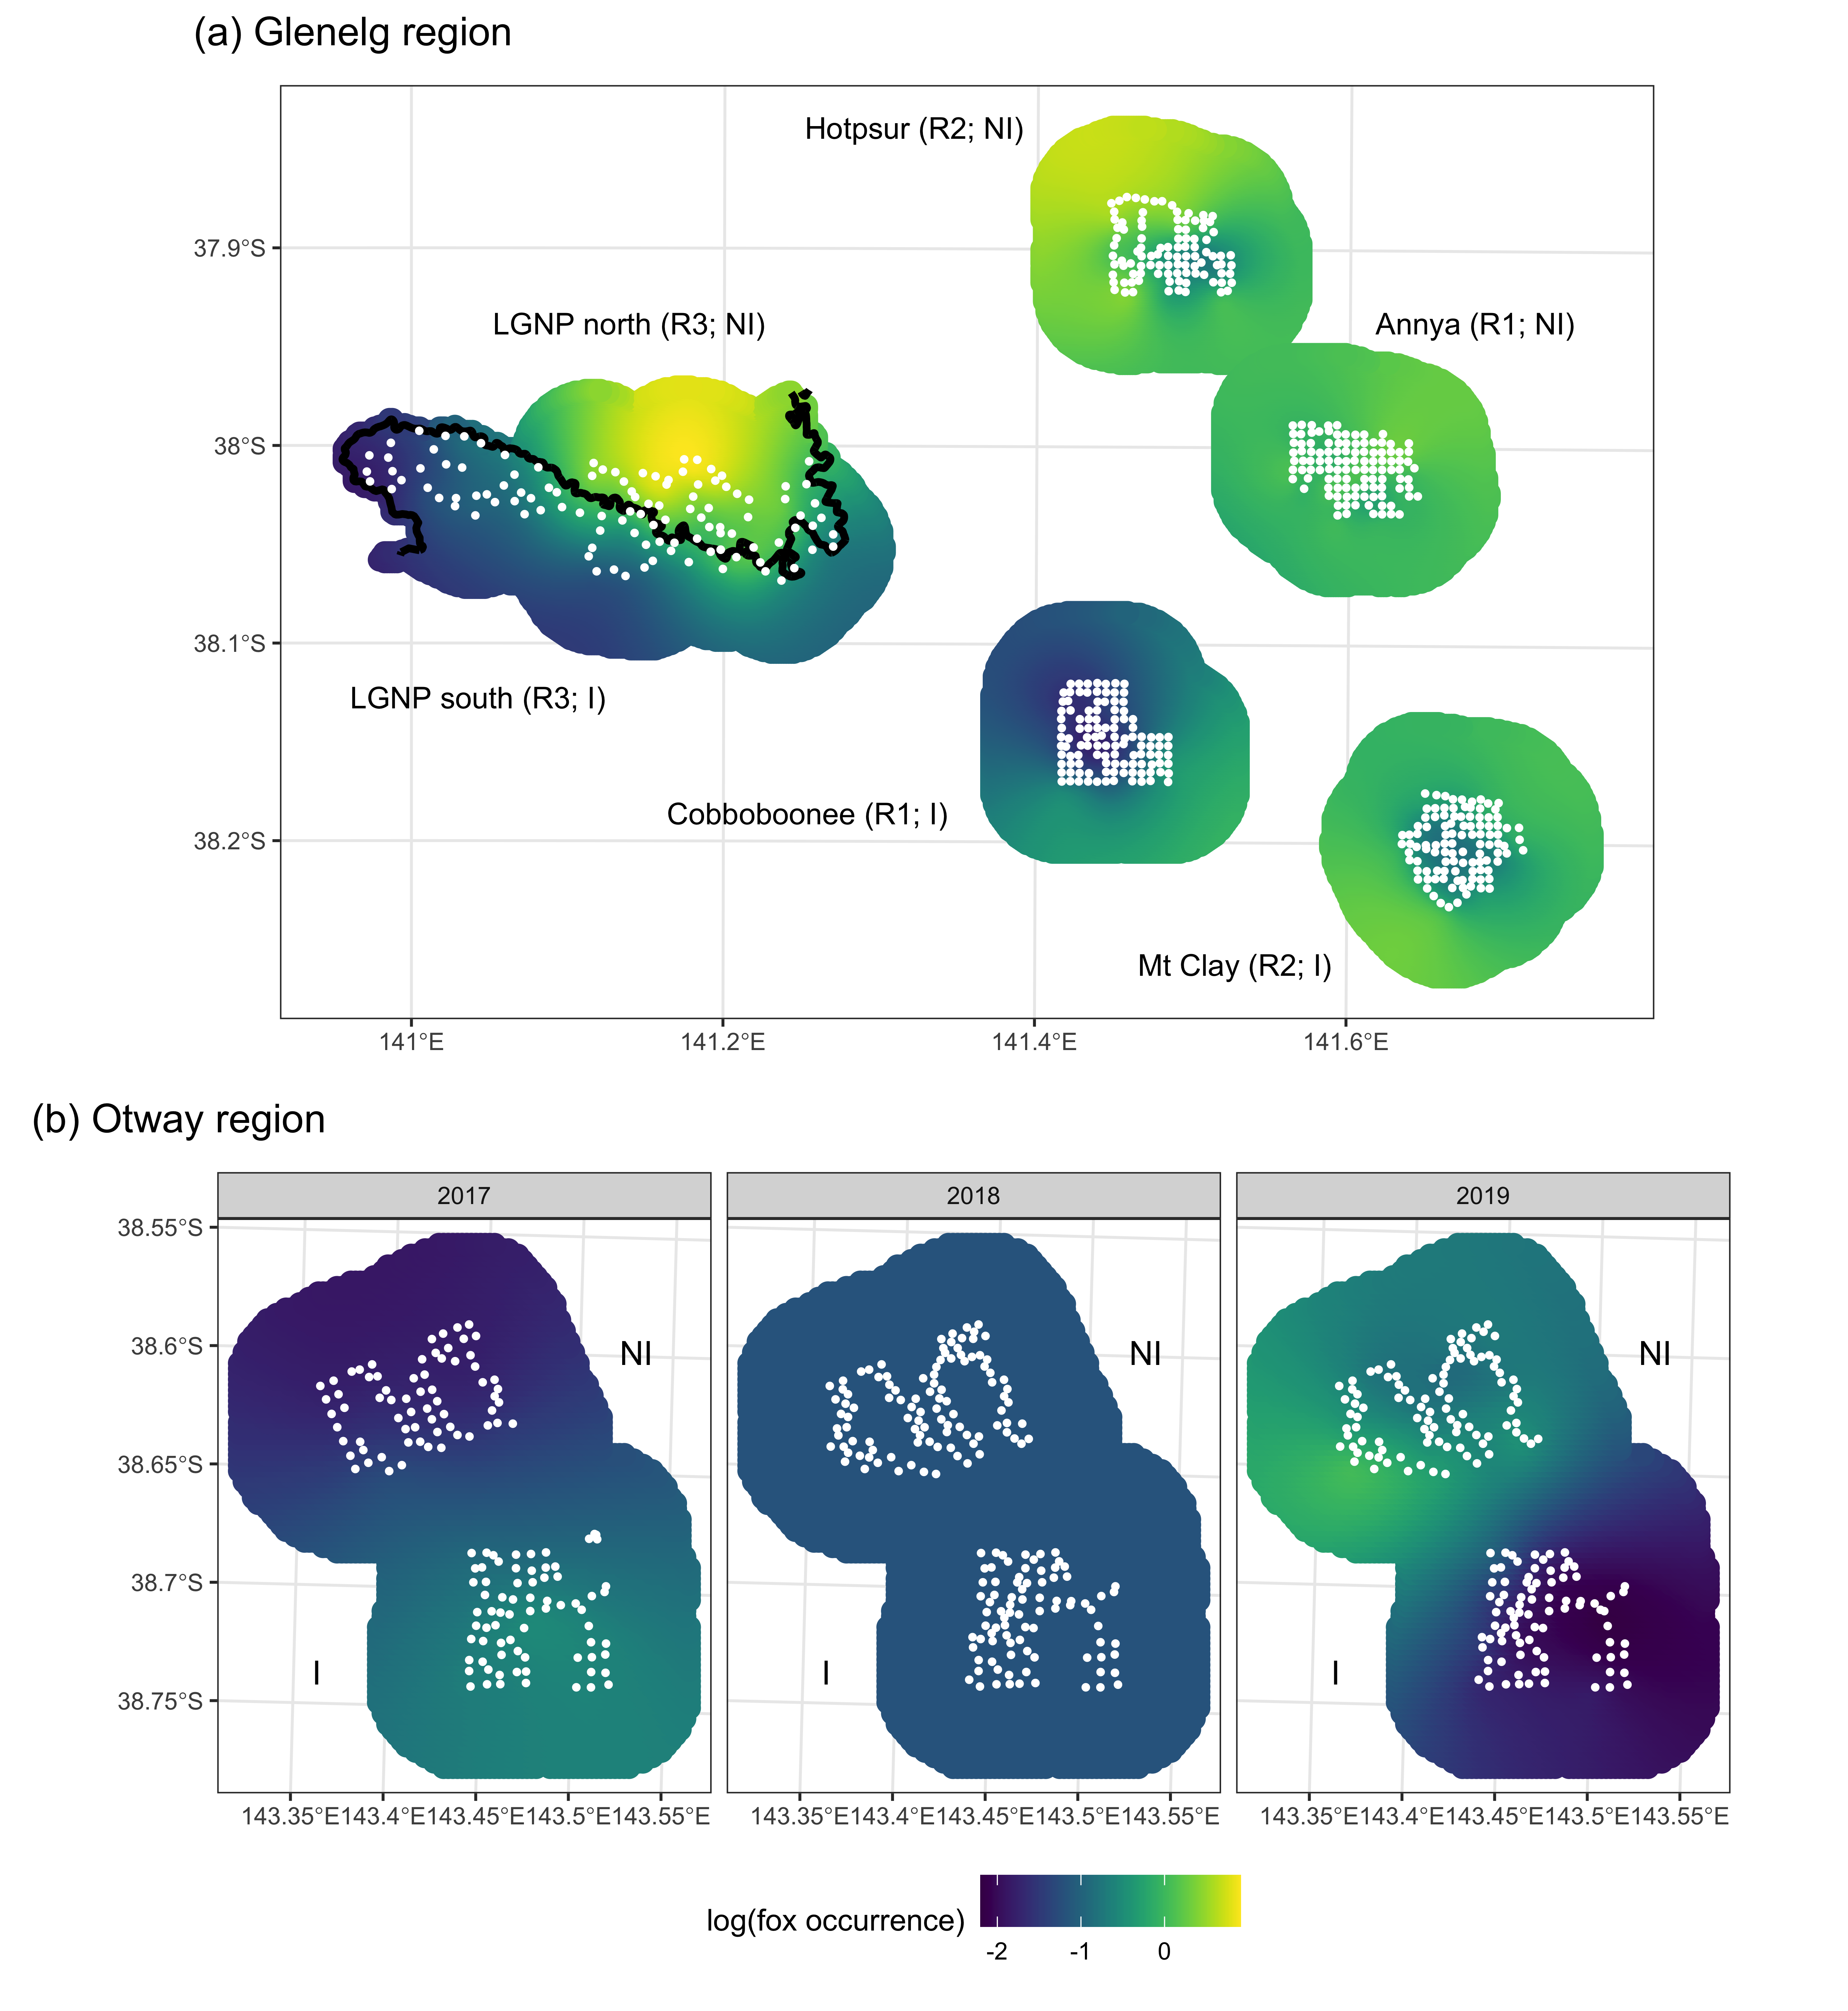
\includegraphics[width=1\linewidth]{figure/fox_occ_map} 

}

\caption{Predicted red fox \textit{Vulpes vulpes} occurrence derived from generalised additive models within each impact (I) and paired non-impact (NI) landscape in the Glenelg (a) and Otway (b) regions, Australia. White dots represent camera-trap sites. Predicted fox occurrence on the natural logarithmic scale was used as a predictor of feral cat Felis catus density in the spatial mark-resight models.}\label{fig:foxplot}
\end{figure}
\newpage

\(~\)

\(~\)

\(~\)
\begin{figure}

{\centering 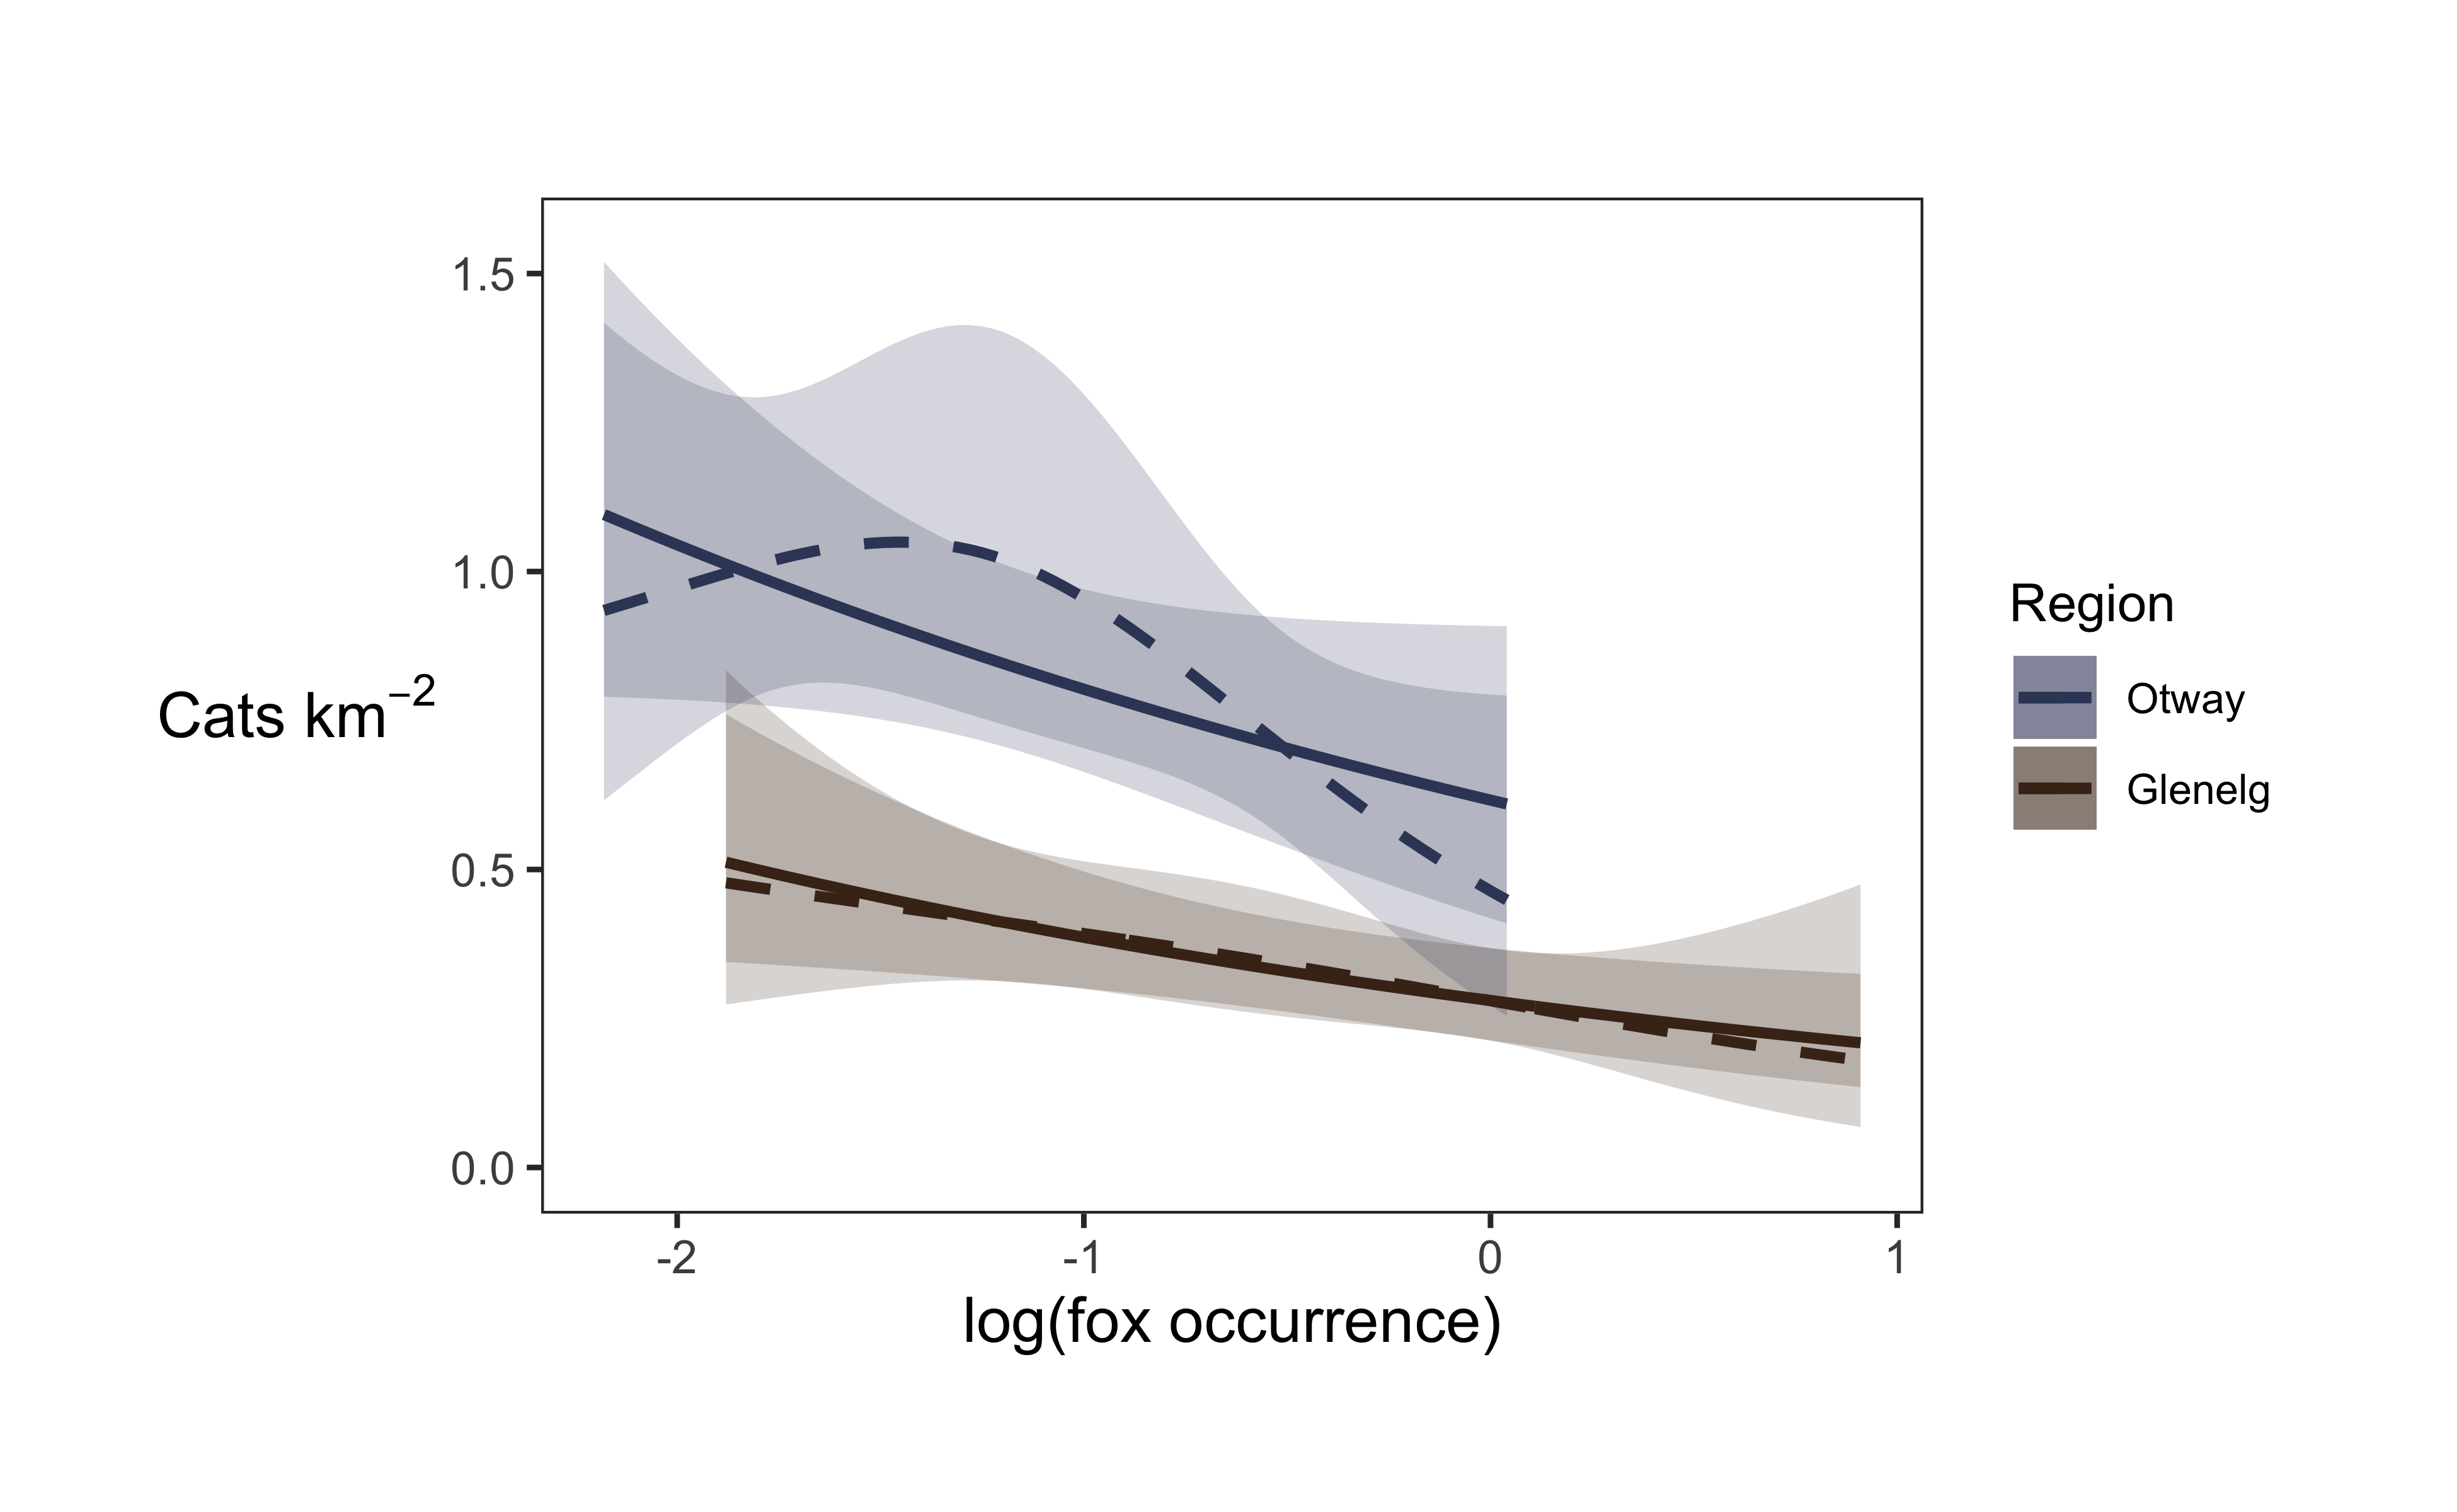
\includegraphics[width=1\linewidth]{figure/foxD_600dpi} 

}

\caption{Linear (solid lines) and nonlinear (dashed lines) models predicted that feral cat \textit{Felis catus} density increased with declining probability of red fox \textit{Vulpes vulpes} occurrence probability (log-transformed) in the Glenelg and Otway regions, Australia. Shaded areas indicate 95\% confidence intervals. In both regions, the top-ranked models included a linear, negative association between feral cat density and fox occurrence probability; these models were ranked more highly than their nonlinear counterparts in terms of Akaike Information Criterion scores. However, there was not strong statistical evidence for this association in the Otway region: the 95\% confidence intervals of the coefficient for the linear model narrowly overlapped zero, and a model without this association performed similarly well in terms of Akaike Information Criterion scores.}\label{fig:dcor}
\end{figure}
\newpage

\(~\)

\(~\)

\(~\)
\begin{figure}

{\centering 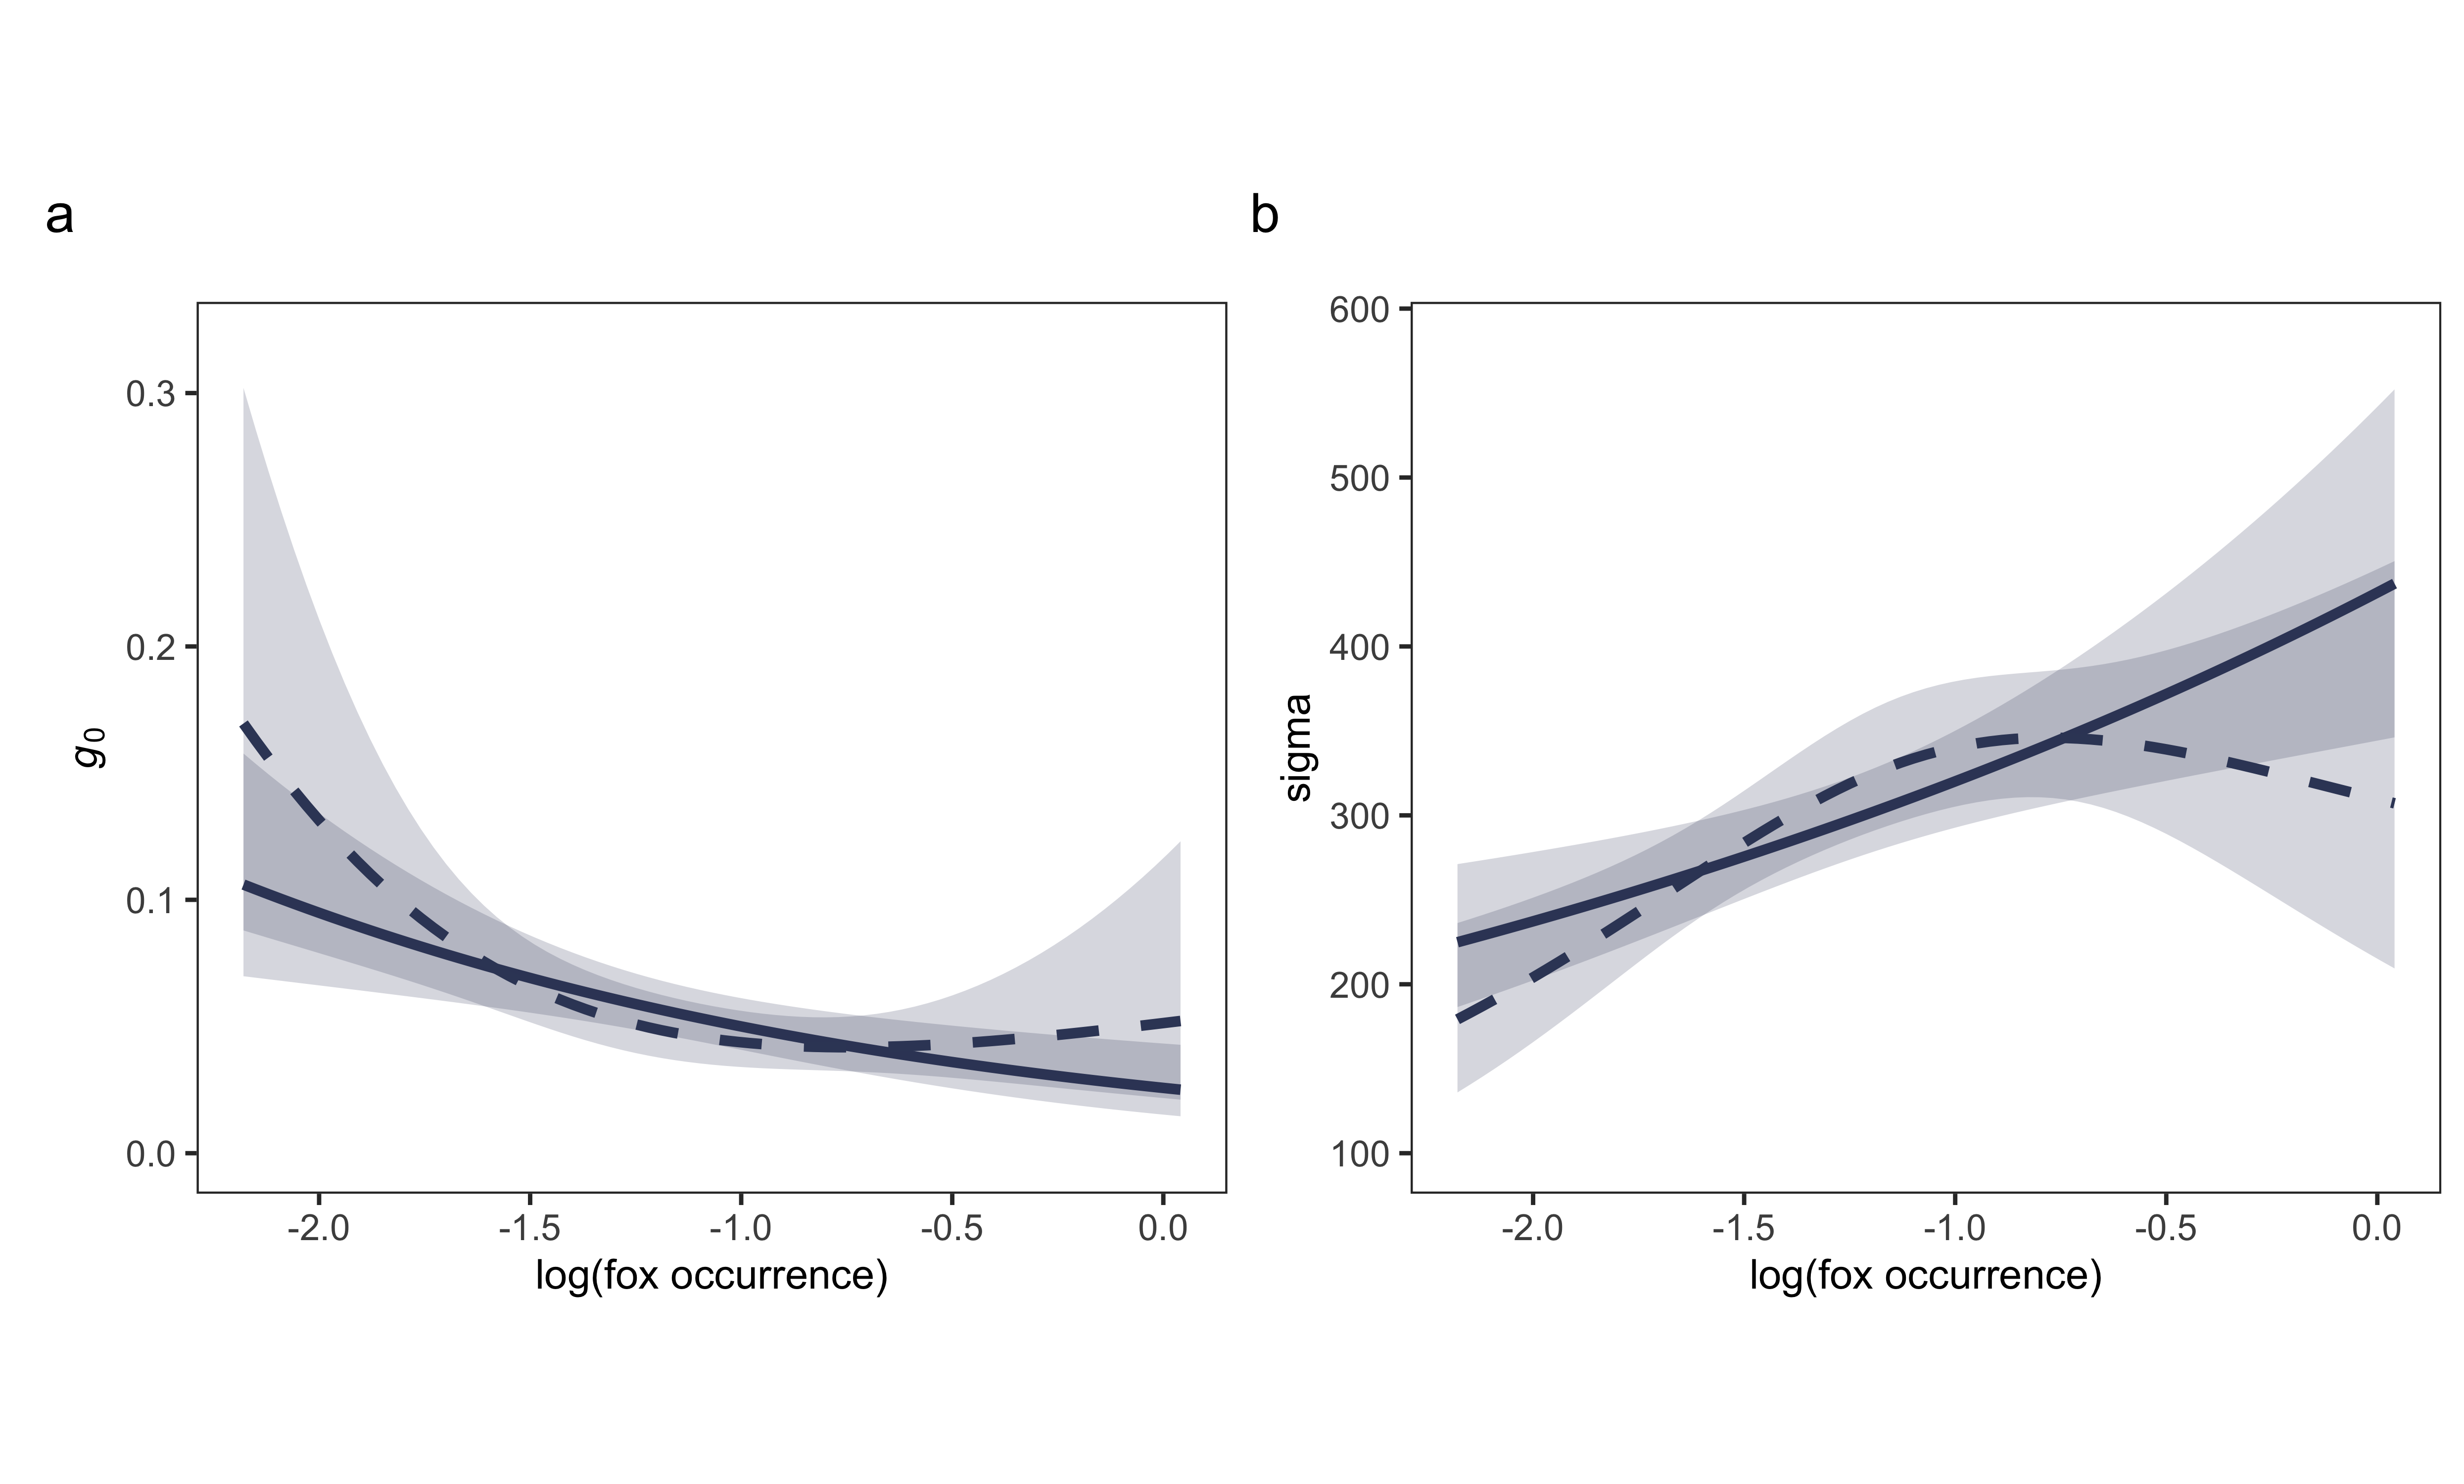
\includegraphics[width=1\linewidth]{figure/foxDet_otways_600dpi} 

}

\caption{Linear (solid lines) and nonlinear (dashed lines) models of feral cat \textit{Felis catus} detectability as a function of log-scaled red fox \textit{Vulpes vulpes} occurrence in the Otway region, Australia. The probability of detecting a feral cat in its activity centre per 24-hour occasion (\textit{g}\textsubscript{0}) decreased with the probability of fox occurrence (a), while sigma (which is related to home range size; exponential detection function) increased (b). Shaded areas indicate 95\% confidence intervals.}\label{fig:detcor}
\end{figure}
\newpage

\(~\)

\(~\)

\(~\)
\begin{figure}

{\centering 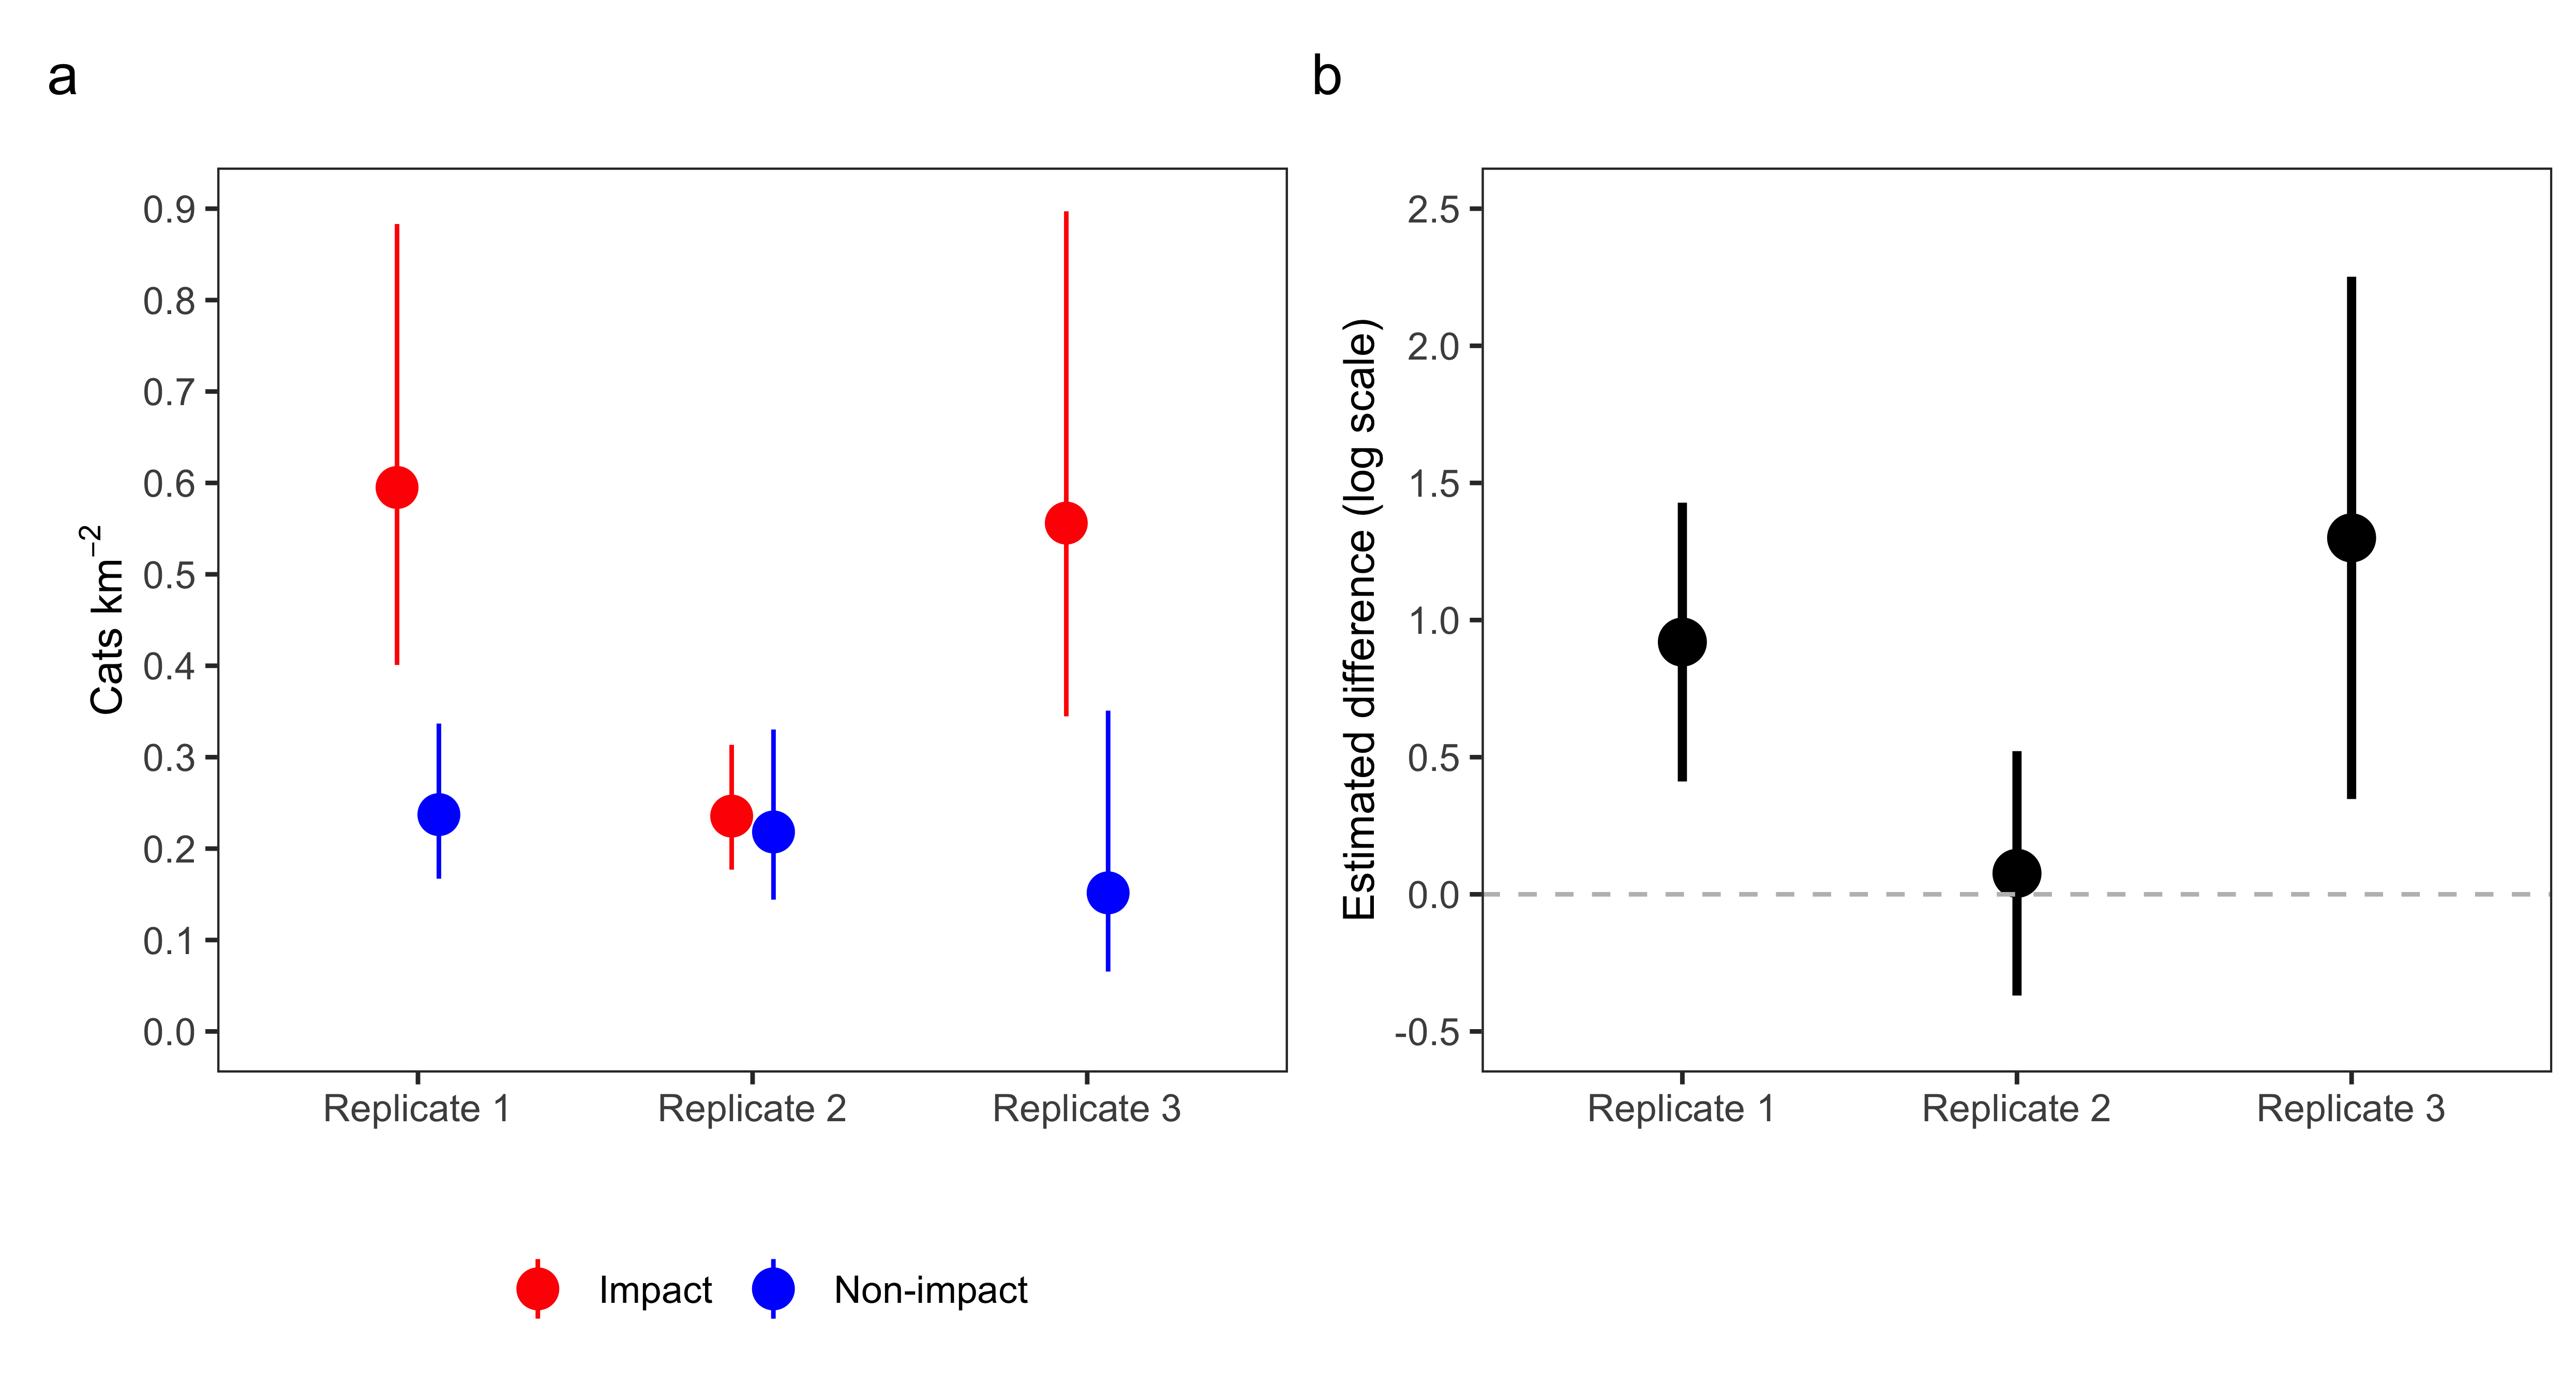
\includegraphics[width=1\linewidth]{figure/glenelg_estimates_600dpi} 

}

\caption{Results of the spatially replicated Control-Impact analysis of feral cat \textit{Felis catus} density in response to long-term fox control in the Glenelg region, Australia. Poison baiting for foxes \textit{Vulpes vulpes} had been conducted continuously in the impact landscapes for more than 13 years at the time of the first two replicate surveys (2018) and 16 years for the third replicate (2021). Panel A presents cat density estimates with 95\% confidence intervals for each landscape derived from spatial mark-resight models. Panel B presents estimates of difference in cat density between landscape pairs (impact landscape relative to the paired non-impact landscape) for each replicate. 95\% confidence intervals which do not overlap 0 (grey dashed line) demonstrate statistical evidence (p-value < 0.05) that cat density was higher in the impact landscape relative to the associated non-impact landscape, which was the case for the first (Annya and Cobboboonee) and third (Lower Glenelg National Park North and South), but not the second replicate (Hotspur and Mt Clay).}\label{fig:diffg}
\end{figure}
\newpage

\(~\)

\(~\)

\(~\)
\begin{figure}

{\centering 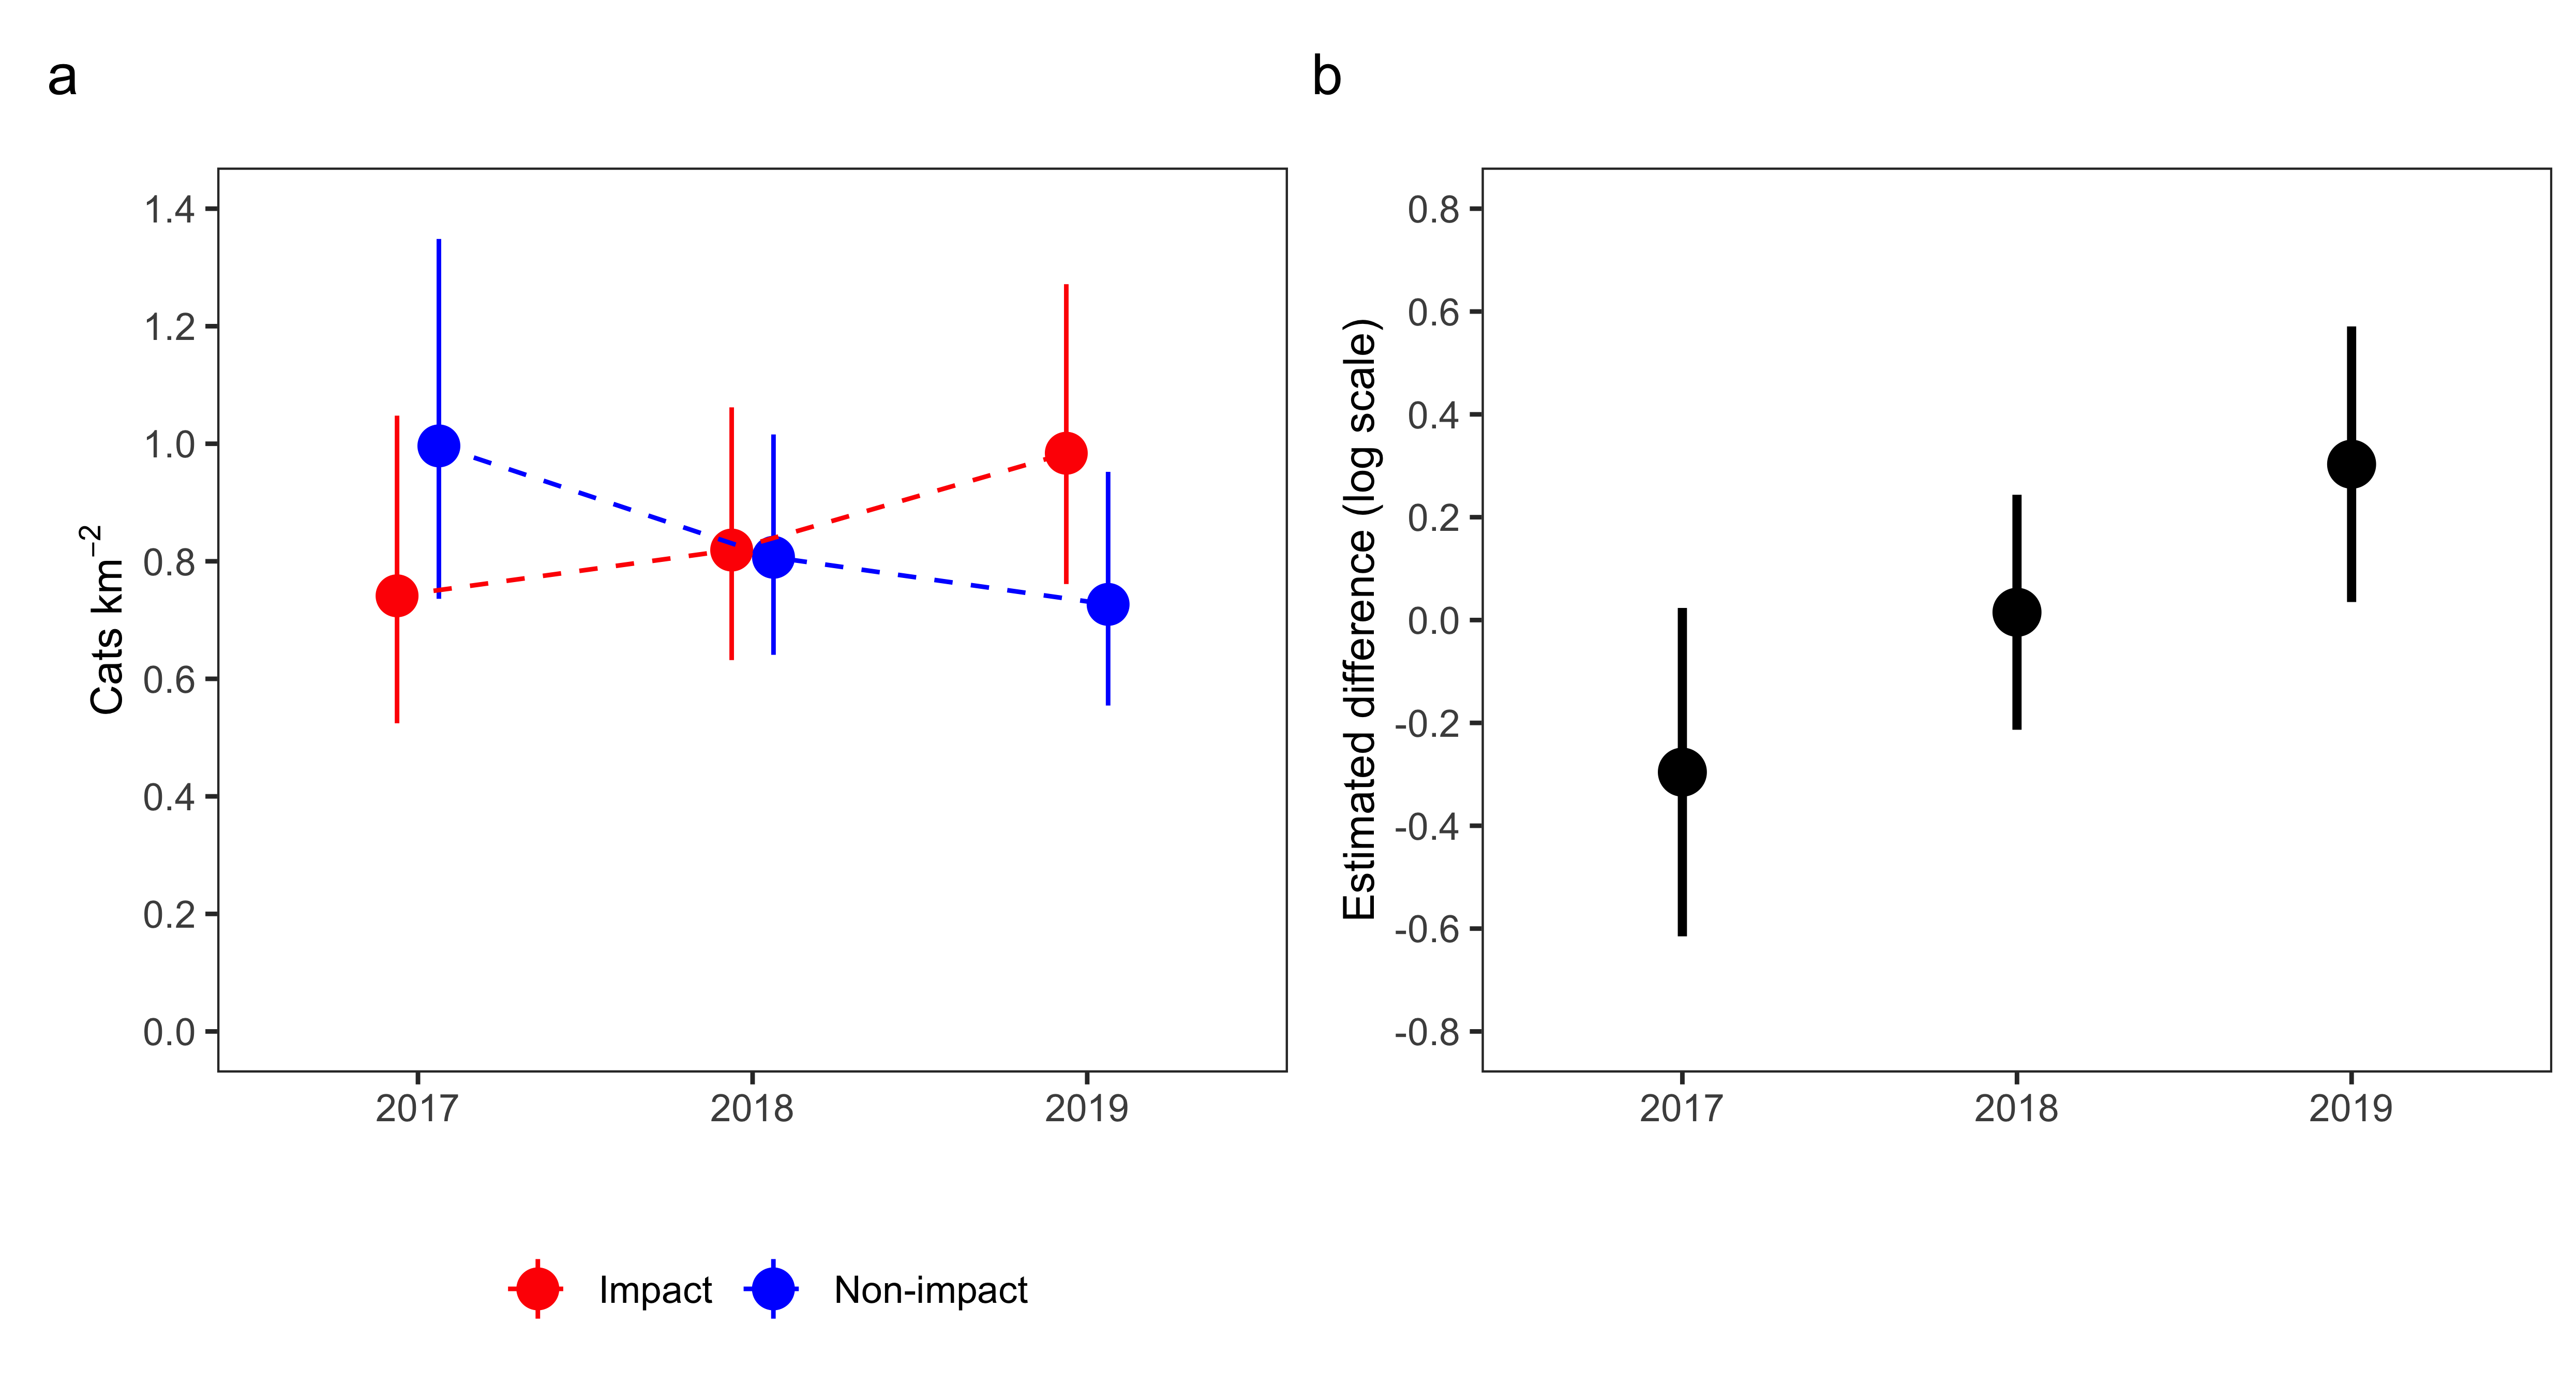
\includegraphics[width=1\linewidth]{figure/otways_estimates_600dpi} 

}

\caption{Results of the Before-After Control-Impact Paired-Series analysis of feral cat \textit{Felis catus} density in response to fox control in the Otway Ranges, Australia. In 2017, surveys were conducted approximately two months before lethal red fox \textit{Vulpes vulpes} control commenced in the impact landscape (although fox control ceased for six months just after the 2018 survey started, resuming again five months prior to the 2019 survey). Panel A presents cat density estimates with 95\% confidence intervals for each landscape survey derived from spatial mark-resight models. Panel B presents estimates of the difference (on the natural logarithmic scale) between landscape pairs in each survey year (impact landscape relative to the non-impact landscape) with 83\% confidence intervals. Overlap between 83\% confidence intervals in successive years (visualised horizontally; b) is used to assess evidence of a change in the relative cat density between landscape pairs; no overlap indicates a p-value less than 0.05. There was not statistical evidence of a change in cat density from 2017 - 2018, but there was weak evidence for a change from 2017 to 2019 (these 83\% confidence intervals narrowly avoid overlap).}\label{fig:diffo}
\end{figure}
\newpage

\hypertarget{discussion-2}{%
\section{Discussion}\label{discussion-2}}

Our study is one of the first to provide replicated, experimental evidence that dominant predator suppression is associated with higher mesopredator densities. Our study provides two lines of evidence that foxes can exert top-down control on feral cats in the forests of south-eastern Australia: feral cat density was (1) higher where fine-scale fox occurrence probability was lowest (although this association was uncertain in the Otway region), and (2) commonly higher in landscapes where fox control occurred. This is concerning because targeted fox control is a widely used conservation strategy; this unintended consequence could dampen benefits to native prey and even further threaten these species (Courchamp, Langlais, \& Sugihara 1999; Wayne \emph{et al.} 2017). However, as our findings highlight, mesopredator release of cats following fox control depends on the degree of fox suppression. More broadly, our study illustrates how correlative and experimental approaches provide complementary lines of evidence when investigating interactions between predator species, and the importance of disentangling changes in population density from changes in detectability.

We were able to exploit a gradient in fox occurrence probability caused by lethal control to investigate associations between cat density and fox occurrence at a fine spatial scale across two separate regions. At this scale, we observed a consistently negative association between cat density and fox occurrence probabilities, supporting our first hypothesis. While AICc scores indicated that cat density had negative associations with fox occurrence probabilities across both regions, only this association in the the Glenelg region was statistically significant (95\% confidence intervals for this coefficient narrowly overlapped zero in the Otway region). Negative spatial associations between species may simply reflect differences in niche preference rather than exclusion or avoidance, although is less likely in our case given we observed the relationship across an artificial gradient of fox occurrence probability caused by lethal control. Cats may respond more closely to fox occurrence at broader spatial scales (i.e., the landscape level), or to fox activity (i.e., counts of detections rather than presence-absence). This is worth future investigation, particularly as simultaneously estimating fox density from camera-trap surveys remains unreliable due to the inability to identify individual foxes from photographs (Güthlin, Storch, \& Küchenhoff 2014).

There is contention around whether linear regression is appropriate for investigating correlations between different predator species, as subordinate predators may only be suppressed when dominant predator abundance is high (Johnson \& VanDerWal 2009; Letnic \emph{et al.} 2011). We found no evidence of non-linear associations between foxes and cats in the Glenelg region, while linear and non-linear models performed equally well in the Otway region. Non-linear models in the Otway region predicted that cat density declined only in the mid-high range of fox occurrence, while behavioural changes were seen in the low-mid range of fox occurrence. Perhaps cats can successfully avoid foxes through behavioural change where foxes are rare, but this is ineffective where foxes are common. This could explain the lack of evidence for foxes impacting cat detectability in the Glenelg region where fox occupancy is relatively high. Alternatively, behavioural changes may be untenable for cats in the Glenelg region because small mammal abundance is relatively low (M.Rees, unpublished data) and fox avoidance strategies likely come at the expense of hunting success (Sih 1980; Wilson \emph{et al.} 2010).

Where fox occurrence was higher in the Otway Ranges, cats were less detectable in their activity centres and ranged further (Fig. \ref{fig:detcor}). Low detectability is likely to correlate with fewer dominant predator encounters, and has been observed in other predator interaction studies (e.g., Lombardi \emph{et al.} 2017). An increase in cat ranging behaviour (sigma) with fox control supports observations made by Molsher \emph{et al.} (2017) using telemetry, and may reflect a direct avoidance strategy. Animal movement rates are expected to increase in response to unpredictable threats (Riotte-Lambert \& Matthiopoulos 2020). Alternatively, cats may consider foxes predictable and avoid locations they frequent, thus having to range further to obtain the same amount of food resources. In a similar forest habitat, Buckmaster (2012) observed large `holes' in the home range of each GPS-collared cat; they confirmed that this was not due to an absence of prey and hypothesised it was due to dominant predator avoidance. Further, in similar forest habitat without any foxes or dingoes, cats tend to have compact home ranges within which their intensity of use is reasonably uniform, suggesting this to be an optimal strategy for cats (Hamer \emph{et al.} 2021b). A more extended home range used in a patchy fashion, might therefore be a suboptimal strategy for cats. Regardless of the cause, variation in mesopredator detectability and movement rates with dominant predator populations has serious implications for the interpretation of studies that simply compare relative abundance indices or spatial overlap of predator species without disentangling behaviour and detectability from density (Efford \& Dawson 2012; Neilson \emph{et al.} 2018; Stewart \emph{et al.} 2018; Broadley \emph{et al.} 2019).

In the Glenelg region where fox-baiting had occurred for more than 13 years, feral cat density was considerably higher in two out of three distinct landscapes than in similar, unbaited landscapes. The outlier is most likely due to limited suppression of foxes at Mt Clay despite ongoing fox control (Fig. \ref{fig:foxplot}a). Mt Clay is a small forest block surrounded entirely by unbaited farmland; simulation modelling indicates that the size of the baited area is a key driver of the degree of reduction in the fox population (Hradsky \emph{et al.} 2019; Francis, Robley, \& Hradsky 2020).

In the Otway region, we observed seemingly opposing patterns of fox occurrence probabilities in the impact and non-impact landscapes over time (Fig. \ref{fig:foxplot}b). We are unsure what drove the increase in fox occurrence probability in the non-impact landscape and whether it was related to fox control in the nearby impact landscape, although this provides an explanation as to why cat density increased in the non-impact site (Fig. \ref{fig:diffo}a). The effects observed in our BACIPS study are therefore only partly due to mesopredator release in the strict sense (i.e., due to fox suppression), although demonstrate reciprocity in responses of cats to both increases and declines in foxes, which is rarely observed (Alston \emph{et al.} 2019). Perhaps changes in the non-impact landscape were due to changes in prey availability, although we do not expect large fluctuations in prey here given the low seasonality and consistent climatic conditions relative to other parts of the country. Studies of fox-cat (and other intraguild predator) interactions often use the presence of a management program as a proxy for dominant predator suppression (e.g., Hunter \emph{et al.} 2018). Our findings strongly indicate the need to directly measure the dominant predator population in order to reliably interpret the responses of subordinate species (Salo \emph{et al.} 2010).

In the Otway region, we observed a weak---but increasing---effect of fox control on cat density, to be expected from a recently commenced fox-baiting program. We consider two possible explanations for the weaker response of cats to fox control in the Otway Ranges than the Glenelg region. Firstly, the short duration of baiting in the Otway region may mean that changes in adult cat density are yet to fully manifest. We found some evidence for a sequential response of first, a relaxation of behavioural mediation - potentially improving hunting success and recruitment rates, may in-turn cause a subsequent increase in cat density. Additionally, foxes are more likely to be effective at killing younger cats which are more vulnerable, and so may have a greater impact on cat recruitment rates rather than the adult popultion. Further, cats may also respond to an increase in shared prey availability following fox suppression (Stobo-Wilson \emph{et al.} 2020a). A time-lagged release of cats following fox control would explain eruptions and subsequent crashes commonly observed in shared mammalian prey populations two to ten years following fox control commencement (Duncan \emph{et al.} 2020).

Secondly, foxes may have a weak suppressive effect on cats in the highly productive Otway region. Fox occurrence (Fig. \ref{fig:foxplot}) and density was already relatively low prior to fox control in the Otways (Le Pla \emph{et al.} 2022), limiting their suppressive effects on cats. Additionally, competition theory predicts competitive interactions to be weaker with high prey availability; there is likely less imperative for foxes to be aggressive towards cats when there is enough food to share (Johnson \& VanDerWal 2009; Greenville \emph{et al.} 2014). On the other hand, foxes may have a higher capacity to maintain vigilance against cats when they are not food stressed, and top-down control from dominant predators may be the only limiting factor of this generalist mesopredator in resource-rich environments (Oksanen \& Oksanen 2000; Elmhagen \& Rushton 2007; Feit, Feit, \& Letnic 2019). Prey availability is likely a strong mediator of mesopredator release, although it remains unclear whether mesopredator release would be stronger where prey availability is low or high---severely limiting our ability to predict mesopredator release across different landscapes.

Perhaps the most obvious omission in our study is therefore trends in prey. It is difficult to ascertain whether mesopredator release was stronger in the Glenelg or Otway regions because of the different length of times foxes had been controlled for, although the negative associations between cat density and fox occurrence was only marginally stronger in the Glenelg region than the Otway. Teasing apart the relative importance of fox and prey associations with feral cat density will be important for both understanding the mechanisms, and accurately predicting mesopredator release of cats across different landscapes. Another limitation of our approach is that uncertainty from our fox occurrence models was not propagated into the spatial mark-resight models. A full Bayesian integration of the fox occurrence analysis and the spatial mark-resight model to address this is not yet implemented. The development of open population spatial mark-resight models would also improve parameter estimates for repeat surveys in landscapes.

Nevertheless, our study is among the very few which have used a direct measure of density to test mesopredator release. Previous studies have mostly used live capture-rates to infer population density, without accounting for behavioural or detectability changes (e.g., Arjo \emph{et al.} 2007; Karki, Gese, \& Klavetter 2007; Thompson \& Gese 2007; Berger, Gese, \& Berger 2008; Jones, Van Vuren, \& Crooks 2008). Contention about mesopredator release has centred on such methods (Hayward \emph{et al.} 2015), as well as unaccounted species interactions in complex predator guilds (Levi \& Wilmers 2012; Jachowski \emph{et al.} 2020). In contrast, our study tests the mesopredator release theory using a combined behavioural and numerical approach, in a system with a simplified carnivore guild. Further replication of our approach in new landscapes, as well as explictly accounting for prey species or landscape productivity is a priority for improving understanding of mesopredator release. However, it is extremely difficult to find comparable landscapes and as we have shown, binary variables for predator control overlook important ecological nuance. Testing associations between dominant and subordinate predators across wider gradients of productivity and predator control effort may even provide more accurate inference than additional replicated experiments with traditional designs (Kreyling \emph{et al.} 2018), and could be achieved using data already collected.

The results of our study may explain why pest management that only targets foxes---one of the most prevalent conservation actions in Australia---does not consistently improve native prey persistence (Dexter \& Murray 2009; Robley \emph{et al.} 2014; Wayne \emph{et al.} 2017; Lindenmayer \emph{et al.} 2018; Duncan \emph{et al.} 2020). More evidence is required to understand the circumstances in which lethal fox control increases cat density, particularly the role of baseline fox and prey densities. A more integrated approach to invasive predator management, where foxes and cats are simultaneously or otherwise optimally controlled could substantially improve biodiversity outcomes (Risbey \emph{et al.} 2000; Comer \emph{et al.} 2020). If this is not feasible, changes in invasive mesopredator density and the outcomes for native prey species should be closely monitored as part of any control program for invasive dominant predators, with triggers for ceasing dominant predator control or commencing integrated management if single-species control proves counterproductive for the conservation of threatened prey species.

\hypertarget{diel}{%
\chapter{Spatial variation in predator diel activity patterns --- feral cats avoid red foxes in time not space}\label{diel}}

\hypertarget{abstract-3}{%
\section*{Abstract}\label{abstract-3}}
\addcontentsline{toc}{section}{Abstract}

Understanding the constraints dominant predators impose on subordinate species is important for anticipating outcomes of predator management. Subordinate predators may avoid dominant predators in time or space, making it difficult to fully quantify antipredator behaviours unless joint spatiotemporal analyses are used.

Here, we tested whether an invasive top predator (red fox \emph{Vulpes vulpes}) alters the spatiotemporal activity of an invasive subordinate predator (feral cat \emph{Felis catus}). We surveyed both species using 3,667 camera-trap deployments across two regions of south-eastern Australia; foxes were poison-baited in some landscapes within each region. The simple predator guild allowed sharp focus on how experimental gradients in fox activity affected feral cat behaviour. We used generalised additive models to quantify the overall activity of each species across space and throughout the daily cycle.

Foxes and cats had similar diel activity patterns when averaged across all sites; however, there was important differentiation at a finer scale. When localised fox activity was high, cats did not reduce their overall activity but shifted diel patterns. In dry vegetation types, foxes were largely nocturnal and, at sites where foxes were more active, cats were more diurnal. In contrast, in wet forests, overall fox activity was lower and consistent throughout the daily cycle; at sites where foxes were more active, cats were more nocturnal (avoiding dawn in particular). Changes in cat diel activity patterns may facilitate spatial coexistence between these two invasive predators, potentially shifting feral cat impacts onto different native prey.

It is well-appreciated that overall predator activity varies spatially and fluctuates throughout the daily cycle. Our study demonstrates that diel activity patterns also vary across space, likely mediated by both landscape context and fear. Apex predator avoidance appears to be dynamic across landscapes of fear---a key nuance which is overlooked when simply comparing the average activity or spatial overlap between two species.

\newpage

\hypertarget{introduction-3}{%
\section{Introduction}\label{introduction-3}}

Predators shape ecosystems through both predation and the fear of predation (Creel \& Christianson 2008; Ritchie \& Johnson 2009; Allen, Clinchy, \& Zanette 2022). Fear-induced behavioural suppression can be as detrimental to subordinate species as predation itself (Schmitz, Krivan, \& Ovadia 2004; Preisser, Bolnick, \& Benard 2005). These non-consumptive effects of apex predator are expected to be strong drivers of mesopredator behaviour, particularly when resource competition is high (Ritchie \& Johnson 2009). A strengthening or relaxing of antipredator behaviours by mesopredators can have cascading effects across the entire ecosystem: altering population demographics, species interactions, ecological function and human-wildlife coexistence (Brown, Laundré, \& Gurung 1999; Ripple \& Beschta 2004; Estes \emph{et al.} 2011; Gaynor \emph{et al.} 2019; Lamb \emph{et al.} 2020). Hence, understanding how apex predators constrain the behaviour of subordinate species is important to accurately predict the ecosystem-wide consequences of predator management, such as reintroductions or lethal control (Gaynor \emph{et al.} 2021).

Spatial and/or temporal niche partitioning may allow predators to coexist by reducing encounter-rates and resource overlap (Kronfeld-Schor \& Dayan 2003). However, mesopredators may not consistently employ avoidance behaviours because perceived predation risk is temporally and spatially variable, and antipredator behaviours typically involve a trade-off against resource acquisition, such as limiting or relegating activity to suboptimal places or times (Lima \& Dill 1990; Lima \& Bednekoff 1999). Therefore, optimal predator avoidance strategies are likely to vary across heterogeneous landscapes where resource availability (e.g., shelter, food) and perceived predation risks differ (Kauffman \emph{et al.} 2007; Willems \& Hill 2009; McCann, Zollner, \& Gilbert 2017; Wirsing \emph{et al.} 2021). For example, temporal predator avoidance may be preferable over spatial avoidance if food is constantly available throughout the day, and vice versa. These theories are unified under the `ecology of fear' concept (Brown, Laundré, \& Gurung 1999), which has gained increasing attention in recent times (Gaynor \emph{et al.} 2019). Notably, the mesopredator release hypothesis has recently been expanded from increases in mesopredator abundance following apex predator decline (Soulé \emph{et al.} 1988) to also include changes in mesopredator behaviour (Brashares \emph{et al.} 2010).

To accurately quantify avoidance within a predator guild, we first need to understand how the overall activity and diel activity patterns of each species varies `naturally' across landscapes, particularly for species with broad distributions. It is widely recognised that the overall activity of different predator species varies across their distributions, but their diel activity patterns are often assumed to be constant. In this paper, we use the term `overall activity' to refer to the number of `independent' predator detections at a site (offset to account for survey duration; analogous to an activity or abundance index), and `diel activity pattern' to refer to fluctuations in relative activity throughout the 24-hour daily cycle. Overall activity is influenced by predator behaviour, population density and the detection process (Anderson 2001), whereas diel activity patterns are a behavioural trait (less likely to be affected by the detection process, if the survey methodology remains consistent).

Despite modern predator survey technologies providing time-stamped detections, detection times are commonly discarded from analyses, probably because joint modelling of overall activity and diel activity patterns is more complicated. When temporal avoidance is tested, it is usually considered in an ad-hoc fashion, by fitting separate models for spatial and temporal avoidance, or by repeating spatial analyses (e.g., resource selection functions) at different time periods (e.g., Basille \emph{et al.} 2015; Kohl \emph{et al.} 2019; Smith \emph{et al.} 2019). However, discretising the daily cycle into categorical periods (e.g., day and night) introduces bias, assuming animals have complete step-changes in behaviour rather than progressive shifts across the daily cycle. Further, dawn and dusk are particularly important times for many predator species.

Generalised Additive Models (hereafter `GAMs') are increasingly being used to estimate animal diel activity patterns and offer a flexible framework to jointly consider overall activity. GAMs also have other benefits, including smoothing penalties to reduce overfitting, the ability to capture nonlinear interactions between multiple variables with different units, and the ability to share information across categorical variables through hierarchical specifications (Wood 2017; Pedersen \emph{et al.} 2019). However, we are only aware of one study which allowed animal diel activity to interact with predation risk as a continuous variable in a GAM (although without considering overall activity, Cunningham \emph{et al.} 2019).

The red fox \emph{Vulpes vulpes} (hereafter `fox'; \textasciitilde6 kg) and feral cat \emph{Felis catus} (hereafter `cat'; \textasciitilde4 kg) have devastating impacts on native prey throughout their introduced range, implicated in the extinction of \textasciitilde10 and 63 species, respectively (Doherty \emph{et al.} 2016). The impacts of these invasive predators have been particularly extreme on the Australian continent (Woinarski, Burbidge, \& Harrison 2015). Cats are more difficult to manage, and so introduced predator control programs in Australia often target only foxes (particularly through poison-baiting, Reddiex \emph{et al.} 2007). As foxes and cats compete for many of the same resources, there is concern that lethal fox control could cause a mesopredator release (Soulé \emph{et al.} 1988) of feral cats (Glen \& Dickman 2005; Robley \emph{et al.} 2014; Marlow \emph{et al.} 2015a; Doherty \& Ritchie 2017; Wayne \emph{et al.} 2017; Comer \emph{et al.} 2020). There is some evidence that feral cats increase in activity (although highly uncertain, Hunter \emph{et al.} 2018), density (Chapter \ref{density}) and alter their diets and use of space (Molsher \emph{et al.} 2017) in response to fox control. Other studies have investigated potential spatial and temporal interactions between these invasive predators (e.g., Roshier \& Carter 2021), but not in response to fox control, or in a joint spatiotemporal framework that allows flexibility in cat avoidance behaviours in respect to differences in fox activity.

In this study, we explored how the overall activity and diel activity patterns of two competing invasive predators varied across heterogeneous landscapes, in response to (1) space and (2) vegetation types. Using this knowledge to partition our dataset, we then investigated (3) whether cat diel activity patterns change in response to the overall level of fox activity. We predicted that cat diel activity pattens would (a) shift towards less-risky times of day (i.e., times when fox activity was lower, and (b) decrease overall, at sites where fox activity was relatively high, potentially reflecting behavioural avoidance or exclusion. Our study was conducted in a simple predator system where foxes and cats are the only mammalian carnivores, and fox activity is manipulated using lethal control in some landscapes. This allowed sole focus on the interactions between these two predators, across an experimental gradient of apex predator (fox) activity. We illustrate how GAMs can provide a simple framework to jointly assess spatial and temporal animal activity patterns, as well as avoidance behaviours.

\newpage

\hypertarget{methods-3}{%
\section{Methods}\label{methods-3}}

\hypertarget{study-area-and-camera-trapping}{%
\subsection{Study area and camera-trapping}\label{study-area-and-camera-trapping}}

We compiled data from multiple smaller-scale camera-trap studies across two regions in south-west Victoria, Australia: the Glenelg region and Otway Ranges (Fig. \ref{fig:diel-map}). Introduced foxes and cats are the only medium-large functional mammalian terrestrial carnivores here: native dingoes \emph{Canis familiaris} are long-absent throughout, while tiger quolls \emph{Dasyurus maculatus} are long-absent in the Glenelg region and likely functionally extinct in the Otway Ranges (last confirmed sighting in 2014). In broad sections of each region, government land managers conduct ongoing targeted lethal fox control for biodiversity conservation. Poison-baits containing 3 mg of sodium fluroacetate (compound 1080) are buried at a depth of 12 - 15 cm at 1-km intervals along accessible forest tracks and roads. Different road densities therefore result in variable densities of poison-baits. Managers also frequently implement prescribed fire across both regions, primarily to reduce fuel loads to prevent large wildfires.

\hypertarget{glenelg-region-2}{%
\subsubsection{Glenelg region}\label{glenelg-region-2}}

In the Glenelg region, large patches of natural vegetation are fragmented by pastoral farming and residential properties (Fig. \ref{fig:diel-map}). Foxes in three distinct forest blocks in this region have been subject to poison-baiting since October 2005, with fortnightly bait replacements (Robley \emph{et al.} 2014). These forest blocks, along with three similar, unbaited forest blocks to the north have been simultaneously surveyed annually under the `Glenelg Ark' fox control program since 2005 (40 sites per block, Robley \emph{et al.} 2020). Hair-tubes were used to monitor species from 2005 - 2013 (presented in Robley \emph{et al.} 2014), replaced by camera-traps from 2013; here we present camera-trap data from 2013 - 2019 (Robley \emph{et al.} 2020). We also included a further 425 camera-trap deployments at unique locations from early 2018 (M.W.R. PhD surveys). This totals 2,039 camera-trap deployments in the Glenelg region, collected in a control-impact experimental design (foxes had been continuously controlled for at 8 - 14 years in the treatment landscapes at the time of these surveys).

\hypertarget{otway-ranges-2}{%
\subsubsection{Otway Ranges}\label{otway-ranges-2}}

The Otway Ranges is a largely continuous patch of natural vegetation with a strong east-west rainfall gradient (Fig. \ref{fig:diel-map}). A matrix of cool temperate rainforest and wet forest at high altitudes in the south-west descend into a large heathland directly north, and into dry forests and then heathlands to the north-east. Fox-baiting commenced in small sections of the Otway Ranges in 2008 and large-scale systematic baiting began in 2016 - 2017 under the `Otway Ark' program (Robley, Moloney, \& Parks Victoria West Coast District Team 2019). For the first six weeks, poison-baits were replaced weekly, then changing to ongoing monthly bait-replacement. There was a pause in baiting for approximately six months during the second half of 2018. Fox control recommenced in late 2018 with four weeks of fortnightly bait-replacement, before returning to monthly bait-replacement. A large section of the Otway Ranges to the north-west remains unbaited, but is monitored as an experimental non-treatment site (Robley, Moloney, \& Parks Victoria West Coast District Team 2019). Otway Ark managers survey 372 camera-trap sites annually (sequentially across the region); we present one `before' baiting survey and two `after' baiting surveys of each site from 2016 - 2018, totalling 1,113 camera-trap deployments (Robley, Moloney, \& Parks Victoria West Coast District Team 2019). We also include data from an additional before-after control-impact surveys (one `before' baiting survey and two `after' bating surveys) in the western section of the Otway Ranges, conducted annually 2017 - 2019 (M.W.R PhD surveys). This added a further 195 sites and 524 camera-trap deployments.

\hypertarget{camera-trap-set-ups-1}{%
\subsubsection{Camera-trap set-ups}\label{camera-trap-set-ups-1}}

All camera-trap deployments consisted of a Reconyx (Holmen, Wisconsin) brand camera-trap (white or infrared flash), attached to a tree or a metal picket, facing a lure. The Glenelg Ark and Otway Ark fox monitoring programs positioned camera-traps at least 40 cm above ground on a tree or a metal picket and angled downwards toward a lure approximately 1 - 1.5 m away (Robley, Moloney, \& Parks Victoria West Coast District Team 2019; Robley \emph{et al.} 2020). The lures consisted of peanut butter, golden syrup and rolled oats mixed into a small ball, placed within a tea strainer or PVC pipe container and secured either to the ground, or 20 - 60 cm above ground on a wooden stake. The M.W.R. PhD surveys across both regions positioned camera-traps lower on a tree (around 15 - 30 cm above the ground) angled only slightly downwards toward a tuna oil lure approximately 2 - 2.5 m away (detailed in Rees \emph{et al.} 2019). Camera-traps were active for an average of 47 days (maximum 93 days), totalling 172,052 trap-nights.

\hypertarget{data-preparation}{%
\subsection{Data preparation}\label{data-preparation}}

All data analysis was conducted in R version 3.6.3 (R Core Team 2020). We first used lorelograms to identify the minimum interval to approximate independence (Iannarilli \emph{et al.} 2019); this indicated that discarding repeat detections of a species within 30 minutes was sufficient to reduce temporal autocorrelation. To account for day length variation across space and time, we extracted sunrise and sunset times for each camera-trap deployment using the `maptools' R-package (Bivand \& Lewin-Koh 2021) and adjusted detection times to be relative to sunrise and sunset using the average double anchoring approach described by Vazquez \emph{et al.} (2019). We then built a dataframe consisting of a row for each hour of the day (0 -- 23), for every camera-trap deployment (n = 3,667), recording the total number of `independent' fox and feral cat detections within each hour across the camera-trap survey.

\hypertarget{generalised-additive-models-5}{%
\subsection{Generalised additive models}\label{generalised-additive-models-5}}

We modelled the total number of independent detections of each predator per hour for each camera-trap deployment (response variable) with generalised additive mixed-effect models implemented in the `mgcv' R-package (Wood 2017). We used the negative binomial family, as overdispersion, but not zero-inflation, was detected with a poisson distribution using the `DHARMa' R-package (Hartig 2020). We specified the natural log of the number of survey days as a model offset to account for differences in camera-trap survey duration, and a random intercept for each site to account for repeat sampling. For fox models, we also included a smooth effect of poison-bait density with separate responses per region to account for the effect of fox control (all figures in this manuscript are derived from fox models predicted to a no fox-baiting scenario). This formed the base model specification for each model we fitted; models differed in their specification of the cyclical hour smooth to provide inference on variations of predator diel activity across the four questions of interest; this is detailed in the sections below. We used the `ggplot2' (Wickham 2016) and `gratia' (Simpson 2021) R-packages to plot models.

\hypertarget{how-does-predator-overall-activity-and-diel-activity-patterns-vary-across-space-model-1}{%
\subsubsection{How does predator overall activity and diel activity patterns vary across space? (model 1)}\label{how-does-predator-overall-activity-and-diel-activity-patterns-vary-across-space-model-1}}

To examine how the overall activity and diel activity patterns of each predator varied across space, we fit a model for each predator which included a tensor product interaction between a spatial smooth and hourly smooth. This allowed predators to have different activity levels across space (static across the years surveyed), as well as variation in diel activity pattern across space. Space was modelled using camera-trap coordinates and a duchon spline basis (Miller \& Wood 2014). To examine how the relative strength of diel activity patterns changed across space, we plotted the percentage increase from the minimum to maximum activity estimate within the daily cycle for each predicted location (hereafter referred to as `diel activity pattern strength').

\hypertarget{how-does-predator-overall-activity-and-diel-activity-patterns-vary-across-vegetation-types-model-2}{%
\subsubsection{How does predator overall activity and diel activity patterns vary across vegetation types? (model 2)}\label{how-does-predator-overall-activity-and-diel-activity-patterns-vary-across-vegetation-types-model-2}}

Predator activity varied across space; we hypothesised that this was partly due to differences in vegetation type, based both on the observed spatial patterns and because vegetation type is a major driver of understorey habitat structure and prey occurrence in these regions (Swan \emph{et al.} 2015; Hradsky \emph{et al.} 2017b). To test whether the diel activity pattern of each predator varied among vegetation types, we identified the Ecological Vegetation Class group (hereafter `vegetation type' - standard units for vegetation classification in Victoria, Department of Environment, Land, Water \& Planning 2020a) for each unique camera-trap site, totalling eight vegetation types. As rainforests are interspersed (primarily in low lying gullies) at fine-scales throughout wet and damp forests in the south-eastern Otway Ranges, we merged them together (hereafter referred to as `wet forests'). We then estimated predator activity across vegetation types using a hierarchical model specification: a global smoother for hour (i.e., average response) and group-level smoothers with shared wiggliness for the seven vegetation types (`model GS' detailed in Pedersen \emph{et al.} 2019). We also included a random effect to account for differences in overall activity levels between the two regions.

\hypertarget{do-feral-cats-avoid-foxes-in-space-or-time-model-3}{%
\subsubsection{Do feral cats avoid foxes in space or time? (model 3)}\label{do-feral-cats-avoid-foxes-in-space-or-time-model-3}}

Fox diel activity across vegetation types showed strong similarity between all vegetation types except wet forests. To examine whether cats avoid foxes in space or time, we therefore modelled fox-induced changes in feral cat diel activity separately for wet forest and dry vegetation types. We further split dry vegetation types by region for replication. We refer to the resulting variable as `habitat type', which had three levels: (i) wet forests and rainforests in the western Otway Ranges (`wet\_otways'), (ii) dry vegetation types in the Otway Ranges (`dry\_otways') and (iii) dry vegetation types in the Glenelg region (`dry\_glenelg'). We hypothesised that cats would avoid foxes in time by becoming more diurnal in dry vegetation types where foxes were mostly nocturnal, but not in wet forests where fox activity showed little variation across the daily cycle.

To investigate changes in feral cat diel activity across the range of observed fox activity, we first quantified fox activity for each camera trap deployment as the total number of fox detections for the deployment divided by the number of survey days, to adjust for survey duration (hereafter `adjusted fox counts'). We modelled an interaction between hour (cyclical spine) and adjusted fox counts (thin plate regression spline with shrinkage - meaning fox effects could be entirely removed from the model if not supported by sufficient data), allowing cats to have nonlinear responses to both hour and adjusted fox counts. We fit separate tensor product interactions for each habitat type (using a `by-variable' term). For a direct visual comparison to fox activity, we fit another fox model where a diel curve was estimated separately across each of the three habitat types.

\newpage
\begin{figure}

{\centering 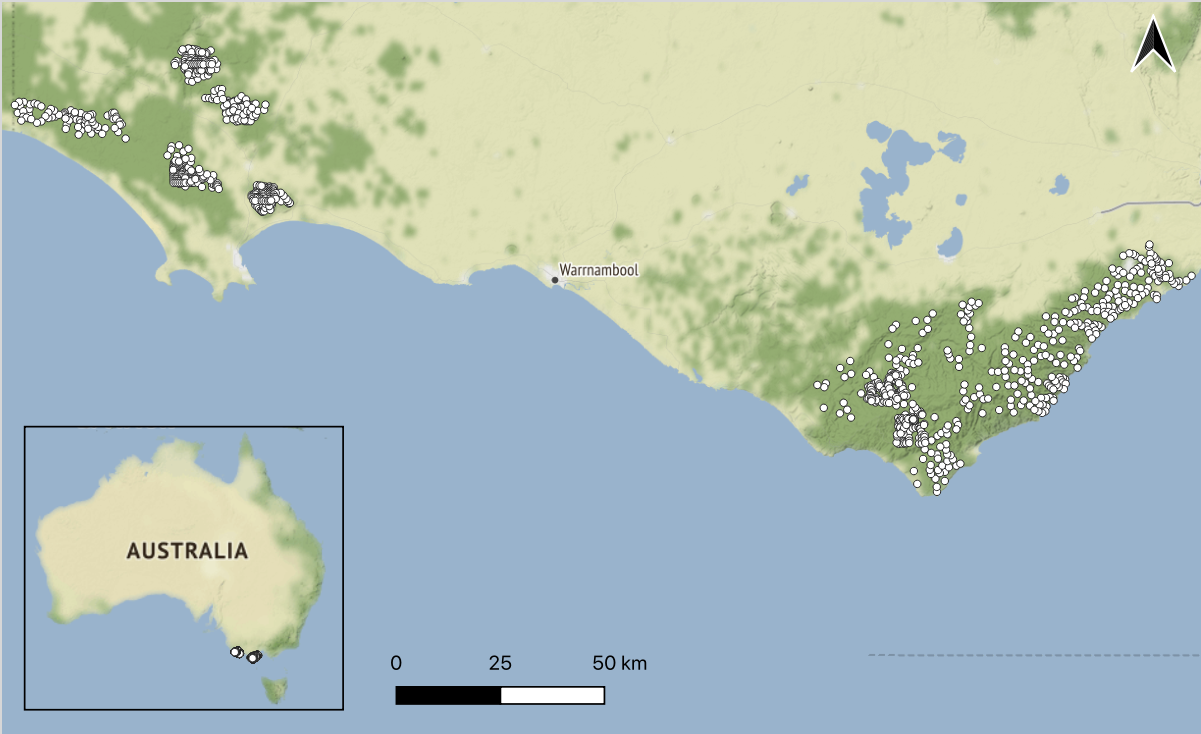
\includegraphics[width=1\linewidth]{figure/map_cams} 

}

\caption{Locations of our study regions in south-west Victoria, Australia. The grids of camera-traps are denoted by white dots. The Glenelg region is to the west and Otway region to the east. Native vegetation is indicated by dark green, with hill shading. \textit{Map tiles by Stamen Design, under CC BY 3.0, map data by OpenStreetMap, under CC BY SA.}}\label{fig:diel-map}
\end{figure}
\newpage

\hypertarget{results-3}{%
\section{Results}\label{results-3}}

Overall, we collated 5,449 and 2,202 independent detections of foxes and cats, respectively (separated by at least 30 minutes) from 172,052 camera-trap nights (Table \ref{tab:diel-tab1}).

\hypertarget{how-does-predator-overall-activity-and-diel-activity-patterns-vary-across-space-model-1-1}{%
\subsection{How does predator overall activity and diel activity patterns vary across space? (model 1)}\label{how-does-predator-overall-activity-and-diel-activity-patterns-vary-across-space-model-1-1}}

Predator activity varied considerably across space and throughout the 24-hour daily cycle, and there was some variation in the predator diel activity patterns across space. On average, both predators showed similar diel activity patterns: mostly nocturnal with peaks in activity around sunrise and sunset (i.e., crepuscular; Fig. \ref{fig:diel-veg}i). The main difference between the species was that fox activity peaked just after sunset and they were less likely to be active during the day than cats. Cats also tended to be more active at sunset relative to sunrise.

Diel activity pattern strength also differed between the species. Fox activity was concentrated strongly at particular times of the day, especially in the Glenelg region where activity varied by up to 371\% throughout the daily cycle (Fig. \ref{fig:diel-space}a). Feral cats had relatively more consistent activity throughout the daily cycle and across regions; the maximum difference in cat activity throughout the daily cycle for any given location was 185\%.

Variation in diel activity patterns across space, as well as differences in overall activity between the predators, was strongest in the Otway Ranges. For example, overall fox activity (Fig. \ref{fig:diel-space-o-fox}) and diel activity pattern strength (Fig. \ref{fig:diel-space}b) were lowest in the south-west Otway Ranges, while feral cat overall activity (Fig. \ref{fig:diel-space-o-cat}) and diel activity pattern strength (Fig. \ref{fig:diel-space}b) were highest in that subregion.

\hypertarget{how-does-predator-overall-activity-and-diel-activity-patterns-vary-across-vegetation-types-model-2-1}{%
\subsection{How does predator overall activity and diel activity patterns vary across vegetation types? (model 2)}\label{how-does-predator-overall-activity-and-diel-activity-patterns-vary-across-vegetation-types-model-2-1}}

Overall levels of fox activity were similar across all vegetation types, except wet forests where fox activity was considerably lower. Overall cat activity was more variable across vegetation types; lowest in heathy woodlands and highest in wet forests (Fig. \ref{fig:diel-veg}b).

Diel activity patterns for foxes were similar across all vegetation type except wet forests; in wet forests, foxes were consistently active throughout the daily cycle (Fig. \ref{fig:diel-veg}a). On the other hand, cats were nocturnal (and most active) in wet forests, but largely crepuscular in all other vegetation types (Fig. \ref{fig:diel-veg}b). For both predators, the random effect for region (Glenelg or Otways) in the vegetation models shrank to near-zero, indicating all variation between the regions was explained by the vegetation covariate and site random intercept.

\hypertarget{do-feral-cats-avoid-foxes-in-space-or-time-model-3-1}{%
\subsection{Do feral cats avoid foxes in space or time? (model 3)}\label{do-feral-cats-avoid-foxes-in-space-or-time-model-3-1}}

Cat spatial activity was relatively unaffected by the fox activity in both habitat types of the Otway Ranges; and, if anything, increased with increasing adjusted fox counts in the Glenelg region (Fig. \ref{fig:diel-cat-fox}), indicating cats did not avoid foxes spatially.

Across all habitat types, feral cat diel activity patterns changed across the gradient of fox activity (Fig. \ref{fig:diel-cat-fox}). In the Glenelg region and Otway dry habitat types, feral cats had a nocturnal-crepuscular diel activity pattern where fox activity was low, but were most active during the day where fox activity was high. In contrast, in the wet forests of the Otway Ranges, feral cats were more strongly nocturnal when fox activity was high.

\newpage
\begin{figure}

{\centering 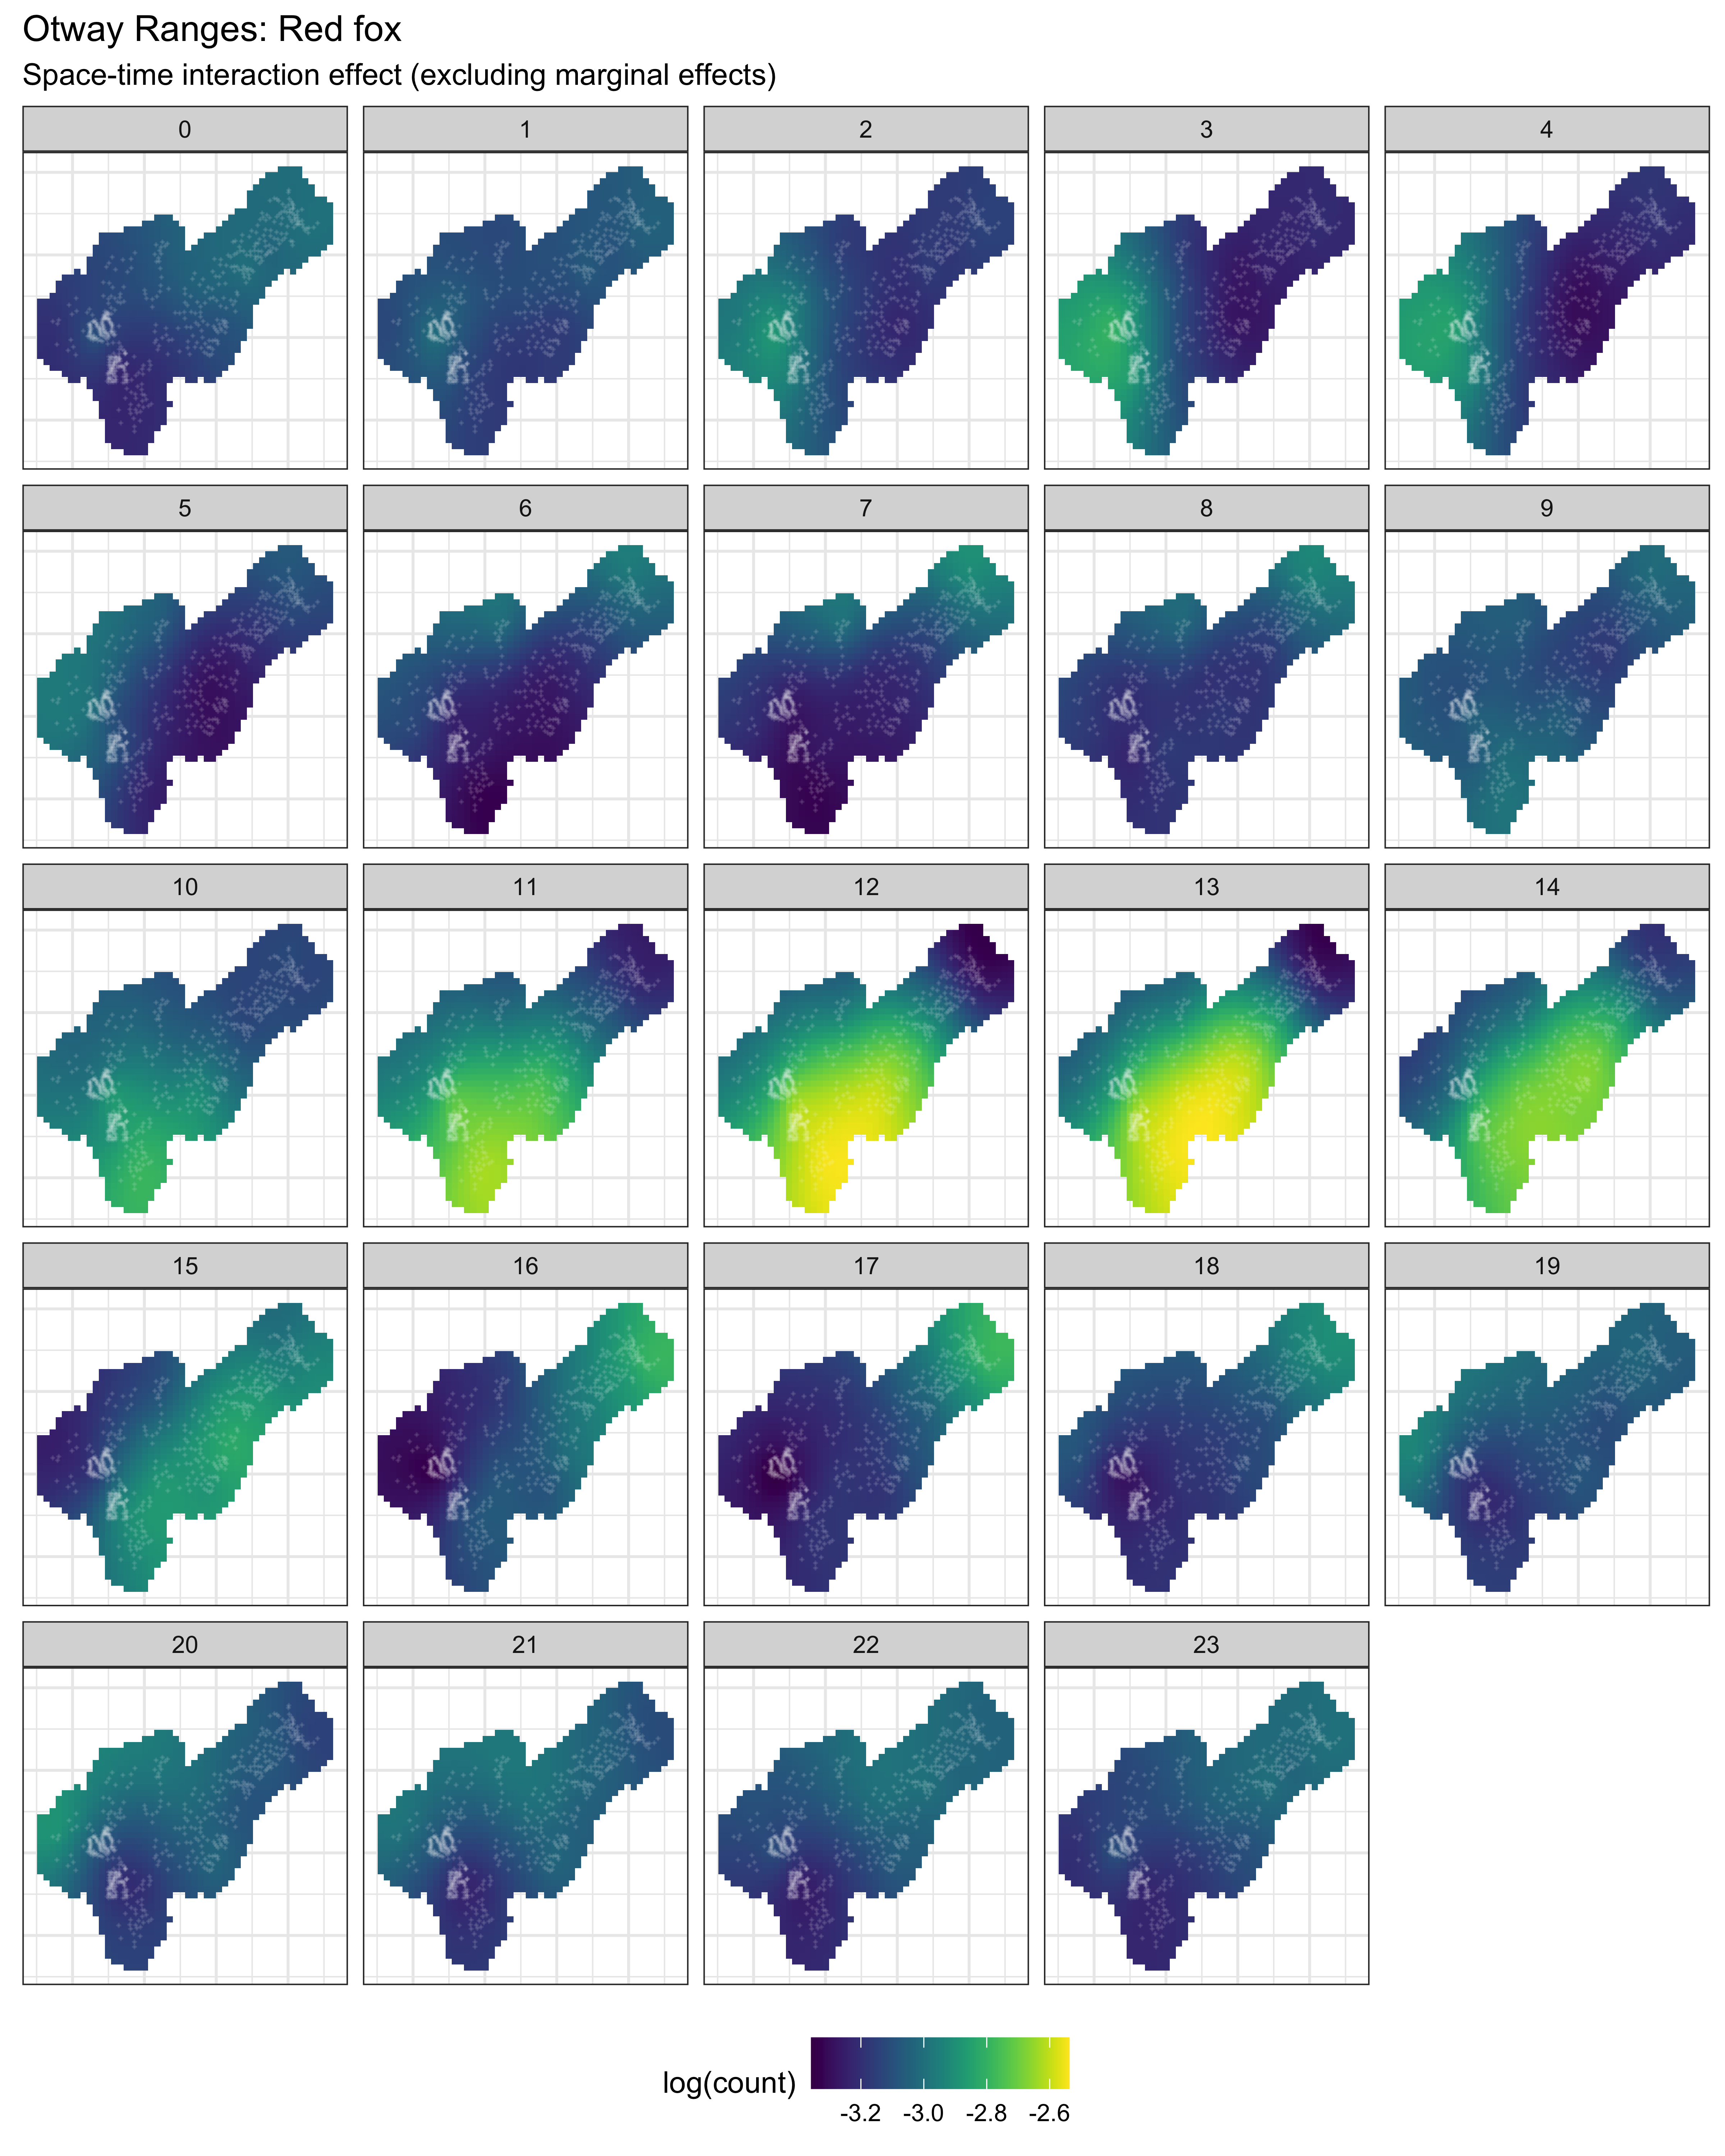
\includegraphics[width=1\linewidth]{figure/spte_diff_avg_o_fox} 

}

\caption{Interaction effect of space-time on red fox \textit{Vulpes vulpes} activity across each hour of the day (0 - 23) in the Otway Ranges, Australia (model 1), as an example. Corresponding plots for the Glenelg region are provided in the Supporting Information, as are the marginal effects of space and time. White crosses depict unique camera-trap sites.}\label{fig:diel-st-int-o-fox}
\end{figure}
\begin{figure}

{\centering 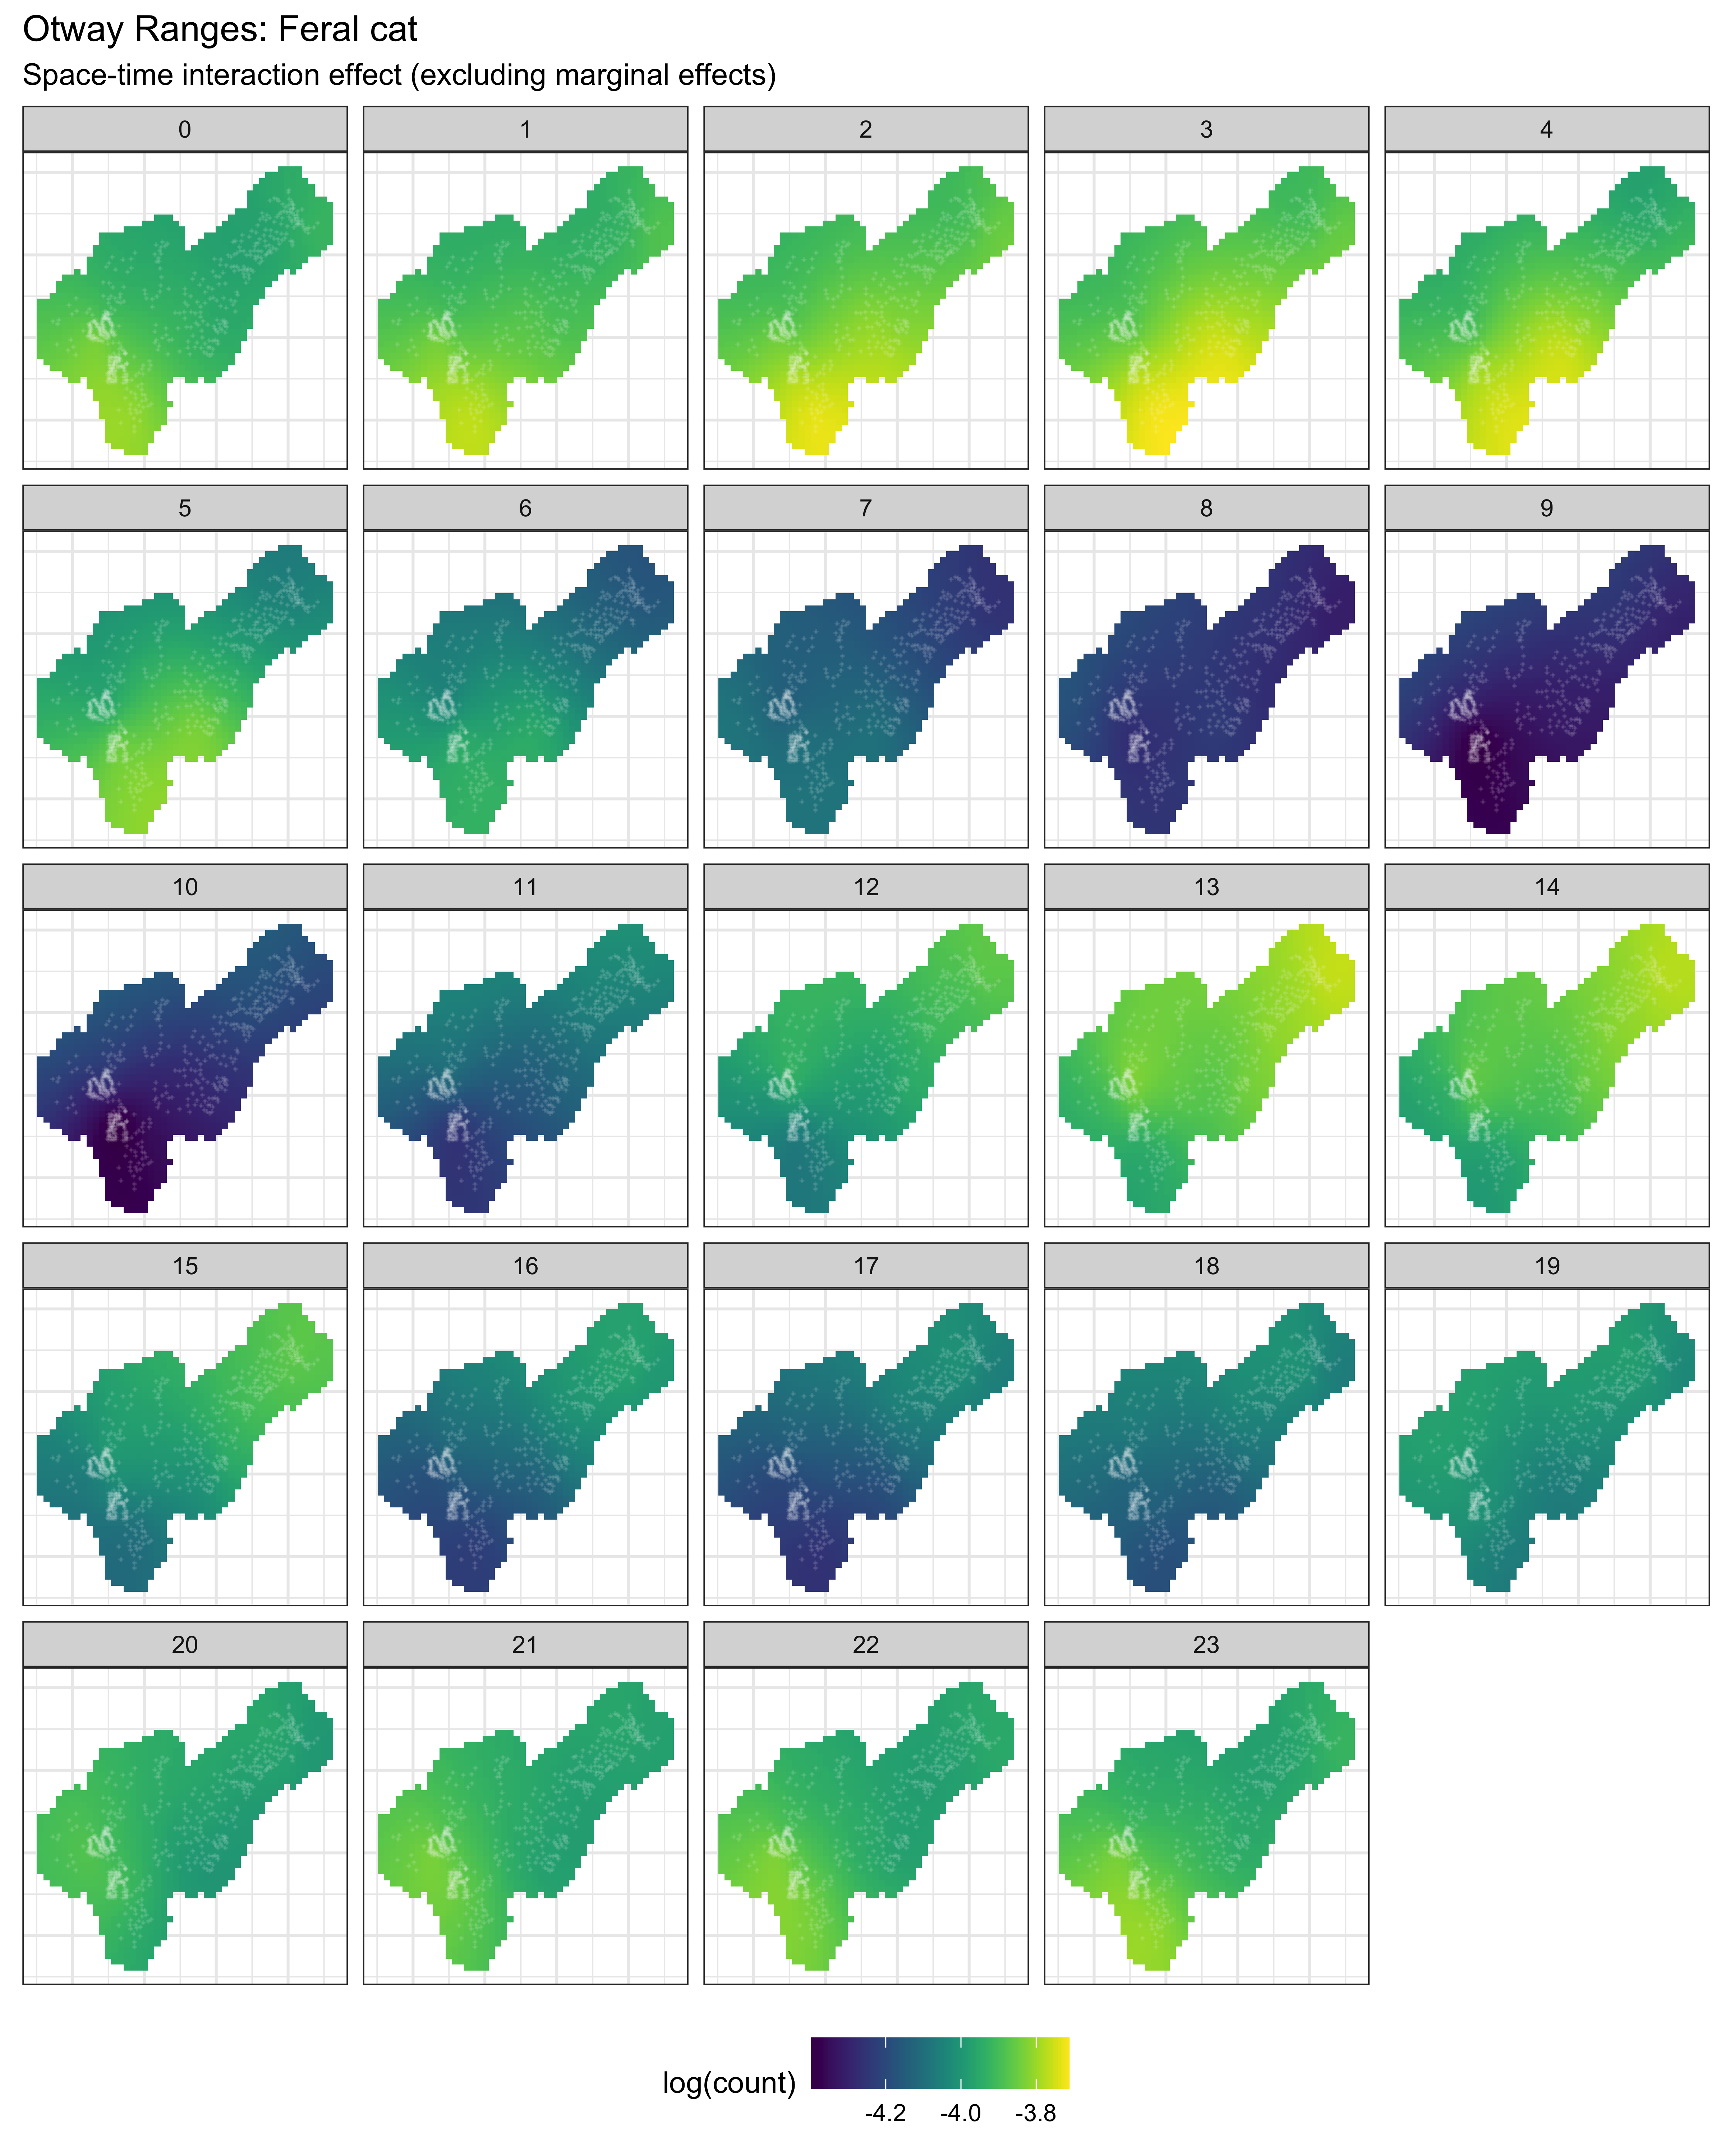
\includegraphics[width=1\linewidth]{figure/spte_diff_avg_o_cat} 

}

\caption{Interaction effect of space-time on feral cat \textit{Felis catus} activity across each hour of the day (0 - 23) in the Otway Ranges, Australia (model 1), as an example. Corresponding plots for the Glenelg region are provided in the Supporting Information, as are the marginal effects of space and time. White crosses depict unique camera-trap sites.}\label{fig:diel-st-int-o-cat}
\end{figure}
\begin{figure}

{\centering 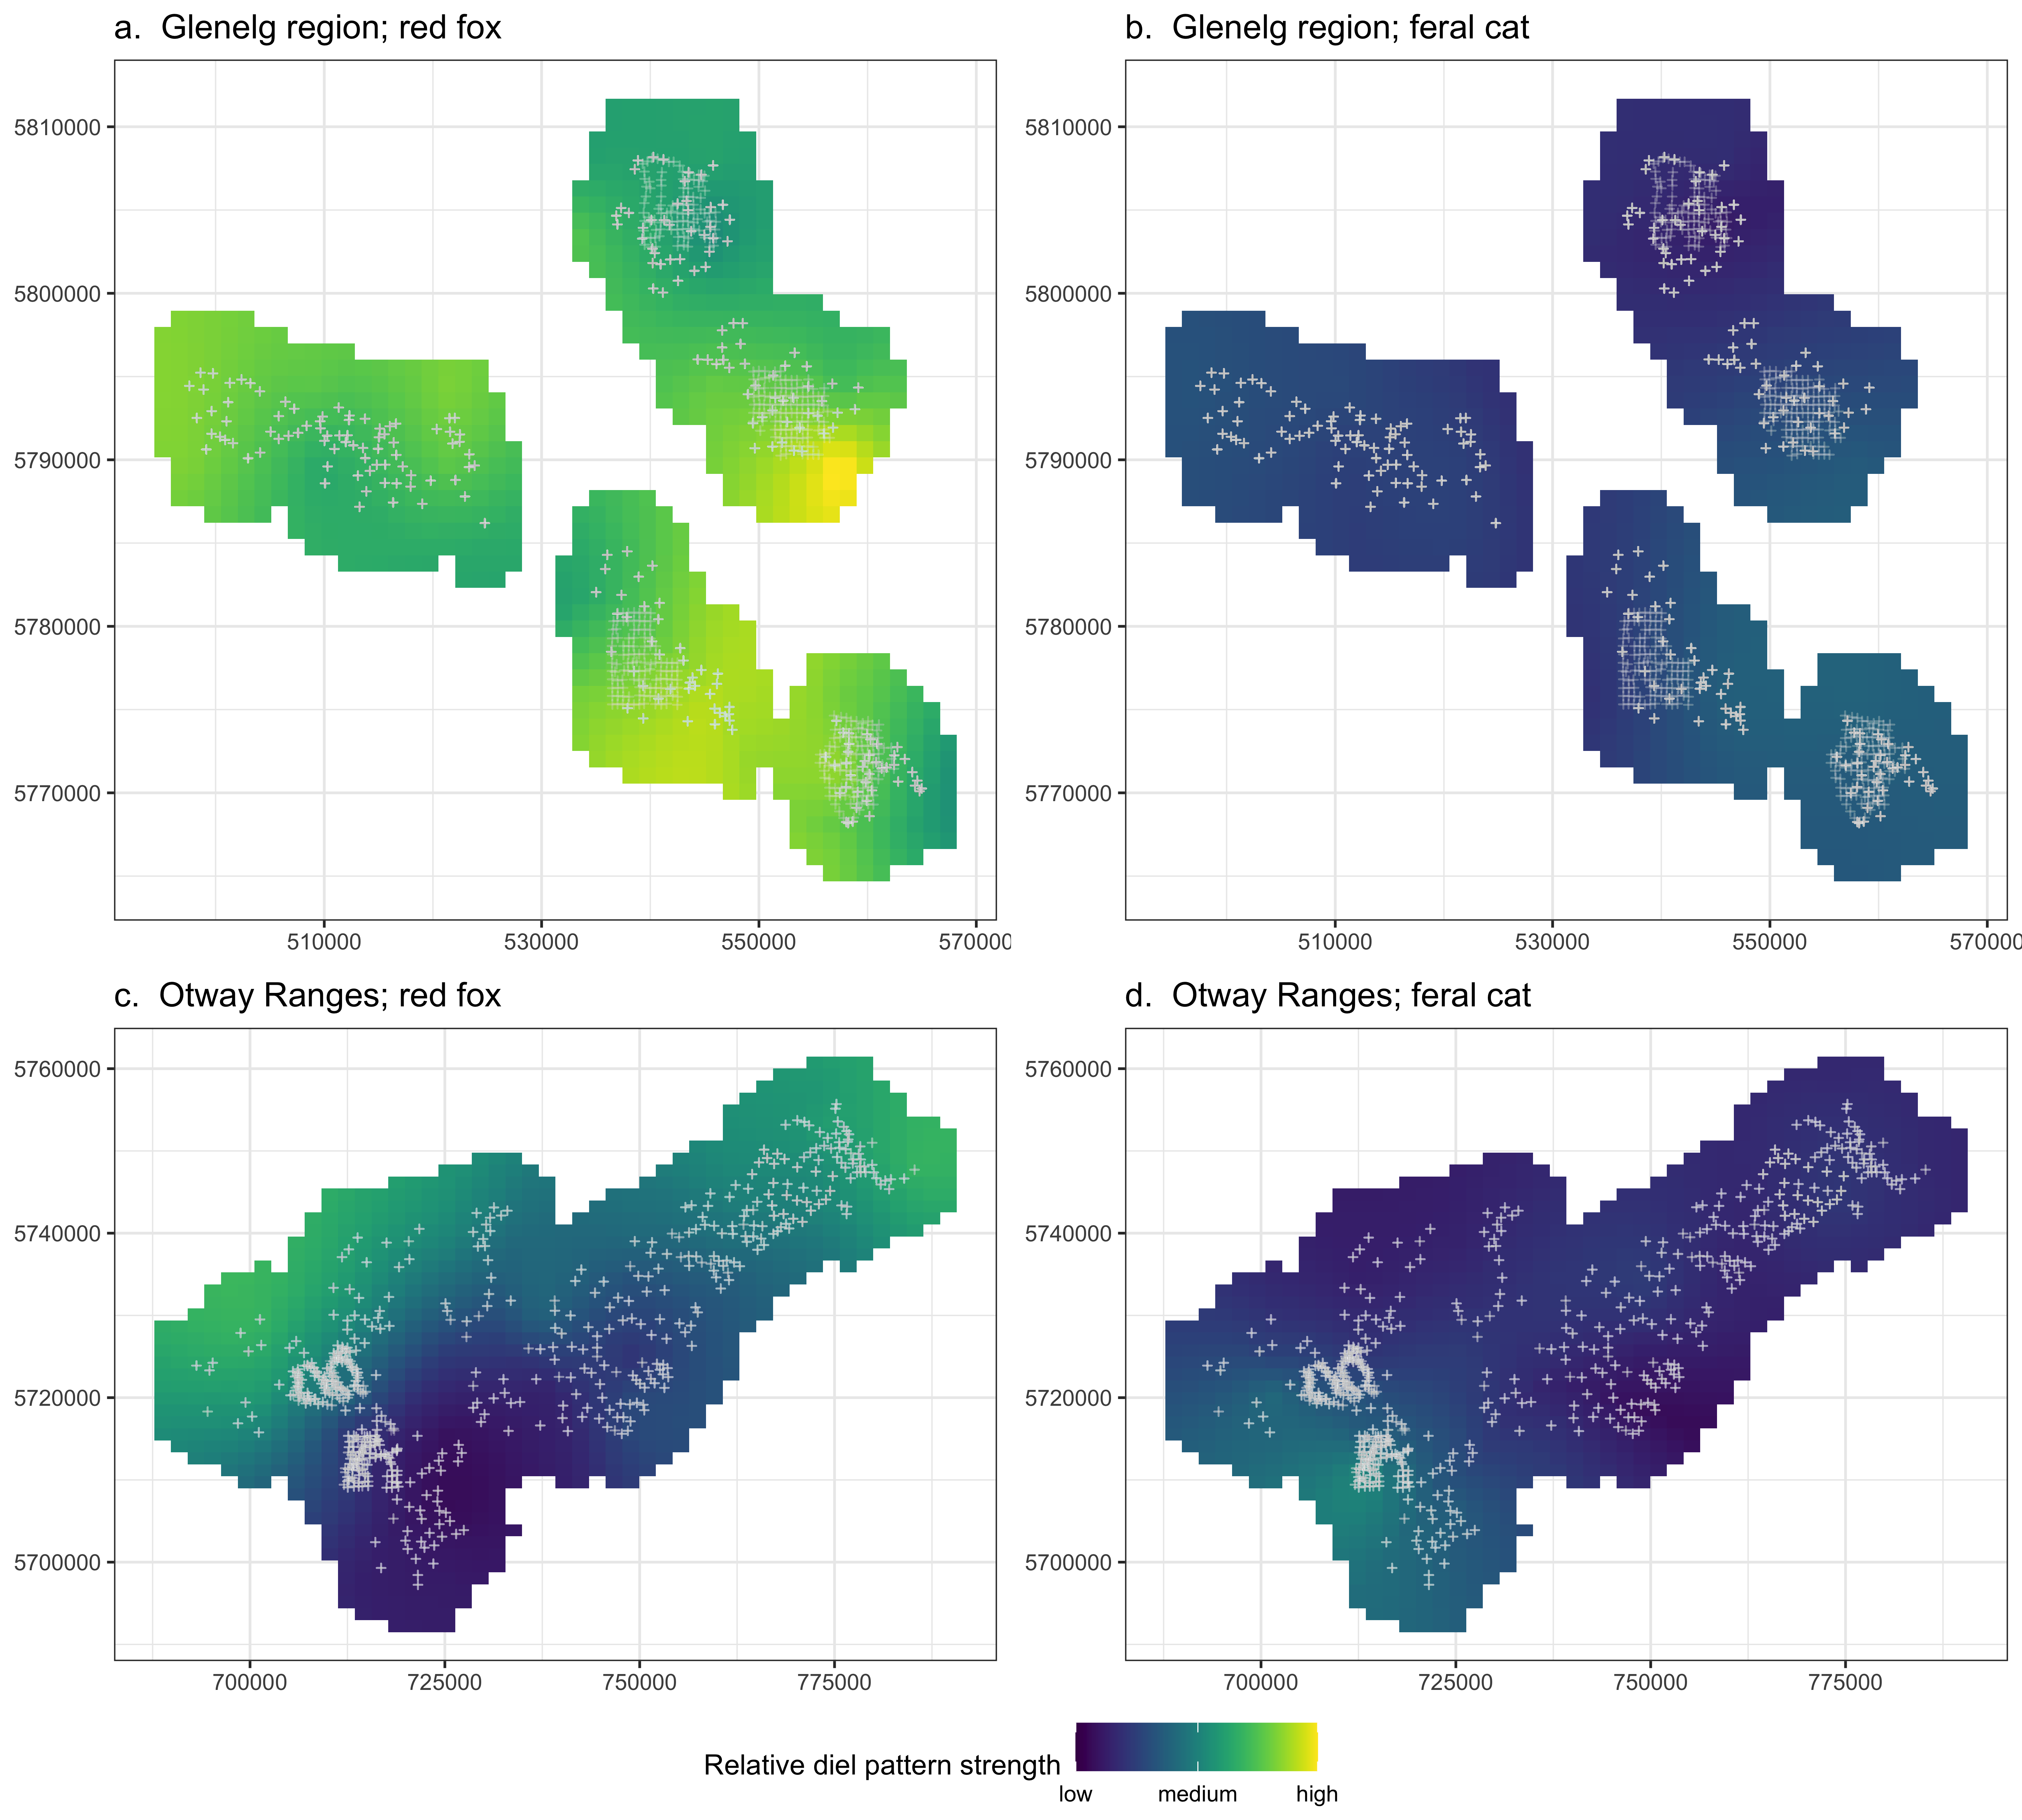
\includegraphics[width=1\linewidth]{figure/diel_strength_600dpi} 

}

\caption{The strength of diel activity patterns of two invasive predators varied within the two study regions in south-west Victoria, Australia (model 1). White crosses depict unique camera-trap sites; colour brightness scales with increasing percentage difference between the minimum and maximum activity estimate over the 24-hour cycle for each location. Red foxes \textit{Vulpes vulpes} (a, c) concentrated their activity during particular times of the day, especially in the Glenelg region (a) and the drier parts of the Otways (c), whereas feral cat \textit{Felis catus} activity was relatively consistent activity throughout the daily cycle (b, d).}\label{fig:diel-space}
\end{figure}
\newpage
\begin{figure}

{\centering 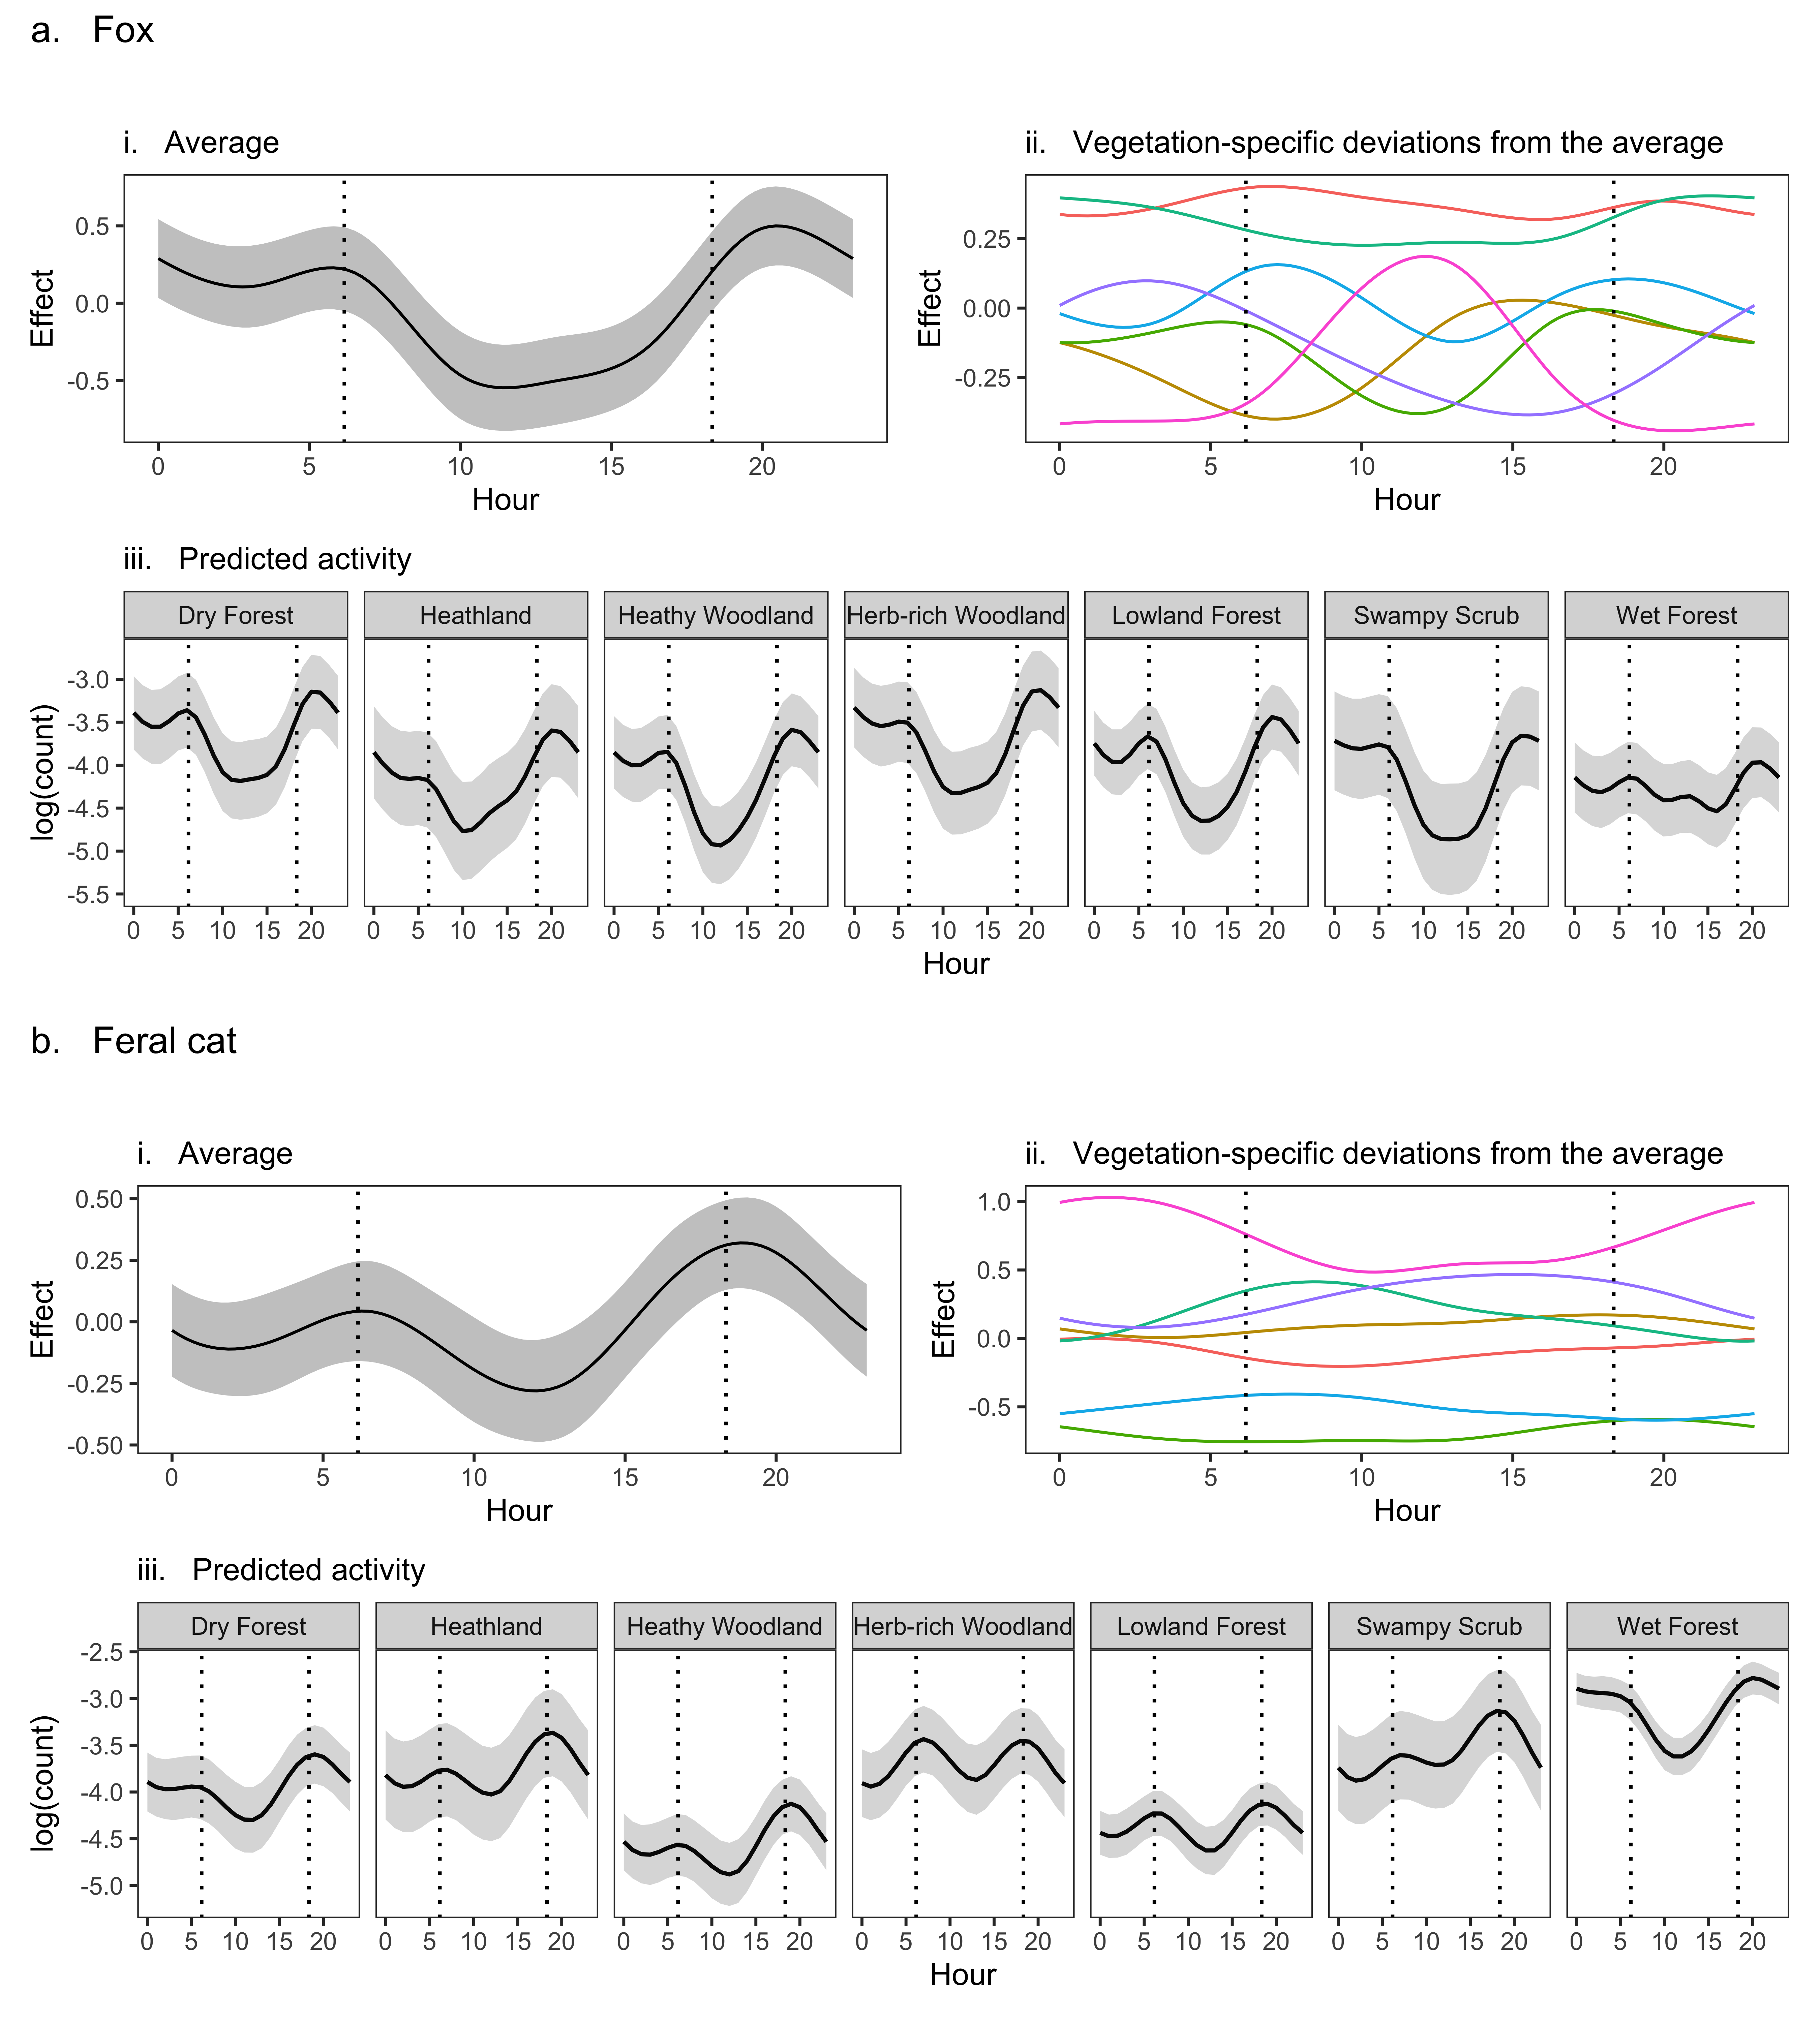
\includegraphics[width=1\linewidth]{figure/predator_veg} 

}

\caption{Red foxes \textit{Vulpes vulpes} (a) and feral cat \textit{Felis catus} (B) diel activity patterns overall (i) and across different Ecological Vegetation Class (EVC) groups (ii, iii) in south-west Victoria, Australia (model 2). Dotted, vertical lines represent average sunrise and sunset times. Shaded areas indicate 95\% confidence intervals. Both invasive predators had a crepuscular to nocturnal diel activity pattern on average, with slight deviations across the drier EVC groups and large deviations in wet forests (ii; wet forests shown as pink line). The overall level of activity was relatively consistent across EVC groups for foxes (a – iii), whereas it differed substantially for feral cats (b - iii).}\label{fig:diel-veg}
\end{figure}
\newpage
\begin{figure}

{\centering 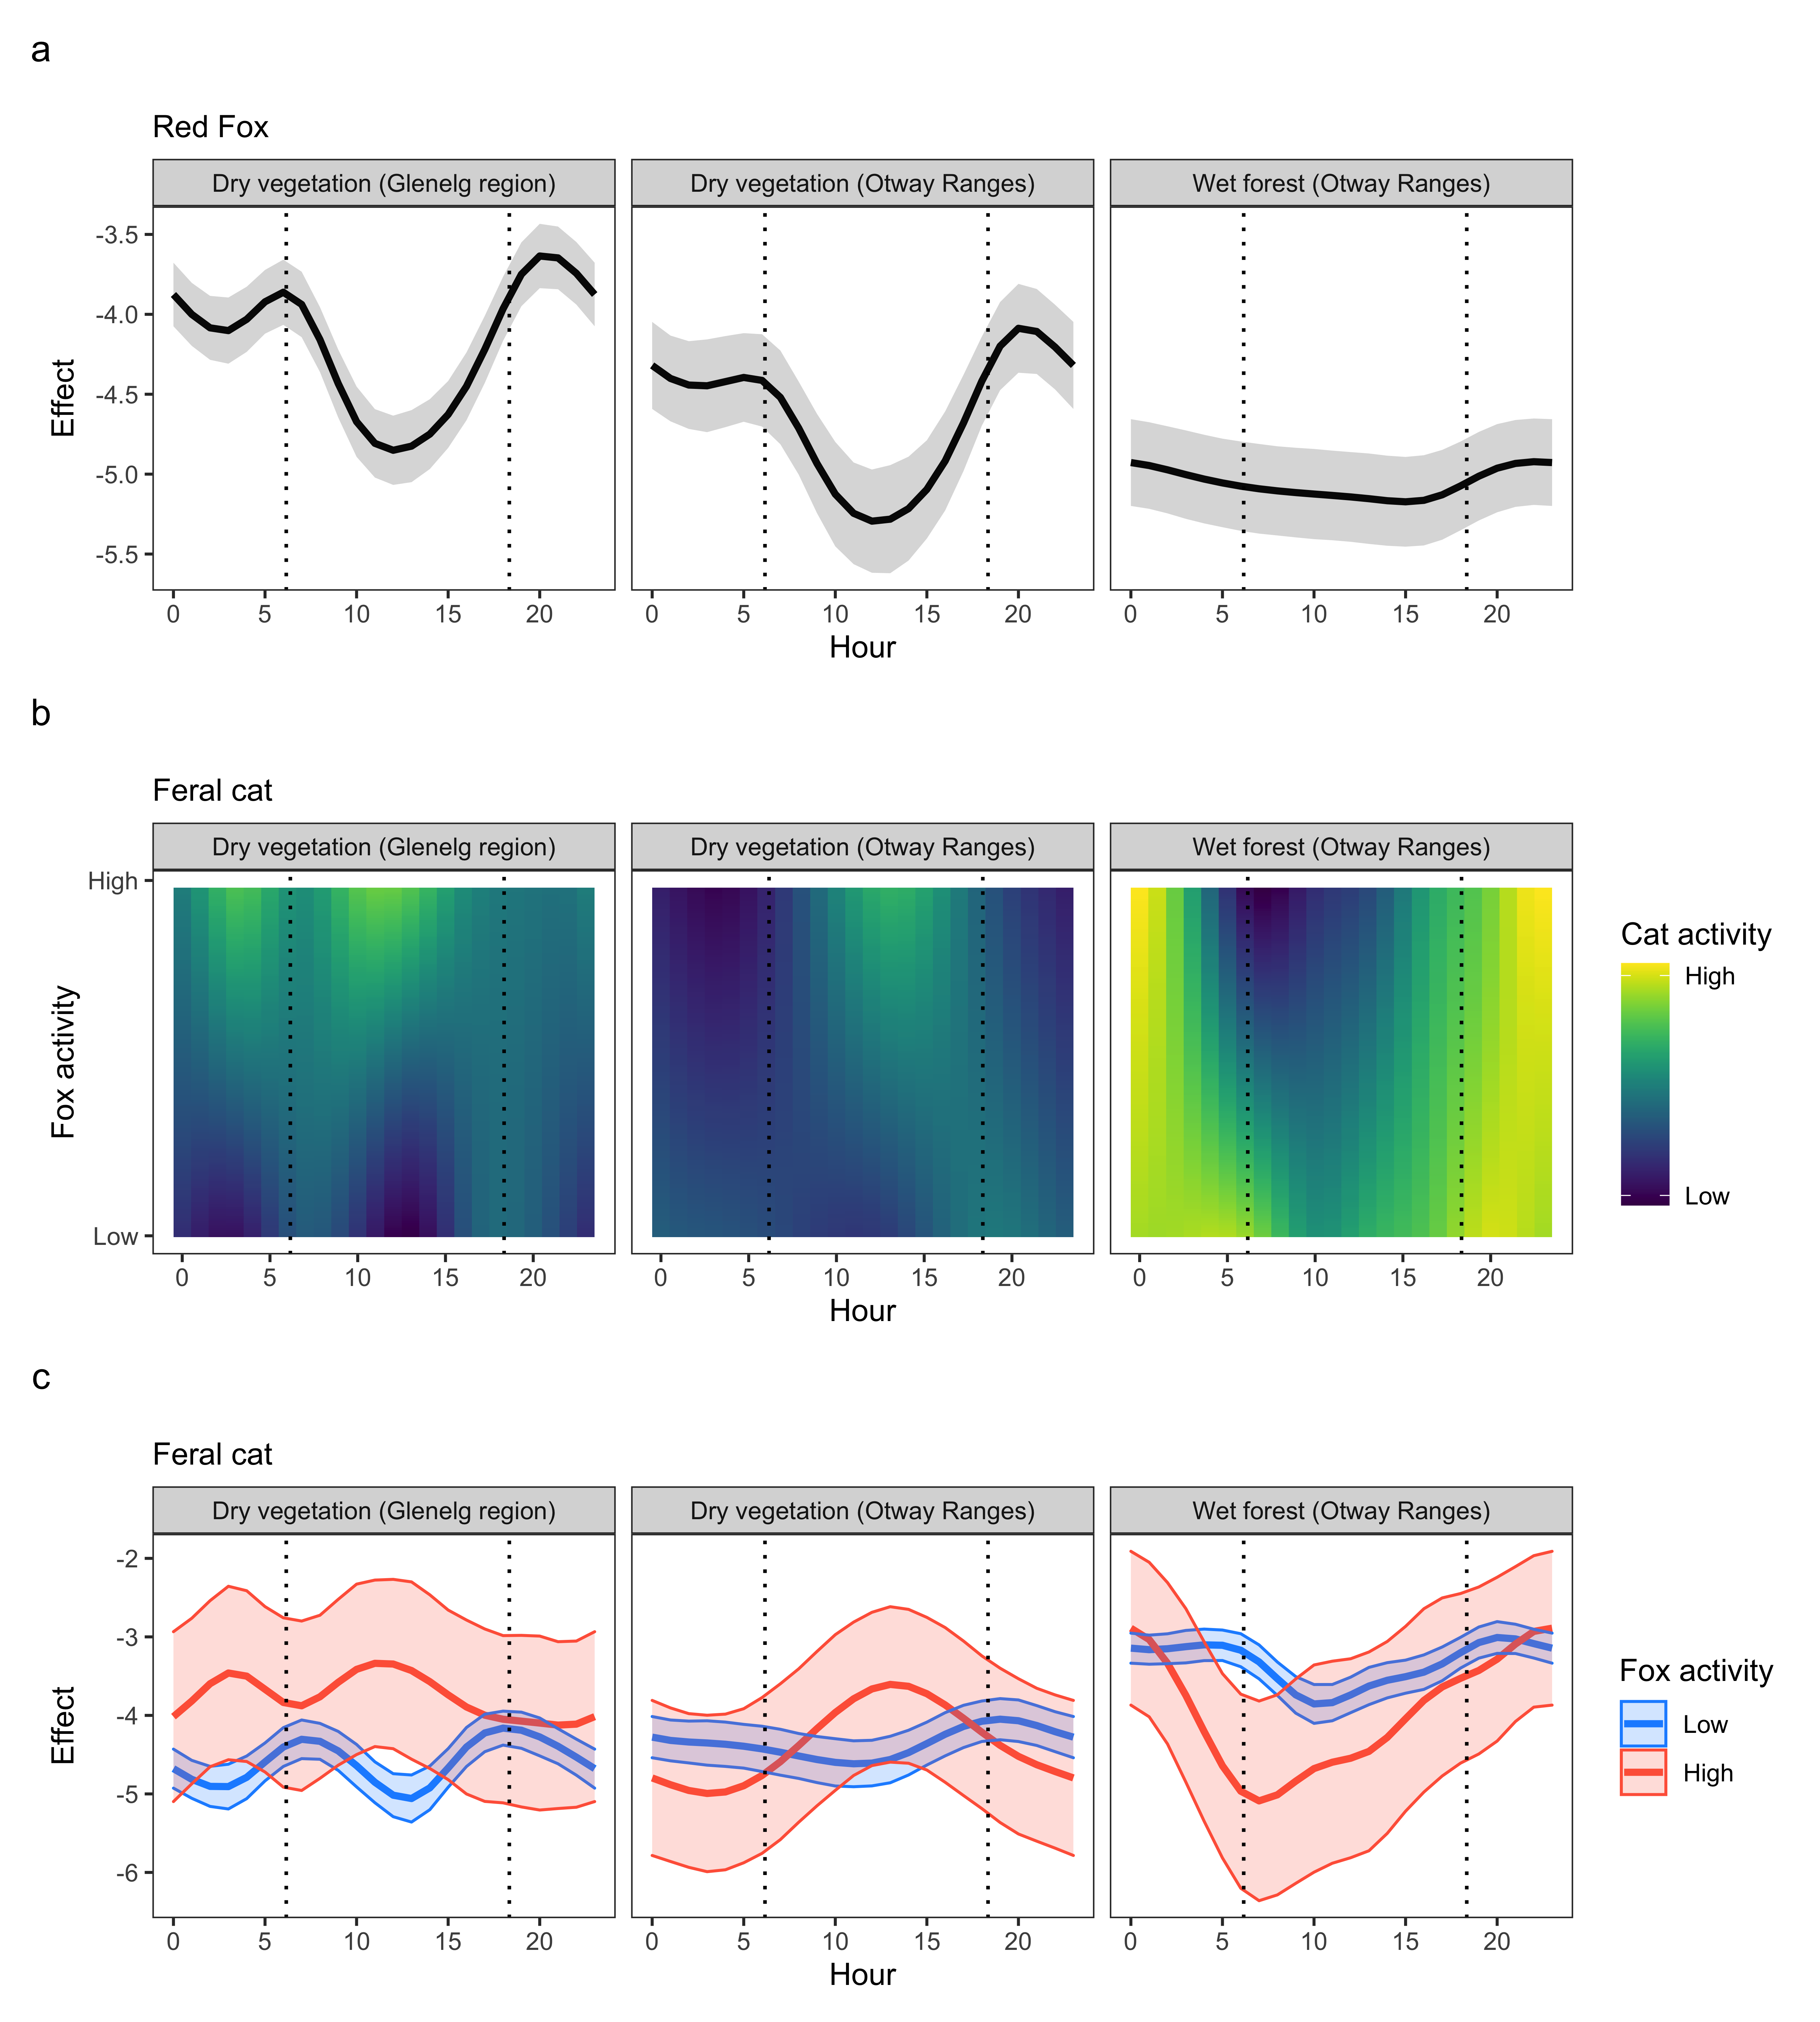
\includegraphics[width=1\linewidth]{figure/cat_fox_count} 

}

\caption{Red fox \textit{Vulpes vulpes} diel activity patterns (a), as well as variation in feral cat \textit{Felis catus} diel activity patterns in response to counts of ’independent’ fox detections (log-transformed and survey effort adjusted) across each habitat type in south-west Victoria, Australia (b; c; model 3). Panels B and C present the same model in two different ways: (b) cat diel activity across the entire continuum of fox activity, (c) cat diel activity patterns at the minimum and maximum fox activity, with associated 95\% confidence intervals (shaded bands). Grey vertical lines represent average sunrise and sunset times. In the Glenelg region, there were more feral cat detections where there were more fox detections, but cat peak diel activity shifted from crepuscular night to pre-dawn and midday (a). In the Otway Ranges, feral cat activity also peaked during the day where fox activity was high in dry vegetation types (b), but was more nocturnal where fox activity was high in the rainforests and wet forests (c).}\label{fig:diel-cat-fox}
\end{figure}
\newpage

\hypertarget{discussion-3}{%
\section{Discussion}\label{discussion-3}}

A key question in ecological theory is whether animals are evolutionary hardwired to occupy particular temporal niches, or have circadian rhythms that are responsive to changing environmental conditions and interactions with other species (Schoener 1974; Daan 1981; Lima \& Dill 1990). Here we demonstrate that diel activity patterns are not fixed, but vary across space based on landscape context and fear. In our study, sympatric invasive predators had similar diel activity patterns when averaged across broad regions (i.e., high circular overlap, Fig. \ref{fig:diel-space-time-marginal}, as did Roshier \& Carter 2021), but behaviours varied considerably within landscapes. Fox daily activity patterns were most strongly tied to the daily cycle in dry habitat types, but showed little diel activity pattern in the wet forests (Fig. \ref{fig:diel-veg}a). In contrast, cats were mostly nocturnal in wet forests but crepuscular in dry vegetation types (Fig. \ref{fig:diel-veg}b). Within broad habitat types, cats altered their diel activity patterns at sites with higher fox activity (Fig. \ref{fig:diel-cat-fox}). Control programs that reduce invasive fox activity are therefore likely to change cat diel activity patterns, which in turn may alter cat impacts on native prey species. Quantifying changes in diel activity patterns provides important context for understanding species interactions, which is key for effective ecosystem management (Gaynor \emph{et al.} 2021).

Shifting diel activity patterns may facilitate spatial coexistence of dominant and subordinate species (Carothers \& Jaksić 1984). For cats, altering diel activity patterns to less-preferred times of day may be worthwhile to persist in high-quality habitat. Few studies have demonstrated predator-induced shifts in diel activity (Kronfeld-Schor \& Dayan 2003), but notably, ship rats \emph{Rattus norvegicus} were also found to switch from nocturnal to diurnal behaviour in response to fox activity (Fenn \& Macdonald 1995) and a similar nocturnal-diurnal shift was observed in American mink \emph{Neovison vison} following the recolonisation of native predators (Harrington \emph{et al.} 2009). For cats in our study, a switch to diurnal behaviour where fox activity was high in the dry vegetation types may have been facilitated by the higher abundance of reptiles in these habitat types relative to wet forests (which are mostly diurnal, Woinarski \emph{et al.} 2018). At wet forest sites with high fox activity, cats concentrated their activity away from sunrise and sunset towards midnight, despite a diurnal shift appearing to similarly reduce the risk of a fox encounter. In this situation, we expect becoming more nocturnal to be favourable over a diurnal shift because this is when small mammals are active and cats would be least visible to foxes (cats here mostly had black or grey coats). Overall fox activity was twice as low in the wet forests relative to dry habitat types, and so cats were likely under less pressure to radically alter their diel activity patterns. Understanding how these potential avoidance behaviours impacts native prey is a key research priority to improve invasive predator management.

Cats may have avoided foxes in time, but we saw no sign of spatial avoidance (i.e.~no fine-scale negative association between fox and cat overall activity (Fig. \ref{fig:diel-cat-fox}b:c). Overlap in spatial activity at fine scales (i.e., at the level of camera-trap sites) may have been facilitated by temporal avoidance (Kronfeld-Schor \& Dayan 2003). However, we considered spatial avoidance across the entire survey duration (averaging 47 days). Cats may indeed avoid foxes spatially, but transiently on the scale of hours to days---after all, how is a cat to know where to avoid a fox without encountering signs of one? Short-term spatial avoidance is quite plausible given foxes mark territories using scats and odours, which cats could tangibly associate with high risk shortly after. Temporary spatial avoidance could be tested using decay curves (e.g., Niedballa \emph{et al.} 2019). Alternatively, no sign of spatial avoidance between these invasive predators could also be an artefact of the quality of camera set-up and hence detectability. The 3,667 camera-traps were deployed by numerous people, and the quality of set-ups differed considerably in terms of detecting predators. Camera-traps that angled only slightly downwards, rather than upwards or strongly downwards, seemed most effective at detecting both predator species (M.W Rees, personal observation). Predator interactions are routinely inferred through spatial associations between species; however such analyses are subject to numerous pitfalls which can make inference unreliable (reviewed in Blanchet, Cazelles, \& Gravel 2020).

A distinction of our study from others is that we modelled potential avoidance behaviours in a simple predator guild, where apex predator activity was artificially manipulated. This reduces potential bias from differences in niche preferences and the unmodelled impacts of other predators in the system. We also included replication across different habitat types. However, because our study did not consider associations with prey species, we cannot distinguish whether changes in cat diel activity patterns were the result of direct fox avoidance or indirect associations with shared prey. For example, low fox activity may promote the availability of a preferred shared prey species with a diel pattern which differs from those of cats on average, and as a result, cats might shift diel activity patterns at sites with low fox activity to more closely match those of the more abundant prey species. We would expect introduced European rabbits \emph{Oryctolagus cuniculus} and hares \emph{Lepus europaeus} (which are diurnal) to be particularly likely to induce such a response in dry vegetation types (McGregor \emph{et al.} 2020; Stobo-Wilson \emph{et al.} 2020a), however, rabbits and hares are rare within the natural vegetation of the landscapes we surveyed (only ever being detected at 40 of 1,232 sites) and there is little evidence that predation by foxes suppresses rabbit populations (Norbury \& Jones 2015; Scroggie \emph{et al.} 2018). While of particular interest, whether temporal fox-cat interactions are direct or indirect does not change the resulting impact on native prey, and hence the outcomes of fox management.

Flexible antipredator behaviours make evolutionary sense, but have been rarely demonstrated in terms of spatiotemporal predator avoidance (although, see Relyea 2003; Brown \emph{et al.} 2013; Cunningham \emph{et al.} 2019), because this often requires manipulative experiments or at least more complicated models (Kronfeld-Schor \& Dayan 2003). Our study demonstrates that GAMs offer a powerful tool for modelling continuous shifts in animal activity across both space and time, capable of capturing complex interactions and sharing information across categorical variables. The inbuilt smoothing penalties are another benefit of GAMs over kernel density estimation (Ridout \& Linkie 2009), in which noisy data can produce spurious estimates (Frey \emph{et al.} 2017; Iannarilli \emph{et al.} 2019). The alternative approach of simply comparing average diel activity overlap between two species (Ridout \& Linkie 2009) would have been misleading for two reasons. Firstly, predator diel activity patterns varied `naturally' across heterogeneous landscapes (requiring avoidance to be tested in wet forests and dry vegetation types separately, Fig. \ref{fig:diel-veg}). Secondly, apex predator temporal avoidance strategies were not consistently employed, but depended on overall apex predator activity and vegetation type (Fig. \ref{fig:diel-cat-fox}). Despite their underlying statistical complexity, GAMs in the `mgcv' R-package are straightforward to fit. Our GAM framework for modelling spatiotemporal activity can be used on any species with time-stamped detections, including datasets with categorical or continuous covariates and hierarchical groupings.

Animal diel activity patterns can be complex, varying across space, habitat types and threat-levels (McCann, Zollner, \& Gilbert 2017). Despite telling an important story about how animals interact with each other and the environment, detection times are commonly discarded from statistical analyses of camera-trap data. In the rare instances that they are considered, diel activity patterns are predominantly estimated at the population-level, overlooking finer-scale behaviours that can affect fitness, survival and ecosystem-impacts. Our results demonstrate the importance of (a) considering diel activity in regards to species interactions, (b) modelling changes in animal behaviour rather than overlap with other species, and (c) testing avoidance behaviours within a joint spatiotemporal framework. Our study adds to the limited body of evidence that top predators can cause fear which is powerful enough to reverse the diel activity patterns of subordinate species (Kronfeld-Schor \& Dayan 2003).

\hypertarget{synthesis}{%
\chapter{Synthesis}\label{synthesis}}

Apex predators can suppress mesopredators and prey through two nonexclusive pathways: density and behavioural mediation (Ripple \emph{et al.} 2016).

In this thesis, I inferred that foxes mediated the density of cats in Chapter \ref{density}. I observed a numerical increase in cats following fox control, and negative associations between fox occurrence probability and cat density at fine spatial scales. More cats in a system following fox control will lead to higher consumption of their prey, although this relationship may not be linear (Abrams 1993; Moseby, Peacock, \& Read 2015) and needs to be weighed against the benefits of having fewer foxes in the system.

Behavioural mediation between an apex and a mesopredator is more difficult to quantify and predict than density mediation (Ford \& Goheen 2015). I found that fox activity likely lowered cat detectability (Chapter \ref{occ}; Chapter \ref{density}) and shifted their diel patterns (Chapter \ref{diel}), potentially reflecting fox avoidance behaviours. A relaxation of cat behaviour following fox control is likely to increase cat hunting success, and/or shift their impacts onto different prey species. However, these patterns were less consistent across my study regions relative to changes in cat density.

In this synthesis, I will examine the evidence for fox control causing a mesopredator release of cats, in terms of both density and behavioural mediation. I will also discuss the potential implications for native prey and hence invasive predator management for conservation, as well as highlight future research priorities throughout.

\hypertarget{density-mediation}{%
\section{Density mediation}\label{density-mediation}}

The classic definition of the mesopredator release hypothesis (hereafter `MRH') is that a decline in the population of an apex predator causes an increase in the density of mesopredators (Soulé \emph{et al.} 1988). Yet, few studies have tested or demonstrated this, partly due to the difficulty of robustly estimating predator density. By using spatially explicit capture-recapture methods which allowed for flexible detection rates, I was able to provide the first evidence that fox control can increase the density of cats (Chapter \ref{density}).

The impact of fox control on cat density---ranging from no effect to a nearly four-fold increase in cat density---appeared dependent on the degree of fox suppression (Chapter \ref{density}). This was further evidenced by a negative relationship between cat density and fox occupancy estimates at fine spatial scales (Fig. \ref{fig:dcor}). The strongest effects came from the Glenelg region (Chapter \ref{density}). Fox control in the Glenelg region has occurred for more than a decade and has substantially reduced fox occupancy rates (Chapter \ref{occ}). Cat density increased with fox control to a smaller extent in the Otway Ranges, which was unsurprising given that (a) fox occurrence in my study area was already low prior to lethal control, (b) fox control only recently commenced, and (c) fox-baits were replaced less frequently than in Glenelg. These results highlight the importance of measuring apex predator activity alongside mesopredator density when testing the MRH, rather than simply relying on binary treatments of apex predator decline (Salo \emph{et al.} 2010; Brook, Johnson, \& Ritchie 2012).

It is hypothesised that apex predators may only place an upper limit on mesopredator density (Johnson \& VanDerWal 2009; Letnic \emph{et al.} 2011). In the Otway Ranges---but not the Glenelg region---the non-linear model supported this hypothesis: cat density was only estimated to decline in the mid-high range of fox occurrence probabilities, while remaining steady at low fox occurrence probabilities (Fig. \ref{fig:dcor}). Further, the nonlinear relationships between fox occurrence probability and cats in the Otway Ranges (Fig. \ref{fig:detcor}; Fig. \ref{fig:dcor}) suggested that a relaxation of cat antipredator behaviours may cause a lagged increase in cat density (Chapter \ref{density}). While speculative, my study is one of the first to be able to test this given my models (a) separated population density from behavioural processes and (b) allowed nonlinear responses.

\hypertarget{behavioural-mediation}{%
\section{Behavioural mediation}\label{behavioural-mediation}}

Recently, the definition of the MRH has been expanded to also capture changes in mesopredator distribution and behaviour following apex predator decline (Brashares \emph{et al.} 2010). In my thesis, I explored these angles using occurrence models (Chapter \ref{occ}), spatial detection rates in cat density models (Chapter \ref{density}), as well as spatiotemporal activity (Chapter \ref{diel}) models. In contrast to the changes in cat density described above, changes in cat behaviour in response to fox activity were relatively inconsistent across replicates and regions. The relationship between the probability of fox occurrence on cat detectability varied between regions. In the Glenelg region, there was little evidence that cat spatial detection rates changed with fox control or across fox occurrence probability gradients (Chapter \ref{density}). In the wet forests of the Otway Ranges, spatial capture-recapture models revealed that cats did not range as far and were more detectable in their activity centre when fox occurrence was low (Fig. \ref{fig:detcor}), suggesting behavioural avoidance. This was supported by occupancy-detection model, which estimated cats to be slightly more detectable with fox control across the Otway Ranges (Fig. \ref{fig:occ-det}a).

Landscape context and the level of perceived risk mediate antipredator strategies (Wirsing \emph{et al.} 2021). A key result of my study is identification of differences in fox and cat ecology between wet and dry vegetation types. Fox occupancy was lowest and cat occurrence was highest in the wet forests relative to dry vegetation types (cat densities were also very high in the wet forests; Chapter \ref{otways17}). Similarly, there were substantial differences in behaviour. Foxes were mostly nocturnal in dry vegetation types but had little variation in activity throughout the daily cycle in wet forests. Cats on the other hand were mostly crepuscular in dry vegetation types, and nocturnal in wet forests. Differences in potential antipredator strategies were further highlighted in Chapter \ref{diel}, which suggested cats avoid foxes temporally by becoming more diurnal in dry vegetation types but by reducing activity around dawn in wet forests (Fig. \ref{fig:diel-cat-fox}). I suspect these difference in antipredator strategies relate to differences in prey species (e.g., diurnal reptiles are scarce in wet forests) and shelter availability (cats likely have more opportunity to escape following a fox encounter in the more structurally complex wet forests), as well as fox encounter rates (lower occurrence probabilities in wet forests) between these habitat types. We have long been aware of the role of predator behavioural mediation in ecosystem function (Schmitz, Beckerman, \& O'Brien 1997), but still have a somewhat poor ability to predict behavioural changes following apex predator decline (Peacor \emph{et al.} 2013; Prugh \emph{et al.} 2019). Testing antipredator responses in mesopredators across a wider range of landscape contexts will be key to further establishing general patterns of behavioural mediation.

There are several other potential ways cats could have altered behaviour following fox control which my thesis did not investigate, such as diet and fine-scale habitat preferences. For example, coupling telemetry and diet analyses, Molsher (1999) found cats increased their use of more open habitat types and consumed more carrion and invertebrates following fox control (Molsher \emph{et al.} 2017). However, following fox eradication on Phillip Island, Rendall \emph{et al.} (2022) found no evidence of prey switching, although cats slightly increased their consumption of invertebrates and black rats \emph{Rattus rattus}. In another forested region of Victoria, Buckmaster (2012) hypothesised that large `holes' in the home range of each GPS-collared cat could be due to apex predator avoidance; in contrast Roshier \& Carter (2021) found no strong evidence that cat distributions were influenced by foxes in an arid region. There is currently no information on cat diet or habitat selection from south-west Victoria, making this a priority for future research to provide a better understanding of both mesopredator release and how cat ecology differs between Australian regions.

\hypertarget{strength-of-evidence-about-mesopredator-release}{%
\section{Strength of evidence about mesopredator release}\label{strength-of-evidence-about-mesopredator-release}}

While my study provides evidence consistent with the MRH, it had several limitations. In the Glenelg region, I cannot be sure that feral cat density or occupancy did not differ between impact than non-impact landscapes prior to fox control commencing (because there is no available data). However, the spatial replication of the control-impact experimental design (three paired impact and non-impact landscapes) increases confidence in the accuracy of my results. I was able to overcome this limitation in the western Otway Ranges by using a Before-After-Control-Impact-Paired-Series (BACIPS) design. However, effects of fox control were weaker in the Otway Ranges relative to the Glenelg region and there was some overlapping of confidence intervals, indicating weak statistical evidence for mesopredator release. Further, I was unable to replicate the BACIPS design in the Otway Ranges, increasing the vulnerability to type I error (i.e., falsely inferring there was an effect of fox control on cats, Conquest 2000). These issues are common limitations with predator management experiments (Ford \& Goheen 2015) but can still provide robust, clear evidence when ultimately combined in meta-analyses.

A key source of contention around the MRH is the use of associative rather than causal inference (e.g., Allen \emph{et al.} 2013; Hayward \emph{et al.} 2015). Replicated experimental treatments (e.g., fox control and no fox control) are often considered the `gold standard' in experimental designs. However, experimental treatments are often imperfect in large scale ecological field experiments because treatment effectiveness varies (Ford \& Goheen 2015; among several other reasons, Kimmel \emph{et al.} 2021). An increasingly valued alternative to replicated experiment treatments is testing responses across experimental gradients (Ford \& Goheen 2015). Testing responses across experimental gradients (e.g., fox occurrence when subject to lethal control) strengthens inference relative to `natural' observation data and is more feasible to implement relative to replicated large-scale predator treatments (Ford \& Goheen 2015). Experimental gradients are particularly important when responses are nonlinear (Kreyling \emph{et al.} 2018), as intraguild predator interactions are often thought to be (e.g., Letnic \emph{et al.} 2011).

My thesis is unique in that I combined traditional experimental treatment designs and experimental gradients (with both linear and nonlinear regression methods) to test the MRH with the same datasets. Both approaches provided causal inference because foxes were artificially manipulated, and fox control was not knowingly confounded with other variables (except latitude in the Glenelg region - all treatment landscapes were slightly south of the non-treatment landscapes). The addition of experimental gradients was particularly useful in the Otway Ranges where fox control effort was inconsistent; simplifying fox control into a binary treatment variable overlooked important nuance such as bait density and replacement schedules. Quantifying fox activity along gradients expressly measured the likelihood of cats encountering foxes and so provided a more accurate reflection of intraguild predator interactions. Traditional experimental designs are often called for in testing the MRH (e.g., Glen \emph{et al.} 2007; Hayward \emph{et al.} 2015), but a range of experimental approaches can provide complementary and robust causative inference on management interventions (Ford \& Goheen 2015).

Given the consistency and long-term nature of fox control in the Glenelg region, it is likely that predator-predator and predator-prey interactions have stabilised since fox control commenced (i.e., the effect of fox control has had a chance to distil and be detected). This is unlikely to be the case in the Otway Ranges, given we only monitored for 1.5 years following the commencement of fox control and during this time, the control effort was inconsistent. This makes it difficult to draw long-term conclusions around species interactions in the Otways from our observations (Yodzis 1988). I recommend these surveys be repeated in the longer term to provide a better understanding of the impact of fox control. Longer-term surveys in the western Otway Ranges would be provide rich information on fox-cat-prey interactions given the relative absence of other disturbances compared to other regions in Australia which likely have more transient dynamics (e.g., Greenville \emph{et al.} 2014).

Two major constraints to the widespread use of spatial capture-recapture surveys to monitor cat populations are (i) the long and arduous process of individual cat identification and (ii) obtaining sufficient statistical power to detect population changes in a before-after-control-impact design (Efford \& Boulanger 2019). To address one of the most time-consuming parts of the survey process, collaborators and I have been trialling machine learning methods to automatically identify species and individual cats from camera-trap images; these show promise and are likely to increase the feasibility of such studies by management agencies (Yang \emph{et al.} 2021). Nonetheless, reliable estimates from spatial mark-resight models require large sample sizes, which were difficult to obtain, despite extensive and intensive survey effort (41,216 trap nights) and the Otway study region having one of the highest density populations of cats on the Australian mainland (Chapter \ref{otways17}). For regions with lower densities of cats, sufficient sample sizes may be more feasibly achieved using clustered spacing of camera-traps over larger areas rather than the grid designs we used (Sun, Fuller, \& Royle 2014; Clark 2019). A key benefit of spatial capture-recapture studies is that differences in study designs can be accounted for analytically, allowing feral cat density estimates to be collated across different landscapes, regions and fox control programs. This will be particularly important to identify how different management regimes and landscape contexts impact the strength and occurrence of mesopredator release.

\hypertarget{direct-or-indirect-suppression}{%
\section{Direct or indirect suppression?}\label{direct-or-indirect-suppression}}

Mesopredator release following the decline of an apex predator population can occur directly due to a decrease in aggressive encounters experienced by the mesopredator, or indirectly through increased availability of shared prey (Prugh \emph{et al.} 2009). These pathways are difficult to tease apart in my study system, given I studied similar sized predator species in a depauperate predator guild, and so both direct and indirect effects are expected to be strong (Donadio \& Buskirk 2006; Brashares \emph{et al.} 2010; Prugh \& Sivy 2020). The negative correlations between fine-scale cat density and fox occurrence I observed (Chapter \ref{density}) supports a direct top-down suppressive effects of foxes on cats. Ascertaining the contribution of indirect prey effects in mesopredator release would require a negative association between foxes and prey, but it is unclear whether a positive or negative association with cats and prey signal competitor release: a positive association could infer cats are tracking the prey or alternatively, be interpreted as peaceful coexistence.

Prey abundance often increases dramatically several years after fox control (Duncan \emph{et al.} 2020), which could explain why cat activity also tends to increase (Hunter \emph{et al.} 2018), and prey populations often subsequently crash (Duncan \emph{et al.} 2020). Duncan \emph{et al.} (2020) hypothesised that these trends were due to prey overshooting carrying capacity following the release from top-down suppression by foxes; however, our study offers an additional explanation by demonstrating that cat density steadily increases following the commencement of fox control (Otway Ranges) and may remain relatively high in the long-term (Glenelg region). There is currently very little information on how prey availability impacts cat density, particularly in temperate regions (Legge \emph{et al.} 2017), which makes it difficult to understand the relative importance of direct and indirect mesopredator release effects. Nonetheless, this information may not actually be relevant to decision-making around predator management---if fox control increases cat impacts on native prey, does it matter what mechanisms are responsible?

\hypertarget{piecing-together-mesopredator-release}{%
\section{Piecing together mesopredator release}\label{piecing-together-mesopredator-release}}

My thesis provides evidence that fox control frees cats from top-down constraints on population density and diel activity patterns in temperate forests, meeting the definitions of mesopredator release (Prugh \emph{et al.} 2009; Brashares \emph{et al.} 2010; Jachowski \emph{et al.} 2020). A key strength of my thesis is that I investigated interactions between these two species in simplified predator guilds, and from several different angles, with replication across two distinct study regions.

Cats are ubiquitous across Australia (Legge \emph{et al.} 2017) and my study regions. My study concurs with numerous others which have shown little-no evidence that apex predators restrict the spatial distribution of cats {[}e.g., Edwards \emph{et al.} (2002); Brook, Johnson, \& Ritchie (2012); Wang \& Fisher (2012); Fancourt \emph{et al.} (2019); Stobo-Wilson \emph{et al.} (2020b); Roshier \& Carter (2021);{]}; however, I found that cats changed their behaviour and had lower population densities where foxes were common. Spatial co-occurrence between predator species is increasingly used to test the MRH (Jachowski \emph{et al.} 2020), but can be a poor proxy for species interactions (Blanchet, Cazelles, \& Gravel 2020) and overlook other antipredator behaviours, such as reactive spatial avoidance (Broekhuis \emph{et al.} 2013), and temporal avoidance (Kronfeld-Schor \& Dayan 2003). The use of different analytical methods and population metrics helped identify that mesopredator release manifests in different ways, which may have important consequences for biodiversity conservation (discussed in the section below).

While there are several limitations of this study, I believe it provides an important case study for the MRH. High-profile examples of mesopredator release are largely based on the complete extirpation of apex predators---rather than population suppression---often without replication (e.g., Rayner \emph{et al.} 2007). This has led to uncertainty around the generalisability of mesopredator release and whether lethal predator control programs are sufficient to trigger mesopredator release (Ford \& Goheen 2015). My study increases confidence that mesopredator release can occur predictably across different regions (at least in terms of population density), although the strength of the effects depends on the degree of apex predator suppression.

\hypertarget{implications-of-mesopredator-release-for-native-prey}{%
\section{Implications of mesopredator release for native prey}\label{implications-of-mesopredator-release-for-native-prey}}

The primary aim of this thesis was to understand whether mesopredator release was occurring rather than its implications for native fauna. Nonetheless, I found that long-nosed potoroos strongly benefit from fox control in terms of site occurrence in the Glenelg region regardless of any mesopredator release of cats (but not the Otway Ranges). In contrast, southern brown bandicoots showed no response to fox control in terms of occurrence, potentially because they are more susceptible to cat predation.

It is likely that fox control will benefit some native prey, but not others. There is high dietary overlap between foxes and cats; however some native prey, particularly larger species, are more susceptible to foxes than cats (Stobo-Wilson \emph{et al.} 2021b; Stobo-Wilson \emph{et al.} 2021a; Woinarski \emph{et al.} 2021). For example, a density of 0.03 foxes km\textsuperscript{-2} drove a reintroduced population of burrowing bettongs \emph{Bettongia lesueur} to extinction within 12 months in the absence of cats, but another population persisted with no foxes and up to 0.46 cats km\textsuperscript{-2} (Moseby \emph{et al.} 2019). While there is currently no statistical evidence that the size of native prey affects their response to fox control (Hunter \emph{et al.} 2018), the prey species expected to benefit the most from fox control, in particular macropods, are often the focus of associated monitoring programs. More work is needed to examine the responses of different prey species to fox control, particularly smaller species (e.g.~rodents and small dasyurids), which are more sensitive to cat predation.

If fox control increases the density of feral cats, it is likely that the impact of feral cats on native fauna will increase. However, it is important to note that predation rates of particular species may not necessarily increase linearly with cat population density. Predation rates depends on cat demographics (Moseby, Peacock, \& Read 2015), individual specialisation (Dickman \& Newsome 2015), as well as predator and prey behaviour (Abrams 1993) and microhabitat context (McGregor \emph{et al.} 2015a). In some cases, a small number of cats can inflict large damage to local fauna populations (Greenwell, Calver, \& Loneragan 2019; Moseby \emph{et al.} 2019; Tuft \emph{et al.} 2021).

There is concern that large macropods (kangaroos and wallabies) may become overabundant following fox control (as foxes are their primary terrestrial predators where dingoes are absent), thereby increasing their grazing pressure (Doherty \& Ritchie 2017). In turn, this could reduce the understorey habitat structure required by smaller prey species for shelter, and consequently increase prey exposure to invasive predators. There is some evidence to support this (Banks, Newsome, \& Dickman 2000; Dexter \emph{et al.} 2013). Geary \emph{et al.} (2020) found no effect of fox control on herbivore occurrence in the Glenelg region, but herbivore release in terms of density, recruitment rates and behaviour are worth further investigation.

Changes in cat diel activity patterns following fox control could cause cats to switch prey species. Cats are mostly nocturnal, partly because they are likely tracking the activity of small mammals, their preferred prey species (Doherty \emph{et al.} 2015a). I found that cats in dry vegetation types shifted to predominantly diurnal behaviour where fox activity was high (Fig. \ref{fig:diel-cat-fox}). I expect this to shift impacts from small mammals to mostly reptiles and birds which are active during the day. However, in wet forests, cats reduced activity at dawn in response to high fox activity (Fig. \ref{fig:diel-cat-fox}), limiting the total amount of time spent hunting. Further, cats were less detectable in their activity centres in wet forests, potentially reflecting a more cautious hunting strategy (Chapter \ref{density}). It is therefore plausible that fox suppression may increase the impact of cats on native prey, although perhaps onto different species. Given our current lack of ability to generalise behaviour changes and understanding about how different predator behaviours impact prey, this is a strong priority for future research (Wirsing \emph{et al.} 2021).

These factors make it difficult to predict what impact mesopredator release of feral cats will have on native prey of concern. Even with mesopredator release of feral cats, fox control has value as a conservation action (Hunter \emph{et al.} 2018). However, fox control programs are rarely monitored in ways which can reliably detect which species are responding positively, neutrally or negatively to fox control (Reddiex \& Forsyth 2006; Reddiex \emph{et al.} 2007). I hope my thesis does not discourage the use of targeted fox control but encourages the careful monitoring of feral cats and a wider range of shared prey taxa (particularly species that might be highly vulnerable to cats). If cat density increases considerably, or particular native species show signs of decline, lethal cat control should be integrated with fox control (e.g., Comer \emph{et al.} 2020). We must recognise, however, that integrated predator control can be challenging, particularly in temperate environments where broadscale cat control is largely infeasible (Fisher \emph{et al.} 2015; Lazenby, Mooney, \& Dickman 2015). Indirect predator management, such as invasive prey (McGregor \emph{et al.} 2020) or large herbivore (Stobo-Wilson \emph{et al.} 2020b) management, or more targeted prey species-specific conservation actions could also be employed. In dire situations, fox control could be ceased, however this would lose the earlier value of fox control. The singular control of an invasive predator may take the pressure off some native species, but is unlikely to improve the persistence of all native prey species in systems where multiple invasive predators co-occur.

\hypertarget{references}{%
\chapter*{References}\label{references}}
\addcontentsline{toc}{chapter}{References}

\markboth{References}{References}

\noindent

\setlength{\parindent}{-0.20in}
\setlength{\leftskip}{0.20in}

\hypertarget{refs}{}
\begin{CSLReferences}{1}{0}
\leavevmode\vadjust pre{\hypertarget{ref-abbott2008spread}{}}%
Abbott, I. (2008) \href{https://www.dpaw.wa.gov.au/images/documents/about/science/cswa/articles/23.pdf}{The spread of the cat, \emph{{F}elis catus}, in {A}ustralia: Re-examination of the current conceptual model with additional information.} \emph{Conservation Science Western {A}ustralia}, \textbf{7}.

\leavevmode\vadjust pre{\hypertarget{ref-abrams1993predation}{}}%
Abrams, P.A. (1993) \href{https://doi.org/10.2307/1940800}{Why predation rate should not be proportional to predator density}. \emph{Ecology}, \textbf{74}, 726--733.

\leavevmode\vadjust pre{\hypertarget{ref-algar2020feral}{}}%
Algar, D., Johnston, M., Tiller, C., Onus, M., Fletcher, J., Desmond, G., Hamilton, N. \& Speldewinde, P. (2020) \href{https://doi.org/10.1007/s10530-019-02154-y}{Feral cat eradication on {Dirk Hartog Island, Western {A}ustralia}}. \emph{Biological Invasions}, \textbf{22}, 1037--1054.

\leavevmode\vadjust pre{\hypertarget{ref-allen2017can}{}}%
Allen, B.L., Allen, L.R., Andrén, H., Ballard, G., Boitani, L., Engeman, R.M., Fleming, P.J., Ford, A.T., Haswell, P.M., Kowalczyk, R. \& others. (2017) \href{https://doi.org/10.1016/j.fooweb.2017.02.008}{Can we save large carnivores without losing large carnivore science?} \emph{Food Webs}, \textbf{12}, 64--75.

\leavevmode\vadjust pre{\hypertarget{ref-allen2022fear}{}}%
Allen, M.C., Clinchy, M. \& Zanette, L.Y. (2022) \href{https://doi.org/10.1073/pnas.2112404119}{Fear of predators in free-living wildlife reduces population growth over generations}. \emph{Proceedings of the National Academy of Sciences}, \textbf{119}, e2112404119.

\leavevmode\vadjust pre{\hypertarget{ref-allen2011wild}{}}%
Allen, B.L., Engeman, R.M. \& Allen, L.R. (2011) \href{https://doi.org/10.1093/czoolo/57.5.568}{{Wild dogma: An examination of recent {`evidence'} for dingo regulation of invasive mesopredator release in {A}ustralia}}. \emph{Current Zoology}, \textbf{57}, 568--583.

\leavevmode\vadjust pre{\hypertarget{ref-allen2013clear}{}}%
Allen, B.L., Fleming, P.J.S., Allen, L.R., Engeman, R.M., Ballard, G. \& Leung, L.K.-P. (2013) \href{https://doi.org/10.1016/j.biocon.2012.12.004}{As clear as mud: A critical review of evidence for the ecological roles of {A}ustralian dingoes}. \emph{Biological Conservation}, \textbf{159}, 158--174.

\leavevmode\vadjust pre{\hypertarget{ref-allsop2017reduced}{}}%
Allsop, S.E., Dundas, S.J., Adams, P.J., Kreplins, T.L., Bateman, P.W. \& Fleming, P.A. (2017) \href{https://doi.org/10.1071/PC17006}{Reduced efficacy of baiting programs for invasive species: Some mechanisms and management implications}. \emph{Pacific Conservation Biology}, \textbf{23}, 240--257.

\leavevmode\vadjust pre{\hypertarget{ref-alston2019reciprocity}{}}%
Alston, J., Maitland, B., Brito, B., Esmaeili, S., Ford, A., Hays, B., Jesmer, B., Molina, F. \& Goheen, J. (2019) \href{https://doi.org/10.1016/j.biocon.2019.03.021}{Reciprocity in restoration ecology: When might large carnivore reintroduction restore ecosystems?} \emph{Biological Conservation}, \textbf{234}, 82--89.

\leavevmode\vadjust pre{\hypertarget{ref-anderson2001need}{}}%
Anderson, D.R. (2001) \href{https://doi.org/10.2307/3784156}{The need to get the basics right in wildlife field studies}. \emph{Wildlife Society Bulletin}, 1294--1297.

\leavevmode\vadjust pre{\hypertarget{ref-arjo2007changes}{}}%
Arjo, W.M., Gese, E.M., Bennett, T.J. \& Kozlowski, A.J. (2007) \href{https://doi.org/10.3398/1527-0904(2007)67\%5B389:CIKFRI\%5D2.0.CO;2}{{Changes in kit fox--coyote--prey relationships in the Great Basin Desert, Utah}}. \emph{Western North American Naturalist}, \textbf{67}, 389--401.

\leavevmode\vadjust pre{\hypertarget{ref-arthur2012relative}{}}%
Arthur, A.D., Catling, P.C. \& Reid, A. (2012) \href{https://doi.org/10.1111/j.1442-9993.2011.02355.x}{Relative influence of habitat structure, species interactions and rainfall on the post-fire population dynamics of ground-dwelling vertebrates}. \emph{Austral Ecology}, \textbf{37}, 958--970.

\leavevmode\vadjust pre{\hypertarget{ref-baker2004polygynandry}{}}%
Baker, P.J., Funk, S.M., Bruford, M.W. \& Harris, S. (2004) \href{https://doi.org/10.1093/beheco/arh077}{Polygynandry in a red fox population: Implications for the evolution of group living in canids?} \emph{Behavioral Ecology}, \textbf{15}, 766--778.

\leavevmode\vadjust pre{\hypertarget{ref-baker2017ensemble}{}}%
Baker, C.M., Gordon, A. \& Bode, M. (2017) \href{https://doi.org/10.1111/cobi.12798}{Ensemble ecosystem modeling for predicting ecosystem response to predator reintroduction}. \emph{Conservation Biology}, \textbf{31}, 376--384.

\leavevmode\vadjust pre{\hypertarget{ref-ballari2016potential}{}}%
Ballari, S.A., Kuebbing, S.E. \& Nuñez, M.A. (2016) \href{https://doi.org/10.7717/peerj.2029}{Potential problems of removing one invasive species at a time: A meta-analysis of the interactions between invasive vertebrates and unexpected effects of removal programs}. \emph{PeerJ}, \textbf{4}, e2029.

\leavevmode\vadjust pre{\hypertarget{ref-balme2018new}{}}%
Balme, J., O'Connor, S. \& Fallon, S. (2018) \href{https://doi.org/10.1038/s41598-018-28324-x}{New dates on dingo bones from madura cave provide oldest firm evidence for arrival of the species in australia}. \emph{Scientific reports}, \textbf{8}, 1--6.

\leavevmode\vadjust pre{\hypertarget{ref-banikos2018responses}{}}%
Banikos, Z. (2018) \emph{Responses of Critical Weight Range Digging Mammals to a Fox Control Program in South-Eastern {{A}ustralia}.} Master's thesis, University of Melbourne; School of BioSciences.

\leavevmode\vadjust pre{\hypertarget{ref-banks1999predation}{}}%
Banks, P.B. (1999) \href{https://doi.org/10.1046/j.1365-2664.1999.00463.x}{Predation by introduced foxes on native bush rats in {{A}ustralia}: Do foxes take the doomed surplus?} \emph{Journal of Applied Ecology}, \textbf{36}, 1063--1071.

\leavevmode\vadjust pre{\hypertarget{ref-banks2000predation}{}}%
Banks, P.B., Newsome, A.E. \& Dickman, C.R. (2000) \href{https://doi.org/10.1046/j.1442-9993.2000.01039.x}{Predation by red foxes limits recruitment in populations of eastern grey kangaroos}. \emph{Austral Ecology}, \textbf{25}, 283--291.

\leavevmode\vadjust pre{\hypertarget{ref-basille2015plastic}{}}%
Basille, M., Fortin, D., Dussault, C., Bastille-Rousseau, G., Ouellet, J.-P. \& Courtois, R. (2015) \href{https://doi.org/10.1890/14-1706.1}{Plastic response of fearful prey to the spatiotemporal dynamics of predator distribution}. \emph{Ecology}, \textbf{96}, 2622--2631.

\leavevmode\vadjust pre{\hypertarget{ref-baum2009cascading}{}}%
Baum, J.K. \& Worm, B. (2009) \href{https://doi.org/10.1111/j.1365-2656.2009.01531.x}{Cascading top-down effects of changing oceanic predator abundances}. \emph{Journal of Animal Ecology}, \textbf{78}, 699--714.

\leavevmode\vadjust pre{\hypertarget{ref-baxter2008cost}{}}%
Baxter, P.W., Sabo, J.L., Wilcox, C., McCarthy, M.A. \& Possingham, H.P. (2008) \href{https://doi.org/10.1111/j.1523-1739.2007.00850.x}{Cost-effective suppression and eradication of invasive predators}. \emph{Conservation Biology}, \textbf{22}, 89--98.

\leavevmode\vadjust pre{\hypertarget{ref-bellard2016global}{}}%
Bellard, C., Genovesi, P. \& Jeschke, J. (2016) \href{https://doi.org/10.1098/rspb.2015.2454}{Global patterns in threats to vertebrates by biological invasions}. \emph{Proceedings of the Royal Society B: Biological Sciences}, \textbf{283}, 20152454.

\leavevmode\vadjust pre{\hypertarget{ref-bengsen2014effects}{}}%
Bengsen, A. (2014) \href{https://doi.org/10.1071/WR13202}{Effects of coordinated poison-baiting programs on survival and abundance in two red fox populations}. \emph{Wildlife Research}, \textbf{41}, 194--202.

\leavevmode\vadjust pre{\hypertarget{ref-bengsen2016feral}{}}%
Bengsen, A.J., Algar, D., Ballard, G., Buckmaster, T., Comer, S., Fleming, P.J.S., Friend, J.A., Johnston, M., McGregor, H., Moseby, K. \& Zewe, F. (2016) \href{https://doi.org/10.1111/jzo.12290}{Feral cat home-range size varies predictably with landscape productivity and population density}. \emph{Journal of Zoology}, \textbf{298}, 112--120.

\leavevmode\vadjust pre{\hypertarget{ref-bengsen2011estimating}{}}%
Bengsen, A., Butler, J. \& Masters, P. (2011) \href{https://doi.org/10.1071/WR11134}{Estimating and indexing feral cat population abundances using camera traps}. \emph{Wildlife Research}, \textbf{38}, 732--739.

\leavevmode\vadjust pre{\hypertarget{ref-bennett1987conservation}{}}%
Bennett, A. (1987) Conservation of mammals within a fragmented forest environment: The contributions of insular biogeography and autecology. \emph{Nature conservation: the role of remnants of native vegetation}, 41--52.

\leavevmode\vadjust pre{\hypertarget{ref-bennett2021prescribed}{}}%
Bennett, M. \& Edwards, T. (2021) Prescribed burn devastates one of {WA's} last two endangered numbat habitats, \url{https://www.abc.net.au/news/2021-05-02/prescribed-burn-decimates-numbat-habitat-wa/100110960}

\leavevmode\vadjust pre{\hypertarget{ref-benshemesh2020citizen}{}}%
Benshemesh, J., Southwell, D., Barker, R. \& McCarthy, M. (2020) \href{https://doi.org/10.1016/j.biocon.2020.108573}{Citizen scientists reveal nationwide trends and drivers in the breeding activity of a threatened bird, the malleefowl \emph{({Leipoa ocellata})}}. \emph{Biological Conservation}, \textbf{246}, 108573.

\leavevmode\vadjust pre{\hypertarget{ref-berger2008indirect}{}}%
Berger, K.M., Gese, E.M. \& Berger, J. (2008) \href{https://doi.org/10.1890/07-0193.1}{Indirect effects and traditional trophic cascades: A test involving wolves, coyotes, and pronghorn}. \emph{Ecology}, \textbf{89}, 818--828.

\leavevmode\vadjust pre{\hypertarget{ref-berry2014slow}{}}%
Berry, O., Tatler, J., Hamilton, N., Hilmer, S., Hitchen, Y. \& Algar, D. (2014) \href{https://doi.org/10.1071/WR13073}{Slow recruitment in a red-fox population following poison baiting: A non-invasive mark--recapture analysis}. \emph{Wildlife Research}, \textbf{40}, 615--623.

\leavevmode\vadjust pre{\hypertarget{ref-beven1979physically}{}}%
Beven, K.J. \& Kirkby, M.J. (1979) \href{https://doi.org/10.1080/02626667909491834}{A physically based, variable contributing area model of basin hydrology}. \emph{Hydrological Sciences Journal}, \textbf{24}, 43--69.

\leavevmode\vadjust pre{\hypertarget{ref-bilney2010underestimated}{}}%
Bilney, R.J., Cooke, R. \& White, J.G. (2010) \href{https://doi.org/10.1016/j.biocon.2009.09.002}{Underestimated and severe: Small mammal decline from the forests of south-eastern {{A}ustralia} since {European} settlement, as revealed by a top-order predator}. \emph{Biological Conservation}, \textbf{143}, 52--59.

\leavevmode\vadjust pre{\hypertarget{ref-maptools}{}}%
Bivand, R. \& Lewin-Koh, N. (2021) \emph{\href{https://CRAN.R-project.org/package=maptools}{Maptools: Tools for Handling Spatial Objects}}.

\leavevmode\vadjust pre{\hypertarget{ref-guillaume2020co}{}}%
Blanchet, F.G., Cazelles, K. \& Gravel, D. (2020) \href{https://doi.org/10.1111/ele.13525}{Co-occurrence is not evidence of ecological interactions}. \emph{Ecology Letters}, \textbf{23}, 1050--1063.

\leavevmode\vadjust pre{\hypertarget{ref-bode2015eradicating}{}}%
Bode, M., Baker, C.M. \& Plein, M. (2015) \href{https://doi.org/10.1111/1365-2664.12429}{Eradicating down the food chain: Optimal multispecies eradication schedules for a commonly encountered invaded island ecosystem}. \emph{Journal of Applied Ecology}, \textbf{52}, 571--579.

\leavevmode\vadjust pre{\hypertarget{ref-borchers2008spatially}{}}%
Borchers, D.L. \& Efford, M.G. (2008) \href{https://doi.org/10.1111/j.1541-0420.2007.00927.x}{Spatially explicit maximum likelihood methods for capture--recapture studies}. \emph{Biometrics}, \textbf{64}, 377--385.

\leavevmode\vadjust pre{\hypertarget{ref-braastad1993maternal}{}}%
Braastad, B.O. \& Bakken, M. (1993) \href{https://doi.org/10.1016/0168-1591(93)90132-9}{Maternal infanticide and periparturient behaviour in farmed silver foxes \emph{{V}ulpes vulpes}}. \emph{Applied Animal Behaviour Science}, \textbf{36}, 347--361.

\leavevmode\vadjust pre{\hypertarget{ref-brashares2010ecological}{}}%
Brashares, J.S., Prugh, L.R., Stoner, C.J. \& Epps, C.W. (2010) Ecological and conservation implications of mesopredator release. \emph{Trophic cascades: Predators, prey, and the changing dynamics of nature} pp. 221--240. {Island Press}.

\leavevmode\vadjust pre{\hypertarget{ref-braysher2017managing}{}}%
Braysher, M. (2017) \emph{Managing {A}ustralia's Pest Animals: A Guide to Strategic Planning and Effective Management}. {CSIRO Publishing}.

\leavevmode\vadjust pre{\hypertarget{ref-broadley2019density}{}}%
Broadley, K., Burton, A.C., Avgar, T. \& Boutin, S. (2019) \href{https://doi.org/10.1002/ece3.5840}{Density-dependent space use affects interpretation of camera trap detection rates}. \emph{Ecology and Evolution}, \textbf{9}, 14031--14041.

\leavevmode\vadjust pre{\hypertarget{ref-broekhuis2013risk}{}}%
Broekhuis, F., Cozzi, G., Valeix, M., McNutt, J.W. \& Macdonald, D.W. (2013) \href{https://doi.org/10.1111/1365-2656.12077}{Risk avoidance in sympatric large carnivores: Reactive or predictive?} \emph{Journal of Animal Ecology}, \textbf{82}, 1098--1105.

\leavevmode\vadjust pre{\hypertarget{ref-brook2012effects}{}}%
Brook, L.A., Johnson, C.N. \& Ritchie, E.G. (2012) \href{https://doi.org/10.1111/j.1365-2664.2012.02207.x}{Effects of predator control on behaviour of an apex predator and indirect consequences for mesopredator suppression}. \emph{Journal of Applied Ecology}, \textbf{49}, 1278--1286.

\leavevmode\vadjust pre{\hypertarget{ref-brown2013phenotypically}{}}%
Brown, G.E., Ferrari, M.C., Elvidge, C.K., Ramnarine, I. \& Chivers, D.P. (2013) \href{https://doi.org/10.1098/rspb.2012.2712}{Phenotypically plastic neophobia: A response to variable predation risk}. \emph{Proceedings of the Royal Society B: Biological Sciences}, \textbf{280}, 20122712.

\leavevmode\vadjust pre{\hypertarget{ref-brown1999ecology}{}}%
Brown, J.S., Laundré, J.W. \& Gurung, M. (1999) \href{https://doi.org/10.2307/1383287}{The ecology of fear: Optimal foraging, game theory, and trophic interactions}. \emph{Journal of Mammalogy}, \textbf{80}, 385--399.

\leavevmode\vadjust pre{\hypertarget{ref-brown2010national}{}}%
Brown, G.W. \& Main, M.L. (2010) National recovery plan for the southern brown bandicoot \emph{({Isoodon obesulus obesulus})}. \emph{Victorian Government Department of Sustainability and Environment (DSE): Melbourne, {A}ustralia}.

\leavevmode\vadjust pre{\hypertarget{ref-buckmaster2012ecology}{}}%
Buckmaster, A.J. (2012) \emph{\href{http://hdl.handle.net/2123/8123}{Ecology of the Feral Cat (Felis Catus) in the Tall Forests of {Far East Gippsland}}}. PhD thesis, School of Biological Sciences; University of Sydney.

\leavevmode\vadjust pre{\hypertarget{ref-burbidge2002mammal}{}}%
Burbidge, A.A. \& Manly, B.F.J. (2002) \href{https://doi.org/10.1046/j.1365-2699.2002.00699.x}{Mammal extinctions on {{A}ustralian} islands: Causes and conservation implications}. \emph{Journal of Biogeography}, \textbf{29}, 465--473.

\leavevmode\vadjust pre{\hypertarget{ref-BOM2021}{}}%
Bureau of Meteorology. (2021) Climate data online, \url{http://www.bom.gov.au/climate/data/}

\leavevmode\vadjust pre{\hypertarget{ref-burnham2004multimodel}{}}%
Burnham, K.P. \& Anderson, D.R. (2004) \href{https://doi.org/10.1177/0049124104268644}{Multimodel inference: Understanding {AIC} and {BIC} in model selection}. \emph{Sociological Methods \& Research}, \textbf{33}, 261--304.

\leavevmode\vadjust pre{\hypertarget{ref-carothers1984time}{}}%
Carothers, J.H. \& Jaksić, F.M. (1984) \href{https://doi.org/10.2307/3544413}{Time as a niche difference: The role of interference competition}. \emph{Oikos}, 403--406.

\leavevmode\vadjust pre{\hypertarget{ref-carpenter2017stan}{}}%
Carpenter, B., Gelman, A., Hoffman, M.D., Lee, D., Goodrich, B., Betancourt, M., Brubaker, M., Guo, J., Li, P. \& Riddell, A. (2017) \href{https://doi.org/10.18637/jss.v076.i01}{Stan: A probabilistic programming language}. \emph{Journal of Statistical Software}, \textbf{76}, 1--32.

\leavevmode\vadjust pre{\hypertarget{ref-carter2013fox}{}}%
Carter, A. \& Luck, G.W. (2013) \href{https://doi.org/10.1071/WR12169}{Fox baiting in agricultural landscapes: Preliminary findings on the importance of bait-site selection}. \emph{Wildlife Research}, \textbf{40}, 184--195.

\leavevmode\vadjust pre{\hypertarget{ref-cattarino2016accounting}{}}%
Cattarino, L., Hermoso, V., Bradford, L.W., Carwardine, J., Wilson, K.A., Kennard, M.J. \& Linke, S. (2016) \href{https://doi.org/10.1016/j.biocon.2016.02.030}{Accounting for continuous species' responses to management effort enhances cost-effectiveness of conservation decisions}. \emph{Biological Conservation}, \textbf{197}, 116--123.

\leavevmode\vadjust pre{\hypertarget{ref-cavallini1996variation}{}}%
Cavallini, P. (1996) \href{https://doi.org/10.1080/08927014.1996.9522906}{Variation in the social system of the red fox}. \emph{Ethology Ecology \& Evolution}, \textbf{8}, 323--342.

\leavevmode\vadjust pre{\hypertarget{ref-chandler2013spatially}{}}%
Chandler, R.B. \& Royle, J.A. (2013) \href{http://www.jstor.org/stable/23566419}{Spatially explicit models for inference about density in unmarked or partially marked populations}. \emph{The Annals of Applied Statistics}, \textbf{7}, 936--954.

\leavevmode\vadjust pre{\hypertarget{ref-chapron2014recovery}{}}%
Chapron, G., Kaczensky, P., Linnell, J.D., Von Arx, M., Huber, D., Andrén, H., López-Bao, J.V., Adamec, M., Álvares, F., Anders, O. \& others. (2014) \href{https://doi.org/10.1126/science.1257553}{Recovery of large carnivores in {E}urope's modern human-dominated landscapes}. \emph{Science}, \textbf{346}, 1517--1519.

\leavevmode\vadjust pre{\hypertarget{ref-christie2020poor}{}}%
Christie, A.P., Amano, T., Martin, P.A., Petrovan, S.O., Shackelford, G.E., Simmons, B.I., Smith, R.K., Williams, D.R., Wordley, C.F. \& Sutherland, W.J. (2020) \href{https://doi.org/10.1016/j.biocon.2020.108666}{Poor availability of context-specific evidence hampers decision-making in conservation}. \emph{Biological Conservation}, \textbf{248}, 108666.

\leavevmode\vadjust pre{\hypertarget{ref-christie2019simple}{}}%
Christie, A.P., Amano, T., Martin, P.A., Shackelford, G.E., Simmons, B.I. \& Sutherland, W.J. (2019) \href{https://doi.org/10.1111/1365-2664.13499}{Simple study designs in ecology produce inaccurate estimates of biodiversity responses}. \emph{Journal of Applied Ecology}, \textbf{56}, 2742--2754.

\leavevmode\vadjust pre{\hypertarget{ref-claridge2013examining}{}}%
Claridge, A.W. (2013) \href{https://doi.org/10.1071/AM12026}{Examining interactions between dingoes (wild dogs) and mesopredators: The need for caution when interpreting summary data from previously published work}. \emph{Australian Mammalogy}, \textbf{35}, 248--250.

\leavevmode\vadjust pre{\hypertarget{ref-claridge2000factors}{}}%
Claridge, A.W. \& Barry, S.C. (2000) \href{https://doi.org/10.1111/j.1442-9993.2000.tb00074.x}{Factors influencing the distribution of medium-sized ground-dwelling mammals in southeastern mainland {A}ustralia}. \emph{Austral Ecology}, \textbf{25}, 676--688.

\leavevmode\vadjust pre{\hypertarget{ref-claridge2010trends}{}}%
Claridge, A.W., Cunningham, R.B., Catling, P.C. \& Reid, A.M. (2010) Trends in the activity levels of forest-dwelling vertebrate fauna against a background of intensive baiting for foxes. \emph{Forest Ecology and Management}, \textbf{260}, 822--832.

\leavevmode\vadjust pre{\hypertarget{ref-clark2019comparing}{}}%
Clark, J.D. (2019) \href{https://doi.org/10.1002/1438-390X.1011}{Comparing clustered sampling designs for spatially explicit estimation of population density}. \emph{Population Ecology}, \textbf{61}, 93--101.

\leavevmode\vadjust pre{\hypertarget{ref-clarke2008catering}{}}%
Clarke, M.F. (2008) \href{https://doi.org/10.1071/WR07137}{Catering for the needs of fauna in fire management: Science or just wishful thinking?} \emph{Wildlife Research}, \textbf{35}, 385--394.

\leavevmode\vadjust pre{\hypertarget{ref-collins2012can}{}}%
Collins, L., Bradstock, R.A., Tasker, E.M. \& Whelan, R.J. (2012) \href{https://doi.org/10.1016/j.biocon.2012.04.021}{Can gullies preserve complex forest structure in frequently burnt landscapes?} \emph{Biological Conservation}, \textbf{153}, 177--186.

\leavevmode\vadjust pre{\hypertarget{ref-comer2020integrating}{}}%
Comer, S., Clausen, L., Cowen, S., Pinder, J., Thomas, A., Burbidge, A.H., Tiller, C., Algar, D. \& Speldewinde, P. (2020) \href{https://doi.org/10.1071/WR19217}{Integrating feral cat \emph{({Felis catus})} control into landscape-scale introduced predator management to improve conservation prospects for threatened fauna: A case study from the south coast of {Western {A}ustralia}}. \emph{Wildlife Research}, \textbf{47}, 762--778.

\leavevmode\vadjust pre{\hypertarget{ref-conquest2000analysis}{}}%
Conquest, L.L. (2000) \href{https://doi.org/10.2307/1400455}{Analysis and interpretation of ecological field data using {BACI} designs: discussion}. \emph{Journal of Agricultural, Biological, and Environmental Statistics}, 293--296.

\leavevmode\vadjust pre{\hypertarget{ref-courchamp1999cats}{}}%
Courchamp, F., Langlais, M. \& Sugihara, G. (1999) \href{https://doi.org/10.1046/j.1365-2656.1999.00285.x}{Cats protecting birds: Modelling the mesopredator release effect}. \emph{Journal of Animal Ecology}, \textbf{68}, 282--292.

\leavevmode\vadjust pre{\hypertarget{ref-cove2018free}{}}%
Cove, M.V., Gardner, B., Simons, T.R., Kays, R. \& O'Connell, A.F. (2018) \href{https://doi.org/10.1007/s10530-017-1534-x}{Free-ranging domestic cats \emph{({Felis catus})} on public lands: Estimating density, activity, and diet in the florida keys}. \emph{Biological Invasions}, \textbf{20}, 333--344.

\leavevmode\vadjust pre{\hypertarget{ref-creel2008relationships}{}}%
Creel, S. \& Christianson, D. (2008) \href{https://doi.org/10.1016/j.tree.2007.12.004}{Relationships between direct predation and risk effects}. \emph{Trends in Ecology \& Evolution}, \textbf{23}, 194--201.

\leavevmode\vadjust pre{\hypertarget{ref-crooks1999mesopredator}{}}%
Crooks, K.R. \& Soulé, M.E. (1999) Mesopredator release and avifaunal extinctions in a fragmented system. \emph{Nature}, \textbf{400}, 563--566.

\leavevmode\vadjust pre{\hypertarget{ref-cunningham2019temporal}{}}%
Cunningham, C.X., Scoleri, V., Johnson, C.N., Barmuta, L.A. \& Jones, M.E. (2019) \href{https://doi.org/10.1111/ecog.04485}{Temporal partitioning of activity: Rising and falling top-predator abundance triggers community-wide shifts in diel activity}. \emph{Ecography}, \textbf{42}, 2157--2168.

\leavevmode\vadjust pre{\hypertarget{ref-daan1981adaptive}{}}%
Daan, S. (1981) \href{https://doi.org/10.1007/978-1-4615-6552-9_15}{Adaptive daily strategies in behavior}. \emph{Biological rhythms} pp. 275--298. Springer Publishing.

\leavevmode\vadjust pre{\hypertarget{ref-davey2006exotic}{}}%
Davey, C., Sinclair, A., Pech, R.P., Arthur, A.D., Krebs, C.J., Newsome, A., Hik, D., Molsher, R. \& Allcock, K. (2006) Do exotic vertebrates structure the biota of {{A}ustralia}? An experimental test in {New South Wales}. \emph{Ecosystems}, \textbf{9}, 992--1008.

\leavevmode\vadjust pre{\hypertarget{ref-davies2018declining}{}}%
Davies, H.F., McCarthy, M.A., Firth, R.S., Woinarski, J.C.Z., Gillespie, G.R., Andersen, A.N., Rioli, W., Puruntatameri, J., Roberts, W., Kerinaiua, C. \& others. (2018) \href{https://doi.org/10.1111/aec.12596}{Declining populations in one of the last refuges for threatened mammal species in northern {A}ustralia}. \emph{Austral Ecology}, \textbf{43}, 602--612.

\leavevmode\vadjust pre{\hypertarget{ref-denny2010review}{}}%
Denny, E.A. \& Dickman, C. (2010) Review of cat ecology and management strategies in {A}ustralia. \emph{Invasive Animals Cooperative Research Centre, Canberra}.

\leavevmode\vadjust pre{\hypertarget{ref-denny2002social}{}}%
Denny, E., Yakovlevich, P., Eldridge, M.D. \& Dickman, C. (2002) \href{https://doi.org/10.1071/WR02092}{Social and genetic analysis of a population of free-living cats \emph{({Felis catus L.})} Exploiting a resource-rich habitat}. \emph{Wildlife Research}, \textbf{29}, 405--413.

\leavevmode\vadjust pre{\hypertarget{ref-NV2005_EVCBCS}{}}%
Department of Environment, Land, Water \& Planning. (2019) {Native Vegetation - Modelled 2005 Ecological Vegetation Classes (with Bioregional Conservation Status)}, \url{http://services.land.vic.gov.au/catalogue/metadata?anzlicId=ANZVI0803003495\&publicId=guest\&extractionProviderId=1}

\leavevmode\vadjust pre{\hypertarget{ref-delwp2020bioregions}{}}%
Department of Environment, Land, Water \& Planning. (2020a) {Bioregions and EVC Benchmarks}, \url{https://www.environment.vic.gov.au/biodiversity/bioregions-and-evc-benchmarks}

\leavevmode\vadjust pre{\hypertarget{ref-delwp2020elevation}{}}%
Department of Environment, Land, Water \& Planning. (2020b) Vicmap {E}levation {DEM} 10m, \url{https://www.land.vic.gov.au/maps-and-spatial/spatial-data/vicmap-catalogue/vicmap-elevation}

\leavevmode\vadjust pre{\hypertarget{ref-dexter2013unintended}{}}%
Dexter, N., Hudson, M., James, S., MacGregor, C. \& Lindenmayer, D.B. (2013) \href{https://doi.org/10.1371/journal.pone.0069087}{Unintended consequences of invasive predator control in an {A}ustralian forest: Overabundant wallabies and vegetation change}. \emph{PLoS One}, \textbf{8}, e69087.

\leavevmode\vadjust pre{\hypertarget{ref-dexter2009impact}{}}%
Dexter, N. \& Murray, A. (2009) \href{https://doi.org/10.1071/WR08135}{The impact of fox control on the relative abundance of forest mammals in {East Gippsland, Victoria}}. \emph{Wildlife Research}, \textbf{36}, 252--261.

\leavevmode\vadjust pre{\hypertarget{ref-dickman1996overview}{}}%
Dickman, C.R. (1996) \emph{Overview of the Impacts of Feral Cats on {{A}ustralian} Native Fauna}. {A}ustralian Nature Conservation Agency.

\leavevmode\vadjust pre{\hypertarget{ref-dickman2015individual}{}}%
Dickman, C.R. \& Newsome, T.M. (2015) \href{https://doi.org/10.1016/j.applanim.2014.09.021}{Individual hunting behaviour and prey specialisation in the house cat \emph{{F}elis catus}: Implications for conservation and management}. \emph{Applied Animal Behaviour Science}, \textbf{173}, 76--87.

\leavevmode\vadjust pre{\hypertarget{ref-doherty2015critical}{}}%
Doherty, T.S., Bengsen, A.J. \& Davis, R.A. (2015) \href{https://doi.org/10.1071/WR14159}{A critical review of habitat use by feral cats and key directions for future research and management}. \emph{Wildlife Research}, \textbf{41}, 435--446.

\leavevmode\vadjust pre{\hypertarget{ref-doherty2015continental}{}}%
Doherty, T.S., Davis, R.A., Etten, E.J. van, Algar, D., Collier, N., Dickman, C.R., Edwards, G., Masters, P., Palmer, R. \& Robinson, S. (2015a) \href{https://doi.org/10.1111/jbi.12469}{A continental-scale analysis of feral cat diet in {A}ustralia}. \emph{Journal of Biogeography}, \textbf{42}, 964--975.

\leavevmode\vadjust pre{\hypertarget{ref-doherty2017impacts}{}}%
Doherty, T.S., Dickman, C.R., Johnson, C.N., Legge, S.M., Ritchie, E.G. \& Woinarski, J.C.Z. (2017) \href{https://doi.org/10.1111/mam.12080}{Impacts and management of feral cats \emph{({Felis catus})} in {{A}ustralia}}. \emph{Mammal Review}, \textbf{47}, 83--97.

\leavevmode\vadjust pre{\hypertarget{ref-doherty2015multiple}{}}%
Doherty, T.S., Dickman, C.R., Nimmo, D.G. \& Ritchie, E.G. (2015b) \href{https://doi.org/10.1016/j.biocon.2015.05.013}{Multiple threats, or multiplying the threats? Interactions between invasive predators and other ecological disturbances}. \emph{Biological Conservation}, \textbf{190}, 60--68.

\leavevmode\vadjust pre{\hypertarget{ref-doherty2019conservation}{}}%
Doherty, T.S., Driscoll, D.A., Nimmo, D.G., Ritchie, E.G. \& Spencer, R.-J. (2019) \href{https://doi.org/10.1111/conl.12633}{Conservation or politics? {{A}ustralia's} target to kill 2 million cats}. \emph{Conservation Letters}, \textbf{12}, e12633.

\leavevmode\vadjust pre{\hypertarget{ref-doherty2016invasive}{}}%
Doherty, T.S., Glen, A.S., Nimmo, D.G., Ritchie, E.G. \& Dickman, C.R. (2016) \href{https://doi.org/10.1073/pnas.1602480113}{Invasive predators and global biodiversity loss}. \emph{Proceedings of the National Academy of Sciences}, \textbf{113}, 11261--11265.

\leavevmode\vadjust pre{\hypertarget{ref-doherty2017stop}{}}%
Doherty, T.S. \& Ritchie, E.G. (2017) \href{https://doi.org/10.1111/conl.12251}{Stop jumping the gun: A call for evidence-based invasive predator management}. \emph{Conservation Letters}, \textbf{10}, 15--22.

\leavevmode\vadjust pre{\hypertarget{ref-donadio2006diet}{}}%
Donadio, E. \& Buskirk, S.W. (2006) \href{https://doi.org/10.1086/501033}{Diet, morphology, and interspecific killing in {C}arnivora}. \emph{The American Naturalist}, \textbf{167}, 524--536.

\leavevmode\vadjust pre{\hypertarget{ref-duncan2020eruptive}{}}%
Duncan, R.P., Dexter, N., Wayne, A. \& Hone, J. (2020) \href{https://doi.org/10.1002/ecy.3175}{Eruptive dynamics are common in managed mammal populations}. \emph{Ecology}, \textbf{101}, e03175.

\leavevmode\vadjust pre{\hypertarget{ref-edwards2000evaluation}{}}%
Edwards, G., De Preu, N., Shakeshaft, B. \& Crealy, I. (2000) \href{https://doi.org/10.1071/WR98067}{An evaluation of two methods of assessing feral cat and dingo abundance in central {{A}ustralia}}. \emph{Wildlife Research}, \textbf{27}, 143--149.

\leavevmode\vadjust pre{\hypertarget{ref-edwards2002habitat}{}}%
Edwards, G., Preu, N.D., Crealy, I. \& Shakeshaft, B. (2002) \href{https://doi.org/10.1046/j.1442-9993.2002.01156.x}{Habitat selection by feral cats and dingoes in a semi-arid woodland environment in central australia}. \emph{Austral Ecology}, \textbf{27}, 26--31.

\leavevmode\vadjust pre{\hypertarget{ref-efford2004density}{}}%
Efford, M. (2004) \href{https://doi.org/10.1111/j.0030-1299.2004.13043.x}{Density estimation in live-trapping studies}. \emph{Oikos}, \textbf{106}, 598--610.

\leavevmode\vadjust pre{\hypertarget{ref-efford2021secr}{}}%
Efford, M.G. (2021) {secr: spatially explicit capture-recapture models. R package version 4.4.4}, \url{http://CRAN.R-project.org/package=secr}

\leavevmode\vadjust pre{\hypertarget{ref-efford2019fast}{}}%
Efford, M.G. \& Boulanger, J. (2019) \href{https://doi.org/10.1111/2041-210X.13239}{Fast evaluation of study designs for spatially explicit capture--recapture}. \emph{Methods in Ecology and Evolution}, \textbf{10}, 1529--1535.

\leavevmode\vadjust pre{\hypertarget{ref-efford2012occupancy}{}}%
Efford, M.G. \& Dawson, D.K. (2012) \href{https://doi.org/10.1890/ES11-00308.1}{Occupancy in continuous habitat}. \emph{Ecosphere}, \textbf{3}, 1--15.

\leavevmode\vadjust pre{\hypertarget{ref-efford2018spatial}{}}%
Efford, M.G. \& Hunter, C.M. (2018) \href{https://doi.org/10.1111/biom.12766}{Spatial capture--mark--resight estimation of animal population density}. \emph{Biometrics}, \textbf{74}, 411--420.

\leavevmode\vadjust pre{\hypertarget{ref-efford2014compensatory}{}}%
Efford, M.G. \& Mowat, G. (2014) \href{https://doi.org/10.1890/13-1497.1}{Compensatory heterogeneity in spatially explicit capture--recapture data}. \emph{Ecology}, \textbf{95}, 1341--1348.

\leavevmode\vadjust pre{\hypertarget{ref-elmhagen2007trophic}{}}%
Elmhagen, B. \& Rushton, S.P. (2007) \href{https://doi.org/10.1111/j.1461-0248.2006.01010.x}{Trophic control of mesopredators in terrestrial ecosystems: Top-down or bottom-up?} \emph{Ecology Letters}, \textbf{10}, 197--206.

\leavevmode\vadjust pre{\hypertarget{ref-estes2011trophic}{}}%
Estes, J.A., Terborgh, J., Brashares, J.S., Power, M.E., Berger, J., Bond, W.J., Carpenter, S.R., Essington, T.E., Holt, R.D., Jackson, J.B. \& others. (2011) \href{https://doi.org/10.1126/science.1205106}{Trophic downgrading of planet earth}. \emph{Science}, \textbf{333}, 301--306.

\leavevmode\vadjust pre{\hypertarget{ref-evans2011spatial}{}}%
Evans, M.C., Watson, J.E., Fuller, R.A., Venter, O., Bennett, S.C., Marsack, P.R. \& Possingham, H.P. (2011) \href{https://doi.org/10.1525/bio.2011.61.4.8}{The spatial distribution of threats to species in {A}ustralia}. \emph{Bioscience}, \textbf{61}, 281--289.

\leavevmode\vadjust pre{\hypertarget{ref-fairbridge2000observations}{}}%
Fairbridge, D., Fisher, P., Busana, F., Pontin, K. \& Edwards, A. (2000) \href{https://doi.org/10.1071/AM00125}{Observations of the behaviour of free living bush rat, \emph{{R}attus fuscipes} and southern brown bandicoot, \emph{{I}soodon obesulus} at buried bait stations}. \emph{{A}ustralian Mammalogy}, \textbf{22}, 125--127.

\leavevmode\vadjust pre{\hypertarget{ref-fairfax2019dispersal}{}}%
Fairfax, R.J. (2019) \href{https://doi.org/10.1007/s10530-018-1897-7}{Dispersal of the introduced red fox \emph{({Vulpes vulpes})} across {A}ustralia}. \emph{Biological Invasions}, \textbf{21}, 1259--1268.

\leavevmode\vadjust pre{\hypertarget{ref-fancourt2019introduced}{}}%
Fancourt, B.A., Cremasco, P., Wilson, C. \& Gentle, M.N. (2019) \href{https://doi.org/10.1111/1365-2664.13514}{Do introduced apex predators suppress introduced mesopredators? A multiscale spatiotemporal study of dingoes and feral cats in {A}ustralia suggests not}. \emph{Journal of Applied Ecology}, \textbf{56}, 2584--2595.

\leavevmode\vadjust pre{\hypertarget{ref-feit2019apex}{}}%
Feit, B., Feit, A. \& Letnic, M. (2019) \href{https://doi.org/10.1007/s10021-019-00360-2}{Apex predators decouple population dynamics between mesopredators and their prey}. \emph{Ecosystems}, \textbf{22}, 1606--1617.

\leavevmode\vadjust pre{\hypertarget{ref-fenn1995use}{}}%
Fenn, M.G. \& Macdonald, D.W. (1995) \href{https://doi.org/10.2307/1382321}{Use of middens by red foxes: Risk reverses rhythms of rats}. \emph{Journal of Mammalogy}, \textbf{76}, 130--136.

\leavevmode\vadjust pre{\hypertarget{ref-finke2004predator}{}}%
Finke, D.L. \& Denno, R.F. (2004) \href{https://doi.org/10.1038/nature02554}{Predator diversity dampens trophic cascades}. \emph{Nature}, \textbf{429}, 407--410.

\leavevmode\vadjust pre{\hypertarget{ref-fisher2015cat}{}}%
Fisher, P., Algar, D., Murphy, E., Johnston, M. \& Eason, C. (2015) How does cat behaviour influence the development and implementation of monitoring techniques and lethal control methods for feral cats? \emph{Applied Animal Behaviour Science}, \textbf{173}, 88--96.

\leavevmode\vadjust pre{\hypertarget{ref-fisher2014current}{}}%
Fisher, D.O., Johnson, C.N., Lawes, M.J., Fritz, S.A., McCallum, H., Blomberg, S.P., VanDerWal, J., Abbott, B., Frank, A., Legge, S., Letnic, M., Thomas, C.R., Fisher, A., Gordon, I.J. \& Kutt, A. (2014) \href{https://doi.org/10.1111/geb.12088}{The current decline of tropical marsupials in {{A}ustralia}: Is history repeating?} \emph{Global Ecology and Biogeography}, \textbf{23}, 181--190.

\leavevmode\vadjust pre{\hypertarget{ref-fleming1996ground}{}}%
Fleming, P.J. (1996) \href{https://doi.org/10.1071/WR9960729}{{Ground-placed baits for the control of wild dogs: evaluation of a replacement-baiting strategy in north-eastern {New South Wales}.}} \emph{Wildlife Research}, \textbf{23}, 729--740.

\leavevmode\vadjust pre{\hypertarget{ref-fleming2014loss}{}}%
Fleming, P.A., Anderson, H., Prendergast, A.S., Bretz, M.R., Valentine, L.E. \& Hardy, G.E.S. (2014) \href{https://doi.org/10.1111/mam.12014}{Is the loss of {A}ustralian digging mammals contributing to a deterioration in ecosystem function?} \emph{Mammal Review}, \textbf{44}, 94--108.

\leavevmode\vadjust pre{\hypertarget{ref-fleming2021diet}{}}%
Fleming, P.A., Crawford, H.M., Stobo-Wilson, A.M., Dawson, S.J., Dickman, C.R., Dundas, S.J., Gentle, M.N., Newsome, T.M., O'Connor, J., Palmer, R., Riley, J., Ritchie, E.G., Speed, J., Saunders, G., Stuart, J.-M.D., Thompson, E., Turpin, J.M. \& Woinarski, J.C.Z. (2021) \href{https://doi.org/10.1111/mam.12251}{Diet of the introduced red fox \emph{{V}ulpes vulpes} in {A}ustralia: Analysis of temporal and spatial patterns}. \emph{Mammal Review}, \textbf{51}, 508--527.

\leavevmode\vadjust pre{\hypertarget{ref-ford2015trophic}{}}%
Ford, A.T. \& Goheen, J.R. (2015) \href{https://doi.org/10.1016/j.tree.2015.09.012}{Trophic cascades by large carnivores: A case for strong inference and mechanism}. \emph{Trends in Ecology \& Evolution}, \textbf{30}, 725--735.

\leavevmode\vadjust pre{\hypertarget{ref-foster2017effects}{}}%
Foster, C., Barton, P., Robinson, N., MacGregor, C. \& Lindenmayer, D.B. (2017) \href{https://doi.org/10.1002/eap.1614}{Effects of a large wildfire on vegetation structure in a variable fire mosaic}. \emph{Ecological Applications}, \textbf{27}, 2369--2381.

\leavevmode\vadjust pre{\hypertarget{ref-francis2020evaluating}{}}%
Francis, L., Robley, A. \& Hradsky, B. (2020) \emph{Evaluating Fox Management Strategies Using a Spatially Explicit Population}. Arthur Rylah Institute for Environmental Research Technical Report Series No. 304. Department of Environment, Land, Water; Planning, Heidelberg, Victoria.

\leavevmode\vadjust pre{\hypertarget{ref-frankham2011population}{}}%
Frankham, G.J., Reed, R.L., Fletcher, T.P. \& Handasyde, K.A. (2011) \href{https://doi.org/10.1071/AM10051}{Population ecology of the long-nosed potoroo \emph{({Potorous tridactylus})} on {French Island, Victoria}}. \emph{{A}ustralian Mammalogy}, \textbf{33}, 73--81.

\leavevmode\vadjust pre{\hypertarget{ref-frey2017investigating}{}}%
Frey, S., Fisher, J.T., Burton, A.C. \& Volpe, J.P. (2017) \href{https://doi.org/10.1002/rse2.60}{Investigating animal activity patterns and temporal niche partitioning using camera-trap data: Challenges and opportunities}. \emph{Remote Sensing in Ecology and Conservation}, \textbf{3}, 123--132.

\leavevmode\vadjust pre{\hypertarget{ref-gallant2012topographic}{}}%
Gallant, J. \& Austin, J. (2012) \href{https://data.csiro.au/collection/csiro:5588}{{Topographic Wetness Index derived from 1'' SRTM DEM-H. V2. 11 CSIRO. Data Collection}}.

\leavevmode\vadjust pre{\hypertarget{ref-gardner2009hierarchical}{}}%
Gardner, B., Royle, J.A. \& Wegan, M.T. (2009) \href{https://doi.org/10.1890/07-2112.1}{Hierarchical models for estimating density from DNA mark--recapture studies}. \emph{Ecology}, \textbf{90}, 1106--1115.

\leavevmode\vadjust pre{\hypertarget{ref-garrard2008when}{}}%
Garrard, G.E., Bekkessy, S.A., McCarthy, M.A. \& Wintle, B.A. (2008) \href{https://doi.org/10.1111/j.1442-9993.2008.01869.x}{When have we looked hard enough? A novel method for setting minimum survey effort protocols for flora surveys}. \emph{Austral Ecology}, \textbf{33}, 986--998.

\leavevmode\vadjust pre{\hypertarget{ref-gaynor2019landscapes}{}}%
Gaynor, K.M., Brown, J.S., Middleton, A.D., Power, M.E. \& Brashares, J.S. (2019) \href{https://doi.org/10.1016/j.tree.2019.01.004}{Landscapes of fear: Spatial patterns of risk perception and response}. \emph{Trends in Ecology \& Evolution}, \textbf{34}, 355--368.

\leavevmode\vadjust pre{\hypertarget{ref-gaynor2021applied}{}}%
Gaynor, K.M., Cherry, M.J., Gilbert, S.L., Kohl, M.T., Larson, C.L., Newsome, T.M., Prugh, L.R., Suraci, J.P., Young, J.K. \& Smith, J.A. (2021) \href{https://doi.org/10.1111/acv.12629}{An applied ecology of fear framework: Linking theory to conservation practice}. \emph{Animal Conservation}, \textbf{24}, 308--321.

\leavevmode\vadjust pre{\hypertarget{ref-geary2020predators}{}}%
Geary, W.L., Hradsky, B.A., Robley, A. \& Wintle, B.A. (2020) \href{https://doi.org/10.1111/aec.12861}{Predators, fire or resources: What drives the distribution of herbivores in fragmented mesic forests?} \emph{Austral Ecology}, \textbf{45}, 329--339.

\leavevmode\vadjust pre{\hypertarget{ref-gehrt2003raccoons}{}}%
Gehrt, S.D. \& Clark, W.R. (2003) \href{https://www.jstor.org/stable/3784607}{Raccoons, coyotes, and reflections on the mesopredator release hypothesis}. \emph{Wildlife Society Bulletin}, \textbf{31}, 836--842.

\leavevmode\vadjust pre{\hypertarget{ref-gentle2007persistence}{}}%
Gentle, M., Saunders, G. \& Dickman, C. (2007b) \href{https://doi.org/10.1071/WR06163}{Persistence of sodium monofluoroacetate (1080) in fox baits and implications for fox management in south-eastern {A}ustralia}. \emph{Wildlife Research}, \textbf{34}, 325--333.

\leavevmode\vadjust pre{\hypertarget{ref-gentle2007poisoning}{}}%
Gentle, M.N., Saunders, G.R. \& Dickman, C.R. (2007a) \href{https://doi.org/10.1111/j.1365-2907.2007.00107.x}{Poisoning for production: How effective is fox baiting in south-eastern {A}ustralia?} \emph{Mammal Review}, \textbf{37}, 177--190.

\leavevmode\vadjust pre{\hypertarget{ref-glen2003monitoring}{}}%
Glen, A.S. \& Dickman, C.R. (2003) \href{https://doi.org/10.1071/WR01059}{Monitoring bait removal in vertebrate pest control: A comparison using track identification and remote photography}. \emph{Wildlife Research}, \textbf{30}, 29--33.

\leavevmode\vadjust pre{\hypertarget{ref-glen2005complex}{}}%
Glen, A.S. \& Dickman, C.R. (2005) \href{https://doi.org/10.1017/S1464793105006718}{Complex interactions among mammalian carnivores in {{A}ustralia}, and their implications for wildlife management}. \emph{Biological Reviews}, \textbf{80}, 387--401.

\leavevmode\vadjust pre{\hypertarget{ref-glen2007evaluating}{}}%
Glen, A.S., Dickman, C.R., Soule, M.E. \& Mackey, B. (2007) \href{https://doi.org/10.1111/j.1442-9993.2007.01721.x}{Evaluating the role of the dingo as a trophic regulator in {A}ustralian ecosystems}. \emph{Austral Ecology}, \textbf{32}, 492--501.

\leavevmode\vadjust pre{\hypertarget{ref-goldstein1995graphical}{}}%
Goldstein, H. \& Healy, M.J. (1995) \href{https://doi.org/10.2307/2983411}{The graphical presentation of a collection of means}. \emph{Journal of the Royal Statistical Society: Series A (Statistics in Society)}, \textbf{158}, 175--177.

\leavevmode\vadjust pre{\hypertarget{ref-gorman1998high}{}}%
Gorman, M.L., Mills, M.G., Raath, J.P. \& Speakman, J.R. (1998) \href{https://doi.org/10.1038/35131}{High hunting costs make african wild dogs vulnerable to kleptoparasitism by hyaenas}. \emph{Nature}, \textbf{391}, 479--481.

\leavevmode\vadjust pre{\hypertarget{ref-green2006immediate}{}}%
Green, K. \& Sanecki, G. (2006) \href{https://doi.org/10.1111/j.1442-9993.2006.01629.x}{Immediate and short-term responses of bird and mammal assemblages to a subalpine wildfire in the snowy mountains, {A}ustralia}. \emph{Austral Ecology}, \textbf{31}, 673--681.

\leavevmode\vadjust pre{\hypertarget{ref-greenville2014bottom}{}}%
Greenville, A.C., Wardle, G.M., Tamayo, B. \& Dickman, C.R. (2014) \href{https://doi.org/10.1007/s00442-014-2977-8}{Bottom-up and top-down processes interact to modify intraguild interactions in resource-pulse environments}. \emph{Oecologia}, \textbf{175}, 1349--1358.

\leavevmode\vadjust pre{\hypertarget{ref-greenwell2019cat}{}}%
Greenwell, C.N., Calver, M.C. \& Loneragan, N.R. (2019) \href{https://doi.org/10.3390/ani9070445}{Cat gets its tern: A case study of predation on a threatened coastal seabird}. \emph{Animals}, \textbf{9}, 445.

\leavevmode\vadjust pre{\hypertarget{ref-guillera2015my}{}}%
Guillera-Arroita, G., Lahoz-Monfort, J.J., Elith, J., Gordon, A., Kujala, H., Lentini, P.E., McCarthy, M.A., Tingley, R. \& Wintle, B.A. (2015) \href{https://doi.org/10.1111/geb.12268}{Is my species distribution model fit for purpose? Matching data and models to applications}. \emph{Global Ecology and Biogeography}, \textbf{24}, 276--292.

\leavevmode\vadjust pre{\hypertarget{ref-guthlin2014possible}{}}%
Güthlin, D., Storch, I. \& Küchenhoff, H. (2014) \href{https://doi.org/10.1002/wsb.377}{Is it possible to individually identify red foxes from photographs?} \emph{Wildlife Society Bulletin}, \textbf{38}, 205--210.

\leavevmode\vadjust pre{\hypertarget{ref-hale2016fire}{}}%
Hale, S., Nimmo, D.G., Cooke, R., Holland, G., James, S., Stevens, M., De Bondi, N., Woods, R., Castle, M., Campbell, K., Senior, K., Cassidy, S., Duffy, R., Holmes, B. \& White, J.G. (2016) \href{https://doi.org/10.1111/ddi.12471}{Fire and climatic extremes shape mammal distributions in a fire-prone landscape}. \emph{Diversity and Distributions}, \textbf{22}, 1127--1138.

\leavevmode\vadjust pre{\hypertarget{ref-hamer2021differing}{}}%
Hamer, R.P., Andersen, G.E., Hradsky, B.A., Troy, S.N., Gardiner, R.Z., Johnson, C.N. \& Jones, M.E. (2021a) \href{https://doi.org/10.1071/WR20134}{Differing effects of productivity on home-range size and population density of a native and an invasive mammalian carnivore}. \emph{Wildlife Research}.

\leavevmode\vadjust pre{\hypertarget{ref-hamer2021triple}{}}%
Hamer, R.P., Gardiner, R.Z., Proft, K.M., Johnson, C.N. \& Jones, M.E. (2021b) \href{https://doi.org/10.1098/rspb.2020.1194}{A triple threat: High population density, high foraging intensity and flexible habitat preferences explain high impact of feral cats on prey}. \emph{Proceedings of the Royal Society B}, \textbf{288}, 20201194.

\leavevmode\vadjust pre{\hypertarget{ref-harrington2009impact}{}}%
Harrington, L.A., Harrington, A.L., Yamaguchi, N., Thom, M.D., Ferreras, P., Windham, T.R. \& Macdonald, D.W. (2009) \href{https://doi.org/10.1890/08-0302.1}{The impact of native competitors on an alien invasive: Temporal niche shifts to avoid interspecific aggression}. \emph{Ecology}, \textbf{90}, 1207--1216.

\leavevmode\vadjust pre{\hypertarget{ref-DHARMa}{}}%
Hartig, F. (2020) \emph{\href{https://CRAN.R-project.org/package=DHARMa}{DHARMa: Residual Diagnostics for Hierarchical (Multi-Level / Mixed) Regression Models}}.

\leavevmode\vadjust pre{\hypertarget{ref-haslem2011habitat}{}}%
Haslem, A., Kelly, L.T., Nimmo, D.G., Watson, S.J., Kenny, S.A., Taylor, R.S., Avitabile, S.C., Callister, K.E., Spence-Bailey, L.M., Clarke, M.F. \& Bennett, A.F. (2011) \href{https://doi.org/10.1111/j.1365-2664.2010.01906.x}{Habitat or fuel? Implications of long-term, post-fire dynamics for the development of key resources for fauna and fire}. \emph{Journal of Applied Ecology}, \textbf{48}, 247--256.

\leavevmode\vadjust pre{\hypertarget{ref-haswell2017large}{}}%
Haswell, P.M., Kusak, J. \& Hayward, M.W. (2017) \href{https://doi.org/10.1016/j.fooweb.2016.02.005}{Large carnivore impacts are context-dependent}. \emph{Food Webs}, \textbf{12}, 3--13.

\leavevmode\vadjust pre{\hypertarget{ref-hayward2015ecologists}{}}%
Hayward, M.W., Boitani, L., Burrows, N.D., Funston, P.J., Karanth, K.U., MacKenzie, D.I., Pollock, K.H. \& Yarnell, R.W. (2015) \href{https://doi.org/10.1111/1365-2664.12408}{Ecologists need robust survey designs, sampling and analytical methods}. \emph{Journal of Applied Ecology}, \textbf{52}, 286--290.

\leavevmode\vadjust pre{\hypertarget{ref-heithaus2008predicting}{}}%
Heithaus, M.R., Frid, A., Wirsing, A.J. \& Worm, B. (2008) \href{https://doi.org/10.1016/j.tree.2008.01.003}{Predicting ecological consequences of marine top predator declines}. \emph{Trends in Ecology \& Evolution}, \textbf{23}, 202--210.

\leavevmode\vadjust pre{\hypertarget{ref-hohnen2016occupancy}{}}%
Hohnen, R., Tuft, K., McGregor, H.W., Legge, S., Radford, I.J. \& Johnson, C.N. (2016) \href{https://doi.org/10.1371/journal.pone.0152520}{Occupancy of the invasive feral cat varies with habitat complexity}. \emph{PLoS One}, \textbf{11}, e0152520.

\leavevmode\vadjust pre{\hypertarget{ref-holt1997theoretical}{}}%
Holt, R.D. \& Polis, G.A. (1997) \href{https://doi.org/10.1086/286018}{A theoretical framework for intraguild predation}. \emph{The American Naturalist}, \textbf{149}, 745--764.

\leavevmode\vadjust pre{\hypertarget{ref-hradsky2020conserving}{}}%
Hradsky, B.A. (2020) \href{https://doi.org/10.1071/WR19027}{Conserving {A}ustralia's threatened native mammals in predator-invaded, fire-prone landscapes}. \emph{Wildlife Research}, \textbf{47}, 1--15.

\leavevmode\vadjust pre{\hypertarget{ref-hradsky2019foxnet}{}}%
Hradsky, B.A., Kelly, L.T., Robley, A. \& Wintle, B.A. (2019) \href{https://doi.org/10.1111/1365-2664.13374}{FoxNet: An individual-based model framework to support management of an invasive predator, the red fox}. \emph{Journal of Applied Ecology}, \textbf{56}, 1460--1470.

\leavevmode\vadjust pre{\hypertarget{ref-hradsky2017responses}{}}%
Hradsky, B.A., Mildwaters, C., Ritchie, E.G., Christie, F. \& Di Stefano, J. (2017a) \href{https://doi.org/10.1093/jmammal/gyx010}{{Responses of invasive predators and native prey to a prescribed forest fire}}. \emph{Journal of Mammalogy}, \textbf{98}, 835--847.

\leavevmode\vadjust pre{\hypertarget{ref-hradsky2017bayesian}{}}%
Hradsky, B.A., Penman, T.D., Ababei, D., Hanea, A., Ritchie, E.G., York, A. \& Di Stefano, J. (2017b) \href{https://esajournals.onlinelibrary.wiley.com/doi/abs/10.1002/ecs2.1926}{Bayesian networks elucidate interactions between fire and other drivers of terrestrial fauna distributions}. \emph{Ecosphere}, \textbf{8}, e01926.

\leavevmode\vadjust pre{\hypertarget{ref-hradsky2017human}{}}%
Hradsky, B.A., Robley, A., Alexander, R., Ritchie, E.G., York, A. \& Di Stefano, J. (2017c) \href{https://doi.org/10.1038/s41598-017-12464-7}{Human-modified habitats facilitate forest-dwelling populations of an invasive predator, \emph{{V}ulpes vulpes}}. \emph{Scientific Reports}, \textbf{7}, 1--12.

\leavevmode\vadjust pre{\hypertarget{ref-hunter2018not}{}}%
Hunter, D.O., Lagisz, M., Leo, V., Nakagawa, S. \& Letnic, M. (2018) \href{https://doi.org/10.1111/mam.12115}{Not all predators are equal: A continent-scale analysis of the effects of predator control on {{A}ustralian} mammals}. \emph{Mammal Review}, \textbf{48}, 108--122.

\leavevmode\vadjust pre{\hypertarget{ref-iannarilli2019lorelograms}{}}%
Iannarilli, F., Arnold, T.W., Erb, J. \& Fieberg, J.R. (2019) \href{https://doi.org/10.1111/2041-210X.13308}{Using lorelograms to measure and model correlation in binary data: Applications to ecological studies}. \emph{Methods in Ecology and Evolution}, \textbf{10}, 2153--2162.

\leavevmode\vadjust pre{\hypertarget{ref-jachowski2020identifying}{}}%
Jachowski, D.S., Butler, A., Eng, R.Y.Y., Gigliotti, L., Harris, S. \& Williams, A. (2020) \href{https://doi.org/10.1111/mam.12207}{Identifying mesopredator release in multi-predator systems: A review of evidence from {North America}}. \emph{Mammal Review}, \textbf{50}, 367--381.

\leavevmode\vadjust pre{\hypertarget{ref-jackson2015interactions}{}}%
Jackson, M.C. (2015) \href{https://doi.org/10.1890/15-0171.1}{Interactions among multiple invasive animals}. \emph{Ecology}, \textbf{96}, 2035--2041.

\leavevmode\vadjust pre{\hypertarget{ref-jimenez2017estimating}{}}%
Jiménez, J., Nuñez-Arjona, J.C., Rueda, C., González, L.M., García-Domínguez, F., Muñoz-Igualada, J. \& López-Bao, J.V. (2017) \href{https://doi.org/10.1038/srep41036}{Estimating carnivore community structures}. \emph{Scientific Reports}, \textbf{7}, 1--10.

\leavevmode\vadjust pre{\hypertarget{ref-johnson2006australia}{}}%
Johnson, C. (2006) \emph{{A}ustralia's Mammal Extinctions: A 50,000-Year History}. Cambridge University Press.

\leavevmode\vadjust pre{\hypertarget{ref-johnson2007rarity}{}}%
Johnson, C.N., Isaac, J.L. \& Fisher, D.O. (2007) \href{https://doi.org/10.1098/rspb.2006.3711}{Rarity of a top predator triggers continent-wide collapse of mammal prey: Dingoes and marsupials in {{A}ustralia}}. \emph{Proceedings of the Royal Society B: Biological Sciences}, \textbf{274}, 341--346.

\leavevmode\vadjust pre{\hypertarget{ref-johnson2009evidence}{}}%
Johnson, C.N. \& VanDerWal, J. (2009) \href{https://doi.org/10.1111/j.1365-2664.2009.01650.x}{Evidence that dingoes limit abundance of a mesopredator in eastern {{A}ustralian} forests}. \emph{Journal of Applied Ecology}, \textbf{46}, 641--646.

\leavevmode\vadjust pre{\hypertarget{ref-jones1982ecology2}{}}%
Jones, E. \& Coman, B. (1982) \href{https://doi.org/10.1071/WR9820111}{Ecology of the feral cat, \emph{({Felis catus (L.)})}, in south-eastern {{A}ustralia II.* Reproduction}}. \emph{Wildlife Research}, \textbf{9}, 111--119.

\leavevmode\vadjust pre{\hypertarget{ref-jones2008sudden}{}}%
Jones, K.L., Van Vuren, D.H. \& Crooks, K.R. (2008) \href{https://doi.org/10.1644/07-MAMM-A-034.1}{{Sudden Increase in a Rare Endemic Carnivore: Ecology of the Island Spotted Skunk}}. \emph{Journal of Mammalogy}, \textbf{89}, 75--86.

\leavevmode\vadjust pre{\hypertarget{ref-drying2021kala}{}}%
Kala, J., Robson, B., Fontaine, J., Beatty, S. \& Wernberg, T. (2021) Drying land and heating seas: Why nature in {A}ustralia's southwest is on the climate frontline, \url{https://theconversation.com/drying-land-and-heating-seas-why-nature-in-australias-southwest-is-on-the-climate-frontline-170377}

\leavevmode\vadjust pre{\hypertarget{ref-karki2007effects}{}}%
Karki, S.M., Gese, E.M. \& Klavetter, M.L. (2007) \href{https://doi.org/10.2193/2006-275}{Effects of coyote population reduction on swift fox demographics in {Southeastern Colorado}}. \emph{The Journal of Wildlife Management}, \textbf{71}, 2707--2718.

\leavevmode\vadjust pre{\hypertarget{ref-kauffman2007landscape}{}}%
Kauffman, M.J., Varley, N., Smith, D.W., Stahler, D.R., MacNulty, D.R. \& Boyce, M.S. (2007) \href{https://doi.org/10.1111/j.1461-0248.2007.01059.x}{Landscape heterogeneity shapes predation in a newly restored predator--prey system}. \emph{Ecology Letters}, \textbf{10}, 690--700.

\leavevmode\vadjust pre{\hypertarget{ref-ubms}{}}%
Kellner, K. (2021) \emph{\href{https://kenkellner.com/ubms/}{{ubms}: {B}ayesian Models for Data from Unmarked Animals Using 'Stan'}}.

\leavevmode\vadjust pre{\hypertarget{ref-kimmel2021causal}{}}%
Kimmel, K., Dee, L.E., Avolio, M.L. \& Ferraro, P.J. (2021) \href{https://doi.org/10.1016/j.tree.2021.08.008}{Causal assumptions and causal inference in ecological experiments}. \emph{Trends in Ecology \& Evolution}.

\leavevmode\vadjust pre{\hypertarget{ref-kinnear2016fox}{}}%
Kinnear, J.E., Pentland, C., Moore, N. \& Krebs, C. (2016) \href{https://doi.org/10.1071/AM16020}{Fox control and 1080 baiting conundrums: Time to prepare for a {CRISPR} solution}. \emph{{A}ustralian Mammalogy}, \textbf{39}, 127--136.

\leavevmode\vadjust pre{\hypertarget{ref-kohl2019prey}{}}%
Kohl, M.T., Ruth, T.K., Metz, M.C., Stahler, D.R., Smith, D.W., White, P.J. \& MacNulty, D.R. (2019) \href{https://doi.org/10.1111/ele.13319}{Do prey select for vacant hunting domains to minimize a multi-predator threat?} \emph{Ecology Letters}, \textbf{22}, 1724--1733.

\leavevmode\vadjust pre{\hypertarget{ref-kreyling2018replicate}{}}%
Kreyling, J., Schweiger, A.H., Bahn, M., Ineson, P., Migliavacca, M., Morel-Journel, T., Christiansen, J.R., Schtickzelle, N. \& Larsen, K.S. (2018) \href{https://doi.org/10.1111/ele.13134}{To replicate, or not to replicate--that is the question: How to tackle nonlinear responses in ecological experiments}. \emph{Ecology Letters}, \textbf{21}, 1629--1638.

\leavevmode\vadjust pre{\hypertarget{ref-kronfeld2003partitioning}{}}%
Kronfeld-Schor, N. \& Dayan, T. (2003) \href{https://doi.org/10.1146/annurev.ecolsys.34.011802.132435}{Partitioning of time as an ecological resource}. \emph{Annual Review of Ecology, Evolution, and Systematics}, \textbf{34}, 153--181.

\leavevmode\vadjust pre{\hypertarget{ref-kuebbing2015negative}{}}%
Kuebbing, S.E. \& Nuñez, M.A. (2015) \href{https://doi.org/10.1111/gcb.12711}{Negative, neutral, and positive interactions among nonnative plants: Patterns, processes, and management implications}. \emph{Global Change Biology}, \textbf{21}, 926--934.

\leavevmode\vadjust pre{\hypertarget{ref-lamb2020ecology}{}}%
Lamb, C.T., Ford, A.T., McLellan, B.N., Proctor, M.F., Mowat, G., Ciarniello, L., Nielsen, S.E. \& Boutin, S. (2020) \href{https://doi.org/10.1073/pnas.1922097117}{The ecology of human-carnivore coexistence}. \emph{Proceedings of the National Academy of Sciences}, \textbf{117}, 17876--17883.

\leavevmode\vadjust pre{\hypertarget{ref-lazenby2015effects}{}}%
Lazenby, B.T., Mooney, N.J. \& Dickman, C.R. (2015) \href{https://doi.org/10.1071/WR14030}{Effects of low-level culling of feral cats in open populations: A case study from the forests of southern {T}asmania}. \emph{Wildlife Research}, \textbf{41}, 407--420.

\leavevmode\vadjust pre{\hypertarget{ref-le2022genetic}{}}%
Le Pla, M.N., Birnbaum, E.K., Rees, M.W., Hradsky, B.A., Weeks, A.R., Van Rooyen, A. \& Pascoe, J.H. (2022) \href{https://doi.org/10.1111/aec.13182}{Genetic sampling and an activity index indicate contrasting outcomes of lethal control for an invasive predator}. \emph{Austral Ecology}.

\leavevmode\vadjust pre{\hypertarget{ref-leahy2016amplified}{}}%
Leahy, L., Legge, S.M., Tuft, K., McGregor, H.W., Barmuta, L.A., Jones, M.E. \& Johnson, C.N. (2016) \href{https://doi.org/10.1071/WR15011}{Amplified predation after fire suppresses rodent populations in {A}ustralia's tropical savannas}. \emph{Wildlife Research}, \textbf{42}, 705--716.

\leavevmode\vadjust pre{\hypertarget{ref-legge2017enumerating}{}}%
Legge, S., Murphy, B.P., McGregor, H., Woinarski, J.C.Z., Augusteyn, J., Ballard, G., Baseler, M., Buckmaster, T., Dickman, C.R., Doherty, T., Edwards, G., Eyre, T., Fancourt, B.A., Ferguson, D., Forsyth, D.M., Geary, W.L., Gentle, M., Gillespie, G., Greenwood, L., Hohnen, R., Hume, S., Johnson, C.N., Maxwell, M., McDonald, P.J., Morris, K., Moseby, K., Newsome, T., Nimmo, D., Paltridge, R., Ramsey, D., Read, J., Rendall, A., Rich, M., Ritchie, E., Rowland, J., Short, J., Stokeld, D., Sutherland, D.R., Wayne, A.F., Woodford, L. \& Zewe, F. (2017) \href{https://doi.org/10.1016/j.biocon.2016.11.032}{Enumerating a continental-scale threat: How many feral cats are in {A}ustralia?} \emph{Biological Conservation}, \textbf{206}, 293--303.

\leavevmode\vadjust pre{\hypertarget{ref-legge2020cat}{}}%
Legge, S., Taggart, P.L., Dickman, C.R., Read, J.L. \& Woinarski, J.C. (2020) \href{https://doi.org/10.1071/WR20089}{Cat-dependent diseases cost {Australia AU \$6} billion per year through impacts on human health and livestock production}. \emph{Wildlife Research}, \textbf{47}, 731--746.

\leavevmode\vadjust pre{\hypertarget{ref-letnic2011does}{}}%
Letnic, M., Greenville, A., Denny, E., Dickman, C.R., Tischler, M., Gordon, C. \& Koch, F. (2011) \href{https://doi.org/10.1111/j.1466-8238.2010.00600.x}{Does a top predator suppress the abundance of an invasive mesopredator at a continental scale?} \emph{Global Ecology and Biogeography}, \textbf{20}, 343--353.

\leavevmode\vadjust pre{\hypertarget{ref-levi2012wolves}{}}%
Levi, T. \& Wilmers, C.C. (2012) \href{https://doi.org/10.1890/11-0165.1}{Wolves--coyotes--foxes: A cascade among carnivores}. \emph{Ecology}, \textbf{93}, 921--929.

\leavevmode\vadjust pre{\hypertarget{ref-lieury2015compensatory}{}}%
Lieury, N., Ruette, S., Devillard, S., Albaret, M., Drouyer, F., Baudoux, B. \& Millon, A. (2015) \href{https://doi.org/10.1002/jwmg.850}{Compensatory immigration challenges predator control: An experimental evidence-based approach improves management}. \emph{The Journal of Wildlife Management}, \textbf{79}, 425--434.

\leavevmode\vadjust pre{\hypertarget{ref-lima1999temporal}{}}%
Lima, S.L. \& Bednekoff, P.A. (1999) \href{https://doi.org/10.1086/303202}{Temporal variation in danger drives antipredator behavior: The predation risk allocation hypothesis}. \emph{The American Naturalist}, \textbf{153}, 649--659.

\leavevmode\vadjust pre{\hypertarget{ref-lima1990behavioral}{}}%
Lima, S.L. \& Dill, L.M. (1990) \href{https://doi.org/10.1139/z90-092}{Behavioral decisions made under the risk of predation: A review and prospectus}. \emph{Canadian Journal of Zoology}, \textbf{68}, 619--640.

\leavevmode\vadjust pre{\hypertarget{ref-linden2017examining}{}}%
Linden, D.W., Fuller, A.K., Royle, J.A. \& Hare, M.P. (2017) \href{https://doi.org/10.1111/1365-2664.12883}{Examining the occupancy--density relationship for a low-density carnivore}. \emph{Journal of applied ecology}, \textbf{54}, 2043--2052.

\leavevmode\vadjust pre{\hypertarget{ref-lindenmayer2018conservation}{}}%
Lindenmayer, D.B., Wood, J., MacGregor, C., Foster, C., Scheele, B., Tulloch, A., Barton, P., Banks, S., Robinson, N., Dexter, N., O'Loughlin, L.S. \& Legge, S. (2018) \href{https://doi.org/10.1016/j.biocon.2018.03.007}{Conservation conundrums and the challenges of managing unexplained declines of multiple species}. \emph{Biological Conservation}, \textbf{221}, 279--292.

\leavevmode\vadjust pre{\hypertarget{ref-lobert1990home}{}}%
Lobert, B. (1990) Home range and activity period of the southern brown bandicoot \emph{({Isoodon obesulus})} in a {V}ictorian heathland. \emph{Bandicoots and Bilbies}, 319--325.

\leavevmode\vadjust pre{\hypertarget{ref-lombardi2017coyote}{}}%
Lombardi, J.V., Comer, C.E., Scognamillo, D.G. \& Conway, W.C. (2017) \href{https://doi.org/10.1007/s11252-017-0676-z}{Coyote, fox, and bobcat response to anthropogenic and natural landscape features in a small urban area}. \emph{Urban Ecosystems}, \textbf{20}, 1239--1248.

\leavevmode\vadjust pre{\hypertarget{ref-mackenzie2002estimating}{}}%
MacKenzie, D.I., Nichols, J.D., Lachman, G.B., Droege, S., Andrew Royle, J. \& Langtimm, C.A. (2002) \href{https://doi.org/10.1890/0012-9658(2002)083\%5B2248:ESORWD\%5D2.0.CO;2}{Estimating site occupancy rates when detection probabilities are less than one}. \emph{Ecology}, \textbf{83}, 2248--2255.

\leavevmode\vadjust pre{\hypertarget{ref-marlow2015cats}{}}%
Marlow, N.J., Thomas, N.D., Williams, A.A., Macmahon, B., Lawson, J., Hitchen, Y., Angus, J. \& Berry, O. (2015a) \href{https://doi.org/10.1071/ZO14024}{Cats \emph{({Felis catus})} are more abundant and are the dominant predator of woylies \emph{({Bettongia penicillata})} after sustained fox \emph{({Vulpes vulpes})} control}. \emph{{A}ustralian Journal of Zoology}, \textbf{63}, 18--27.

\leavevmode\vadjust pre{\hypertarget{ref-marlow2015lethal}{}}%
Marlow, N.J., Thomas, N.D., Williams, A.A., Macmahon, B., Lawson, J., Hitchen, Y., Angus, J. \& Berry, O. (2015b) \href{https://doi.org/10.1111/emr.12162}{Lethal 1080 baiting continues to reduce european red fox \emph{({Vulpes vulpes})} abundance after more than 25 years of continuous use in south-west {W}estern {A}ustralia}. \emph{Ecological Management \& Restoration}, \textbf{16}, 131--141.

\leavevmode\vadjust pre{\hypertarget{ref-marlow2016compensatory}{}}%
Marlow, N., Thomson, P., Rose, K., Kok, N. \& others. (2016) \href{}{Compensatory responses by a fox population to artificial density reduction in a rangeland area in {Western Australia}}. \emph{Conservation Science Western {A}ustralia}, \textbf{10}, 1--10.

\leavevmode\vadjust pre{\hypertarget{ref-marra2011practical}{}}%
Marra, G. \& Wood, S.N. (2011) \href{https://doi.org/10.1016/j.csda.2011.02.004}{Practical variable selection for generalized additive models}. \emph{Computational Statistics \& Data Analysis}, \textbf{55}, 2372--2387.

\leavevmode\vadjust pre{\hypertarget{ref-mason1998habitat}{}}%
Mason, R.J. (1998) \href{https://doi.org/10.1071/AM97035}{Habitat use and population size of the long-nosed potoroo, \emph{({Potorous tridactylus})} (marsupialia: Potoroidae) in a coastal reserve, north-eastern {New South Wales}.} \emph{{A}ustralian Mammalogy}, \textbf{20}, 35--42.

\leavevmode\vadjust pre{\hypertarget{ref-may1996influence}{}}%
May, S.A. \& Norton, T. (1996) \href{https://doi.org/10.1071/WR9960387}{Influence of fragmentation and disturbance on the potential impact of feral predators on native fauna in {A}ustralian forest ecosystems}. \emph{Wildlife Research}, \textbf{23}, 387--400.

\leavevmode\vadjust pre{\hypertarget{ref-mccann2017temporal}{}}%
McCann, N.P., Zollner, P.A. \& Gilbert, J.H. (2017) \href{https://doi.org/10.1111/ecog.02742}{Temporal scaling in analysis of animal activity}. \emph{Ecography}, \textbf{40}, 1436--1444.

\leavevmode\vadjust pre{\hypertarget{ref-mccarthy2013influence}{}}%
McCarthy, M.A., Moore, J.L., Morris, W.K., Parris, K.M., Garrard, G.E., Vesk, P.A., Rumpff, L., Giljohann, K.M., Camac, J.S. \& Bau, S.S. (2013) \href{https://doi.org/10.1111/j.1600-0706.2012.20781.x}{The influence of abundance on detectability}. \emph{Oikos}, \textbf{122}, 717--726.

\leavevmode\vadjust pre{\hypertarget{ref-mcdonald2017habitat}{}}%
McDonald, P.J., Nano, C.E.M., Ward, S.J., Stewart, A., Pavey, C.R., Luck, G.W. \& Dickman, C.R. (2017) \href{https://doi.org/10.1111/cobi.12905}{Habitat as a mediator of mesopredator-driven mammal extinction}. \emph{Conservation Biology}, \textbf{31}, 1183--1191.

\leavevmode\vadjust pre{\hypertarget{ref-mcgregor2017habitat}{}}%
McGregor, H.W., Cliff, H.B. \& Kanowski, J. (2017) \href{https://doi.org/10.1071/WR16058}{Habitat preference for fire scars by feral cats in {Cape York Peninsula, {A}ustralia}}. \emph{Wildlife Research}, \textbf{43}, 623--633.

\leavevmode\vadjust pre{\hypertarget{ref-mcgregor2014landscape}{}}%
McGregor, H.W., Legge, S., Jones, M.E. \& Johnson, C.N. (2014) \href{https://doi.org/10.1371/journal.pone.0109097}{Landscape management of fire and grazing regimes alters the fine-scale habitat utilisation by feral cats}. \emph{PloS one}, \textbf{9}, e109097.

\leavevmode\vadjust pre{\hypertarget{ref-mcgregor2015feral}{}}%
McGregor, H., Legge, S., Jones, M.E. \& Johnson, C.N. (2015a) \href{https://doi.org/10.1371/journal.pone.0133915}{Feral cats are better killers in open habitats, revealed by animal-borne video}. \emph{PloS one}, \textbf{10}, e0133915.

\leavevmode\vadjust pre{\hypertarget{ref-mcgregor2016extraterritorial}{}}%
McGregor, H.W., Legge, S., Jones, M.E. \& Johnson, C.N. (2016) \href{https://doi.org/10.1038/srep22559}{Extraterritorial hunting expeditions to intense fire scars by feral cats}. \emph{Scientific Reports}, \textbf{6}, 1--7.

\leavevmode\vadjust pre{\hypertarget{ref-mcgregor2015density}{}}%
McGregor, H.W., Legge, S., Potts, J., Jones, M.E. \& Johnson, C.N. (2015b) \href{https://doi.org/10.1071/WR14180}{Density and home range of feral cats in north-western {{A}ustralia}}. \emph{Wildlife Research}, \textbf{42}, 223--231.

\leavevmode\vadjust pre{\hypertarget{ref-mcgregor2020short}{}}%
McGregor, H., Moseby, K., Johnson, C.N. \& Legge, S. (2020) \href{https://doi.org/10.1007/s10530-019-02131-5}{The short-term response of feral cats to rabbit population decline: Are alternative native prey more at risk?} \emph{Biological Invasions}, \textbf{22}, 799--811.

\leavevmode\vadjust pre{\hypertarget{ref-mckenzie2007analysis}{}}%
McKenzie, N., Burbidge, A., Baynes, A., Brereton, R., Dickman, C., Gordon, G., Gibson, L., Menkhorst, P., Robinson, A., Williams, M. \& others. (2007) \href{https://doi.org/10.1111/j.1365-2699.2006.01639.x}{Analysis of factors implicated in the recent decline of {A}ustralia's mammal fauna}. \emph{Journal of Biogeography}, \textbf{34}, 597--611.

\leavevmode\vadjust pre{\hypertarget{ref-mcleod2004counting}{}}%
McLeod, R. \& Norris, A. (2004) \emph{Counting the Cost: Impact of Invasive Animals in {A}ustralia, 2004}. Cooperative Research Centre for Pest Animal Control Canberra.

\leavevmode\vadjust pre{\hypertarget{ref-mcleod2014fertility}{}}%
McLeod, S.R. \& Saunders, G. (2014) \href{https://doi.org/10.1016/j.ecolmodel.2013.10.016}{Fertility control is much less effective than lethal baiting for controlling foxes}. \emph{Ecological Modelling}, \textbf{273}, 1--10.

\leavevmode\vadjust pre{\hypertarget{ref-mcleod2008control}{}}%
McLeod, L., Saunders, G., Kabat, T. \& others. (2008) Do control interventions effectively reduce the impact of european red foxes on conservation values and agricultural production in {A}ustralia? \emph{Systematic Review-Centre for Evidence-Based Conservation}.

\leavevmode\vadjust pre{\hypertarget{ref-medina2011global}{}}%
Medina, F.M., Bonnaud, E., Vidal, E., Tershy, B.R., Zavaleta, E.S., Josh Donlan, C., Keitt, B.S., Le Corre, M., Horwath, S.V. \& Nogales, M. (2011) \href{https://doi.org/10.1111/j.1365-2486.2011.02464.x}{A global review of the impacts of invasive cats on island endangered vertebrates}. \emph{Global Change Biology}, \textbf{17}, 3503--3510.

\leavevmode\vadjust pre{\hypertarget{ref-meek2000home}{}}%
Meek, P.D. \& Saunders, G. (2000) \href{https://doi.org/10.1071/WR98030}{Home range and movement of foxes \emph{({Vulpes vulpes})} in coastal {New South Wales, A}ustralia}. \emph{Wildlife Research}, \textbf{27}, 663--668.

\leavevmode\vadjust pre{\hypertarget{ref-menkhorst2006background}{}}%
Menkhorst, P. \& Broome, L. (2006) \emph{Background and Implementation Information for the Smoky Mouse {P}seudomys Fumeus: National Recovery Plan}. {Department of Sustainability and Environment}.

\leavevmode\vadjust pre{\hypertarget{ref-miller2014finite}{}}%
Miller, D.L. \& Wood, S.N. (2014) \href{https://doi.org/10.1007/s10651-014-0277-4}{Finite area smoothing with generalized distance splines}. \emph{Environmental and Ecological Statistics}, \textbf{21}, 715--731.

\leavevmode\vadjust pre{\hypertarget{ref-moehlman1997cooperative}{}}%
Moehlman, P.D. \& Hofer, H. (1997) \emph{Cooperative Breeding, Reproductive Suppression, and Body Mass in Canids.} Cambridge University Press.

\leavevmode\vadjust pre{\hypertarget{ref-molsher1999ecology}{}}%
Molsher, R.L. (1999) \emph{\href{https://ses.library.usyd.edu.au/bitstream/handle/2123/411/adt-NU2000.0011main.pdf?sequence=2}{The Ecology of Feral Cats, {F}elis Catus, in Open Forest in {New South Wales}: Interactions with Food Resources and Foxes}}. PhD thesis, School of Biological Sciences; University of Sydney.

\leavevmode\vadjust pre{\hypertarget{ref-molsher2017mesopredator}{}}%
Molsher, R., Newsome, A.E., Newsome, T.M. \& Dickman, C.R. (2017) \href{https://doi.org/10.1371/journal.pone.0168460}{Mesopredator management: Effects of red fox control on the abundance, diet and use of space by feral cats}. \emph{PLoS One}, \textbf{12}, e0168460.

\leavevmode\vadjust pre{\hypertarget{ref-monamy2000small}{}}%
Monamy, V. \& Fox, B.J. (2000) \href{https://doi.org/10.1111/j.1442-9993.2000.tb00063.x}{Small mammal succession is determined by vegetation density rather than time elapsed since disturbance}. \emph{Austral Ecology}, \textbf{25}, 580--587.

\leavevmode\vadjust pre{\hypertarget{ref-moseby2011use}{}}%
Moseby, K. \& Hill, B. (2011) \href{https://doi.org/10.1071/WR10235}{The use of poison baits to control feral cats and red foxes in arid south australia i. Aerial baiting trials}. \emph{Wildlife Research}, \textbf{38}, 338--349.

\leavevmode\vadjust pre{\hypertarget{ref-moseby2019understanding}{}}%
Moseby, K.E., Letnic, M., Blumstein, D.T. \& West, R. (2019) \href{https://doi.org/10.1111/aec.12697}{Understanding predator densities for successful co-existence of alien predators and threatened prey}. \emph{Austral Ecology}, \textbf{44}, 409--419.

\leavevmode\vadjust pre{\hypertarget{ref-moseby2020effectiveness}{}}%
Moseby, K., McGregor, H. \& Read, J. (2020) \href{https://doi.org/10.1071/WR19132}{Effectiveness of the felixer grooming trap for the control of feral cats: A field trial in arid {South {A}ustralia}}. \emph{Wildlife Research}, \textbf{47}, 599--609.

\leavevmode\vadjust pre{\hypertarget{ref-moseby2015catastrophic}{}}%
Moseby, K., Peacock, D. \& Read, J. (2015) \href{https://doi.org/10.1016/j.biocon.2015.07.026}{Catastrophic cat predation: A call for predator profiling in wildlife protection programs}. \emph{Biological Conservation}, \textbf{191}, 331--340.

\leavevmode\vadjust pre{\hypertarget{ref-muff2021rewriting}{}}%
Muff, S., Nilsen, E.B., O'Hara, R.B. \& Nater, C.R. (2021) \href{https://doi.org/10.1016/j.tree.2021.10.009}{Rewriting results sections in the language of evidence}. \emph{Trends in ecology \& evolution}.

\leavevmode\vadjust pre{\hypertarget{ref-murphy2019introduced}{}}%
Murphy, B.P., Woolley, L.-A., Geyle, H.M., Legge, S.M., Palmer, R., Dickman, C.R., Augusteyn, J., Brown, S.C., Comer, S., Doherty, T.S., Eager, C., Edwards, G., Fordham, D.A., Harley, D., McDonald, P.J., McGregor, H., Moseby, K.E., Myers, C., Read, J., Riley, J., Stokeld, D., Trewella, G.J., Turpin, J.M. \& Woinarski, J.C.Z. (2019) \href{https://doi.org/10.1016/j.biocon.2019.06.013}{Introduced cats \emph{({Felis catus})} eating a continental fauna: The number of mammals killed in {{A}ustralia}}. \emph{Biological Conservation}, \textbf{237}, 28--40.

\leavevmode\vadjust pre{\hypertarget{ref-neilson2018animal}{}}%
Neilson, E.W., Avgar, T., Burton, A.C., Broadley, K. \& Boutin, S. (2018) \href{https://doi.org/10.1002/ecs2.2092}{Animal movement affects interpretation of occupancy models from camera-trap surveys of unmarked animals}. \emph{Ecosphere}, \textbf{9}, e02092.

\leavevmode\vadjust pre{\hypertarget{ref-newsome2014rapid}{}}%
Newsome, T.M., Crowther, M.S. \& Dickman, C.R. (2014) \href{https://doi.org/10.1007/s10344-014-0844-x}{Rapid recolonisation by the {E}uropean red fox: How effective are uncoordinated and isolated control programs?} \emph{European Journal of Wildlife Research}, \textbf{60}, 749--757.

\leavevmode\vadjust pre{\hypertarget{ref-newsome2017top}{}}%
Newsome, T.M., Greenville, A.C., Ćirović, D., Dickman, C.R., Johnson, C.N., Krofel, M., Letnic, M., Ripple, W.J., Ritchie, E.G., Stoyanov, S. \& others. (2017) \href{https://doi.org/10.1038/ncomms15469}{Top predators constrain mesopredator distributions}. \emph{Nature Communications}, \textbf{8}, 1--7.

\leavevmode\vadjust pre{\hypertarget{ref-nichols2019evaluation}{}}%
Nichols, M., Ross, J., Glen, A.S. \& Paterson, A.M. (2019) \href{https://doi.org/10.3390/ani9090687}{An evaluation of systematic versus strategically-placed camera traps for monitoring feral cats in {New Zealand}}. \emph{Animals}, \textbf{9}, 687.

\leavevmode\vadjust pre{\hypertarget{ref-niedballa2016}{}}%
Niedballa, J., Sollmann, R., Courtiol, A. \& Wilting, A. (2016) \href{https://doi.org/10.1111/2041-210X.12600}{{camtrapR: an R package for efficient camera trap data management}}. \emph{Methods in Ecology and Evolution}, \textbf{7}, 1457--1462.

\leavevmode\vadjust pre{\hypertarget{ref-niedballa2019assessing}{}}%
Niedballa, J., Wilting, A., Sollmann, R., Hofer, H. \& Courtiol, A. (2019) \href{https://doi.org/10.1002/rse2.107}{Assessing analytical methods for detecting spatiotemporal interactions between species from camera trapping data}. \emph{Remote Sensing in Ecology and Conservation}, \textbf{5}, 272--285.

\leavevmode\vadjust pre{\hypertarget{ref-nimmo2014why}{}}%
Nimmo, D.G., Kelly, L.T., Farnsworth, L.M., Watson, S.J. \& Bennett, A.F. (2014) \href{https://doi.org/10.1111/ecog.00684}{Why do some species have geographically varying responses to fire history?} \emph{Ecography}, \textbf{37}, 805--813.

\leavevmode\vadjust pre{\hypertarget{ref-nimmo2015dingoes}{}}%
Nimmo, D.G., Watson, S.J., Forsyth, D.M. \& Bradshaw, C.J.A. (2015) \href{https://doi.org/10.1111/1365-2664.12369}{Dingoes can help conserve wildlife and our methods can tell}. \emph{Journal of Applied Ecology}, \textbf{52}, 281--285.

\leavevmode\vadjust pre{\hypertarget{ref-norbury2015pests}{}}%
Norbury, G. \& Jones, C. (2015) \href{https://doi.org/10.1111/mam.12034}{Pests controlling pests: Does predator control lead to greater {E}uropean rabbit abundance in {A}ustralasia?} \emph{Mammal Review}, \textbf{45}, 79--87.

\leavevmode\vadjust pre{\hypertarget{ref-nuske2017redundancy}{}}%
Nuske, S., Vernes, K., May, T., Claridge, A., Congdon, B., Krockenberger, A. \& Abell, S. (2017) \href{https://doi.org/10.1016/j.funeco.2017.02.005}{Redundancy among mammalian fungal dispersers and the importance of declining specialists}. \emph{Fungal Ecology}, \textbf{27}, 1--13.

\leavevmode\vadjust pre{\hypertarget{ref-oksanen2000logic}{}}%
Oksanen, L. \& Oksanen, T. (2000) \href{https://doi.org/10.1086/303354}{The logic and realism of the hypothesis of exploitation ecosystems}. \emph{The American Naturalist}, \textbf{155}, 703--723.

\leavevmode\vadjust pre{\hypertarget{ref-paull2013fragmentation}{}}%
Paull, D.J., Mills, D.J. \& Claridge, A.W. (2013) \href{https://doi.org/10.1155/2013/536524}{Fragmentation of the southern brown bandicoot \emph{({Isoodon obesulus})}: Unraveling past climate change from vegetation clearing}. \emph{International Journal of Ecology}, \textbf{2013}.

\leavevmode\vadjust pre{\hypertarget{ref-peacor2013costs}{}}%
Peacor, S.D., Peckarsky, B.L., Trussell, G.C. \& Vonesh, J.R. (2013) \href{https://doi.org/10.1007/s00442-012-2394-9}{Costs of predator-induced phenotypic plasticity: A graphical model for predicting the contribution of nonconsumptive and consumptive effects of predators on prey}. \emph{Oecologia}, \textbf{171}, 1--10.

\leavevmode\vadjust pre{\hypertarget{ref-pedersen2019hierarchical}{}}%
Pedersen, E.J., Miller, D.L., Simpson, G.L. \& Ross, N. (2019) \href{https://doi.org/10.7717/peerj.6876}{Hierarchical generalized additive models in ecology: An introduction with mgcv}. \emph{PeerJ}, \textbf{7}, e6876.

\leavevmode\vadjust pre{\hypertarget{ref-pentland1999population}{}}%
Pentland, C. (1999) \emph{\href{https://ro.ecu.edu.au/theses_hons/484}{Population Dynamics of the Southern Brown Bandicoot {I}soodon Obesulus on {Ellen Brook Reserve}}}. Honours Thesis, Edith Cowan University.

\leavevmode\vadjust pre{\hypertarget{ref-philip2019institutionalisation}{}}%
Philip, J. (2019) \href{https://doi.org/10.7882/AZ.2018.025}{{The Institutionalisation of Poison: A historical review of vertebrate pest control in {A}ustralia, 1814 to 2018}}. \emph{{A}ustralian Zoologist}, \textbf{40}, 129--139.

\leavevmode\vadjust pre{\hypertarget{ref-preisser2005scared}{}}%
Preisser, E.L., Bolnick, D.I. \& Benard, M.F. (2005) \href{https://doi.org/10.1890/04-0719}{Scared to death? The effects of intimidation and consumption in predator--prey interactions}. \emph{Ecology}, \textbf{86}, 501--509.

\leavevmode\vadjust pre{\hypertarget{ref-pressey2007conservation}{}}%
Pressey, R.L., Cabeza, M., Watts, M.E., Cowling, R.M. \& Wilson, K.A. (2007) \href{https://doi.org/10.1016/j.tree.2007.10.001}{Conservation planning in a changing world}. \emph{Trends in Ecology \& Evolution}, \textbf{22}, 583--592.

\leavevmode\vadjust pre{\hypertarget{ref-prugh2020enemies}{}}%
Prugh, L.R. \& Sivy, K.J. (2020) \href{https://doi.org/10.1111/ele.13489}{Enemies with benefits: Integrating positive and negative interactions among terrestrial carnivores}. \emph{Ecology Letters}, \textbf{23}, 902--918.

\leavevmode\vadjust pre{\hypertarget{ref-prugh2019designing}{}}%
Prugh, L.R., Sivy, K.J., Mahoney, P.J., Ganz, T.R., Ditmer, M.A., Kerk, M. van de, Gilbert, S.L. \& Montgomery, R.A. (2019) \href{https://doi.org/10.1016/j.biocon.2019.02.011}{Designing studies of predation risk for improved inference in carnivore-ungulate systems}. \emph{Biological Conservation}, \textbf{232}, 194--207.

\leavevmode\vadjust pre{\hypertarget{ref-prugh2009rise}{}}%
Prugh, L.R., Stoner, C.J., Epps, C.W., Bean, W.T., Ripple, W.J., Laliberte, A.S. \& Brashares, J.S. (2009) \href{https://doi.org/10.1525/bio.2009.59.9.9}{The rise of the mesopredator}. \emph{Bioscience}, \textbf{59}, 779--791.

\leavevmode\vadjust pre{\hypertarget{ref-R}{}}%
R Core Team. (2020) \emph{\href{https://www.R-project.org/}{R: A Language and Environment for Statistical Computing}}. R Foundation for Statistical Computing, Vienna, Austria.

\leavevmode\vadjust pre{\hypertarget{ref-radford2018degrees}{}}%
Radford, J.Q., Woinarski, J.C.Z., Legge, S., Baseler, M., Bentley, J., Burbidge, A.A., Bode, M., Copley, P., Dexter, N., Dickman, C.R. \& others. (2018) \href{https://doi.org/10.1071/WR18008}{Degrees of population-level susceptibility of {{A}ustralian} terrestrial non-volant mammal species to predation by the introduced red fox \emph{({Vulpes vulpes})} and feral cat \emph{({Felis catus})}}. \emph{Wildlife Research}, \textbf{45}, 645--657.

\leavevmode\vadjust pre{\hypertarget{ref-rayner2007spatial}{}}%
Rayner, M.J., Hauber, M.E., Imber, M.J., Stamp, R.K. \& Clout, M.N. (2007) \href{https://doi.org/10.1073/pnas.0707414105}{Spatial heterogeneity of mesopredator release within an oceanic island system}. \emph{Proceedings of the National Academy of Sciences}, \textbf{104}, 20862--20865.

\leavevmode\vadjust pre{\hypertarget{ref-reddiex2006control}{}}%
Reddiex, B. \& Forsyth, D.M. (2006) \href{https://doi.org/10.1071/WR05103}{Control of pest mammals for biodiversity protection in {A}ustralia. II. Reliability of knowledge}. \emph{Wildlife Research}, \textbf{33}, 711--717.

\leavevmode\vadjust pre{\hypertarget{ref-reddiex2007control}{}}%
Reddiex, B., Forsyth, D.M., McDonald-Madden, E., Einoder, L.D., Griffioen, P.A., Chick, R.R. \& Robley, A.J. (2007) \href{https://doi.org/10.1071/WR05102}{Control of pest mammals for biodiversity protection in {{A}ustralia}. I. Patterns of control and monitoring}. \emph{Wildlife Research}, \textbf{33}, 691--709.

\leavevmode\vadjust pre{\hypertarget{ref-rees2019unexpectedly}{}}%
Rees, M.W., Pascoe, J.H., Wintle, B.A., Le Pla, M., Birnbaum, E.K. \& Hradsky, B.A. (2019) \href{https://doi.org/10.1016/j.biocon.2019.108287}{Unexpectedly high densities of feral cats in a rugged temperate forest}. \emph{Biological Conservation}, \textbf{239}, 108287.

\leavevmode\vadjust pre{\hypertarget{ref-relyea2003predators}{}}%
Relyea, R.A. (2003) \href{https://doi.org/10.1890/0012-9658(2003)084\%5B1840:PCAPGT\%5D2.0.CO;2}{Predators come and predators go: The reversibility of predator-induced traits}. \emph{Ecology}, \textbf{84}, 1840--1848.

\leavevmode\vadjust pre{\hypertarget{ref-rendall2022does}{}}%
Rendall, A.R., Sutherland, D.R., Cooke, R. \& White, J.G. (2022) \href{https://doi.org/10.1007/s10530-021-02718-x}{Does the foraging ecology of feral cats change after the eradication of foxes?} \emph{Biological Invasions}, 1--14.

\leavevmode\vadjust pre{\hypertarget{ref-ridout2009estimating}{}}%
Ridout, M.S. \& Linkie, M. (2009) \href{https://doi.org/10.1198/jabes.2009.08038}{Estimating overlap of daily activity patterns from camera trap data}. \emph{Journal of Agricultural, Biological, and Environmental Statistics}, \textbf{14}, 322--337.

\leavevmode\vadjust pre{\hypertarget{ref-riley1999index}{}}%
Riley, S.J., DeGloria, S.D. \& Elliot, R. (1999) Index that quantifies topographic heterogeneity. \emph{Intermountain Journal of Sciences}, \textbf{5}, 23--27.

\leavevmode\vadjust pre{\hypertarget{ref-riotte-lambert2020environmental}{}}%
Riotte-Lambert, L. \& Matthiopoulos, J. (2020) \href{https://doi.org/10.1016/j.tree.2019.09.009}{Environmental predictability as a cause and consequence of animal movement}. \emph{Trends in Ecology \& Evolution}, \textbf{35}, 163--174.

\leavevmode\vadjust pre{\hypertarget{ref-ripple2004wolves}{}}%
Ripple, W.J. \& Beschta, R.L. (2004) \href{https://doi.org/10.1641/0006-3568(2004)054\%5B0755:WATEOF\%5D2.0.CO;2}{Wolves and the ecology of fear: Can predation risk structure ecosystems?} \emph{BioScience}, \textbf{54}, 755--766.

\leavevmode\vadjust pre{\hypertarget{ref-ripple2014status}{}}%
Ripple, W.J., Estes, J.A., Beschta, R.L., Wilmers, C.C., Ritchie, E.G., Hebblewhite, M., Berger, J., Elmhagen, B., Letnic, M., Nelson, M.P., Schmitz, O.J., Smith, D.W., Wallach, A.D. \& Wirsing, A.J. (2014) \href{https://doi.org/10.1126/science.1241484}{Status and ecological effects of the world\&\#x2019;s largest carnivores}. \emph{Science}, \textbf{343}, 1241484.

\leavevmode\vadjust pre{\hypertarget{ref-ripple2016trophic}{}}%
Ripple, W.J., Estes, J.A., Schmitz, O.J., Constant, V., Kaylor, M.J., Lenz, A., Motley, J.L., Self, K.E., Taylor, D.S. \& Wolf, C. (2016) \href{https://doi.org/10.1016/j.tree.2016.08.010}{What is a trophic cascade?} \emph{Trends in ecology \& evolution}, \textbf{31}, 842--849.

\leavevmode\vadjust pre{\hypertarget{ref-risbey2000impacts}{}}%
Risbey, D.A., Calver, M.C., Short, J., Bradley, J.S. \& Wright, I.W. (2000) \href{https://doi.org/10.1071/WR98092}{The impact of cats and foxes on the small vertebrate fauna of {Heirisson Prong, Western {A}ustralia. II. A} field experiment}. \emph{Wildlife Research}, \textbf{27}, 223--235.

\leavevmode\vadjust pre{\hypertarget{ref-ritchie2009predator}{}}%
Ritchie, E.G. \& Johnson, C.N. (2009) \href{https://doi.org/10.1111/j.1461-0248.2009.01347.x}{Predator interactions, mesopredator release and biodiversity conservation}. \emph{Ecology Letters}, \textbf{12}, 982--998.

\leavevmode\vadjust pre{\hypertarget{ref-robley2014long}{}}%
Robley, A., Gormley, A.M., Forsyth, D.M. \& Triggs, B. (2014) \href{https://doi.org/10.1016/j.biocon.2014.10.017}{Long-term and large-scale control of the introduced red fox increases native mammal occupancy in {{A}ustralian} forests}. \emph{Biological Conservation}, \textbf{180}, 262--269.

\leavevmode\vadjust pre{\hypertarget{ref-robley2019otway}{}}%
Robley, A., Moloney, P. \& Parks Victoria West Coast District Team. (2019) \emph{{The Otway Ark: response of predators and native species 2016--2018.}} Arthur Rylah Institute for Environmental Research Technical Report Series No. 299. Department of Environment, Land, Water; Planning, Heidelberg, Victoria.

\leavevmode\vadjust pre{\hypertarget{ref-robley2020glenelg}{}}%
Robley, A., Moloney, P., Stringer, L. \& Donald, S. (2020) \emph{{Glenelg Ark 2005--2019: long-term predator and native mammal response to predator control.}} Arthur Rylah Institute for Environmental Research Technical Report Series No. 318. Department of Environment, Land, Water; Planning, Heidelberg, Victoria.

\leavevmode\vadjust pre{\hypertarget{ref-robley2018estimating}{}}%
Robley, A., Ramsey, D.S. \& Woodford, L. (2018) \emph{Estimating Population Changes in Wild Dogs, Feral Cats and Foxes in Relation to an Aerial Baiting Operation in Eastern {V}ictoria.} Arthur Rylah Institute for Environmental Research Technical Report Series No. 292. Department of Environment, Land, Water; Planning, Heidelberg, Victoria.

\leavevmode\vadjust pre{\hypertarget{ref-robley2017towards}{}}%
Robley, A., Ramsey, D.S., Woodford, L., Taglierini, A., Walker, J., Sloane, P. \& Luitjes, M. (2017) \emph{Towards a Feral Cat Management Strategy for {Hattah-Kulkyne National Park}: Estimation of Feral Cat Density and Bait Uptake Rates, and Comparison of Management Strategies}. Arthur Rylah Institute for Environmental Research Technical Report Series No. 281. Department of Environment, Land, Water; Planning, Heidelberg, Victoria.

\leavevmode\vadjust pre{\hypertarget{ref-rogan2019influence}{}}%
Rogan, M.S., Balme, G.A., Distiller, G., Pitman, R.T., Broadfield, J., Mann, G.K., Whittington-Jones, G.M., Thomas, L.H. \& O'Riain, M.J. (2019) \href{https://doi.org/10.1002/ecs2.2807}{The influence of movement on the occupancy--density relationship at small spatial scales}. \emph{Ecosphere}, \textbf{10}, e02807.

\leavevmode\vadjust pre{\hypertarget{ref-roshier2021space}{}}%
Roshier, D.A. \& Carter, A. (2021) \href{https://doi.org/10.1002/ecs2.3628}{Space use and interactions of two introduced mesopredators, european red fox and feral cat, in an arid landscape}. \emph{Ecosphere}, \textbf{12}, e03628.

\leavevmode\vadjust pre{\hypertarget{ref-rota2016multispecies}{}}%
Rota, C.T., Ferreira, M.A., Kays, R.W., Forrester, T.D., Kalies, E.L., McShea, W.J., Parsons, A.W. \& Millspaugh, J.J. (2016) \href{https://doi.org/10.1111/2041-210X.12587}{A multispecies occupancy model for two or more interacting species}. \emph{Methods in Ecology and Evolution}, \textbf{7}, 1164--1173.

\leavevmode\vadjust pre{\hypertarget{ref-royle2013spatial}{}}%
Royle, J.A., Chandler, R.B., Sollmann, R. \& Gardner, B. (2013) \emph{Spatial Capture-Recapture}. Academic Press.

\leavevmode\vadjust pre{\hypertarget{ref-royle2008statistical}{}}%
Royle, J.A., Stanley, T.R. \& Lukacs, P.M. (2008) Statistical modeling and inference from carnivore survey data. \emph{Noninvasive survey methods for carnivores}, 293--312.

\leavevmode\vadjust pre{\hypertarget{ref-ruscoe2011unexpected}{}}%
Ruscoe, W.A., Ramsey, D.S., Pech, R.P., Sweetapple, P.J., Yockney, I., Barron, M.C., Perry, M., Nugent, G., Carran, R., Warne, R. \& others. (2011) \href{https://doi.org/10.1111/j.1461-0248.2011.01673.x}{Unexpected consequences of control: Competitive vs. Predator release in a four-species assemblage of invasive mammals}. \emph{Ecology Letters}, \textbf{14}, 1035--1042.

\leavevmode\vadjust pre{\hypertarget{ref-salo2010predator}{}}%
Salo, P., Banks, P.B., Dickman, C.R. \& Korpimäki, E. (2010) \href{https://doi.org/10.1890/09-1260.1}{Predator manipulation experiments: Impacts on populations of terrestrial vertebrate prey}. \emph{Ecological Monographs}, \textbf{80}, 531--546.

\leavevmode\vadjust pre{\hypertarget{ref-saunders2010impacts}{}}%
Saunders, G.R., Gentle, M.N. \& Dickman, C.R. (2010) \href{https://doi.org/10.1111/j.1365-2907.2010.00159.x}{The impacts and management of foxes \emph{({Vulpes vulpes})} in {A}ustralia}. \emph{Mammal Review}, \textbf{40}, 181--211.

\leavevmode\vadjust pre{\hypertarget{ref-saunders2007improving}{}}%
Saunders, G. \& McLeod, L. (2007) \emph{Improving Fox Management Strategies in {A}ustralia}. Bureau of Rural Sciences, Canberra, Australia.

\leavevmode\vadjust pre{\hypertarget{ref-saunders2000degradation}{}}%
Saunders, G., McLeod, S. \& Kay, B. (2000) \href{https://doi.org/10.1071/WR99031}{Degradation of sodium monofluoroacetate (1080) in buried fox baits}. \emph{Wildlife Research}, \textbf{27}, 129--135.

\leavevmode\vadjust pre{\hypertarget{ref-schmitz1997behaviorally}{}}%
Schmitz, O.J., Beckerman, A.P. \& O'Brien, K.M. (1997) \href{https://doi.org/10.1890/0012-9658(1997)078\%5B1388:BMTCEO\%5D2.0.CO;2}{Behaviorally mediated trophic cascades: Effects of predation risk on food web interactions}. \emph{Ecology}, \textbf{78}, 1388--1399.

\leavevmode\vadjust pre{\hypertarget{ref-schmitz2004trophic}{}}%
Schmitz, O.J., Krivan, V. \& Ovadia, O. (2004) \href{https://doi.org/10.1111/j.1461-0248.2003.00560.x}{Trophic cascades: The primacy of trait-mediated indirect interactions}. \emph{Ecology Letters}, \textbf{7}, 153--163.

\leavevmode\vadjust pre{\hypertarget{ref-schoener1974compression}{}}%
Schoener, T.W. (1974) \href{https://doi.org/10.1073/pnas.71.10.4169}{The compression hypothesis and temporal resource partitioning}. \emph{Proceedings of the National Academy of Sciences}, \textbf{71}, 4169--4172.

\leavevmode\vadjust pre{\hypertarget{ref-scroggie2018invasive}{}}%
Scroggie, M.P., Forsyth, D.M., McPhee, S.R., Matthews, J., Stuart, I.G., Stamation, K.A., Lindeman, M. \& Ramsey, D.S. (2018) \href{https://doi.org/10.1111/1365-2664.13253}{Invasive prey controlling invasive predators? European rabbit abundance does not determine red fox population dynamics}. \emph{Journal of Applied Ecology}, \textbf{55}, 2621--2631.

\leavevmode\vadjust pre{\hypertarget{ref-sih1980optimal}{}}%
Sih, A. (1980) \href{https://doi.org/10.1126/science.210.4473.1041}{Optimal behavior: Can foragers balance two conflicting demands?} \emph{Science}, \textbf{210}, 1041--1043.

\leavevmode\vadjust pre{\hypertarget{ref-sih2010predator}{}}%
Sih, A., Bolnick, D.I., Luttbeg, B., Orrock, J.L., Peacor, S.D., Pintor, L.M., Preisser, E., Rehage, J.S. \& Vonesh, J.R. (2010) \href{https://doi.org/10.1111/j.1600-0706.2009.18039.x}{Predator--prey naïveté, antipredator behavior, and the ecology of predator invasions}. \emph{Oikos}, \textbf{119}, 610--621.

\leavevmode\vadjust pre{\hypertarget{ref-gratia}{}}%
Simpson, G.L. (2021) \emph{\href{https://gavinsimpson.github.io/gratia/}{{g}ratia: Graceful 'Ggplot'-Based Graphics and Other Functions for GAMs Fitted Using 'Mgcv'}}.

\leavevmode\vadjust pre{\hypertarget{ref-sinclair1998predicting}{}}%
Sinclair, A.R.E., Pech, R.P., Dickman, C.R., Hik, D., Mahon, P. \& Newsome, A.E. (1998) \href{https://doi.org/10.1111/j.1523-1739.1998.97030.x}{Predicting effects of predation on conservation of endangered prey}. \emph{Conservation Biology}, \textbf{12}, 564--575.

\leavevmode\vadjust pre{\hypertarget{ref-sivy2017fatal}{}}%
Sivy, K.J., Pozzanghera, C.B., Grace, J.B. \& Prugh, L.R. (2017) \href{https://doi.org/10.1086/693996}{Fatal attraction? Intraguild facilitation and suppression among predators}. \emph{The American Naturalist}, \textbf{190}, 663--679.

\leavevmode\vadjust pre{\hypertarget{ref-smith2013fire}{}}%
Smith, J.K. (2013) \emph{\href{http://hdl.handle.net/11343/38628}{Fire, Foxes and Foliage: Conservation Management of the Southern Brown Bandicoot and Long-Nosed Potoroo}}. PhD thesis, Department of Zoology; University of Melbourne.

\leavevmode\vadjust pre{\hypertarget{ref-smith2015dingo}{}}%
Smith, B. (2015) \emph{The Dingo Debate: Origins, Behaviour and Conservation}. {CSIRO Publishing}.

\leavevmode\vadjust pre{\hypertarget{ref-smith2019integrating}{}}%
Smith, J.A., Donadio, E., Pauli, J.N., Sheriff, M.J. \& Middleton, A.D. (2019) \href{https://doi.org/10.1007/s00442-019-04381-5}{Integrating temporal refugia into landscapes of fear: Prey exploit predator downtimes to forage in risky places}. \emph{Oecologia}, \textbf{189}, 883--890.

\leavevmode\vadjust pre{\hypertarget{ref-smith1996patterns}{}}%
Smith, A.P. \& Quin, D.G. (1996) \href{https://doi.org/10.1016/0006-3207(96)00002-X}{Patterns and causes of extinction and decline in {{A}ustralian} conilurine rodents}. \emph{Biological Conservation}, \textbf{77}, 243--267.

\leavevmode\vadjust pre{\hypertarget{ref-soule1988reconstructed}{}}%
Soulé, M.E., Bolger, D.T., Alberts, A.C., Wrights, J., Sorice, M. \& Hill, S. (1988) \href{https://doi.org/10.1111/j.1523-1739.1988.tb00337.x}{Reconstructed dynamics of rapid extinctions of chaparral-requiring birds in urban habitat islands}. \emph{Conservation Biology}, \textbf{2}, 75--92.

\leavevmode\vadjust pre{\hypertarget{ref-stephens2015management}{}}%
Stephens, P.A., Pettorelli, N., Barlow, J., Whittingham, M.J. \& Cadotte, M.W. (2015) \href{https://doi.org/10.1111/1365-2664.12383}{Management by proxy? The use of indices in applied ecology}. \emph{Journal of Applied Ecology}, \textbf{52}, 1--6.

\leavevmode\vadjust pre{\hypertarget{ref-stewart2018species}{}}%
Stewart, F.E.C., Fisher, J.T., Burton, A.C. \& Volpe, J.P. (2018) \href{https://doi.org/10.1002/ecs2.2112}{Species occurrence data reflect the magnitude of animal movements better than the proximity of animal space use}. \emph{Ecosphere}, \textbf{9}, e02112.

\leavevmode\vadjust pre{\hypertarget{ref-stobo2020management}{}}%
Stobo-Wilson, A.M., Brandle, R., Johnson, C.N. \& Jones, M.E. (2020a) \href{https://doi.org/10.1071/WR19237}{Management of invasive mesopredators in the {Flinders Ranges, South {A}ustralia}: Effectiveness and implications}. \emph{Wildlife Research}, \textbf{47}, 720--730.

\leavevmode\vadjust pre{\hypertarget{ref-stobo2021sharing}{}}%
Stobo-Wilson, A.M., Murphy, B.P., Crawford, H.M., Dawson, S.J., Dickman, C.R., Doherty, T.S., Fleming, P.A., Gentle, M.N., Legge, S.M., Newsome, T.M., Palmer, R., Rees, M.W., Ritchie, E.G., Speed, J., Stuart, J.-M., Thompson, E., Turpin, J. \& Woinarski, J.C.Z. (2021a) \href{https://doi.org/10.1016/j.biocon.2021.109284}{Sharing meals: Predation on {{A}ustralian} mammals by the introduced european red fox compounds and complements predation by feral cats}. \emph{Biological Conservation}, \textbf{261}, 109284.

\leavevmode\vadjust pre{\hypertarget{ref-stobo2021reptiles}{}}%
Stobo-Wilson, A.M., Murphy, B.P., Legge, S.M., Chapple, D.G., Crawford, H.M., Dawson, S.J., Dickman, C.R., Doherty, T.S., Fleming, P.A., Gentle, M. \& others. (2021b) \href{https://doi.org/10.1071/WR20194}{Reptiles as food: Predation of {{A}ustralian} reptiles by introduced red foxes compounds and complements predation by cats}. \emph{Wildlife Research}, \textbf{48}, 470--480.

\leavevmode\vadjust pre{\hypertarget{ref-stobo2020habitat}{}}%
Stobo-Wilson, A.M., Stokeld, D., Einoder, L.D., Davies, H.F., Fisher, A., Hill, B.M., Mahney, T., Murphy, B.P., Stevens, A., Woinarski, J.C.Z., Rangers, B., Rangers, W. \& Gillespie, G.R. (2020b) \href{https://doi.org/10.1111/ddi.13065}{Habitat structural complexity explains patterns of feral cat and dingo occurrence in monsoonal {A}ustralia}. \emph{Diversity and Distributions}, \textbf{26}, 832--842.

\leavevmode\vadjust pre{\hypertarget{ref-stokeld2015multiple}{}}%
Stokeld, D., Frank, A.S., Hill, B., Choy, J.L., Mahney, T., Stevens, A., Young, S., Rangers, D., Rangers, W. \& Gillespie, G.R. (2015) \href{https://doi.org/10.1071/WR15083}{Multiple cameras required to reliably detect feral cats in northern {A}ustralian tropical savanna: An evaluation of sampling design when using camera traps}. \emph{Wildlife Research}, \textbf{42}, 642--649.

\leavevmode\vadjust pre{\hypertarget{ref-sugihara2012detecting}{}}%
Sugihara, G., May, R., Ye, H., Hsieh, C., Deyle, E., Fogarty, M. \& Munch, S. (2012) \href{https://doi.org/10.1126/science.1227079}{Detecting causality in complex ecosystems}. \emph{Science}, \textbf{338}, 496--500.

\leavevmode\vadjust pre{\hypertarget{ref-sun2014trap}{}}%
Sun, C.C., Fuller, A.K. \& Royle, J.A. (2014) \href{https://doi.org/10.1371/journal.pone.0088025}{Trap configuration and spacing influences parameter estimates in spatial capture-recapture models}. \emph{PloS one}, \textbf{9}, e88025.

\leavevmode\vadjust pre{\hypertarget{ref-swan2015predicting}{}}%
Swan, M., Christie, F., Sitters, H., York, A. \& Di Stefano, J. (2015) \href{https://doi.org/10.1890/14-1533.1}{Predicting faunal fire responses in heterogeneous landscapes: The role of habitat structure}. \emph{Ecological Applications}, \textbf{25}, 2293--2305.

\leavevmode\vadjust pre{\hypertarget{ref-taggart2019evidence}{}}%
Taggart, P.L., Fancourt, B.A., Bengsen, A.J., Peacock, D.E., Hodgens, P., Read, J.L., McAllister, M.M. \& Caraguel, C.G. (2019) \href{https://doi.org/10.1071/WR18118}{Evidence of significantly higher island feral cat abundance compared with the adjacent mainland}. \emph{Wildlife Research}, \textbf{46}, 378--385.

\leavevmode\vadjust pre{\hypertarget{ref-thompson2007food}{}}%
Thompson, C.M. \& Gese, E.M. (2007) \href{https://doi.org/10.1890/0012-9658(2007)88\%5B334:FWAIPC\%5D2.0.CO;2}{Food webs and intraguild predation: Community interactions of a native mesocarnivore}. \emph{Ecology}, \textbf{88}, 334--346.

\leavevmode\vadjust pre{\hypertarget{ref-thomson2000effectiveness}{}}%
Thomson, P., Marlow, N., Rose, K. \& Kok, N. (2000) \href{https://doi.org/10.1071/WR99036}{The effectiveness of a large-scale baiting campaign and an evaluation of a buffer zone strategy for fox control}. \emph{Wildlife Research}, \textbf{27}, 465--472.

\leavevmode\vadjust pre{\hypertarget{ref-towerton2016control}{}}%
Towerton, A.L., Dickman, C.R., Kavanagh, R.P. \& Penman, T.D. (2016) \href{https://doi.org/10.1071/WR15133}{Control of the red fox in remnant forest habitats}. \emph{Wildlife Research}, \textbf{43}, 169--177.

\leavevmode\vadjust pre{\hypertarget{ref-towerton2011detecting}{}}%
Towerton, A.L., Penman, T.D., Kavanagh, R.P. \& Dickman, C.R. (2011) \href{https://doi.org/10.1071/WR10213}{Detecting pest and prey responses to fox control across the landscape using remote cameras}. \emph{Wildlife Research}, \textbf{38}, 208--220.

\leavevmode\vadjust pre{\hypertarget{ref-treves2019predator}{}}%
Treves, A., Krofel, M., Ohrens, O. \& Eeden, L.M. van. (2019) \href{https://doi.org/10.3389/fevo.2019.00462}{Predator control needs a standard of unbiased randomized experiments with cross-over design}. \emph{Frontiers in Ecology and Evolution}, \textbf{7}, 462.

\leavevmode\vadjust pre{\hypertarget{ref-tuft2021cats}{}}%
Tuft, K., Legge, S., Frank, A.S., James, A.I., May, T., Page, E., Radford, I.J., Woinarski, J.C.Z., Fisher, A., Lawes, M.J. \& others. (2021) \href{https://doi.org/10.1071/WR20193}{Cats are a key threatening factor to the survival of local populations of native small mammals in {A}ustralia's tropical savannas: Evidence from translocation trials with \emph{{R}attus tunneyi}}. \emph{Wildlife Research}, \textbf{48}, 654--662.

\leavevmode\vadjust pre{\hypertarget{ref-tulloch2016using}{}}%
Tulloch, A.I.T., Mortelliti, A., Kay, G.M., Florance, D. \& Lindenmayer, D. (2016) \href{https://doi.org/10.1111/cobi.12672}{Using empirical models of species colonization under multiple threatening processes to identify complementary threat-mitigation strategies}. \emph{Conservation Biology}, \textbf{30}, 867--882.

\leavevmode\vadjust pre{\hypertarget{ref-van2008mammals}{}}%
Van Dyck, S. \& Strahan, R. (2008) \emph{The Mammals of {A}ustralia}. New Holland Publishing.

\leavevmode\vadjust pre{\hypertarget{ref-vance2007influence}{}}%
Vance-Chalcraft, H.D., Rosenheim, J.A., Vonesh, J.R., Osenberg, C.W. \& Sih, A. (2007) \href{https://doi.org/10.1890/06-1869.1}{The influence of intraguild predation on prey suppression and prey release: A meta-analysis}. \emph{Ecology}, \textbf{88}, 2689--2696.

\leavevmode\vadjust pre{\hypertarget{ref-vazquez2019comparing}{}}%
Vazquez, C., Rowcliffe, J.M., Spoelstra, K. \& Jansen, P.A. (2019) \href{https://doi.org/10.1111/2041-210X.13290}{Comparing diel activity patterns of wildlife across latitudes and seasons: Time transformations using day length}. \emph{Methods in Ecology and Evolution}, \textbf{10}, 2057--2066.

\leavevmode\vadjust pre{\hypertarget{ref-waldron2017reductions}{}}%
Waldron, A., Miller, D.C., Redding, D., Mooers, A., Kuhn, T.S., Nibbelink, N., Roberts, J.T., Tobias, J.A. \& Gittleman, J.L. (2017) \href{https://doi.org/10.1038/nature24295}{Reductions in global biodiversity loss predicted from conservation spending}. \emph{Nature}, \textbf{551}, 364--367.

\leavevmode\vadjust pre{\hypertarget{ref-wallach2015apex}{}}%
Wallach, A.D., Izhaki, I., Toms, J.D., Ripple, W.J. \& Shanas, U. (2015) \href{https://doi.org/10.1111/oik.01977}{What is an apex predator?} \emph{Oikos}, \textbf{124}, 1453--1461.

\leavevmode\vadjust pre{\hypertarget{ref-wallach2010predator}{}}%
Wallach, A.D., Johnson, C.N., Ritchie, E.G. \& O'Neill, A.J. (2010) \href{https://doi.org/10.1111/j.1461-0248.2010.01492.x}{Predator control promotes invasive dominated ecological states}. \emph{Ecology Letters}, \textbf{13}, 1008--1018.

\leavevmode\vadjust pre{\hypertarget{ref-wallach2015novel}{}}%
Wallach, A.D., Ripple, W.J. \& Carroll, S.P. (2015) \href{https://doi.org/10.1016/j.tree.2015.01.003}{Novel trophic cascades: Apex predators enable coexistence}. \emph{Trends in Ecology \& Evolution}, \textbf{30}, 146--153.

\leavevmode\vadjust pre{\hypertarget{ref-walsh2012unexpected}{}}%
Walsh, J.C., Wilson, K.A., Benshemesh, J. \& Possingham, H.P. (2012) \href{https://doi.org/10.1111/j.1469-1795.2012.00537.x}{Unexpected outcomes of invasive predator control: The importance of evaluating conservation management actions}. \emph{Animal Conservation}, \textbf{15}, 319--328.

\leavevmode\vadjust pre{\hypertarget{ref-wang2012dingoes}{}}%
Wang, Y. \& Fisher, D.O. (2012) \href{https://doi.org/10.1071/WR11210}{Dingoes affect activity of feral cats, but do not exclude them from the habitat of an endangered macropod}. \emph{Wildlife Research}, \textbf{39}, 611--620.

\leavevmode\vadjust pre{\hypertarget{ref-wayne2017recoveries}{}}%
Wayne, A.F., Maxwell, M.A., Ward, C.G., Wayne, J.C., Vellios, C.V. \& Wilson, I.J. (2017) \href{https://doi.org/10.1093/jmammal/gyw237}{{Recoveries and cascading declines of native mammals associated with control of an introduced predator}}. \emph{Journal of Mammalogy}, \textbf{98}, 489--501.

\leavevmode\vadjust pre{\hypertarget{ref-wayne2017falling}{}}%
Wayne, A., Wilson, B.A. \& Woinarski, J. (2017) \href{https://doi.org/10.1071/WR16178}{Falling apart? Insights and lessons from three recent studies documenting rapid and severe decline in terrestrial mammal assemblages of northern, south-eastern and south-western {A}ustralia}. \emph{Wildlife Research}, \textbf{44}, 114--126.

\leavevmode\vadjust pre{\hypertarget{ref-ggplot2}{}}%
Wickham, H. (2016) \emph{\href{https://ggplot2.tidyverse.org}{{g}gplot2: Elegant Graphics for Data Analysis}}. Springer-Verlag New York.

\leavevmode\vadjust pre{\hypertarget{ref-dplyr}{}}%
Wickham, H., François, R., Henry, L. \& Müller, K. (2022) \emph{\href{https://CRAN.R-project.org/package=dplyr}{Dplyr: A Grammar of Data Manipulation}}.

\leavevmode\vadjust pre{\hypertarget{ref-willems2009predator}{}}%
Willems, E.P. \& Hill, R.A. (2009) \href{https://doi.org/10.1890/08-0765.1}{Predator-specific landscapes of fear and resource distribution: Effects on spatial range use}. \emph{Ecology}, \textbf{90}, 546--555.

\leavevmode\vadjust pre{\hypertarget{ref-wilson2010prey}{}}%
Wilson, R.R., Blankenship, T.L., Hooten, M.B. \& Shivik, J.A. (2010) \href{https://doi.org/10.1007/s00442-010-1797-8}{Prey-mediated avoidance of an intraguild predator by its intraguild prey}. \emph{Oecologia}, \textbf{164}, 921--929.

\leavevmode\vadjust pre{\hypertarget{ref-wilson2012terrestrial}{}}%
Wilson, B.A., Valentine, L.E., Reaveley, A., Isaac, J. \& Wolfe, K.M. (2012) \href{https://doi.org/10.1071/AM11040}{Terrestrial mammals of the gnangara groundwater system, western {A}ustralia: History, status, and the possible impacts of a drying climate}. \emph{{A}ustralian Mammalogy}, \textbf{34}, 202--216.

\leavevmode\vadjust pre{\hypertarget{ref-wirsing2021context}{}}%
Wirsing, A.J., Heithaus, M.R., Brown, J.S., Kotler, B.P. \& Schmitz, O.J. (2021) \href{https://doi.org/10.1111/ele.13614}{The context dependence of non-consumptive predator effects}. \emph{Ecology Letters}, \textbf{24}, 113--129.

\leavevmode\vadjust pre{\hypertarget{ref-woinarski2010monitoring}{}}%
Woinarski, J.C.Z., Armstrong, M., Brennan, K., Fisher, A., Griffiths, A.D., Hill, B., Milne, D., Palmer, C., Ward, S., Watson, M., Winderlich, S. \& Young, S. (2010) \href{https://doi.org/10.1071/WR09125}{Monitoring indicates rapid and severe decline of native small mammals in {Kakadu National Park, northern {A}ustralia}}. \emph{Wildlife Research}, \textbf{37}, 116--126.

\leavevmode\vadjust pre{\hypertarget{ref-woinarski2019reading}{}}%
Woinarski, J.C.Z., Braby, M.F., Burbidge, A.A., Coates, D., Garnett, S.T., Fensham, R.J., Legge, S.M., McKenzie, N.L., Silcock, J.L. \& Murphy, B.P. (2019) \href{https://doi.org/10.1016/j.biocon.2019.108261}{Reading the black book: The number, timing, distribution and causes of listed extinctions in {A}ustralia}. \emph{Biological Conservation}, \textbf{239}, 108261.

\leavevmode\vadjust pre{\hypertarget{ref-woinarski2014action}{}}%
Woinarski, J.C.Z., Burbidge, A. \& Harrison, P. (2014) \emph{The Action Plan for {{A}ustralian} Mammals 2012}. {CSIRO Publishing}.

\leavevmode\vadjust pre{\hypertarget{ref-woinarski2015ongoing}{}}%
Woinarski, J.C.Z., Burbidge, A.A. \& Harrison, P.L. (2015) \href{https://doi.org/10.1073/pnas.1417301112}{Ongoing unraveling of a continental fauna: Decline and extinction of {{A}ustralian} mammals since {European} settlement}. \emph{Proceedings of the National Academy of Sciences}, \textbf{112}, 4531--4540.

\leavevmode\vadjust pre{\hypertarget{ref-woinarski2017birds}{}}%
Woinarski, J.C.Z., Murphy, B.P., Legge, S.M., Garnett, S.T., Lawes, M.J., Comer, S., Dickman, C.R., Doherty, T.S., Edwards, G., Nankivell, A., Paton, D., Palmer, R. \& Woolley, L.A. (2017) \href{https://doi.org/10.1016/j.biocon.2017.08.006}{How many birds are killed by cats in {{A}ustralia}?} \emph{Biological Conservation}, \textbf{214}, 76--87.

\leavevmode\vadjust pre{\hypertarget{ref-woinarski2018reptiles}{}}%
Woinarski, J.C.Z., Murphy, B., Palmer, R., Legge, S., Dickman, C., Doherty, T., Edwards, G., Nankivell, A., Read, J. \& Stokeld, D. (2018) \href{https://doi.org/10.1071/WR17160}{How many reptiles are killed by cats in {{A}ustralia}?} \emph{Wildlife Research}, \textbf{45}, 247--266.

\leavevmode\vadjust pre{\hypertarget{ref-woinarski2021compounding}{}}%
Woinarski, J.C.Z., Stobo-Wilson, A.M., Crawford, H.M., Dawson, S.J., Dickman, C.R., Doherty, T.S., Fleming, P.A., Garnett, S.T., Gentle, M.N., Legge, S.M. \& others. (2021) \href{https://doi.org/10.1017/S0959270921000460}{Compounding and complementary carnivores: {A}ustralian bird species eaten by the introduced european red fox \emph{({Vulpes vulpes})} and domestic cat \emph{({Felis catus})}}. \emph{Bird Conservation International}, 1--17.

\leavevmode\vadjust pre{\hypertarget{ref-wood2011fast}{}}%
Wood, S.N. (2011) \href{\%20https://doi.org/10.1111/j.1467-9868.2010.00749.x}{Fast stable restricted maximum likelihood and marginal likelihood estimation of semiparametric generalized linear models}. \emph{Journal of the Royal Statistical Society: Series B (Statistical Methodology)}, \textbf{73}, 3--36.

\leavevmode\vadjust pre{\hypertarget{ref-wood2017generalized}{}}%
Wood, S.N. (2017) \emph{Generalized Additive Models: An Introduction with r}. CRC press.

\leavevmode\vadjust pre{\hypertarget{ref-yang2021individual}{}}%
Yang, Z., Sinnott, R., Ke, Q. \& Bailey, J. (2021) \href{https://doi.org/10.1145/3492324.3494168}{Individual feral cat identification through deep learning}. \emph{{2021 IEEE/ACM 8th International Conference on Big Data Computing, Applications and Technologies (BDCAT '21)}} BDCAT '21. pp. 101--110. Association for Computing Machinery, Leicester, United Kingdom.

\leavevmode\vadjust pre{\hypertarget{ref-yodzis1988indeterminacy}{}}%
Yodzis, P. (1988) \href{https://doi.org/10.2307/1940449}{The indeterminacy of ecological interactions as perceived through perturbation experiments}. \emph{Ecology}, \textbf{69}, 508--515.

\leavevmode\vadjust pre{\hypertarget{ref-unimelbdown2018}{}}%
Zappia, L. (2018) \href{https://github.com/lazappi/unimelbdown}{Unimelbdown}. \emph{GitHub repository}.

\leavevmode\vadjust pre{\hypertarget{ref-zavaleta2001viewing}{}}%
Zavaleta, E.S., Hobbs, R.J. \& Mooney, H.A. (2001) \href{https://doi.org/10.1016/S0169-5347(01)02194-2}{Viewing invasive species removal in a whole-ecosystem context}. \emph{Trends in Ecology \& Evolution}, \textbf{16}, 454--459.

\end{CSLReferences}
\appendix

\setlength{\parindent}{0in}
\setlength{\leftskip}{0in}
\setlength{\parskip}{8pt}

\hypertarget{otways17-app}{%
\chapter{Supporting Information: Chapter \ref{otways17}}\label{otways17-app}}

\newpage

\(~\)

\(~\)

\(~\)
\begin{figure}

{\centering 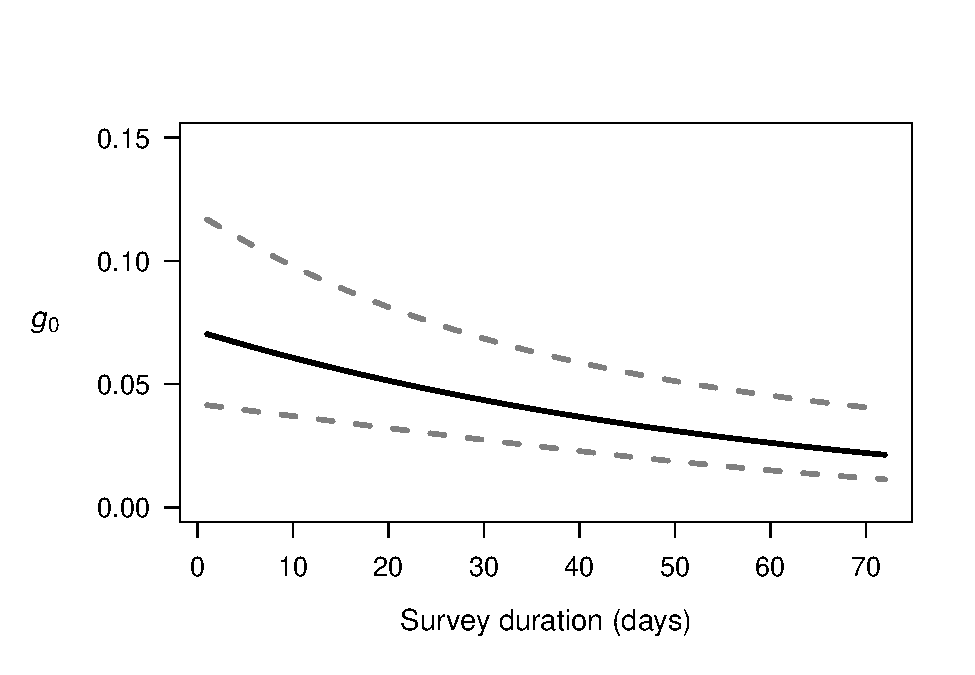
\includegraphics[width=0.7\linewidth]{figure/otways17-g0t-1} 

}

\caption{The AICc-best model linear trend in \textit{g}0 values (probability of daily detection in activity centre) throughout the survey. Grey dashed lines indicate 95\% confidence intervals.}\label{fig:otways17-g0t}
\end{figure}
\newpage

\(~\)

\(~\)

\(~\)

\begingroup\fontsize{10}{12}\selectfont
\begin{longtable}[t]{lrrrrrrr}
\caption{\label{tab:otways17-detfn}Model selection table and density estimates for different detection function shapes for spatial mark-resight models.}\\
\toprule
\multicolumn{5}{c}{Model comparison} & \multicolumn{3}{c}{Density estimate (cats km-2)} \\
\cmidrule(l{3pt}r{3pt}){1-5} \cmidrule(l{3pt}r{3pt}){6-8}
Detector function & K & AICc & dAICc & AICcwt & estimate & lcl & ucl\\
\midrule
\endfirsthead
\caption[]{\label{tab:otways17-detfn}Model selection table and density estimates for different detection function shapes for spatial mark-resight models. \textit{(continued)}}\\
\toprule
\multicolumn{5}{c}{Model comparison} & \multicolumn{3}{c}{Density estimate (cats km-2)} \\
\cmidrule(l{3pt}r{3pt}){1-5} \cmidrule(l{3pt}r{3pt}){6-8}
Detector function & K & AICc & dAICc & AICcwt & estimate & lcl & ucl\\
\midrule
\endhead

\endfoot
\bottomrule
\multicolumn{8}{l}{\rule{0pt}{1em}K - number of parameters}\\
\multicolumn{8}{l}{\rule{0pt}{1em}AICc - Akaike's Information Criterion with small-sample adjustment}\\
\multicolumn{8}{l}{\rule{0pt}{1em}dAICc - difference between AICc of this model and the model with smallest AICc}\\
\multicolumn{8}{l}{\rule{0pt}{1em}AICcwt - AICc model weight}\\
\multicolumn{8}{l}{\rule{0pt}{1em}lcl – lower 95\% confidence limit}\\
\multicolumn{8}{l}{\rule{0pt}{1em}ucl – upper 95\% confidence limit}\\
\endlastfoot
hazard-rate & 4 & 2359.59 & 0.00 & 0.7 & 1.15 & 0.93 & 1.42\\
exponential & 3 & 2361.25 & 1.66 & 0.3 & 1.19 & 0.96 & 1.49\\
halfnormal & 3 & 2373.30 & 13.72 & 0.0 & 1.12 & 0.93 & 1.35\\*
\end{longtable}
\endgroup{}

\hypertarget{occ-app}{%
\chapter{Supporting Information: Chapter \ref{occ}}\label{occ-app}}

\newpage

\begingroup\fontsize{10}{12}\selectfont
\begin{longtable}[t]{llrrrrrr}
\caption{\label{tab:occ-naive}Number of camera-trap sites, total deployments and naive occupancy rates for red foxes, feral cats, southern brown bandicoots (SBB) and long-nosed potoroos (LNP) within Ecological Vegetation Class groups across two broad regions in south-west Victoria, Australia.}\\
\toprule
Vegetation & Region & Sites & Deployments & Fox & Cat & SBB & LNP\\
\midrule
Dry Forest & Glenelg & 25 & 69 & 0.65 & 0.10 & 0.06 & 0.01\\
 & Otway & 111 & 314 & 0.42 & 0.28 & 0.02 & 0.06\\
Heathland & Glenelg & 40 & 119 & 0.43 & 0.34 & 0.14 & 0.18\\
 & Otway & 3 & 9 & 0.22 & 0.44 & 0.11 & 0.33\\
Heathy Woodland & Glenelg & 154 & 424 & 0.31 & 0.14 & 0.29 & 0.19\\
\addlinespace
 & Otway & 82 & 255 & 0.29 & 0.15 & 0.15 & 0.12\\
Herb-rich Woodland & Glenelg & 59 & 373 & 0.50 & 0.27 & 0.02 & 0.12\\
 & Otway & 2 & 6 & 0.33 & 0.17 & 0.00 & 0.00\\
Lowland Forest & Glenelg & 383 & 1046 & 0.46 & 0.18 & 0.17 & 0.05\\
 & Otway & 52 & 163 & 0.42 & 0.14 & 0.04 & 0.10\\
\addlinespace
Swampy Scrub & Glenelg & 4 & 10 & 0.60 & 0.50 & 0.00 & 0.00\\
 & Otway & 36 & 98 & 0.32 & 0.33 & 0.08 & 0.09\\
Wet Forest & Otway & 281 & 780 & 0.31 & 0.54 & 0.01 & 0.07\\
\bottomrule
\end{longtable}
\endgroup{}

\newpage
\begin{figure}

{\centering 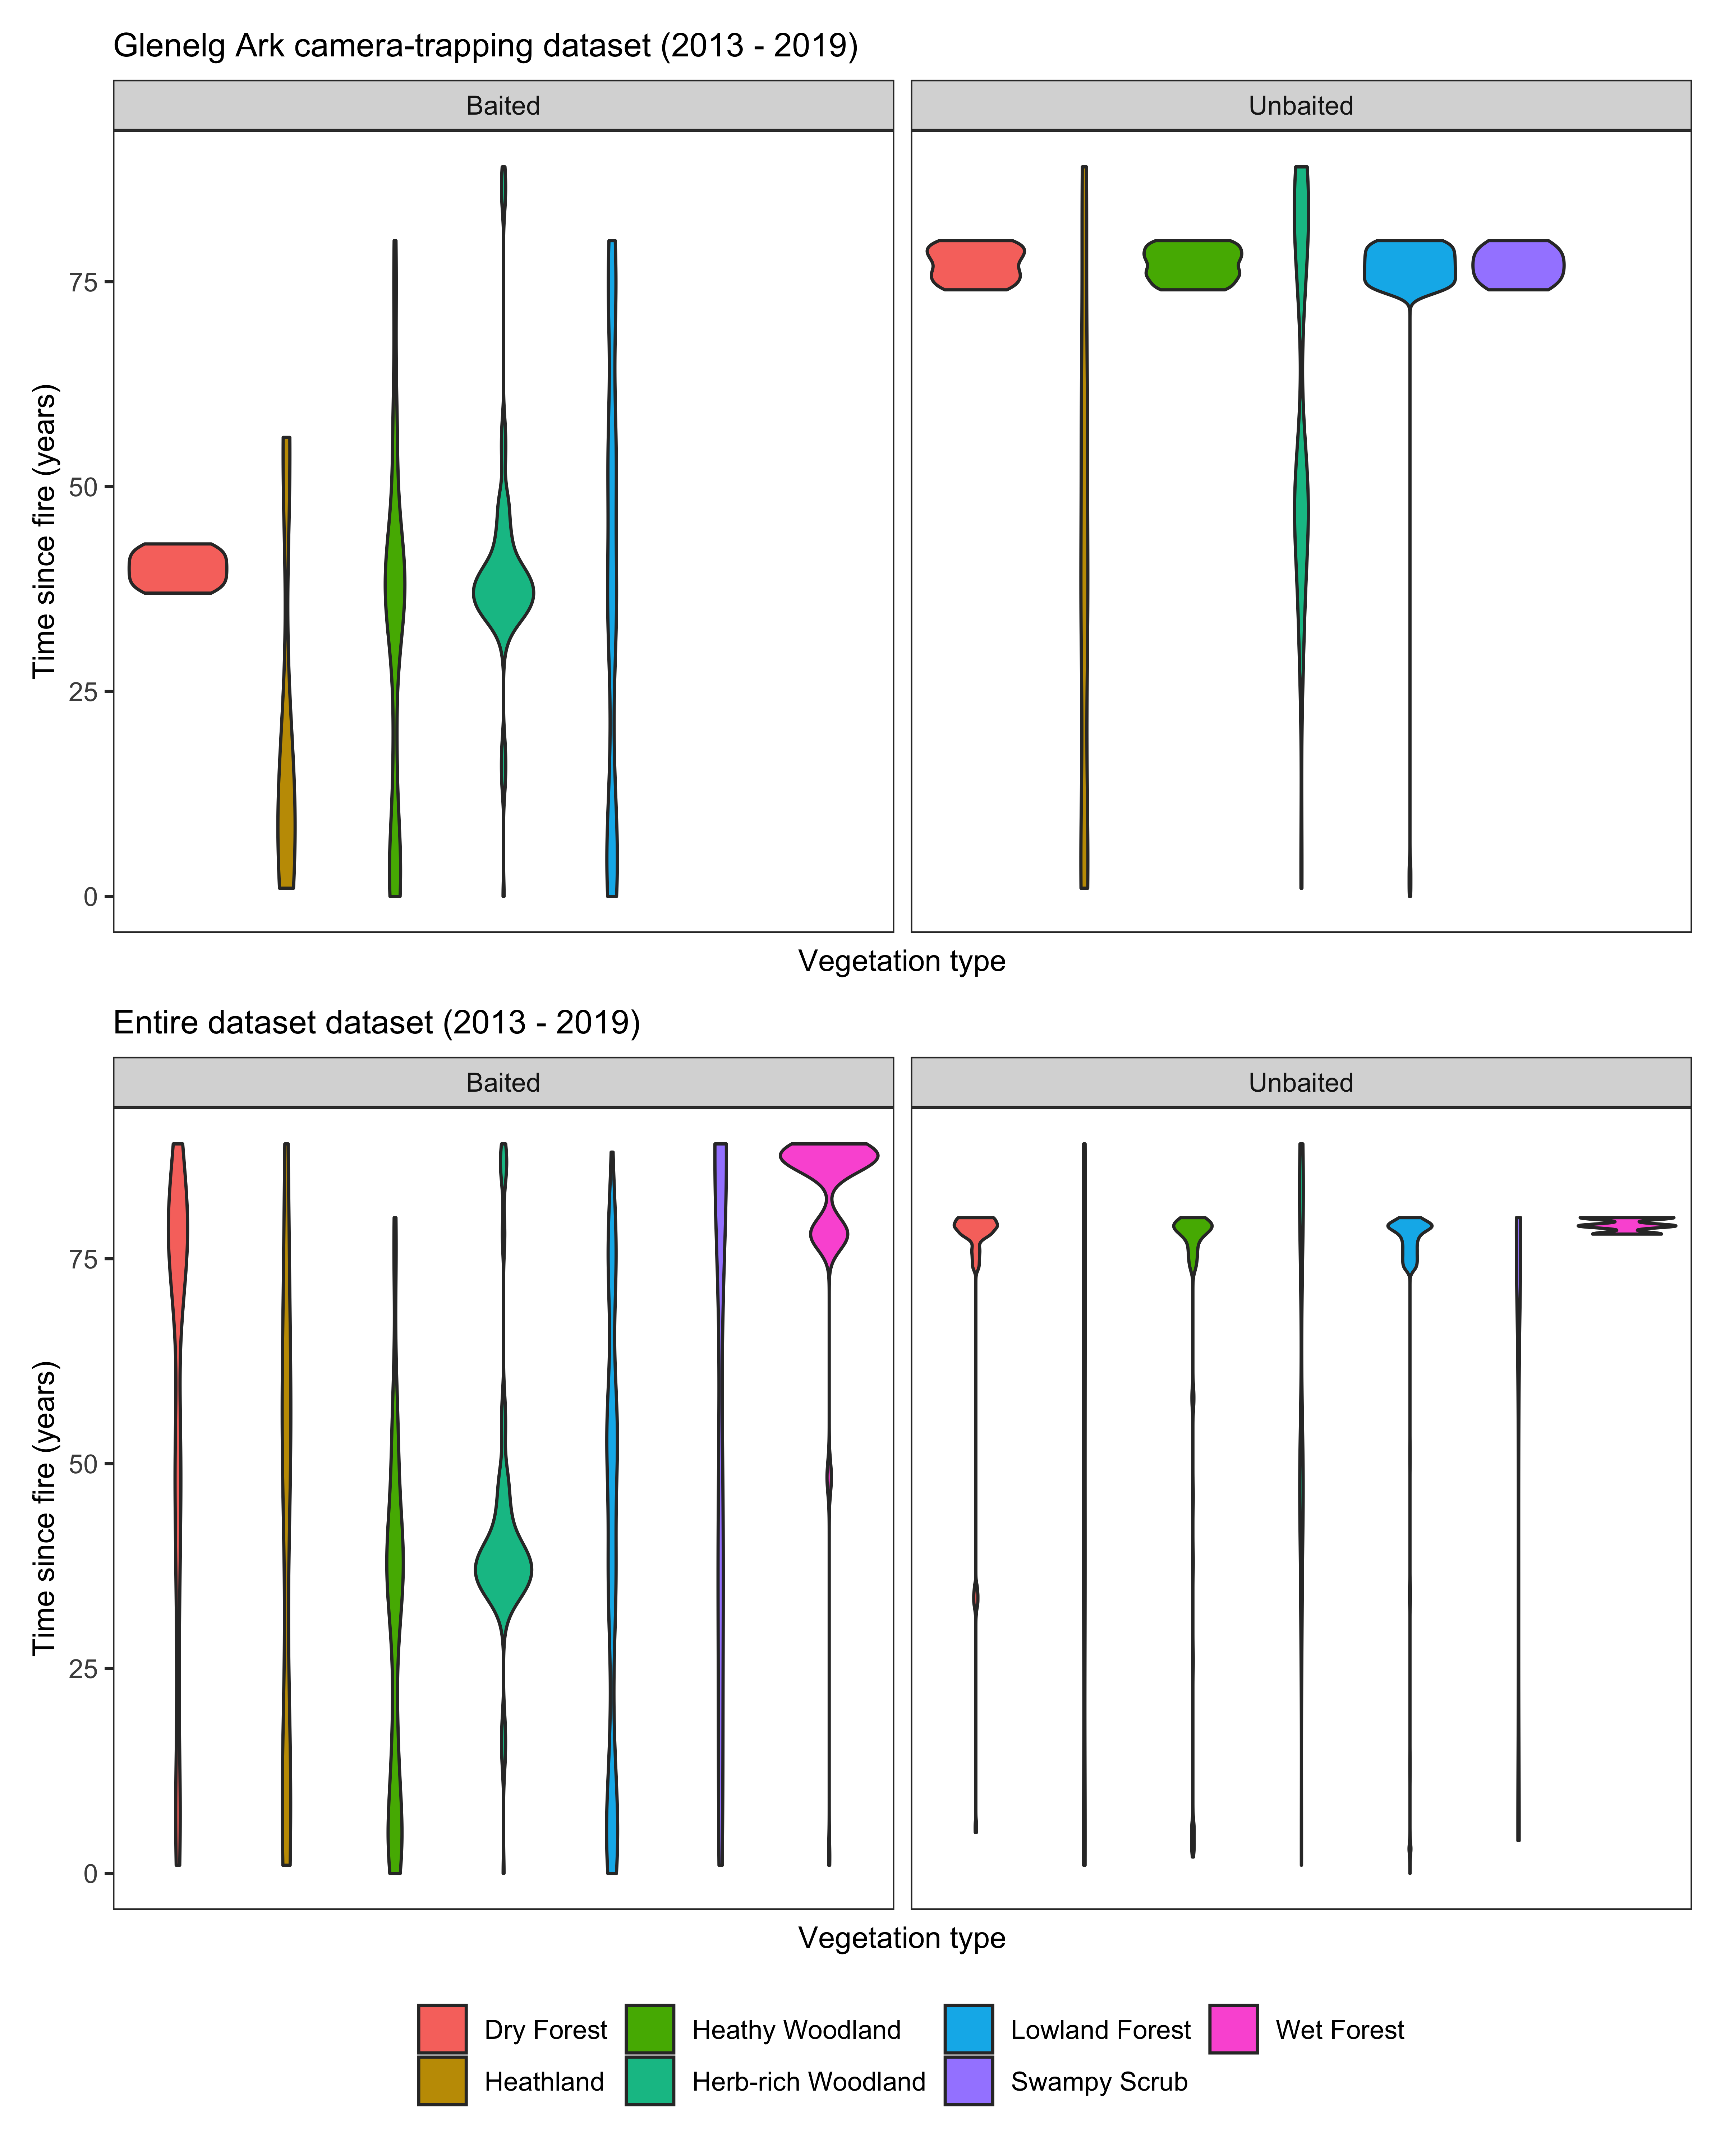
\includegraphics[width=1\linewidth]{figure/raw_data_tsf_veg} 

}

\caption{Range and distribution of time since fire values across the surveyed vegetation types in baited and unbaited sites. In the Glenelg Ark camera-trapping dataset, where most sites in the baited landscapes are relatively recently burnt, and most sites are long-unburnt in the unbaited landscapes. Combining M.W.R PhD and Otway Ark surveys provides a wider range of fire history patterns in each vegetation type with and without fox control.}\label{fig:veg-tsf-violin}
\end{figure}
\newpage
\begin{figure}

{\centering 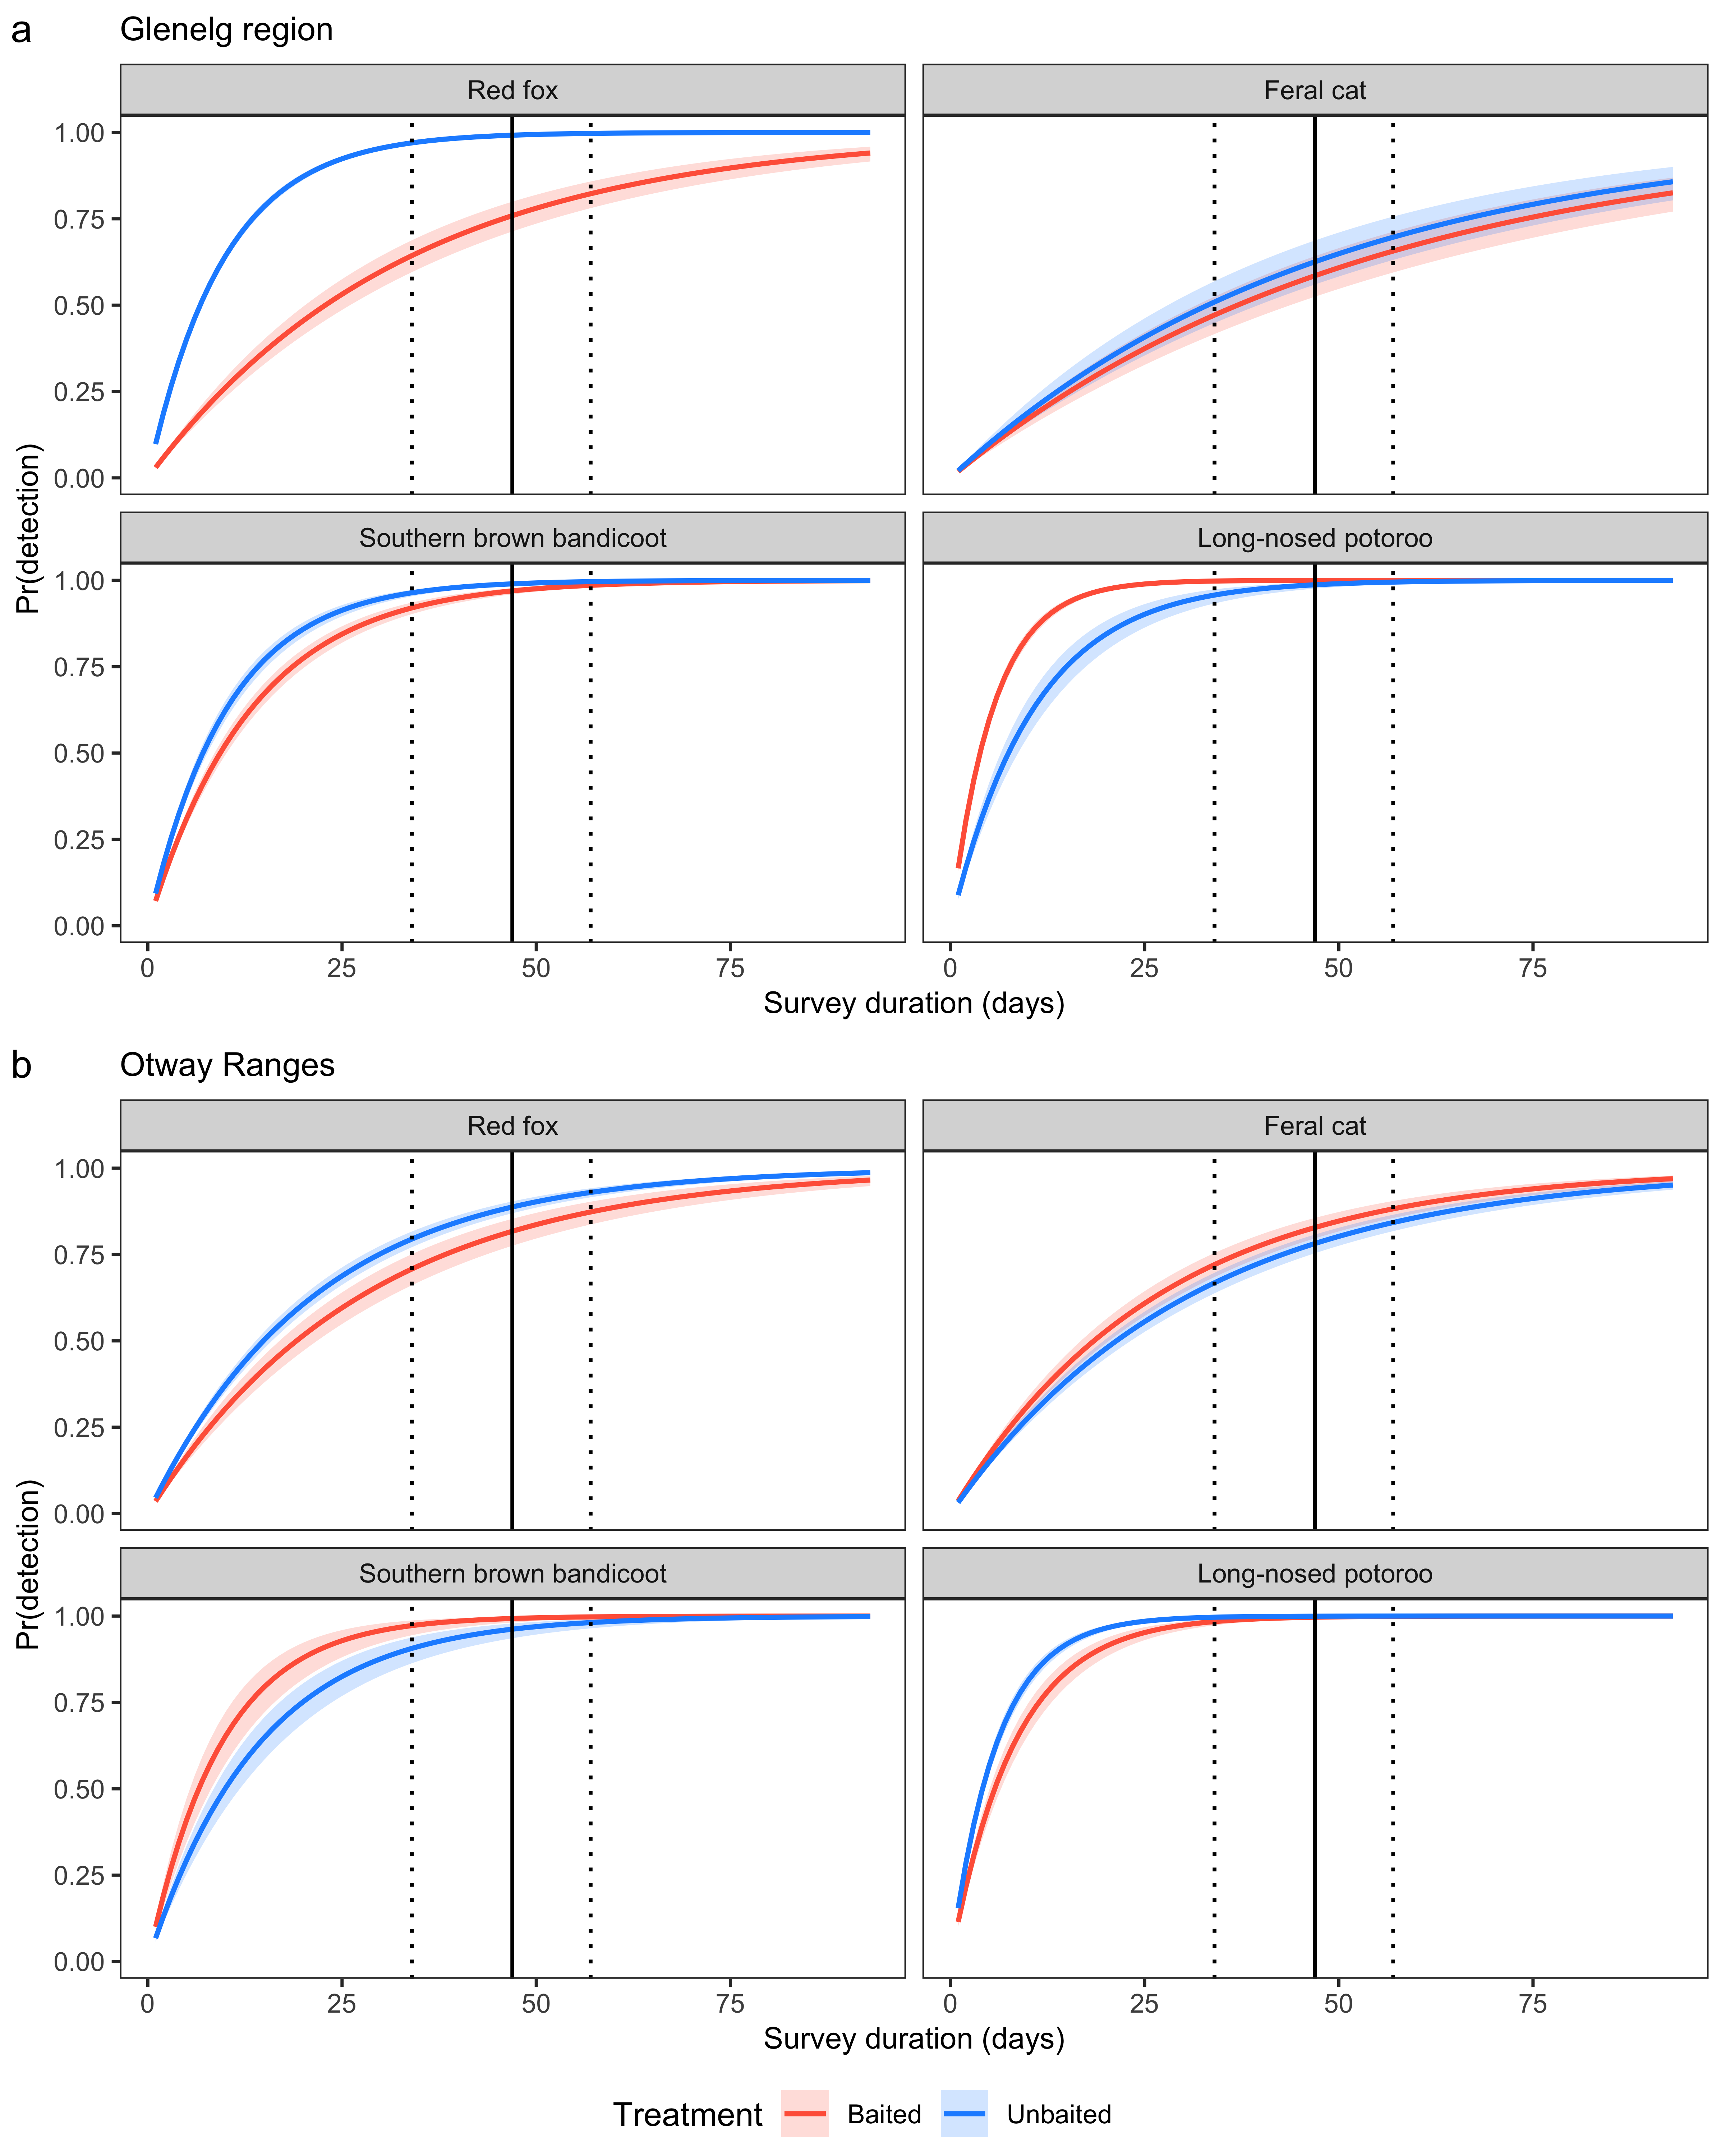
\includegraphics[width=1\linewidth]{figure/cumulative_detectability} 

}

\caption{Cumulative detection probabilities of species in landscapes with fox control (red) and without fox control (blue) in the Glenelg region (a) and Otway Ranges, south-west Victoria, Australia. Fox control had occurred in The Glenelg region for 8 - 13 years and was monitored with a control-impact design. The Otway Ranges was monitored using a before-after-control-impact experimental design; surveyed approximately 1 year prior and 2 years following the commencement of fox-baiting. Vertical grey lines represent mean (solid) as well as 25\% and 75\% quantiles (dotted) of days camera-traps were active for. Shaded bands represent 95\% Bayesian credible intervals. Estimates derived from Bayesian occupancy-detection models.}\label{fig:occ-cumdet}
\end{figure}
\newpage

\begingroup\fontsize{10}{12}\selectfont
\begin{longtable}[t]{lrrr}
\caption{\label{tab:occ-rain-aic}Akaike's Information Criterion values for generalised additive models with different rainfall periods.}\\
\toprule
Species & Months & AIC & dAIC\\
\midrule
Red fox & 6 & 4150.14 & 0.00\\
Red fox & 18 & 4151.57 & 1.43\\
Red fox & 24 & 4156.49 & 6.35\\
Red fox & 12 & 4158.20 & 8.06\\
Feral cat & 6 & 3732.68 & 0.00\\
\addlinespace
Feral cat & 12 & 3733.39 & 0.71\\
Feral cat & 18 & 3733.39 & 0.71\\
Feral cat & 24 & 3733.39 & 0.71\\
Southern brown bandicoot & 6 & 1868.55 & 0.00\\
Southern brown bandicoot & 24 & 1868.56 & 0.00\\
\addlinespace
Southern brown bandicoot & 18 & 1874.10 & 5.54\\
Southern brown bandicoot & 12 & 1877.49 & 8.94\\
Long-nosed potoroo & 12 & 1577.71 & 0.00\\
Long-nosed potoroo & 18 & 1581.19 & 3.48\\
Long-nosed potoroo & 24 & 1581.34 & 3.62\\
\addlinespace
Long-nosed potoroo & 6 & 1582.96 & 5.25\\
\bottomrule
\multicolumn{4}{l}{\rule{0pt}{1em}\textit{Note: }}\\
\multicolumn{4}{l}{\rule{0pt}{1em}AIC - Akaike's Information Criterion score}\\
\multicolumn{4}{l}{\rule{0pt}{1em}dAIC - difference between AIC of this model and the model with smallest AIC}\\
\end{longtable}
\endgroup{}

\newpage

\begingroup\fontsize{10}{12}\selectfont
\begin{longtable}[t]{llrrrr}
\caption{\label{tab:occ-model-sumstats}Generalised additive model summary statistics for models with 'full' set of explanatory variables relative to a 'null model' with only a site random effect.}\\
\toprule
Species & Model & EDF & dev.expl & r.sq & AIC\\
\midrule
Red fox & null & 420.65 & 0.28 & 0.27 & 4392.19\\
Red fox & full & 240.21 & 0.26 & 0.27 & 4150.14\\
Feral cat & null & 300.15 & 0.24 & 0.22 & 3901.10\\
Feral cat & full & 214.76 & 0.24 & 0.24 & 3732.68\\
Southern brown bandicoot & null & 242.65 & 0.36 & 0.27 & 2079.84\\
\addlinespace
Southern brown bandicoot & full & 185.37 & 0.40 & 0.32 & 1868.55\\
Long-nosed potoroo & null & 280.29 & 0.50 & 0.45 & 1671.09\\
Long-nosed potoroo & full & 256.45 & 0.53 & 0.47 & 1577.71\\
\bottomrule
\multicolumn{6}{l}{\rule{0pt}{1em}\textit{Note: }}\\
\multicolumn{6}{l}{\rule{0pt}{1em}EDF - estimated degrees of freedom of all model terms.}\\
\multicolumn{6}{l}{\rule{0pt}{1em}dev.expl - proportion of the null deviance explained by the model. }\\
\multicolumn{6}{l}{\rule{0pt}{1em}r.sq -  adjusted r-squared value.}\\
\multicolumn{6}{l}{\rule{0pt}{1em}AIC - Akaike's Information Criterion score}\\
\end{longtable}
\endgroup{}

\newpage
\begin{figure}

{\centering 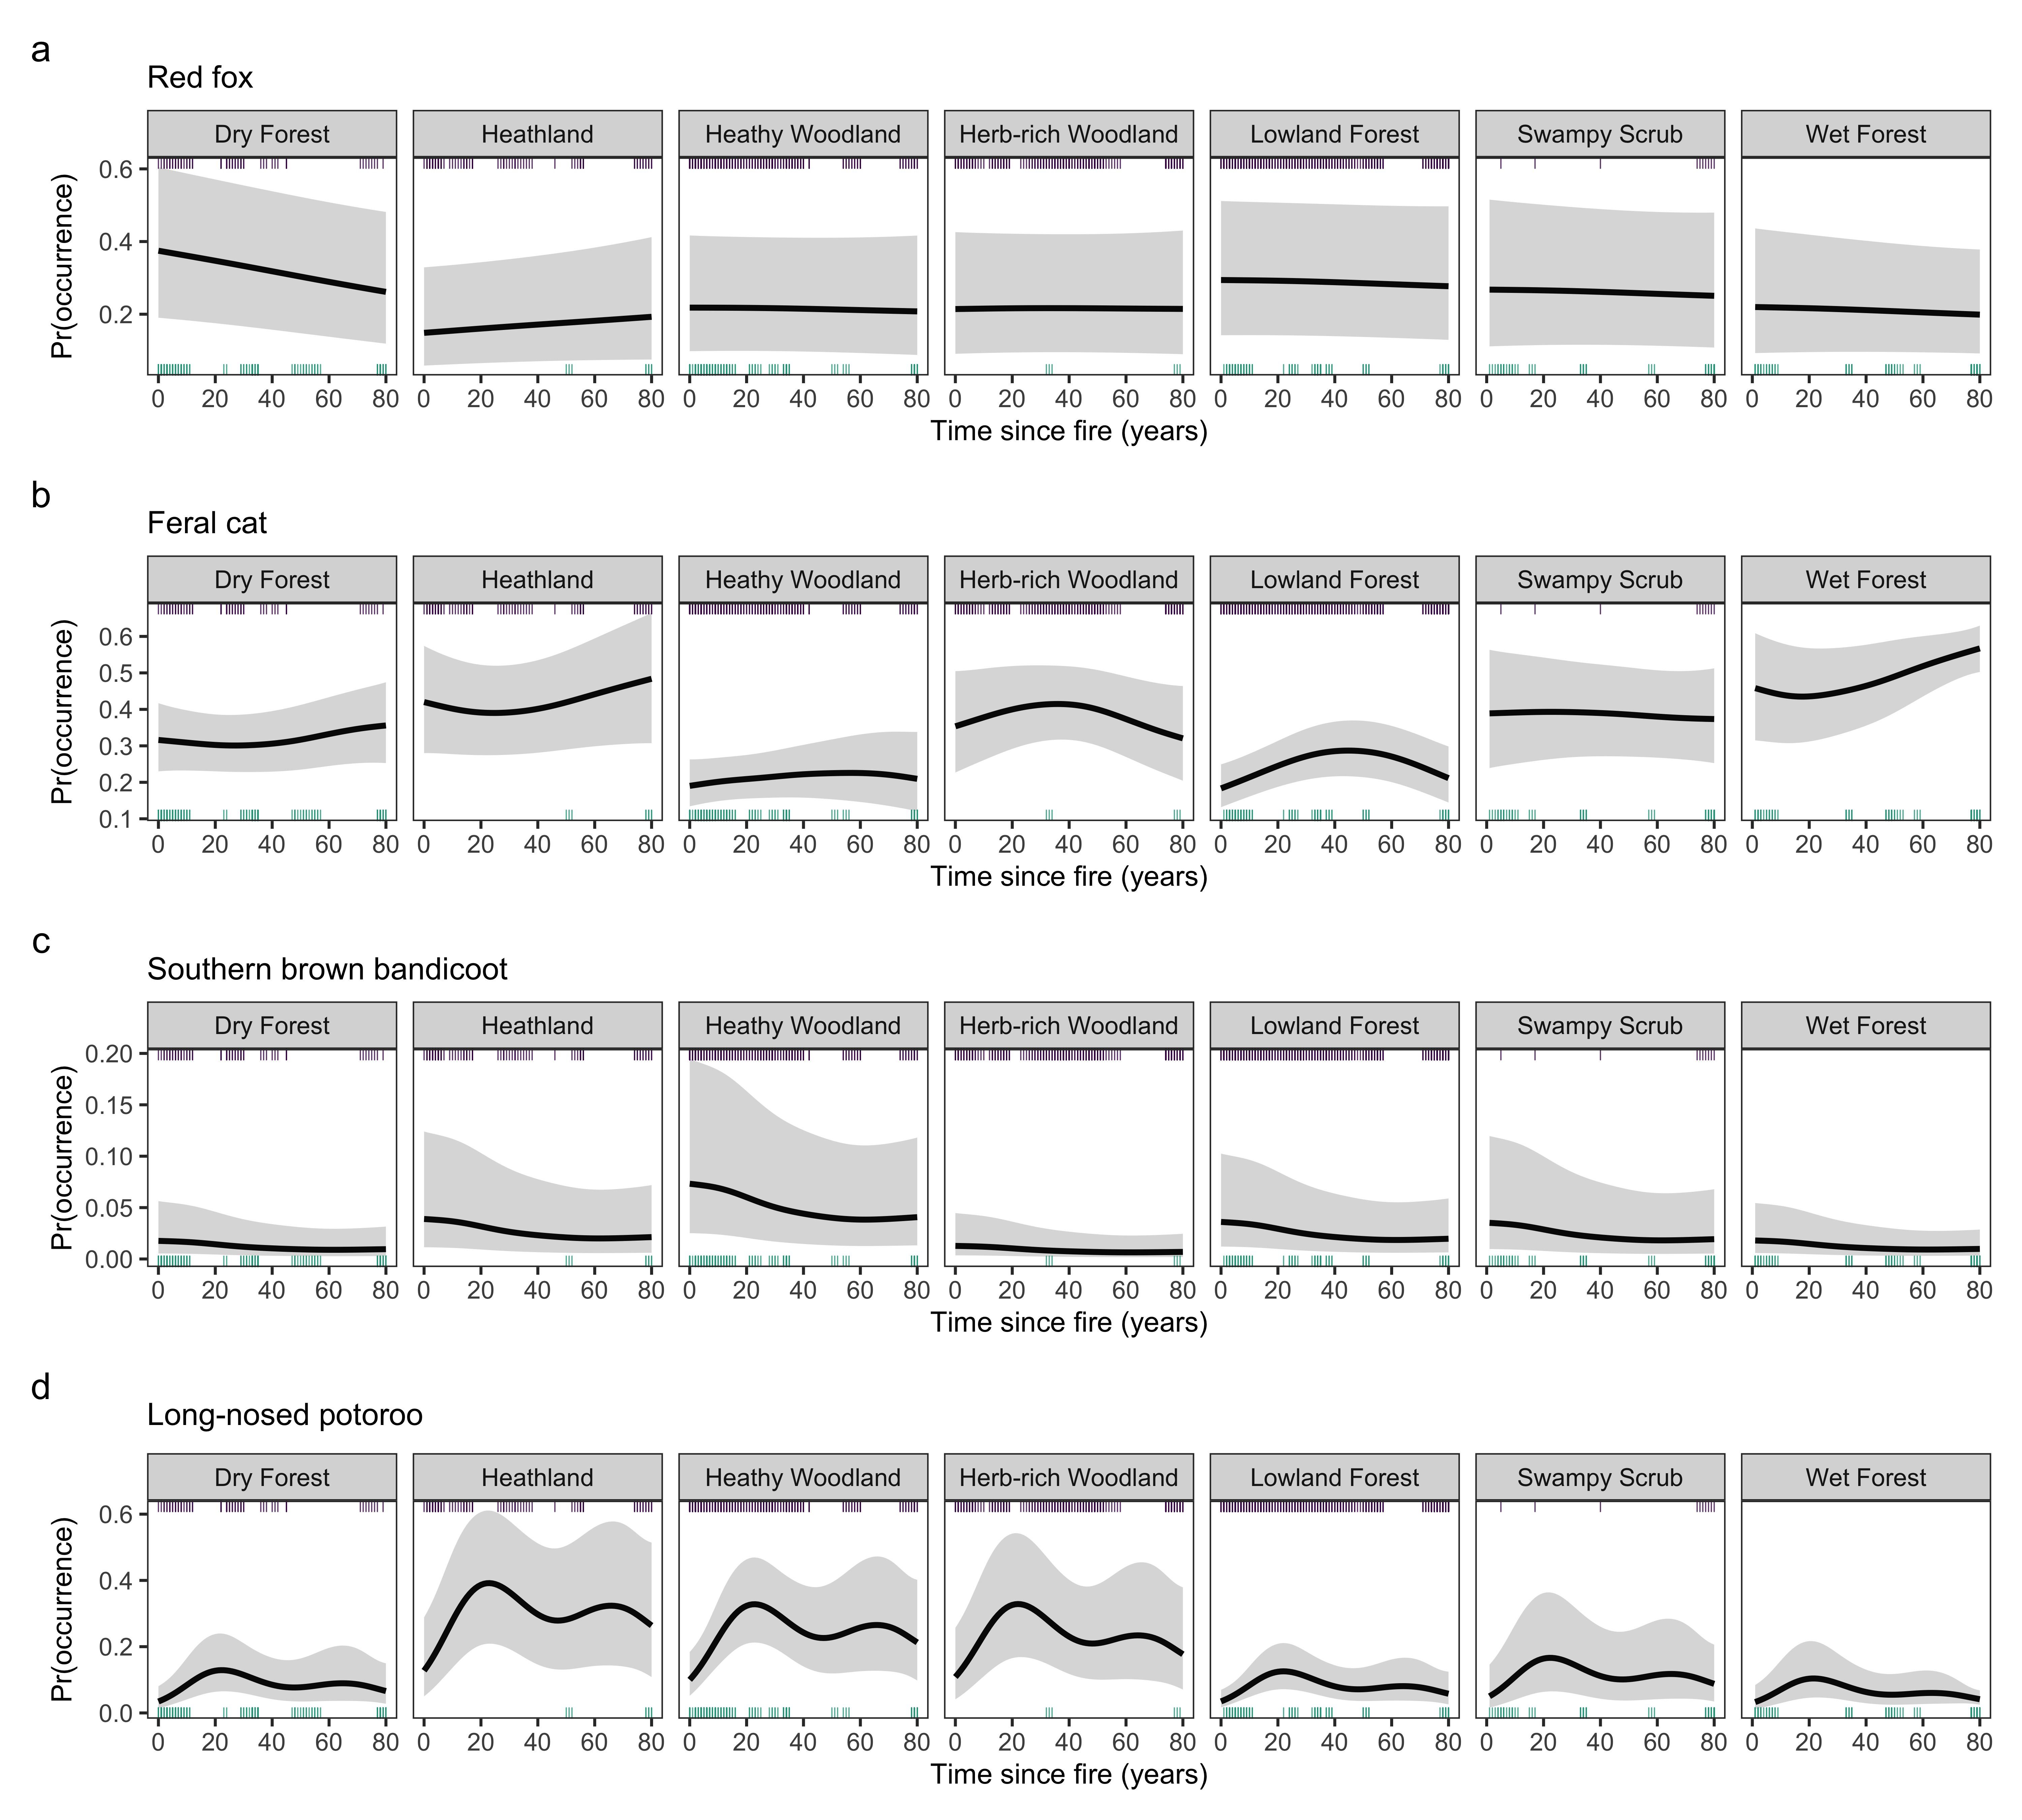
\includegraphics[width=1\linewidth]{figure/tsf} 

}

\caption{Time since fire had a weak impact on fox (a) and feral cat (b) occupancy probability in south-west Victoria, Australia. Southern brown bandicoot occupancy probability (c) peaked around 15 and 75 years following fire, although, the magnitude of both peaks differed across Ecological Vegetation Class groups. Long-nosed potoroo occupancy probability (d) linearly increased with time since fire in heathy vegetation groups, but linearly decreased with years post-fire in Herb-Rich Woodlands. Estimates derived from generalised additive models (assuming perfect detection). Shaded regions indicate 95\% confidence intervals. Rug ticks representing the distribution of time since fire data for the Glenelg region (brown) is shown on the inside of the top axis, Otway Ranges distribution shown on the inside of the bottom axis (navy).}\label{fig:occ-tsf}
\end{figure}
\hypertarget{density-app}{%
\chapter{Supporting Information: Chapter \ref{density}}\label{density-app}}

\newpage

\hypertarget{density-app-field}{%
\section{Field surveys}\label{density-app-field}}

In the Glenelg region, we deployed camera-traps once at a unique sites once. In the Otway region, we redeployed camera-traps in sites annually for three years. All 2017 camera-sites were resurveyed each year, except for four logistically challenging sites in the southern grid. In 2018, we added 16 additional sites in the southern grid, as well as 36 additional sites in the northern grid. These additional sites were resurveyed in 2019.

At each site, we deployed a single Reconyx (Holmen, Wisconsin) branded camera-trap with passive infrared sensor that detects a thermal differential between the subject and the background temperature. The majority of camera-traps were Reconyx Hyperfire HC600 (97\% in the Glenelg region; 78\% in the Otway Ranges); in the Glenelg region PC900's were deployed in the remained of sites (3\%), whereas in the Otway Ranges PC900, PC800, HC500 and HF2X models were also used (Table \ref{tab:cam-models}). We programmed camera's to high sensitivity and to take five consecutive photographs when triggered (no quiet period). We attached each camera to a tree, approximately 30 cm above the ground, and facing toward a lure 2 - 2.5 m away. The lure comprised an oil-absorbing cloth doused in tuna oil and placed inside a PVC pipe container with a mesh top. We secured each lure to the top of a 1 m wooden stake and attached a handful of small white feathers to the outside of the PVC pipe container. Feathers were not used in the Lower Glenelg National Park survey. We cleared vegetation in the camera's line-of-sight to reduce false triggers and avoid obscuring cat coat markings in images.

\newpage

\(~\)

\(~\)

\(~\)
\begin{figure}

{\centering 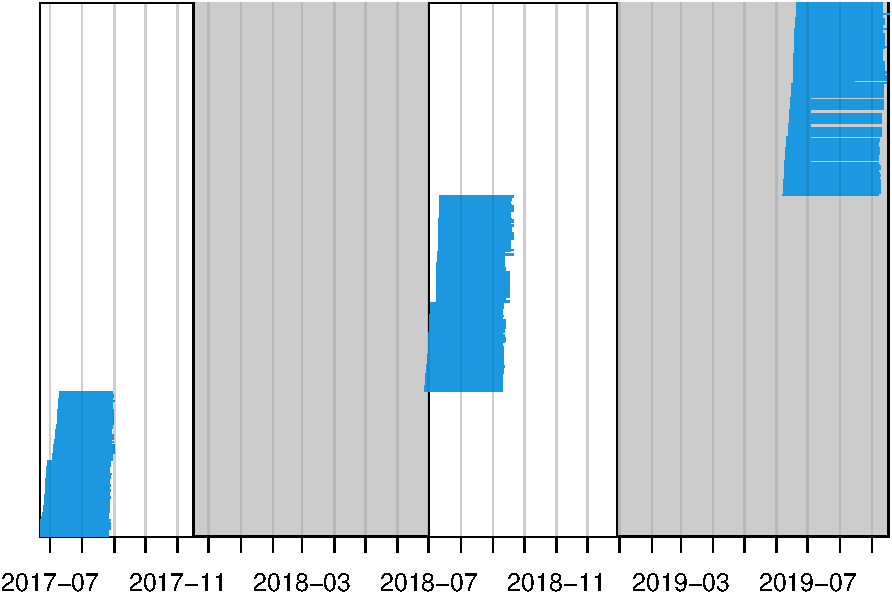
\includegraphics[width=1\linewidth]{figure/density-camop-1} 

}

\caption{Camera-trap operation times in the Otway region, Australia. Each blue horizontal line represents one camera-trap deployment. Grey shading indicates periods of fox control in the impact landscape.}\label{fig:density-camop}
\end{figure}
\newpage

\newpage
\begingroup\fontsize{10}{12}\selectfont
\begin{longtable}[t]{lllllllr}
\caption{\label{tab:tab-dates}Survey dates of camera-trapping grids and naive occurrence rates of foxes (proportion of camera-traps foxes were detected at) in each surveyed landscape}\\
\toprule
Region & Landscape & Replicate & Year & Date start & Date end & Duration & Naive fox occurrence\\
\midrule
\endfirsthead
\caption[]{\label{tab:tab-dates}Survey dates of camera-trapping grids and naive occurrence rates of foxes (proportion of camera-traps foxes were detected at) in each surveyed landscape \textit{(continued)}}\\
\toprule
Region & Landscape & Replicate & Year & Date start & Date end & Duration & Naive fox occurrence\\
\midrule
\endhead

\endfoot
\bottomrule
\endlastfoot
Glenelg & Annya & 1 & 2018 & 2018-01-26 & 2018-04-13 & 76 days & 0.55\\
Glenelg & Cobboboonee & 1 & 2018 & 2018-02-13 & 2018-04-29 & 74 days & 0.26\\
Glenelg & Hotspur & 2 & 2018 & 2018-04-16 & 2018-06-21 & 65 days & 0.48\\
Glenelg & Mt Clay & 2 & 2018 & 2018-04-30 & 2018-06-27 & 57 days & 0.35\\
Glenelg & LGNP South & 3 & 2021 & 2021-03-25 & 2021-05-12 & 47 days & 0.17\\
\addlinespace
Glenelg & LGNP North & 3 & 2021 & 2021-03-30 & 2021-05-14 & 44 days & 0.57\\
Otway & South & 1 & 2017 & 2017-06-23 & 2017-08-30 & 67 days & 0.36\\
Otway & North & 1 & 2017 & 2017-07-05 & 2017-09-02 & 58 days & 0.13\\
Otway & South & 2 & 2018 & 2018-06-28 & 2018-09-13 & 76 days & 0.27\\
Otway & North & 2 & 2018 & 2018-07-09 & 2018-09-21 & 73 days & 0.27\\
\addlinespace
Otway & South & 3 & 2019 & 2019-06-07 & 2019-09-17 & 101 days & 0.17\\
Otway & North & 3 & 2019 & 2019-06-13 & 2019-09-15 & 93 days & 0.43\\*
\end{longtable}
\endgroup{}

\newpage

\begingroup\fontsize{10}{12}\selectfont
\begin{longtable}[t]{llr}
\caption{\label{tab:cam-models}Frequency of different Reconyx camera-trap models used in each survey}\\
\toprule
Region & Camera model & Frequency\\
\midrule
\endfirsthead
\caption[]{\label{tab:cam-models}Frequency of different Reconyx camera-trap models used in each survey \textit{(continued)}}\\
\toprule
Region & Camera model & Frequency\\
\midrule
\endhead

\endfoot
\bottomrule
\endlastfoot
Glenelg & HC600 HYPERFIRE & 413\\
Glenelg & PC900 PROFESSIONAL & 12\\
Otway & HC500 HYPERFIRE & 9\\
Otway & HC600 HYPERFIRE & 405\\
Otway & HYPERFIRE 2 COVERT & 59\\
\addlinespace
Otway & PC800 PROFESSIONAL & 6\\
Otway & PC900 PROFESSIONAL & 34\\*
\end{longtable}
\endgroup{}

\newpage
\begin{figure}

{\centering 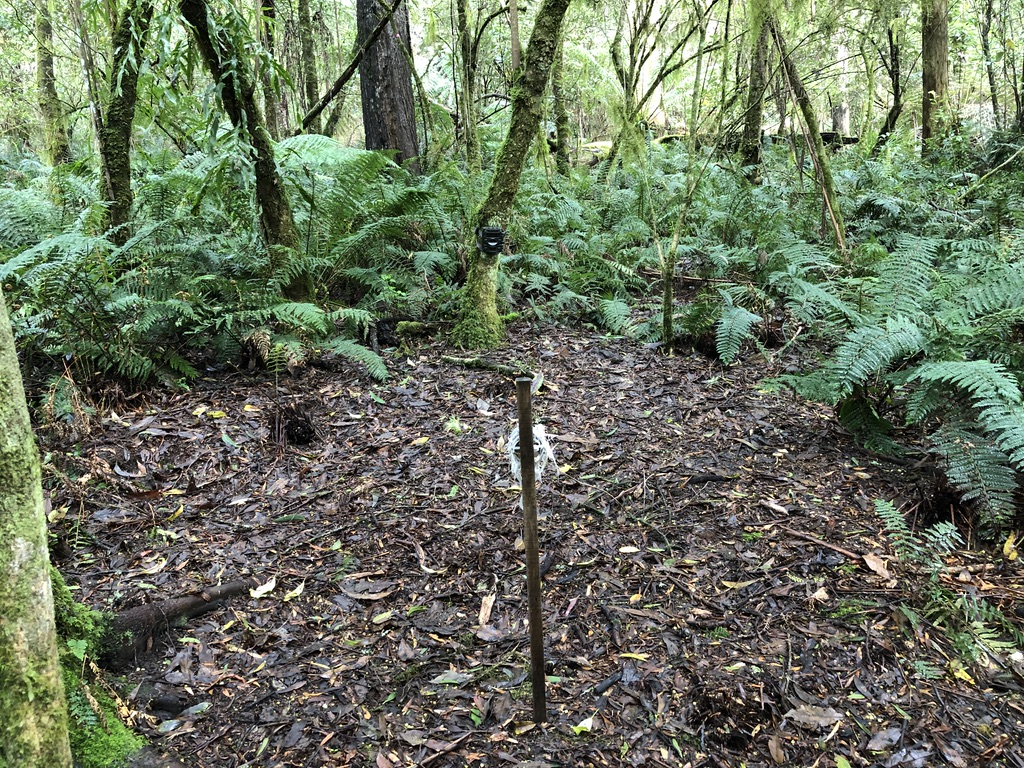
\includegraphics[width=1\linewidth]{figure/camtrap1} 

}

\caption{Example of a typical camera-trap set-up in the Otway region, Australia.}\label{fig:density-cam-photo}
\end{figure}
\newpage

\hypertarget{density-app-id}{%
\section{Individual cat identification}\label{density-app-id}}

We first labelled every camera-trap image with a species metadata tag using \href{https://www.digikam.org}{DigiKam software}. We also added metadata tags for each cat coat type: black, mackerel / spotted tabby, classic tabby, ginger and other (coats with multiple colour blends; Fig. 3). This allowed us to summarise species records and extract cat images using the `camtrapR' R-package (Niedballa \emph{et al.} 2016).

We considered all black cats to be of the `unmarked' category in spatial mark-resight models - even the few with white splotches on their underside (as these couldn't always be seen as cats move with their head down).

In the remaining coat categories where possible, we identified individual cats based on their unique coat markings. The ability to identify individuals substantially increased as the image library for each cat increased. Therefore we made the easiest identifications first to build up these libraries, before making decisions on the less obvious detections. We examined and matched all coat markings seen between two particular detections. Markings on the front legs were the most useful for ID's as the patterns do not skew as much with different body positions. On the whole, unidentifiable detections were mainly due to only part of a cat appearing in the frame, or because photos were blurry (because of cat movement or a foggy camera lens).

We were left with a small number of instances (less than ten) where only left or right flanks could be seen. In this case, the side with the most repeat detections was labelled as an individual, whereas the side with the least number of detections was considered unidentifiable. Additionally, an extremely small portion of cats in the Otways had ginger coats. When ginger coats are photographed with an infrared flash, they become overexposed and no markings can be seen (see the image in bottom-right corner in Fig. S3). Therefore, if there were multiple ginger cat detections in a single grid, we treated them in the same way as one-sided flank detections.

One observer identified the 2018 feral cats in the Glenelg region (MR) and the 2021 Lower Glenelg National Park cats (Luke Woodford). In the 2017 and 2018 Otway datasets (where there were substantially more cat detections and fewer distinct coat patterns) two independent observers identified individual cats and discrepancies between observers were reviewed together until consensus was reached (MR, MLP, BH). If no consensus was reached, the cat was considered unidentifiable. In the 2019 Otway dataset, many of the identified cats were sighted in the previous surveys -- these larger individual libraries meant that cats could be identified more easily so only one observer was necessary (MR). We also identified individual cats in additional camera-trap surveys taken within the Otway region grids (just before each of our surveys) using white flash camera-traps (Zoï Banikos, unpublished data), providing additional images of individuals in the photo library for identifications.

We were therefore left with three groups of cats: unmarked (black cats), marked (cats which could be identified to the individual-level with complete certainty) and mark status unknown (cats which were not black, but couldn't be identified to the individual level with complete certainty).

We ignored the few detections of cats which were obviously young enough to be dependent on a parent, as these kittens do not have independent activity centres or movements and were not yet recruited into the adult population.

\newpage

\(~\)

\(~\)

\(~\)
\begin{figure}

{\centering 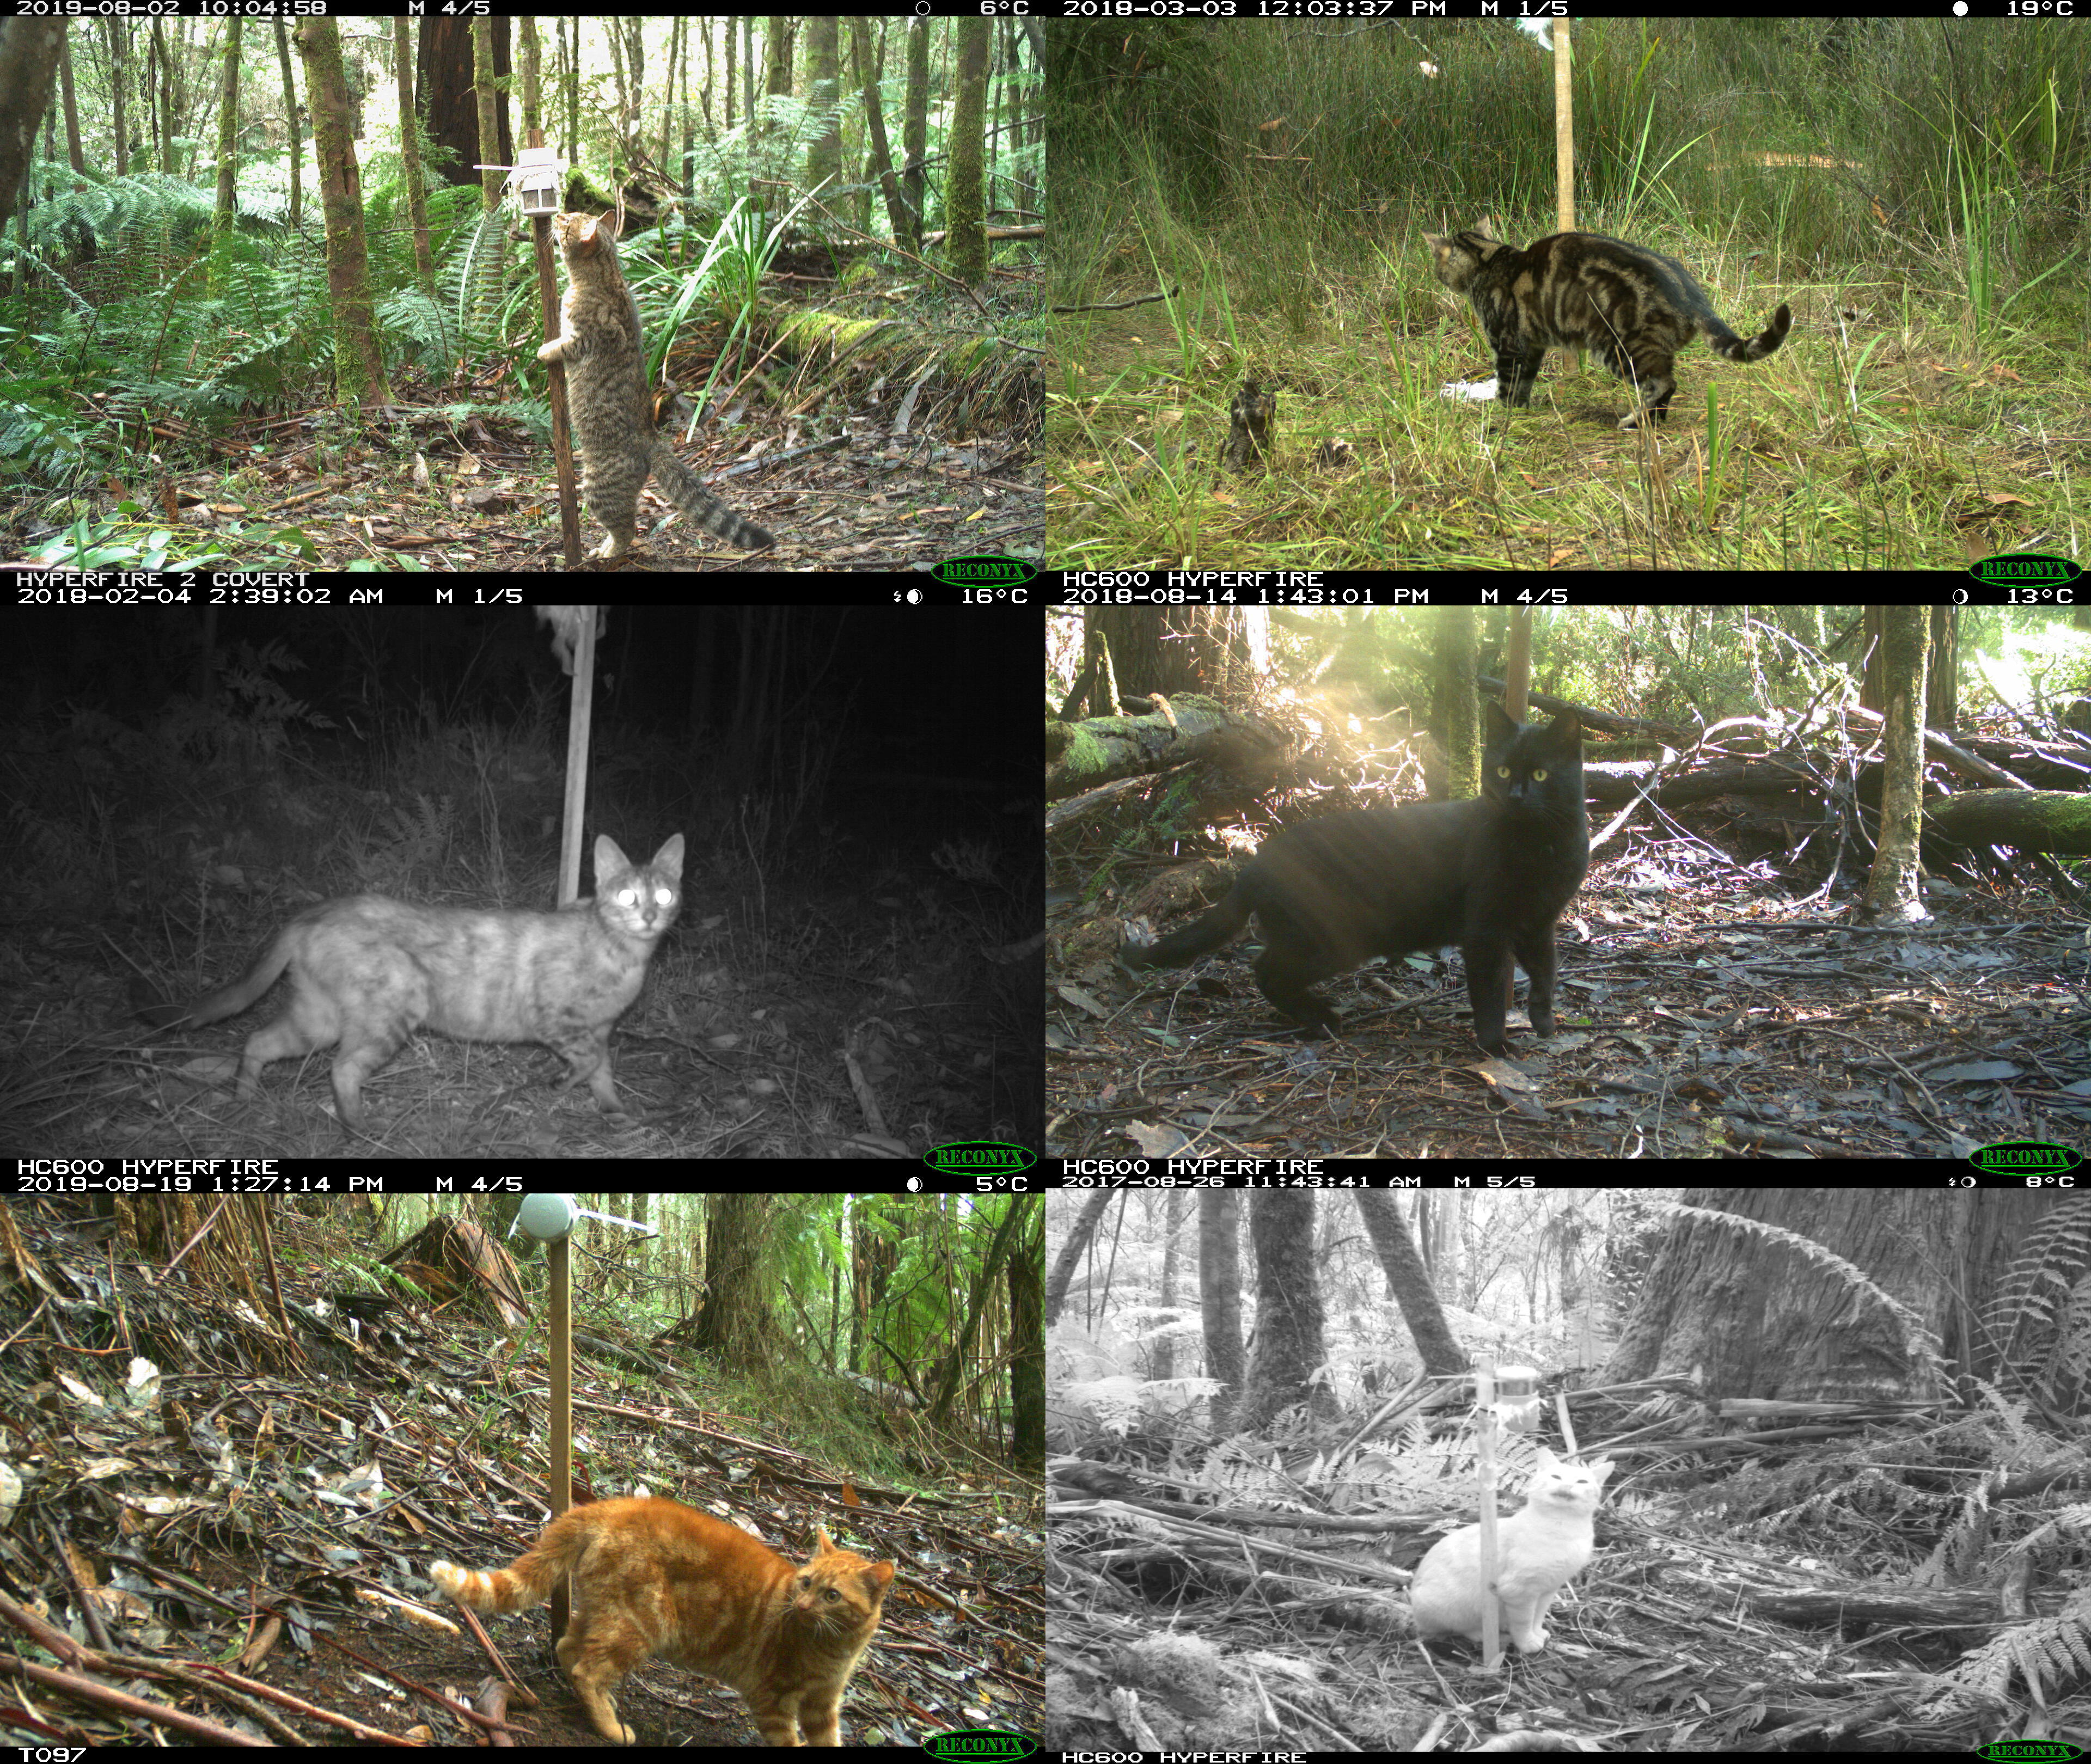
\includegraphics[width=1\linewidth]{figure/cat_coats} 

}

\caption{Feral cat coat categories from left-right, top-bottom: mackerel / spotted tabby, classic tabby, other, black, ginger and ginger with infrared flash.}\label{fig:density-cat-photo}
\end{figure}
\newpage

\hypertarget{summary-statistics}{%
\section{Summary statistics}\label{summary-statistics}}

\(~\)

\(~\)

\(~\)

\begingroup\fontsize{10}{12}\selectfont
\begin{longtable}[t]{lrrrrrrr}
\caption{\label{tab:density-stats}Summary of camera-trap survey effort and feral cat detections.}\\
\toprule
\multicolumn{5}{c}{ } & \multicolumn{3}{c}{Detections (max. 1 per 24-hr)} \\
\cmidrule(l{3pt}r{3pt}){6-8}
Landscape & Cameras & Trapnights & Cats & Moves & Identified & Unidentified & Unmarked\\
\midrule
\endfirsthead
\caption[]{\label{tab:density-stats}Summary of camera-trap survey effort and feral cat detections. \textit{(continued)}}\\
\toprule
\multicolumn{5}{c}{ } & \multicolumn{3}{c}{Detections (max. 1 per 24-hr)} \\
\cmidrule(l{3pt}r{3pt}){6-8}
Landscape & Cameras & Trapnights & Cats & Moves & Identified & Unidentified & Unmarked\\
\midrule
\endhead

\endfoot
\bottomrule
\endlastfoot
Annya & 110 & 8000 & 9 & 11 & 23 & 3 & 20\\
Cobbob & 110 & 7752 & 13 & 19 & 35 & 9 & 37\\
Hotspur & 99 & 6085 & 8 & 12 & 22 & 3 & 13\\
Mt Clay & 106 & 5451 & 10 & 16 & 33 & 5 & 0\\
LGNP north & 49 & 2102 & 6 & 3 & 11 & 0 & 0\\
\addlinespace
LGNP south & 64 & 2842 & 21 & 4 & 37 & 0 & 0\\
North 2017 & 67 & 3565 & 26 & 12 & 60 & 8 & 46\\
South 2017 & 73 & 7099 & 20 & 18 & 62 & 4 & 48\\
North 2018 & 103 & 7838 & 30 & 32 & 90 & 12 & 62\\
South 2018 & 85 & 4543 & 24 & 37 & 75 & 17 & 59\\
\addlinespace
North 2019 & 99 & 6077 & 27 & 39 & 90 & 22 & 101\\
South 2019 & 86 & 7150 & 25 & 69 & 133 & 23 & 58\\*
\end{longtable}
\endgroup{}

\newpage

\hypertarget{feral-cat-detection-plots}{%
\section{Feral cat detection plots}\label{feral-cat-detection-plots}}

\hypertarget{glenelg-region-3}{%
\subsection{Glenelg region}\label{glenelg-region-3}}

\hypertarget{replicate-1}{%
\subsubsection{Replicate 1}\label{replicate-1}}

\(~\)

\(~\)

\(~\)
\begin{figure}

{\centering 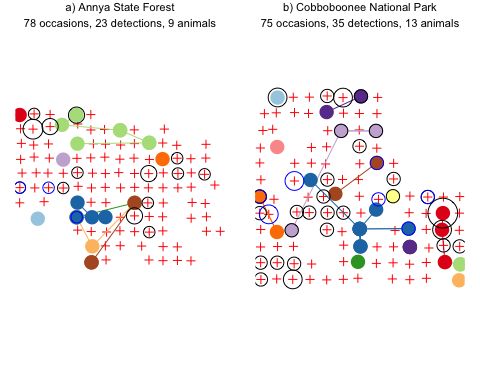
\includegraphics[width=1\linewidth]{figure/density-plot-ch-1-1} 

}

\caption{Feral cat detections in the first replicate grid pair in the Glenelg region, Australia. Camera-traps are indicated by red crosses. Solid fill coloured circles represent identified cats with lines indicating observed movements. Black open circles indicate black cat detections; blue circles indicate unidentifiable tabby cat detections, with circle radius scaling positively with the number of daily detections. Fox control does not occur in Annya (a) but does in Cobboboonee (b).}\label{fig:density-plot-ch-1}
\end{figure}
\newpage

\hypertarget{replicate-2}{%
\subsubsection{Replicate 2}\label{replicate-2}}

\(~\)

\(~\)

\(~\)
\begin{figure}

{\centering 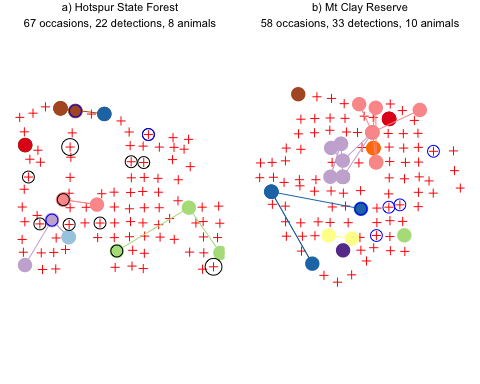
\includegraphics[width=1\linewidth]{figure/density-plot-ch-2-1} 

}

\caption{Feral cat detections in the second replicate grid pair in the Glenelg region, Australia. Camera-traps are indicated by red crosses. Solid fill coloured circles represent identified cats with lines indicating observed movements. Black open circles indicate black cat detections; blue circles indicate unidentifiable tabby cat detections, with circle radius scaling positively with the number of daily detections. Fox control does not occur in Hotspur (a) but does in Mt Clay (b).}\label{fig:density-plot-ch-2}
\end{figure}
\newpage

\hypertarget{replicate-3}{%
\subsubsection{Replicate 3}\label{replicate-3}}

\(~\)

\(~\)

\(~\)
\begin{figure}

{\centering 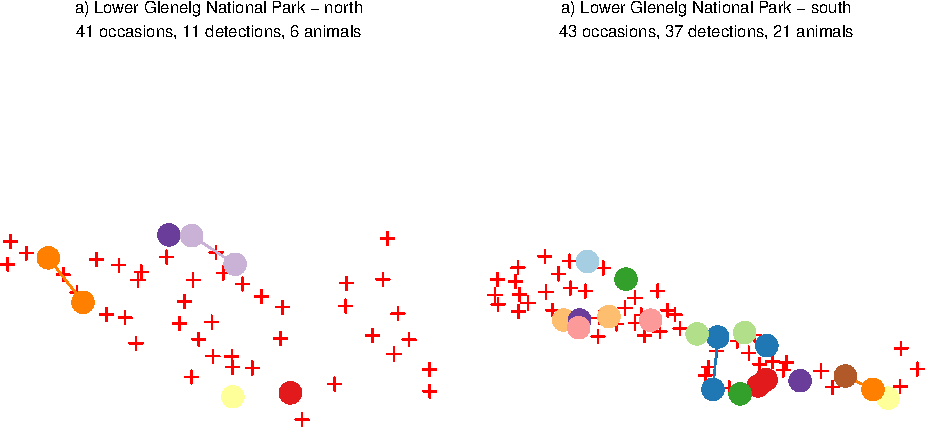
\includegraphics[width=1\linewidth]{figure/density-plot-ch-3-1} 

}

\caption{Feral cat detections in the third replicate grid pair in the Glenelg region, Australia. Camera-traps are indicated by red crosses. Solid fill coloured circles represent identified cats with lines indicating observed movements. Fox control does not occur in the north (a) but does in the south (b).}\label{fig:density-plot-ch-3}
\end{figure}
\newpage

\hypertarget{otway-region}{%
\subsection{Otway region}\label{otway-region}}

\hypertarget{section}{%
\subsubsection{2017}\label{section}}

\(~\)

\(~\)

\(~\)
\begin{figure}

{\centering 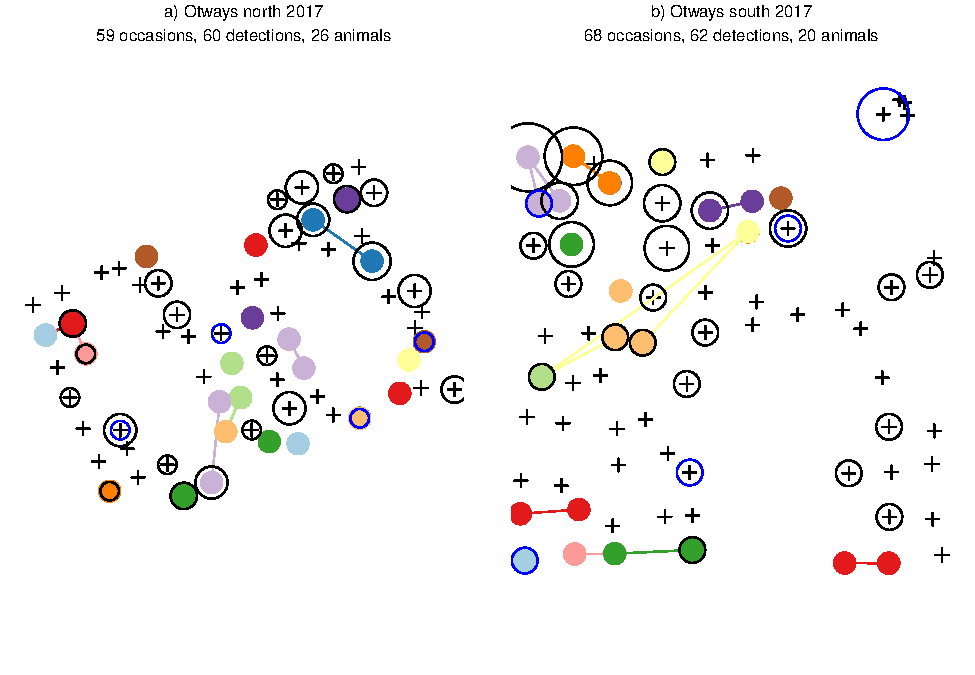
\includegraphics[width=1\linewidth]{figure/density-plot-ch-4-1} 

}

\caption{Feral cat detections in the Otway region, Australia, 2017. Solid fill coloured circles represent identified cats with lines indicating observed movements. Black open circles indicate black cat detections; blue circles indicate unidentifiable tabby cat detections, with circle radius scaling positively with the number of daily detections. Fox control did not occur in either of the landscapes during this time.}\label{fig:density-plot-ch-4}
\end{figure}
\newpage

\hypertarget{section-1}{%
\subsubsection{2018}\label{section-1}}

\(~\)

\(~\)

\(~\)
\begin{figure}

{\centering 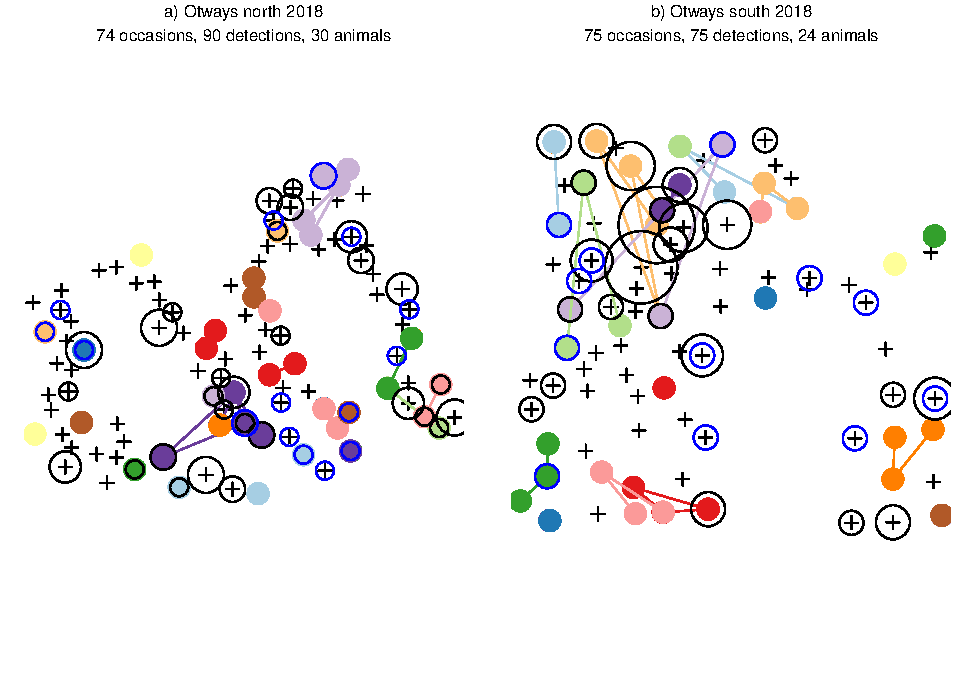
\includegraphics[width=1\linewidth]{figure/density-plot-ch-5-1} 

}

\caption{Feral cat detections in the Otway region, Australia, 2018. Solid fill coloured circles represent identified cats with lines indicating observed movements. Black open circles indicate black cat detections; blue circles indicate unidentifiable tabby cat detections, with circle radius scaling positively with the number of daily detections. Fox control had occurred, but lapsed just prior to the survey in the northern landscape (a), and did not occur in the southern landscape (b).}\label{fig:density-plot-ch-5}
\end{figure}
\newpage

\hypertarget{section-2}{%
\subsubsection{2019}\label{section-2}}

\(~\)

\(~\)

\(~\)
\begin{figure}

{\centering 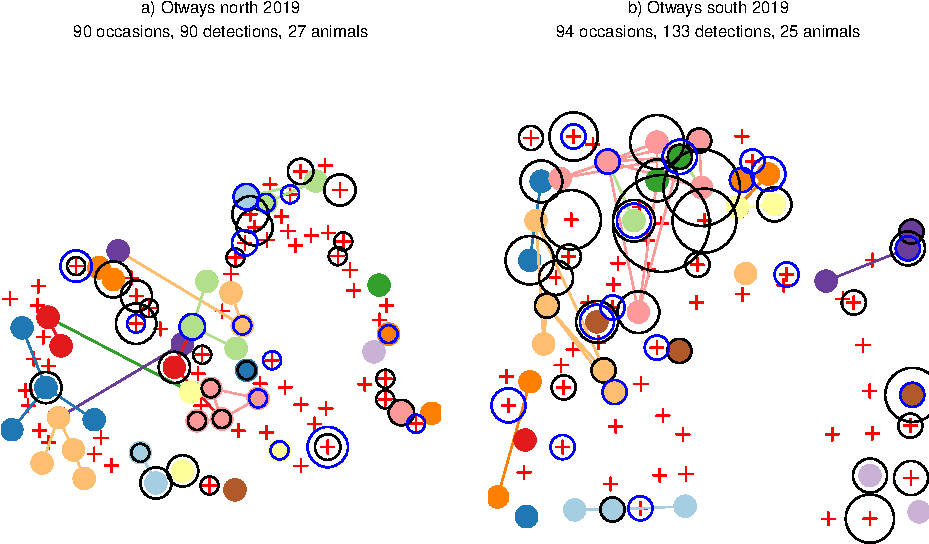
\includegraphics[width=1\linewidth]{figure/density-plot-ch-6-1} 

}

\caption{Feral cat detections in the Otway region, Australia, 2019. Solid fill coloured circles represent identified cats with lines indicating observed movements. Black open circles indicate black cat detections; blue circles indicate unidentifiable tabby cat detections, with circle radius scaling positively with the number of daily detections. Fox control occurred in the northern landscape (a) during this survey, but not the southern landscape (b).}\label{fig:density-plot-ch-6}
\end{figure}
\newpage

\hypertarget{density-app-fox}{%
\section{Fox spatial occurrence}\label{density-app-fox}}

\hypertarget{glenelg-region-4}{%
\subsection{Glenelg region}\label{glenelg-region-4}}

\(~\)

\(~\)

\(~\)
\begin{verbatim}
Family: binomial 
Link function: logit 

Formula:
fox ~ s(x, y, bs = "ds", m = c(1, 0.5), k = 200) + offset(log(survey_duration))

Parametric coefficients:
            Estimate Std. Error z value Pr(>|z|)    
(Intercept) -4.53965    0.09293  -48.85   <2e-16 ***
---
Signif. codes:  0 '***' 0.001 '**' 0.01 '*' 0.05 '.' 0.1 ' ' 1

Approximate significance of smooth terms:
         edf Ref.df Chi.sq  p-value    
s(x,y) 25.58    199  61.78 9.75e-07 ***
---
Signif. codes:  0 '***' 0.001 '**' 0.01 '*' 0.05 '.' 0.1 ' ' 1

R-sq.(adj) =  0.126   Deviance explained = 13.1%
fREML = 845.52  Scale est. = 1         n = 538
\end{verbatim}
\newpage

\(~\)

\(~\)

\(~\)
\begin{figure}

{\centering 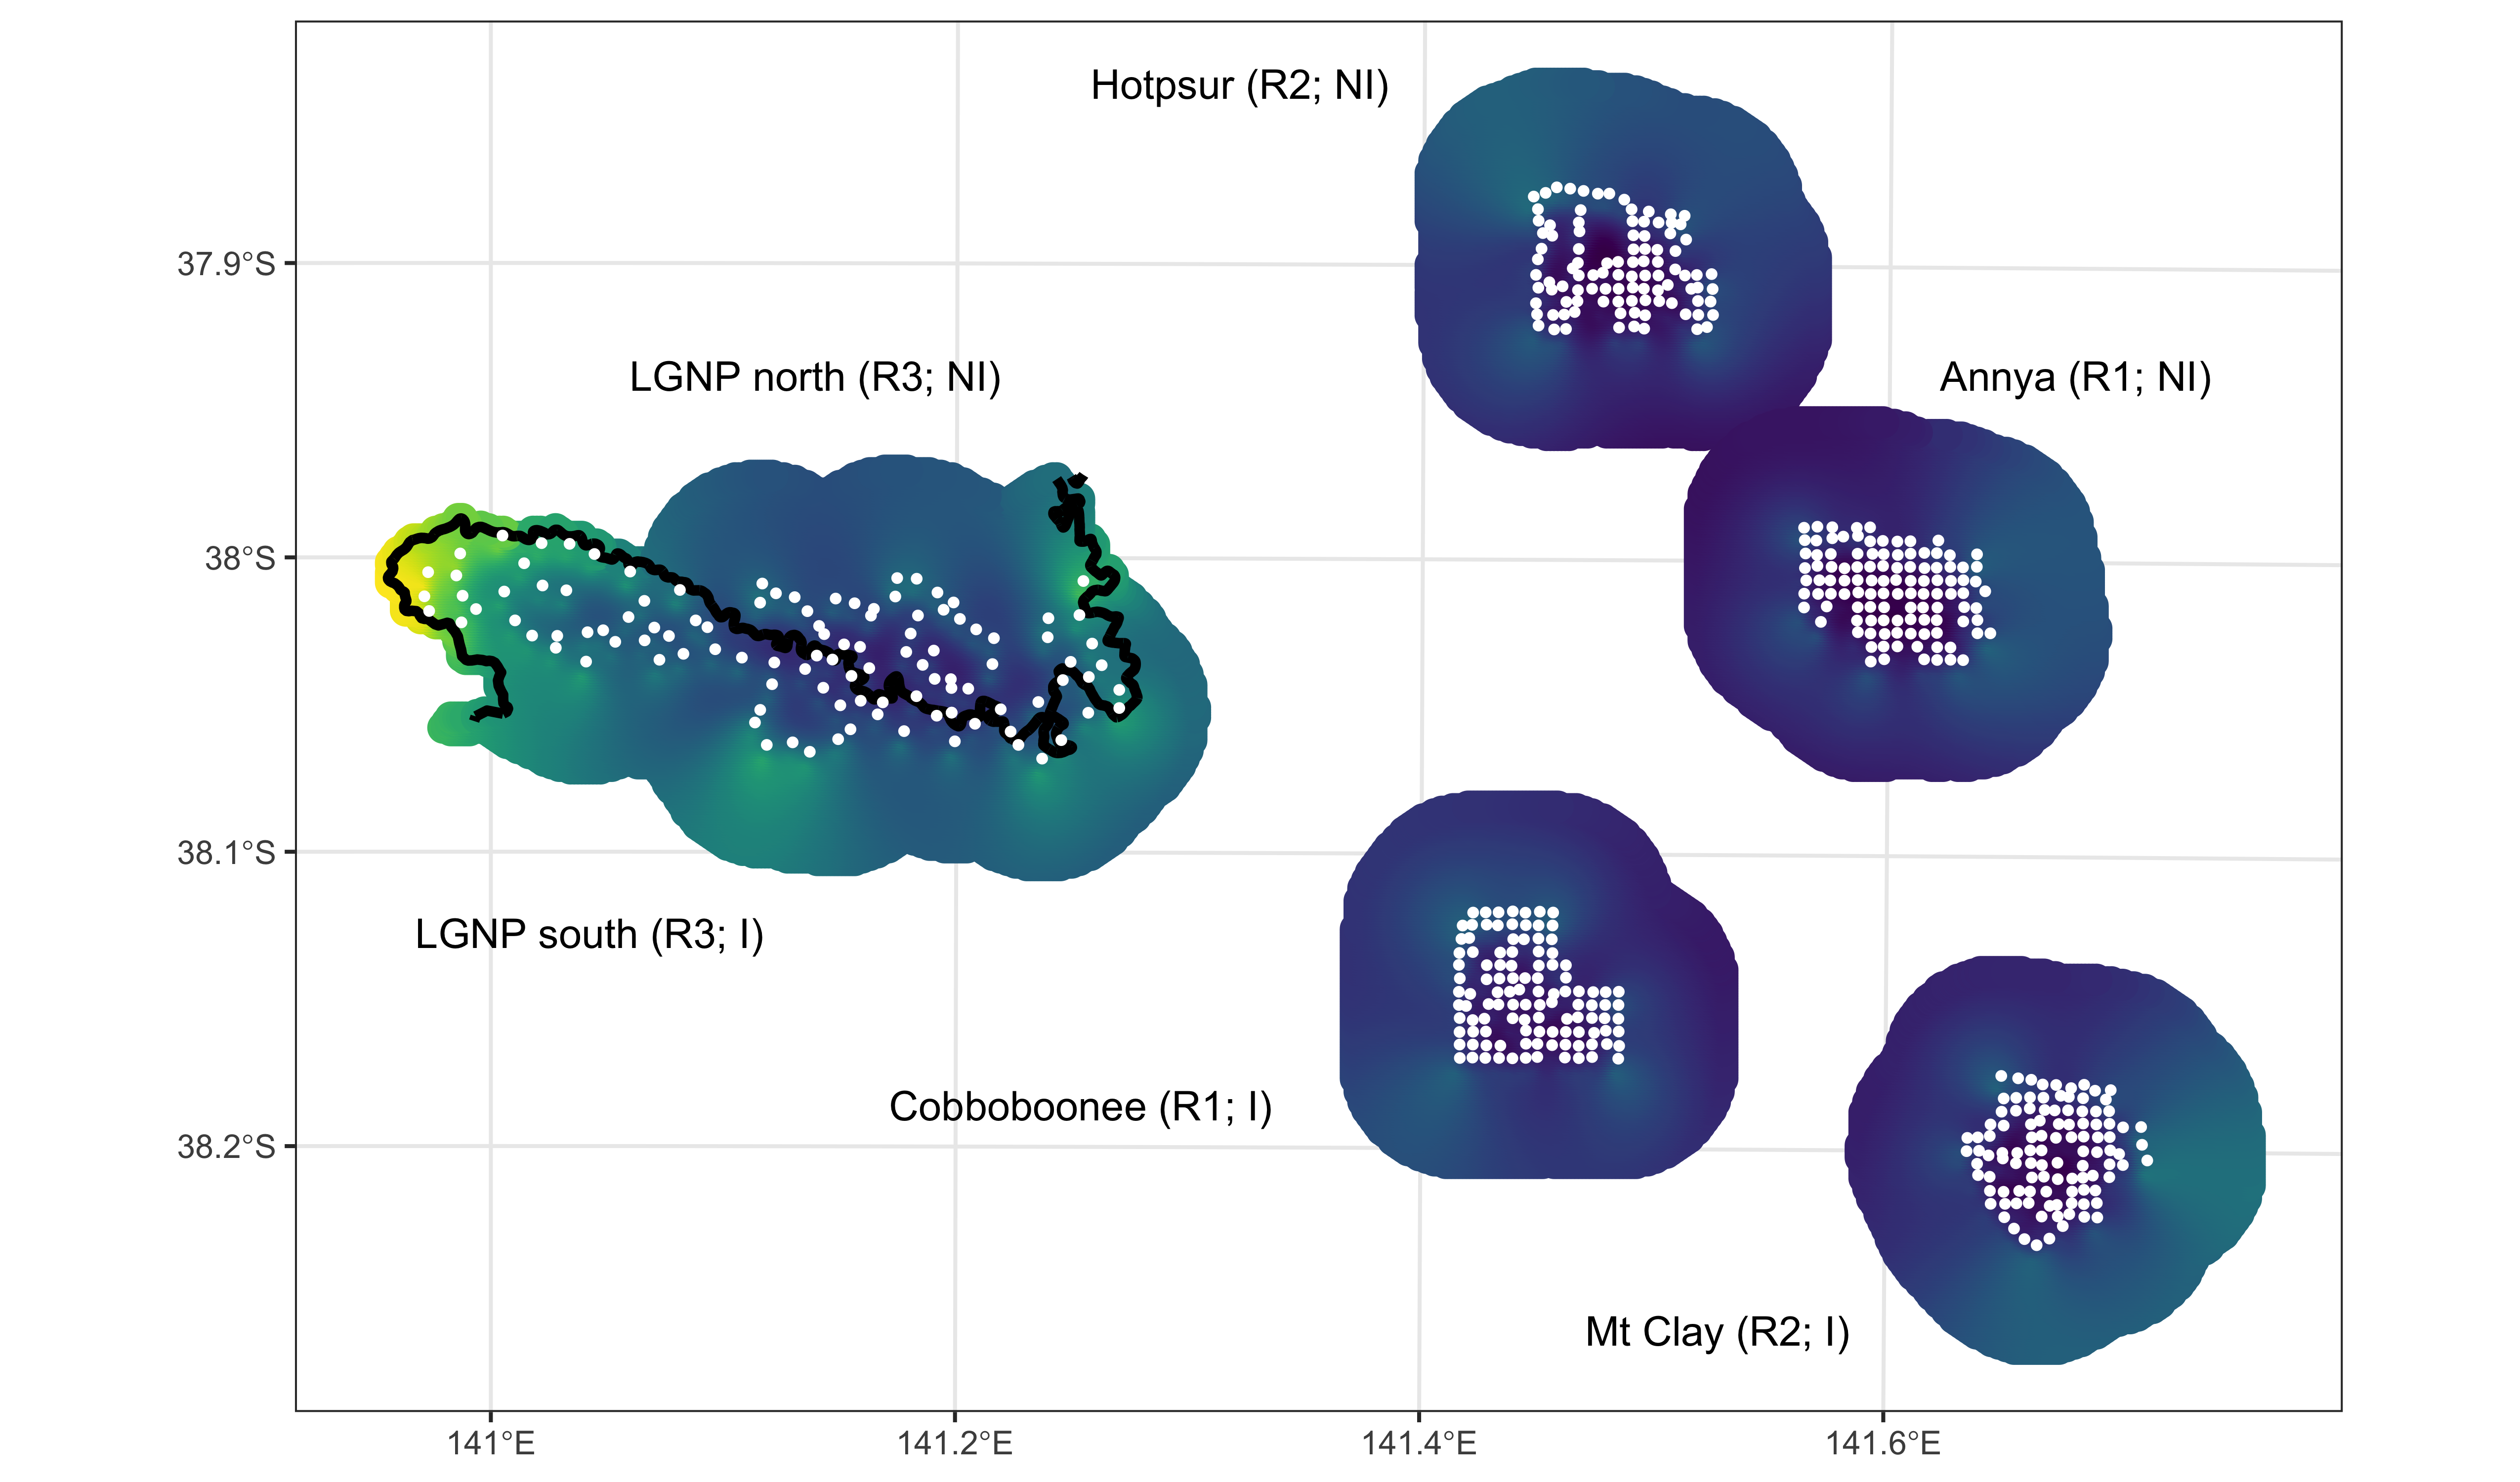
\includegraphics[width=1\linewidth]{figure/fox_occ_se_glenelg_600dpi} 

}

\caption{Standard error estimate of log fox occurrence probability derived from generalised additive models within each impact (I) and associated non-impact (NI) landscape in the Glenelg region, Australia.}\label{fig:density-fox-se-g}
\end{figure}
\newpage

\hypertarget{otway-region-1}{%
\subsection{Otway Region}\label{otway-region-1}}

\(~\)

\(~\)

\(~\)
\begin{verbatim}
Family: binomial 
Link function: logit 

Formula:
fox ~ year + s(x, y, by = year, bs = "ds", m = c(1, 0.5), k = 100) + 
    s(station, bs = "re") + offset(log(survey_duration))

Parametric coefficients:
             Estimate Std. Error z value Pr(>|z|)    
(Intercept) -5.283154   0.230023 -22.968   <2e-16 ***
year2018     0.004643   0.277696   0.017    0.987    
year2019     0.037119   0.282270   0.132    0.895    
---
Signif. codes:  0 '***' 0.001 '**' 0.01 '*' 0.05 '.' 0.1 ' ' 1

Approximate significance of smooth terms:
                      edf Ref.df Chi.sq  p-value    
s(x,y):year2017 2.688e+00     99  8.096 0.010597 *  
s(x,y):year2018 2.494e-05     99  0.000 0.506341    
s(x,y):year2019 6.148e+00     99 22.262 0.000380 ***
s(station)      5.366e+01    194 75.723 0.000116 ***
---
Signif. codes:  0 '***' 0.001 '**' 0.01 '*' 0.05 '.' 0.1 ' ' 1

R-sq.(adj) =   0.24   Deviance explained = 27.8%
fREML = 763.36  Scale est. = 1         n = 513
\end{verbatim}
\newpage

\(~\)

\(~\)

\(~\)
\begin{figure}

{\centering 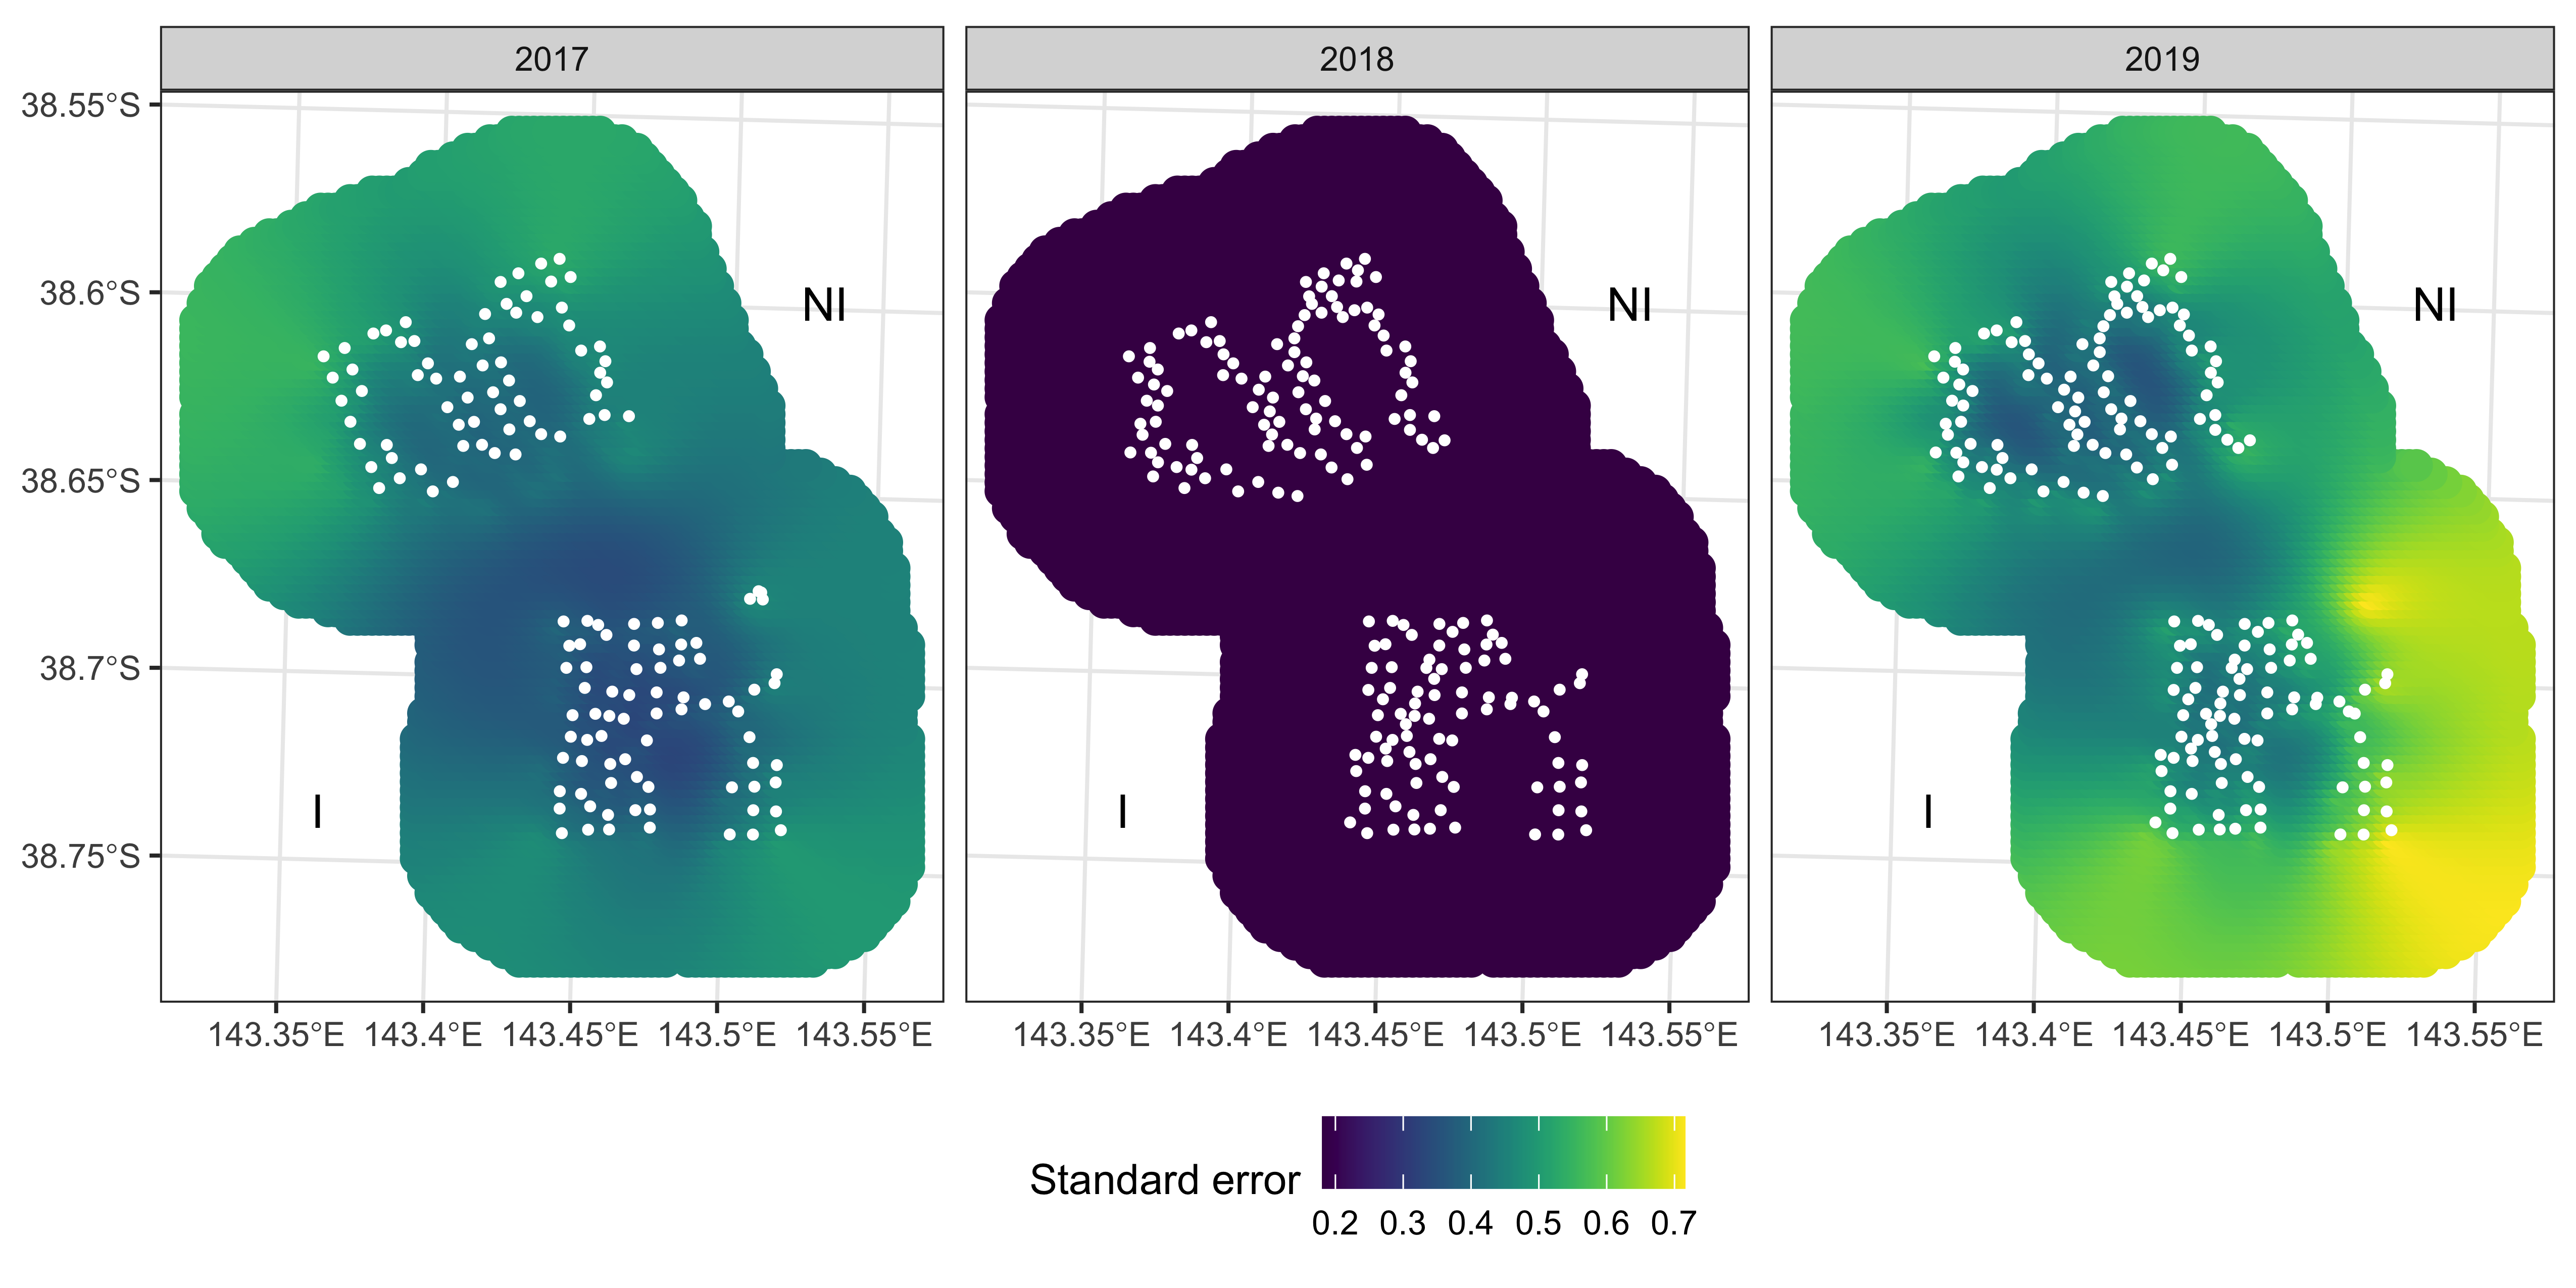
\includegraphics[width=1\linewidth]{figure/fox_occ_se_otways_600dpi} 

}

\caption{Standard error estimate of log fox occurrence probability derived from generalised additive models within each impact (I) and associated non-impact (NI) landscape in the Otway region, Australia.}\label{fig:density-fox-se-o}
\end{figure}
\newpage

\hypertarget{density-app-veg}{%
\section{Vegetation categories}\label{density-app-veg}}

We condensed the main Ecological Vegetation Class groupings (Department of Environment, Land, Water \& Planning 2020a) present into three categories for each region: cleared land, heathy woodlands, lowland forests (Glenelg region only) and wet forests (Otways region only). We merged similar groups to reduce the number of categories for each region. In the Glenelg region, we merged dry forests with lowland forests. In the Otway region, we merged rainforests with wet forests, as well as merged dry forests and heathy woodlands.

A very small proportion of other Ecological Vegetation Class groupings were present in the habitat masks: riparian scrubs or swampy scrubs and woodlands, coastal scrubs grasslands and woodlands, wetlands, riverine grassy woodlands or forests, plains woodlands or forests, herb-rich woodlands. We removed these groups, and interpolated cell values from the nearest of the three vegetation categories.

\newpage

\(~\)

\(~\)

\(~\)
\begin{figure}

{\centering 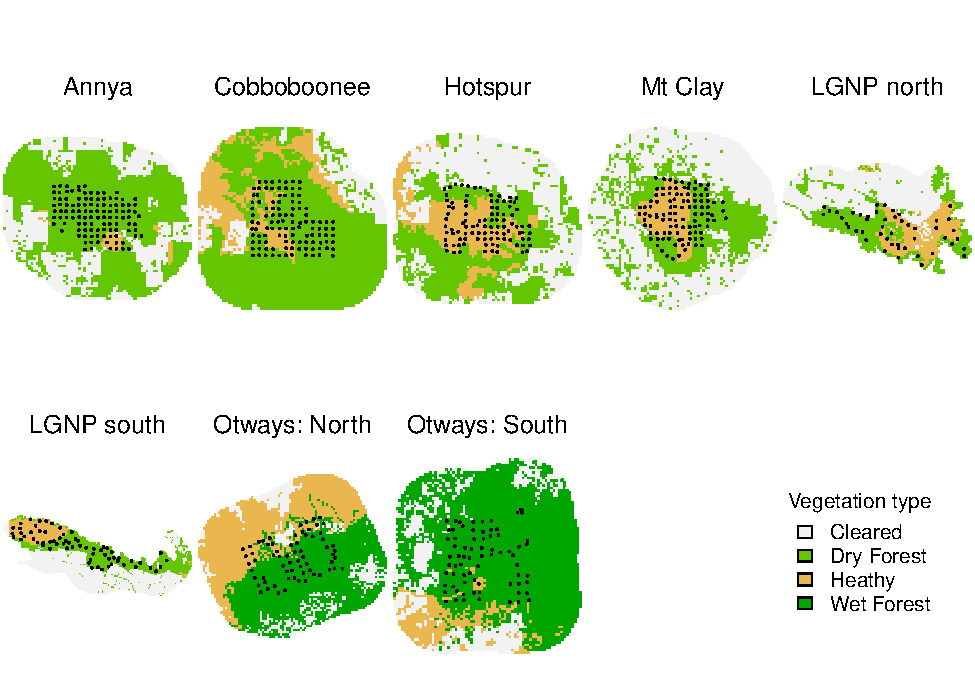
\includegraphics[width=1\linewidth]{figure/density-veg-1} 

}

\caption{Condensed Ecological Vegetation Class groups used as habitat mask covariates in spatial mark-resight models.}\label{fig:density-veg}
\end{figure}
\newpage

\hypertarget{spatial-mark-resight-models}{%
\section{Spatial mark-resight models}\label{spatial-mark-resight-models}}

\hypertarget{glenelg-region-5}{%
\subsection{Glenelg region}\label{glenelg-region-5}}

\(~\)

\(~\)

\(~\)

\begingroup\fontsize{10}{12}\selectfont
\begin{longtable}[t]{lrrrrrr}
\caption{\label{tab:density-aic-g-1}Akaike's Information Criterion values adjusted for small sample size for feral cat density models in the Glenelg region; model set 1.}\\
\toprule
Detector function & K & logLik & AIC & AICc & dAICc & AICcwt\\
\midrule
exponential & 3 & -1745.99 & 3497.99 & 3498.37 & 0.00 & 1\\
half-normal & 3 & -1763.02 & 3532.04 & 3532.43 & 34.06 & 0\\
\bottomrule
\multicolumn{7}{l}{\rule{0pt}{1em}K - number of parameters}\\
\multicolumn{7}{l}{\rule{0pt}{1em}AICc - Akaike's Information Criterion with small-sample adjustment}\\
\multicolumn{7}{l}{\rule{0pt}{1em}dAICc - difference between AICc of this model and the model with smallest AICc}\\
\multicolumn{7}{l}{\rule{0pt}{1em}AICcwt - AICc model weight}\\
\end{longtable}
\endgroup{}

\newpage

\(~\)

\(~\)

\(~\)

\begingroup\fontsize{10}{12}\selectfont
\begin{longtable}[t]{lrrrrrr}
\caption{\label{tab:density-aic-g-2}Akaike's Information Criterion values adjusted for small sample size for feral cat density models in the Glenelg region; model set 2.}\\
\toprule
Model & K & logLik & AIC & AICc & dAICc & AICcwt\\
\midrule
D\textasciitilde{}1 g0\textasciitilde{}1 sigma\textasciitilde{}1 & 3 & -1309.93 & 2625.85 & 2626.23 & 0.00 & 0.32\\
D\textasciitilde{}vegetation g0\textasciitilde{}1 sigma\textasciitilde{}1 & 5 & -1307.68 & 2625.37 & 2626.35 & 0.12 & 0.30\\
D\textasciitilde{}vegetation g0\textasciitilde{}T sigma\textasciitilde{}1 & 6 & -1306.89 & 2625.77 & 2627.17 & 0.94 & 0.20\\
D\textasciitilde{}1 g0\textasciitilde{}T sigma\textasciitilde{}1 & 4 & -1309.32 & 2626.65 & 2627.29 & 1.06 & 0.19\\
\bottomrule
\multicolumn{7}{l}{\rule{0pt}{1em}K - number of parameters}\\
\multicolumn{7}{l}{\rule{0pt}{1em}AICc - Akaike's Information Criterion with small-sample adjustment}\\
\multicolumn{7}{l}{\rule{0pt}{1em}dAICc - difference between AICc of this model and the model with smallest AICc}\\
\multicolumn{7}{l}{\rule{0pt}{1em}AICcwt - AICc model weight}\\
\multicolumn{7}{l}{\rule{0pt}{1em}T - linear time trend (g0 only)}\\
\end{longtable}
\endgroup{}

\newpage

\(~\)

\(~\)

\(~\)

\begingroup\fontsize{10}{12}\selectfont
\begin{longtable}[t]{lrrrrrr}
\caption{\label{tab:density-aic-g-3}Akaike's Information Criterion values adjusted for small sample size for feral cat density models in the Glenelg region; model set 3.}\\
\toprule
Model & K & logLik & AIC & AICc & dAICc & AICcwt\\
\midrule
D\textasciitilde{}fox\_occ g0\textasciitilde{}1 sigma\textasciitilde{}1 & 4 & -1306.67 & 2621.33 & 2621.98 & 0.00 & 0.49\\
D\textasciitilde{}fox\_occ g0\textasciitilde{}fox\_occ sigma\textasciitilde{}fox\_occ & 6 & -1304.97 & 2621.94 & 2623.34 & 1.36 & 0.25\\
D\textasciitilde{}s(fox\_occ) g0\textasciitilde{}1 sigma\textasciitilde{}1 & 5 & -1306.61 & 2623.21 & 2624.20 & 2.22 & 0.16\\
D\textasciitilde{}1 g0\textasciitilde{}1 sigma\textasciitilde{}1 & 3 & -1309.93 & 2625.85 & 2626.23 & 4.26 & 0.06\\
D\textasciitilde{}s(fox\_occ) g0\textasciitilde{}s(fox\_occ) sigma\textasciitilde{}s(fox\_occ) & 9 & -1303.41 & 2624.81 & 2627.97 & 5.99 & 0.02\\
\addlinespace
D\textasciitilde{}1 g0\textasciitilde{}fox\_occ sigma\textasciitilde{}fox\_occ & 5 & -1309.41 & 2628.82 & 2629.80 & 7.82 & 0.01\\
D\textasciitilde{}1 g0\textasciitilde{}s(fox\_occ) sigma\textasciitilde{}s(fox\_occ) & 7 & -1307.91 & 2629.81 & 2631.71 & 9.73 & 0.00\\
\bottomrule
\multicolumn{7}{l}{\rule{0pt}{1em}K - number of parameters}\\
\multicolumn{7}{l}{\rule{0pt}{1em}AICc - Akaike's Information Criterion with small-sample adjustment}\\
\multicolumn{7}{l}{\rule{0pt}{1em}dAICc - difference between AICc of this model and the model with smallest AICc}\\
\multicolumn{7}{l}{\rule{0pt}{1em}AICcwt - AICc model weight}\\
\multicolumn{7}{l}{\rule{0pt}{1em}fox\_occ - fine-scale occurrence probability of foxes derived from generalised additive models}\\
\multicolumn{7}{l}{\rule{0pt}{1em}s(fox\_occ) - non-linear smooth of fox\_occ with three knots}\\
\end{longtable}
\endgroup{}

\newpage

\(~\)

\(~\)

\(~\)

\begingroup\fontsize{10}{12}\selectfont
\begin{longtable}[t]{lrrrrrr}
\caption{\label{tab:density-aic-g-4}Akaike's Information Criterion values adjusted for small sample size for feral cat density models in the Glenelg region; model set 4.}\\
\toprule
Model & K & logLik & AIC & AICc & dAICc & AICcwt\\
\midrule
D\textasciitilde{}session g0\textasciitilde{}fox\_occ sigma\textasciitilde{}fox\_occ & 10 & -1297.46 & 2614.93 & 2618.86 & 0.00 & 0.62\\
D\textasciitilde{}session g0\textasciitilde{}1 sigma\textasciitilde{}1 & 8 & -1300.66 & 2617.32 & 2619.80 & 0.95 & 0.38\\
\bottomrule
\multicolumn{7}{l}{\rule{0pt}{1em}K - number of parameters}\\
\multicolumn{7}{l}{\rule{0pt}{1em}AICc - Akaike's Information Criterion with small-sample adjustment}\\
\multicolumn{7}{l}{\rule{0pt}{1em}dAICc - difference between AICc of this model and the model with smallest AICc}\\
\multicolumn{7}{l}{\rule{0pt}{1em}AICcwt - AICc model weight}\\
\multicolumn{7}{l}{\rule{0pt}{1em}fox\_occ - fine-scale occurrence probability of foxes derived from generalised additive models}\\
\multicolumn{7}{l}{\rule{0pt}{1em}session - landscape (n = 6)}\\
\end{longtable}
\endgroup{}

\newpage

\(~\)

\(~\)

\(~\)

\begingroup\fontsize{10}{12}\selectfont
\begin{longtable}[t]{lrrrll}
\caption{\label{tab:density-landscape-est}Feral cat density per square kilometre as estimated by the AICc top-ranked model in the Glenelg region, Australia.}\\
\toprule
Landscape & Estimate & 5\% CI & 95\% CI & Treatment & Replicate\\
\midrule
Annya & 0.24 & 0.17 & 0.34 & Non-impact & 1\\
Cobboboonee & 0.60 & 0.40 & 0.88 & Impact & 1\\
Hotspur & 0.22 & 0.14 & 0.33 & Non-impact & 2\\
Mt Clay & 0.24 & 0.18 & 0.31 & Impact & 2\\
LGNP north & 0.15 & 0.07 & 0.35 & Non-impact & 3\\
\addlinespace
LGNP south & 0.56 & 0.34 & 0.90 & Impact & 3\\
\bottomrule
\end{longtable}
\endgroup{}

\newpage

\hypertarget{otway-region-2}{%
\subsection{Otway region}\label{otway-region-2}}

\(~\)

\(~\)

\(~\)

\begingroup\fontsize{10}{12}\selectfont
\begin{longtable}[t]{lrrrrrr}
\caption{\label{tab:density-aic-o-1}Akaike's Information Criterion values for detector functions in the Otway region, Australia; model set 1.}\\
\toprule
Detector function & K & logLik & AIC & AICc & dAICc & AICcwt\\
\midrule
exponential & 3 & -5591.00 & 11188.01 & 11188.17 & 0.00 & 1\\
half-normal & 3 & -5743.26 & 11492.52 & 11492.69 & 304.52 & 0\\
\bottomrule
\multicolumn{7}{l}{\rule{0pt}{1em}K - number of parameters}\\
\multicolumn{7}{l}{\rule{0pt}{1em}AICc - Akaike's Information Criterion with small-sample adjustment}\\
\multicolumn{7}{l}{\rule{0pt}{1em}dAICc - difference between AICc of this model and the model with smallest AICc}\\
\multicolumn{7}{l}{\rule{0pt}{1em}AICcwt - AICc model weight}\\
\end{longtable}
\endgroup{}

\newpage

\(~\)

\(~\)

\(~\)

\begingroup\fontsize{10}{12}\selectfont
\begin{longtable}[t]{lrrrrrr}
\caption{\label{tab:density-aic-o-2}Akaike's Information Criterion values adjusted for small sample size for feral cat density models in the Otway region; model set 2.}\\
\toprule
Model & K & logLik & AIC & AICc & dAICc & AICcwt\\
\midrule
D\textasciitilde{}year g0\textasciitilde{}1 sigma\textasciitilde{}1 & 5 & -3550.63 & 7111.26 & 7111.67 & 0.00 & 0.48\\
D\textasciitilde{}year g0\textasciitilde{}T sigma\textasciitilde{}1 & 6 & -3549.83 & 7111.67 & 7112.25 & 0.57 & 0.36\\
D\textasciitilde{}year + vegetation g0\textasciitilde{}1 sigma\textasciitilde{}1 & 7 & -3550.04 & 7114.08 & 7114.86 & 3.19 & 0.10\\
D\textasciitilde{}year + vegetation g0\textasciitilde{}T sigma\textasciitilde{}1 & 8 & -3549.24 & 7114.48 & 7115.49 & 3.82 & 0.07\\
\bottomrule
\multicolumn{7}{l}{\rule{0pt}{1em}K - number of parameters}\\
\multicolumn{7}{l}{\rule{0pt}{1em}AICc - Akaike's Information Criterion with small-sample adjustment}\\
\multicolumn{7}{l}{\rule{0pt}{1em}dAICc - difference between AICc of this model and the model with smallest AICc}\\
\multicolumn{7}{l}{\rule{0pt}{1em}AICcwt - AICc model weight}\\
\multicolumn{7}{l}{\rule{0pt}{1em}T - linear time trend (g0 only)}\\
\end{longtable}
\endgroup{}

\newpage

\(~\)

\(~\)

\(~\)

\begingroup\fontsize{10}{12}\selectfont
\begin{longtable}[t]{lrrrrrr}
\caption{\label{tab:density-aic-o-3}Akaike's Information Criterion values adjusted for small sample size for feral cat density models in the Otway region; model set 3.}\\
\toprule
Model & K & logLik & AIC & AICc & dAICc & AICcwt\\
\midrule
D\textasciitilde{}year + fox\_occ g0\textasciitilde{}fox\_occ sigma\textasciitilde{}fox\_occ & 8 & -3541.80 & 7099.59 & 7100.60 & 0.00 & 0.33\\
D\textasciitilde{}year + s(fox\_occ) g0\textasciitilde{}s(fox\_occ) sigma\textasciitilde{}s(fox\_occ) & 11 & -3538.59 & 7099.19 & 7101.07 & 0.47 & 0.26\\
D\textasciitilde{}year g0\textasciitilde{}s(fox\_occ) sigma\textasciitilde{}s(fox\_occ) & 9 & -3541.07 & 7100.13 & 7101.40 & 0.80 & 0.22\\
D\textasciitilde{}year g0\textasciitilde{}fox\_occ sigma\textasciitilde{}fox\_occ & 7 & -3543.44 & 7100.87 & 7101.65 & 1.05 & 0.19\\
D\textasciitilde{}year + fox\_occ g0\textasciitilde{}1 sigma\textasciitilde{}1 & 6 & -3548.26 & 7108.51 & 7109.09 & 8.49 & 0.00\\
\addlinespace
D\textasciitilde{}year + s(fox\_occ) g0\textasciitilde{}1 sigma\textasciitilde{}1 & 7 & -3547.47 & 7108.94 & 7109.72 & 9.12 & 0.00\\
D\textasciitilde{}year g0\textasciitilde{}1 sigma\textasciitilde{}1 & 5 & -3550.63 & 7111.26 & 7111.67 & 11.07 & 0.00\\
\bottomrule
\multicolumn{7}{l}{\rule{0pt}{1em}K - number of parameters}\\
\multicolumn{7}{l}{\rule{0pt}{1em}AICc - Akaike's Information Criterion with small-sample adjustment}\\
\multicolumn{7}{l}{\rule{0pt}{1em}dAICc - difference between AICc of this model and the model with smallest AICc}\\
\multicolumn{7}{l}{\rule{0pt}{1em}AICcwt - AICc model weight}\\
\multicolumn{7}{l}{\rule{0pt}{1em}fox\_occ - fine-scale occurrence probability of foxes derived from generalised additive models}\\
\multicolumn{7}{l}{\rule{0pt}{1em}s(fox\_occ) - non-linear smooth of fox\_occ with three knots}\\
\end{longtable}
\endgroup{}

\newpage

\(~\)

\(~\)

\(~\)

\begingroup\fontsize{10}{12}\selectfont
\begin{longtable}[t]{lrrrrrr}
\caption{\label{tab:density-aic-o-4}Akaike's Information Criterion values adjusted for small sample size for feral cat density models in the Otway region; model set 4.}\\
\toprule
Model & K & logLik & AIC & AICc & dAICc & AICcwt\\
\midrule
D\textasciitilde{}session g0\textasciitilde{}fox\_occ sigma\textasciitilde{}fox\_occ & 10 & -3541.77 & 7103.55 & 7105.11 & 0.00 & 0.99\\
D\textasciitilde{}session g0\textasciitilde{}1 sigma\textasciitilde{}1 & 8 & -3548.37 & 7112.73 & 7113.74 & 8.63 & 0.01\\
\bottomrule
\multicolumn{7}{l}{\rule{0pt}{1em}K - number of parameters}\\
\multicolumn{7}{l}{\rule{0pt}{1em}AICc - Akaike's Information Criterion with small-sample adjustment}\\
\multicolumn{7}{l}{\rule{0pt}{1em}dAICc - difference between AICc of this model and the model with smallest AICc}\\
\multicolumn{7}{l}{\rule{0pt}{1em}AICcwt - AICc model weight}\\
\multicolumn{7}{l}{\rule{0pt}{1em}fox\_occ - fine-scale occurrence probability of foxes derived from generalised additive models}\\
\multicolumn{7}{l}{\rule{0pt}{1em}session - landscape by year (n = 6)}\\
\end{longtable}
\endgroup{}

\newpage

\(~\)

\(~\)

\(~\)

\begingroup\fontsize{10}{12}\selectfont
\begin{longtable}[t]{lrrrll}
\caption{\label{tab:density-aic-o-5}Feral cat density per square kilometre as estimated by the AICc top-ranked model in the Otway region, Australia.}\\
\toprule
Landscape & Estimate & 5\% CI & 95\% CI & Treatment & Year\\
\midrule
north 2017 & 1.00 & 0.74 & 1.35 & Non-impact & 2017\\
south 2017 & 0.74 & 0.52 & 1.05 & Impact & 2017\\
north 2018 & 0.81 & 0.64 & 1.02 & Non-impact & 2018\\
south 2018 & 0.82 & 0.63 & 1.06 & Impact & 2018\\
north 2019 & 0.73 & 0.55 & 0.95 & Non-impact & 2019\\
\addlinespace
south 2019 & 0.98 & 0.76 & 1.27 & Impact & 2019\\
\bottomrule
\end{longtable}
\endgroup{}

\newpage

\hypertarget{diel-app}{%
\chapter{Supporting Information: Chapter \ref{diel}}\label{diel-app}}

\newpage

\(~\)

\(~\)

\(~\)

\begingroup\fontsize{10}{12}\selectfont
\begin{longtable}[t]{llrrrr}
\caption{\label{tab:diel-tab1}Summary of the number of camera-trap deployments, unique survey sites and 'independent' counts of invasive predator detections across Ecological Vegetation Class groups within the Glenelg and Otway regions, south-west Victoria, Australia.}\\
\toprule
Vegetation & Region & Sites & Deployments & Fox counts & Cat counts\\
\midrule
Dry Forest & Glenelg & 25 & 69 & 347 & 9\\
 & Otways & 111 & 314 & 341 & 158\\
Heathland & Glenelg & 40 & 119 & 265 & 59\\
 & Otways & 3 & 9 & 8 & 6\\
Heathy Woodland & Glenelg & 154 & 424 & 574 & 96\\
\addlinespace
 & Otways & 82 & 256 & 160 & 66\\
Herb-rich Woodland & Glenelg & 59 & 373 & 863 & 198\\
 & Otways & 2 & 6 & 3 & 2\\
Lowland Forest & Glenelg & 383 & 1046 & 1900 & 290\\
 & Otways & 52 & 163 & 190 & 35\\
\addlinespace
Swampy Scrub & Glenelg & 4 & 10 & 19 & 8\\
 & Otways & 36 & 98 & 64 & 88\\
Wet Forest & Otways & 281 & 780 & 715 & 1187\\
\textbf{Total} & \textbf{} & \textbf{1232} & \textbf{3667} & \textbf{5449} & \textbf{2202}\\
\bottomrule
\end{longtable}
\endgroup{}

\newpage

\begingroup\fontsize{10}{12}\selectfont
\begin{longtable}[t]{llrrr}
\caption{\label{tab:diel-tab-fits}Generalised additive model summaries for invasive predator spatiotemporal activity in south-west Victoria, Australia.}\\
\toprule
Species & Model & EDF & dev.expl & r.sq\\
\midrule
fox & 1\_spatial & 772.6469 & 0.3514 & 0.1170\\
fox & 2\_vegetation\_type & 766.1054 & 0.3498 & 0.1155\\
fox & 3\_habitat\_type & 768.2692 & 0.3487 & 0.1139\\
cat & 1\_spatial & 562.9236 & 0.2314 & 0.0772\\
cat & 2\_vegetation\_type & 566.7562 & 0.2300 & 0.0769\\
\addlinespace
cat & 3\_fox\_by\_habitat\_type & 585.8580 & 0.2317 & 0.0779\\
\bottomrule
\multicolumn{5}{l}{\rule{0pt}{1em}\textit{Note: }}\\
\multicolumn{5}{l}{\rule{0pt}{1em}EDF - estimated degrees of freedom of all model terms.}\\
\multicolumn{5}{l}{\rule{0pt}{1em}dev.expl - proportion of the null deviance explained by the model. }\\
\multicolumn{5}{l}{\rule{0pt}{1em}r.sq -  adjusted r-squared value.}\\
\end{longtable}
\endgroup{}

\newpage
\begin{figure}

{\centering 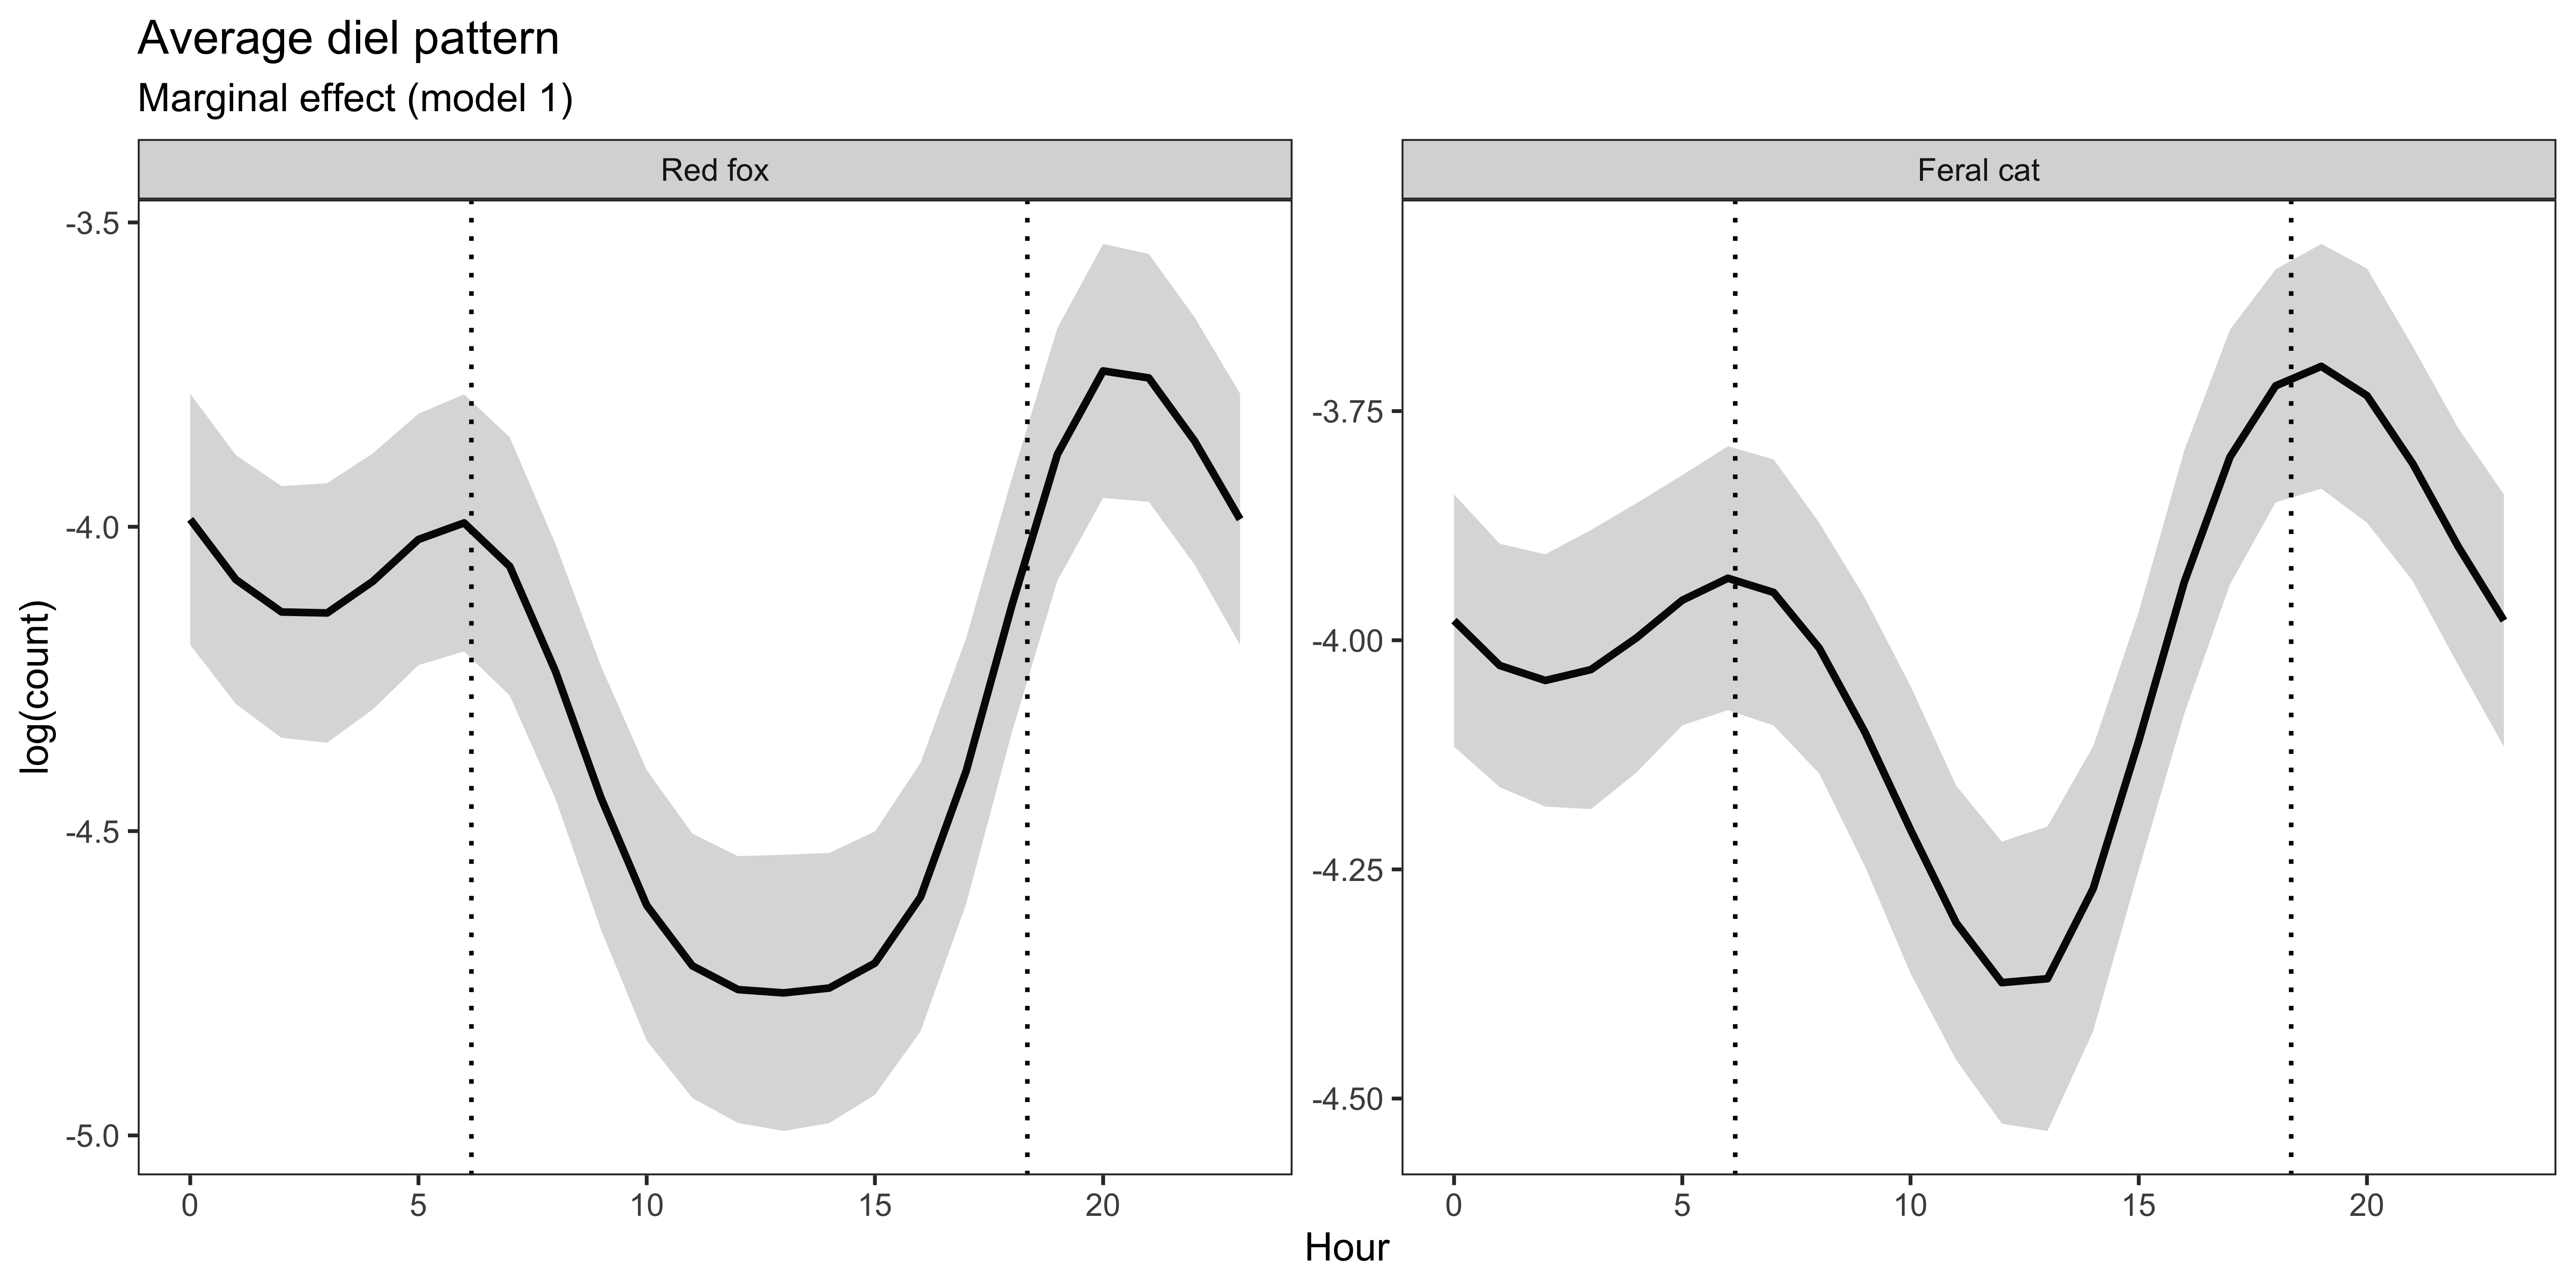
\includegraphics[width=1\linewidth]{figure/avg_diel_predator} 

}

\caption{Marginal effect of time (model 1) on predators across both study regions in south-west Victoria, Australia. White crosses depict unique camera-trap sites}\label{fig:diel-space-time-marginal}
\end{figure}
\newpage
\begin{center}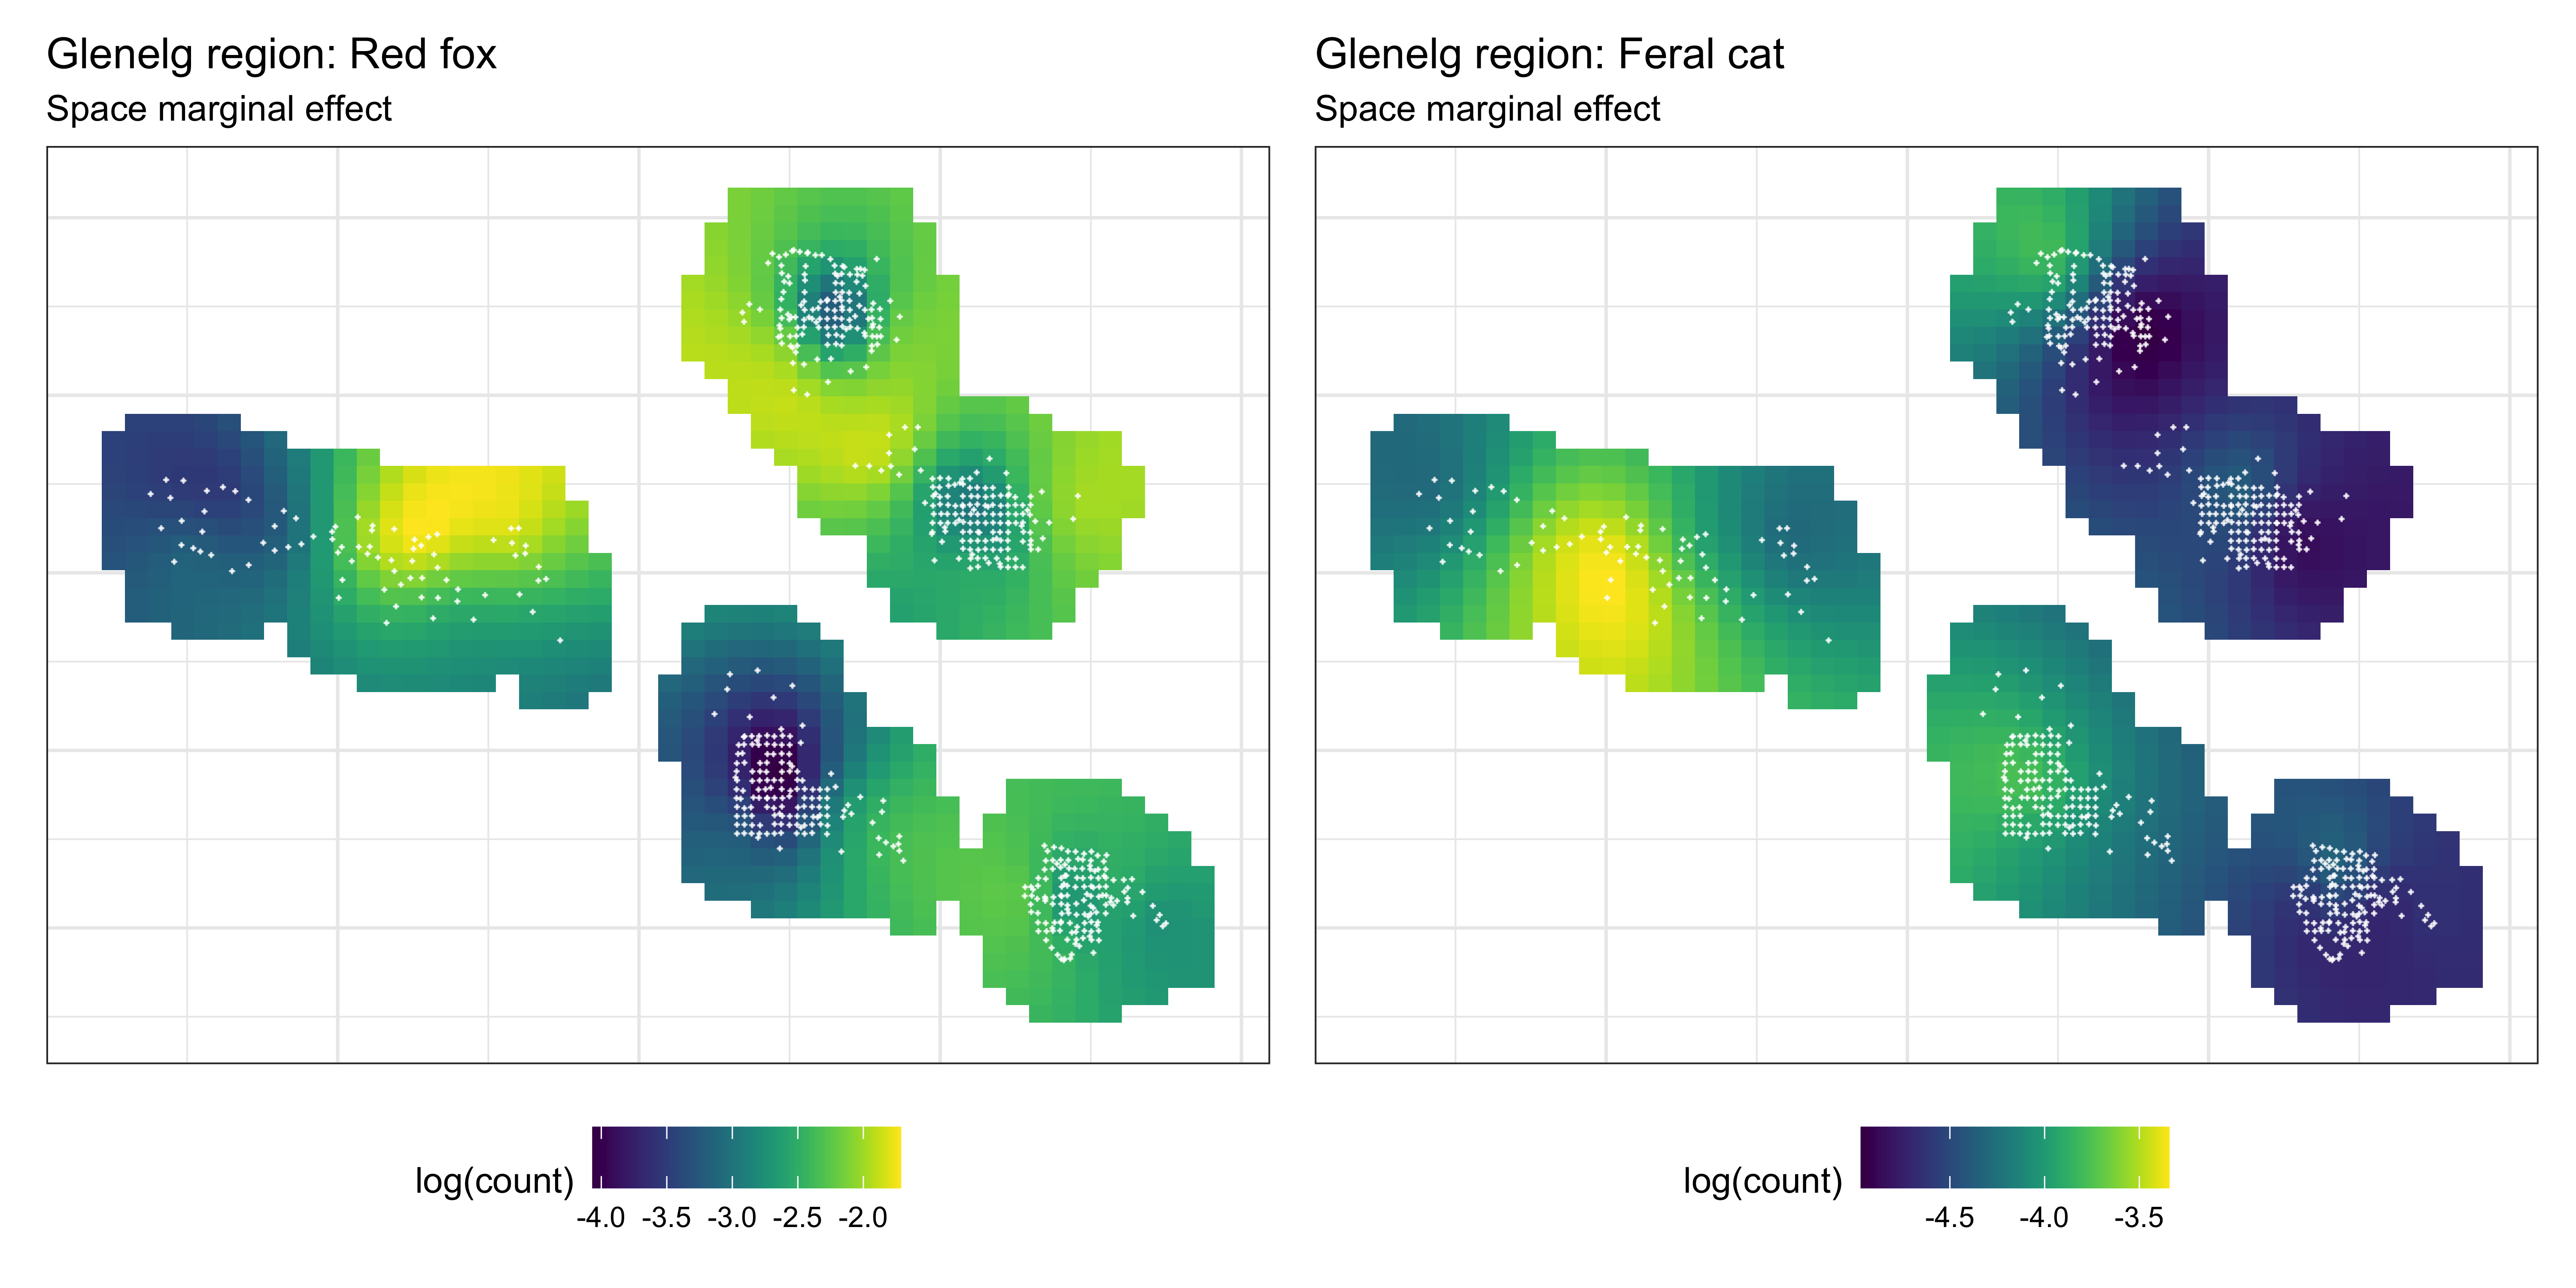
\includegraphics[width=1\linewidth]{figure/sp_marginal_g} \end{center}
\begin{figure}

{\centering 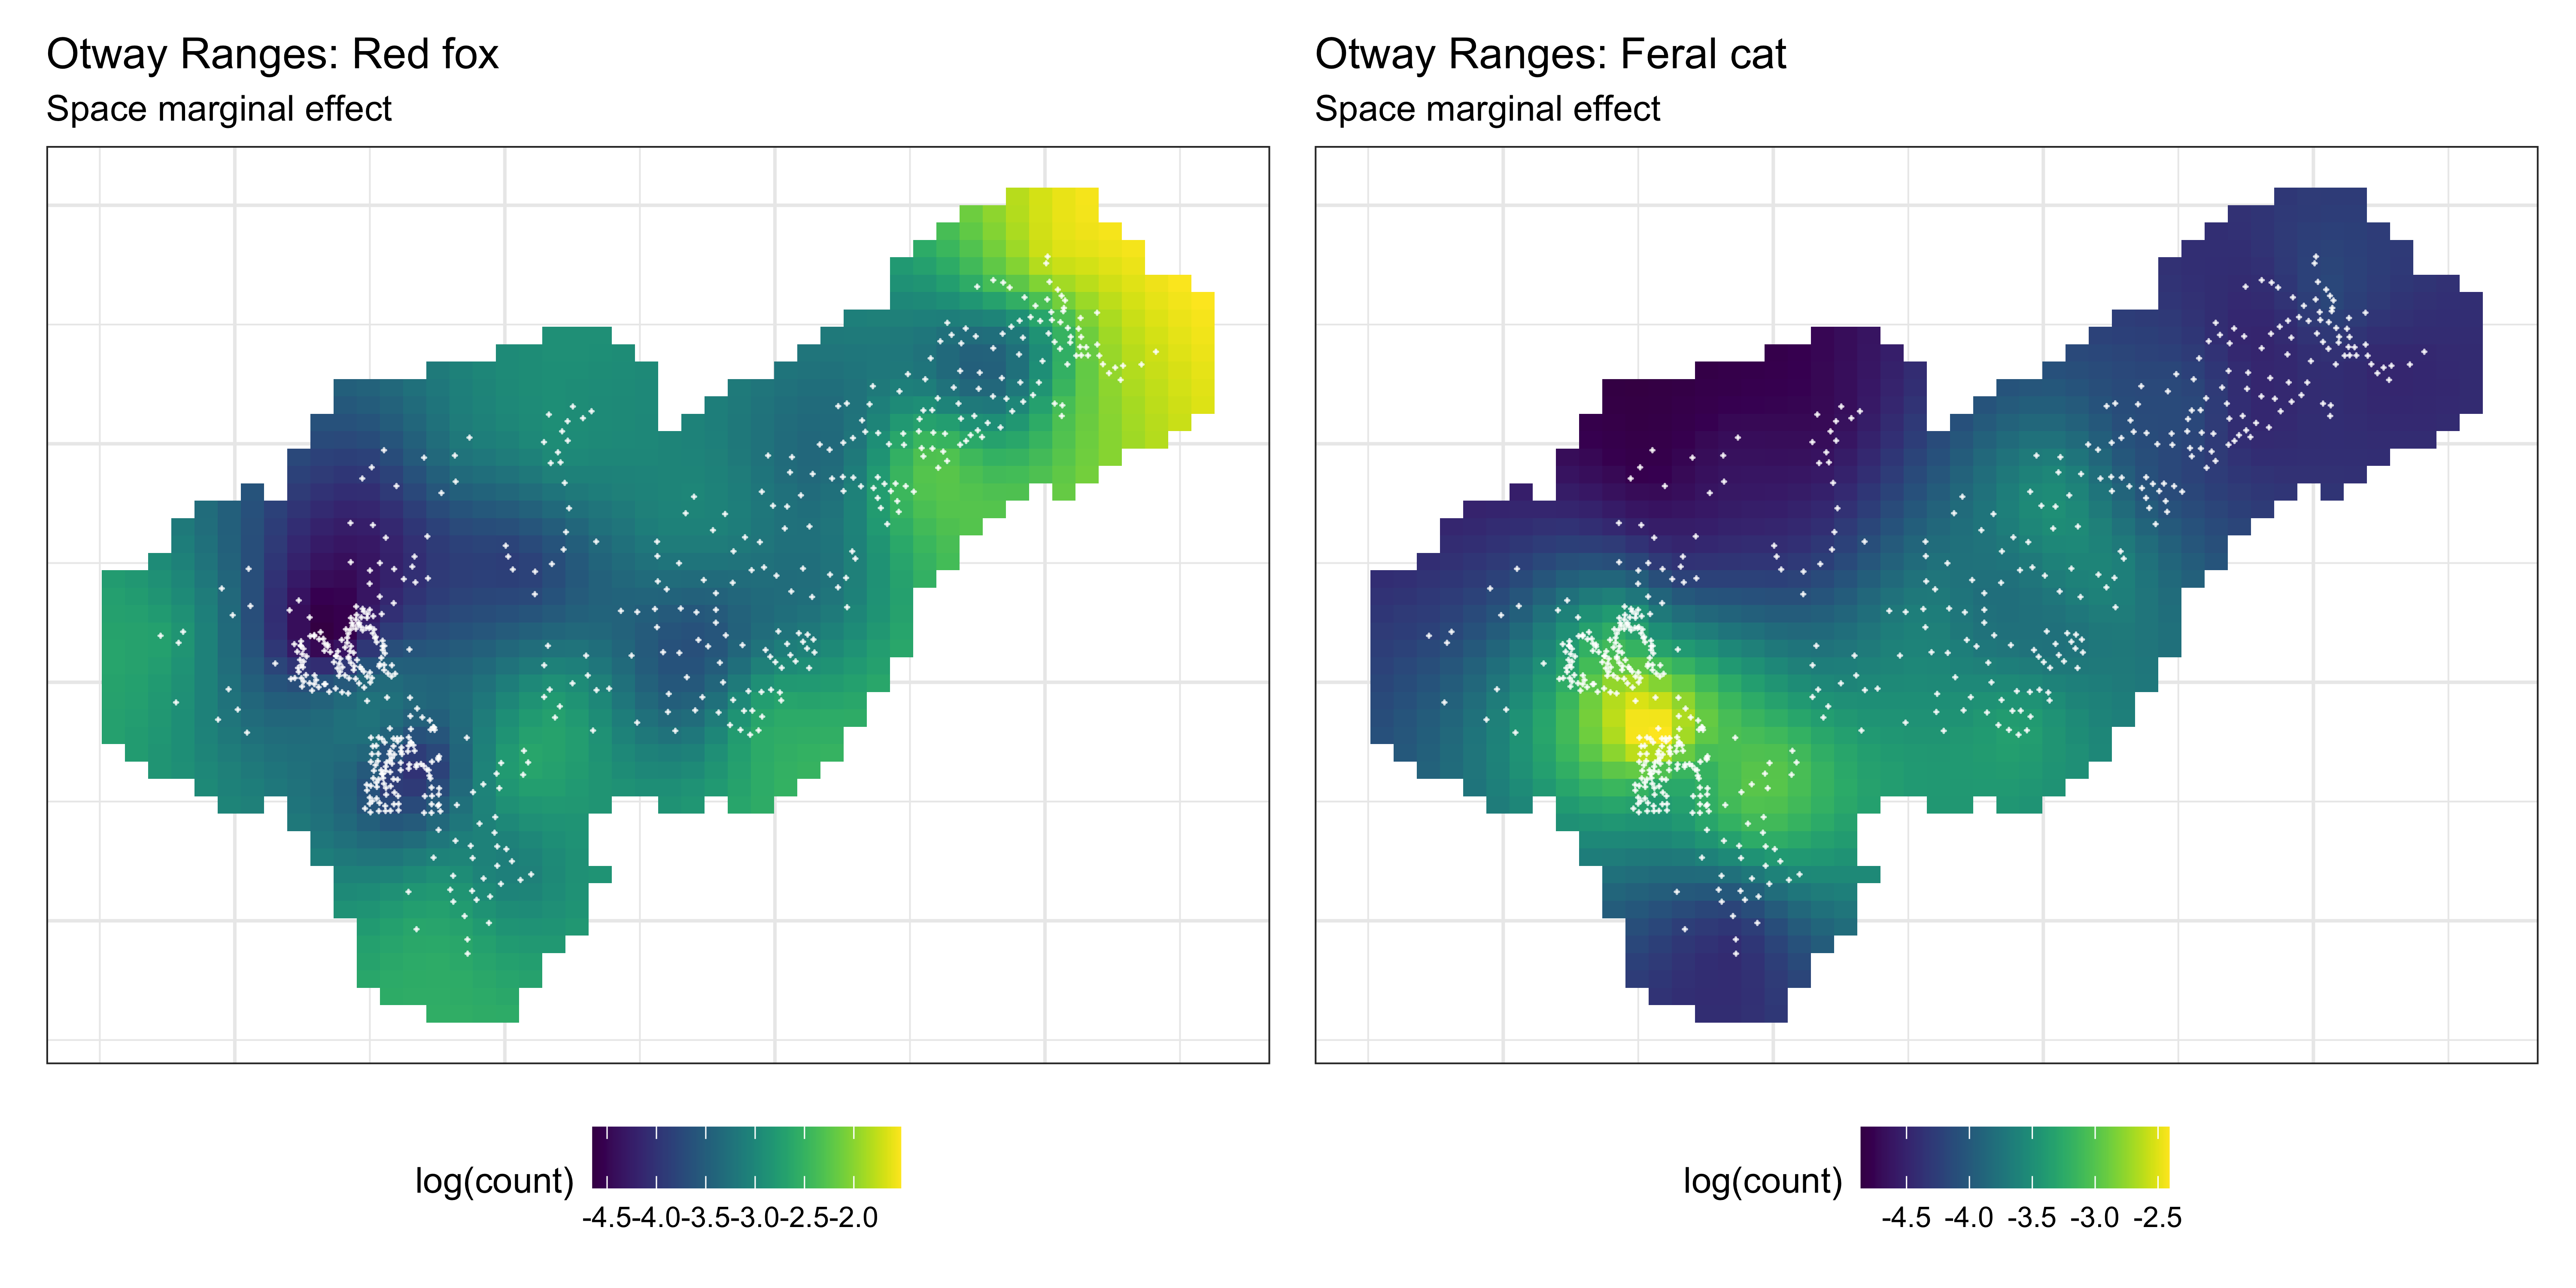
\includegraphics[width=1\linewidth]{figure/sp_marginal_o} 

}

\caption{Marginal effect of space on predators across south-west Victoria, Australia (model 1). White crosses depict unique camera-trap sites}\label{fig:diel-space-time-marginal-o}
\end{figure}
\newpage
\begin{figure}

{\centering 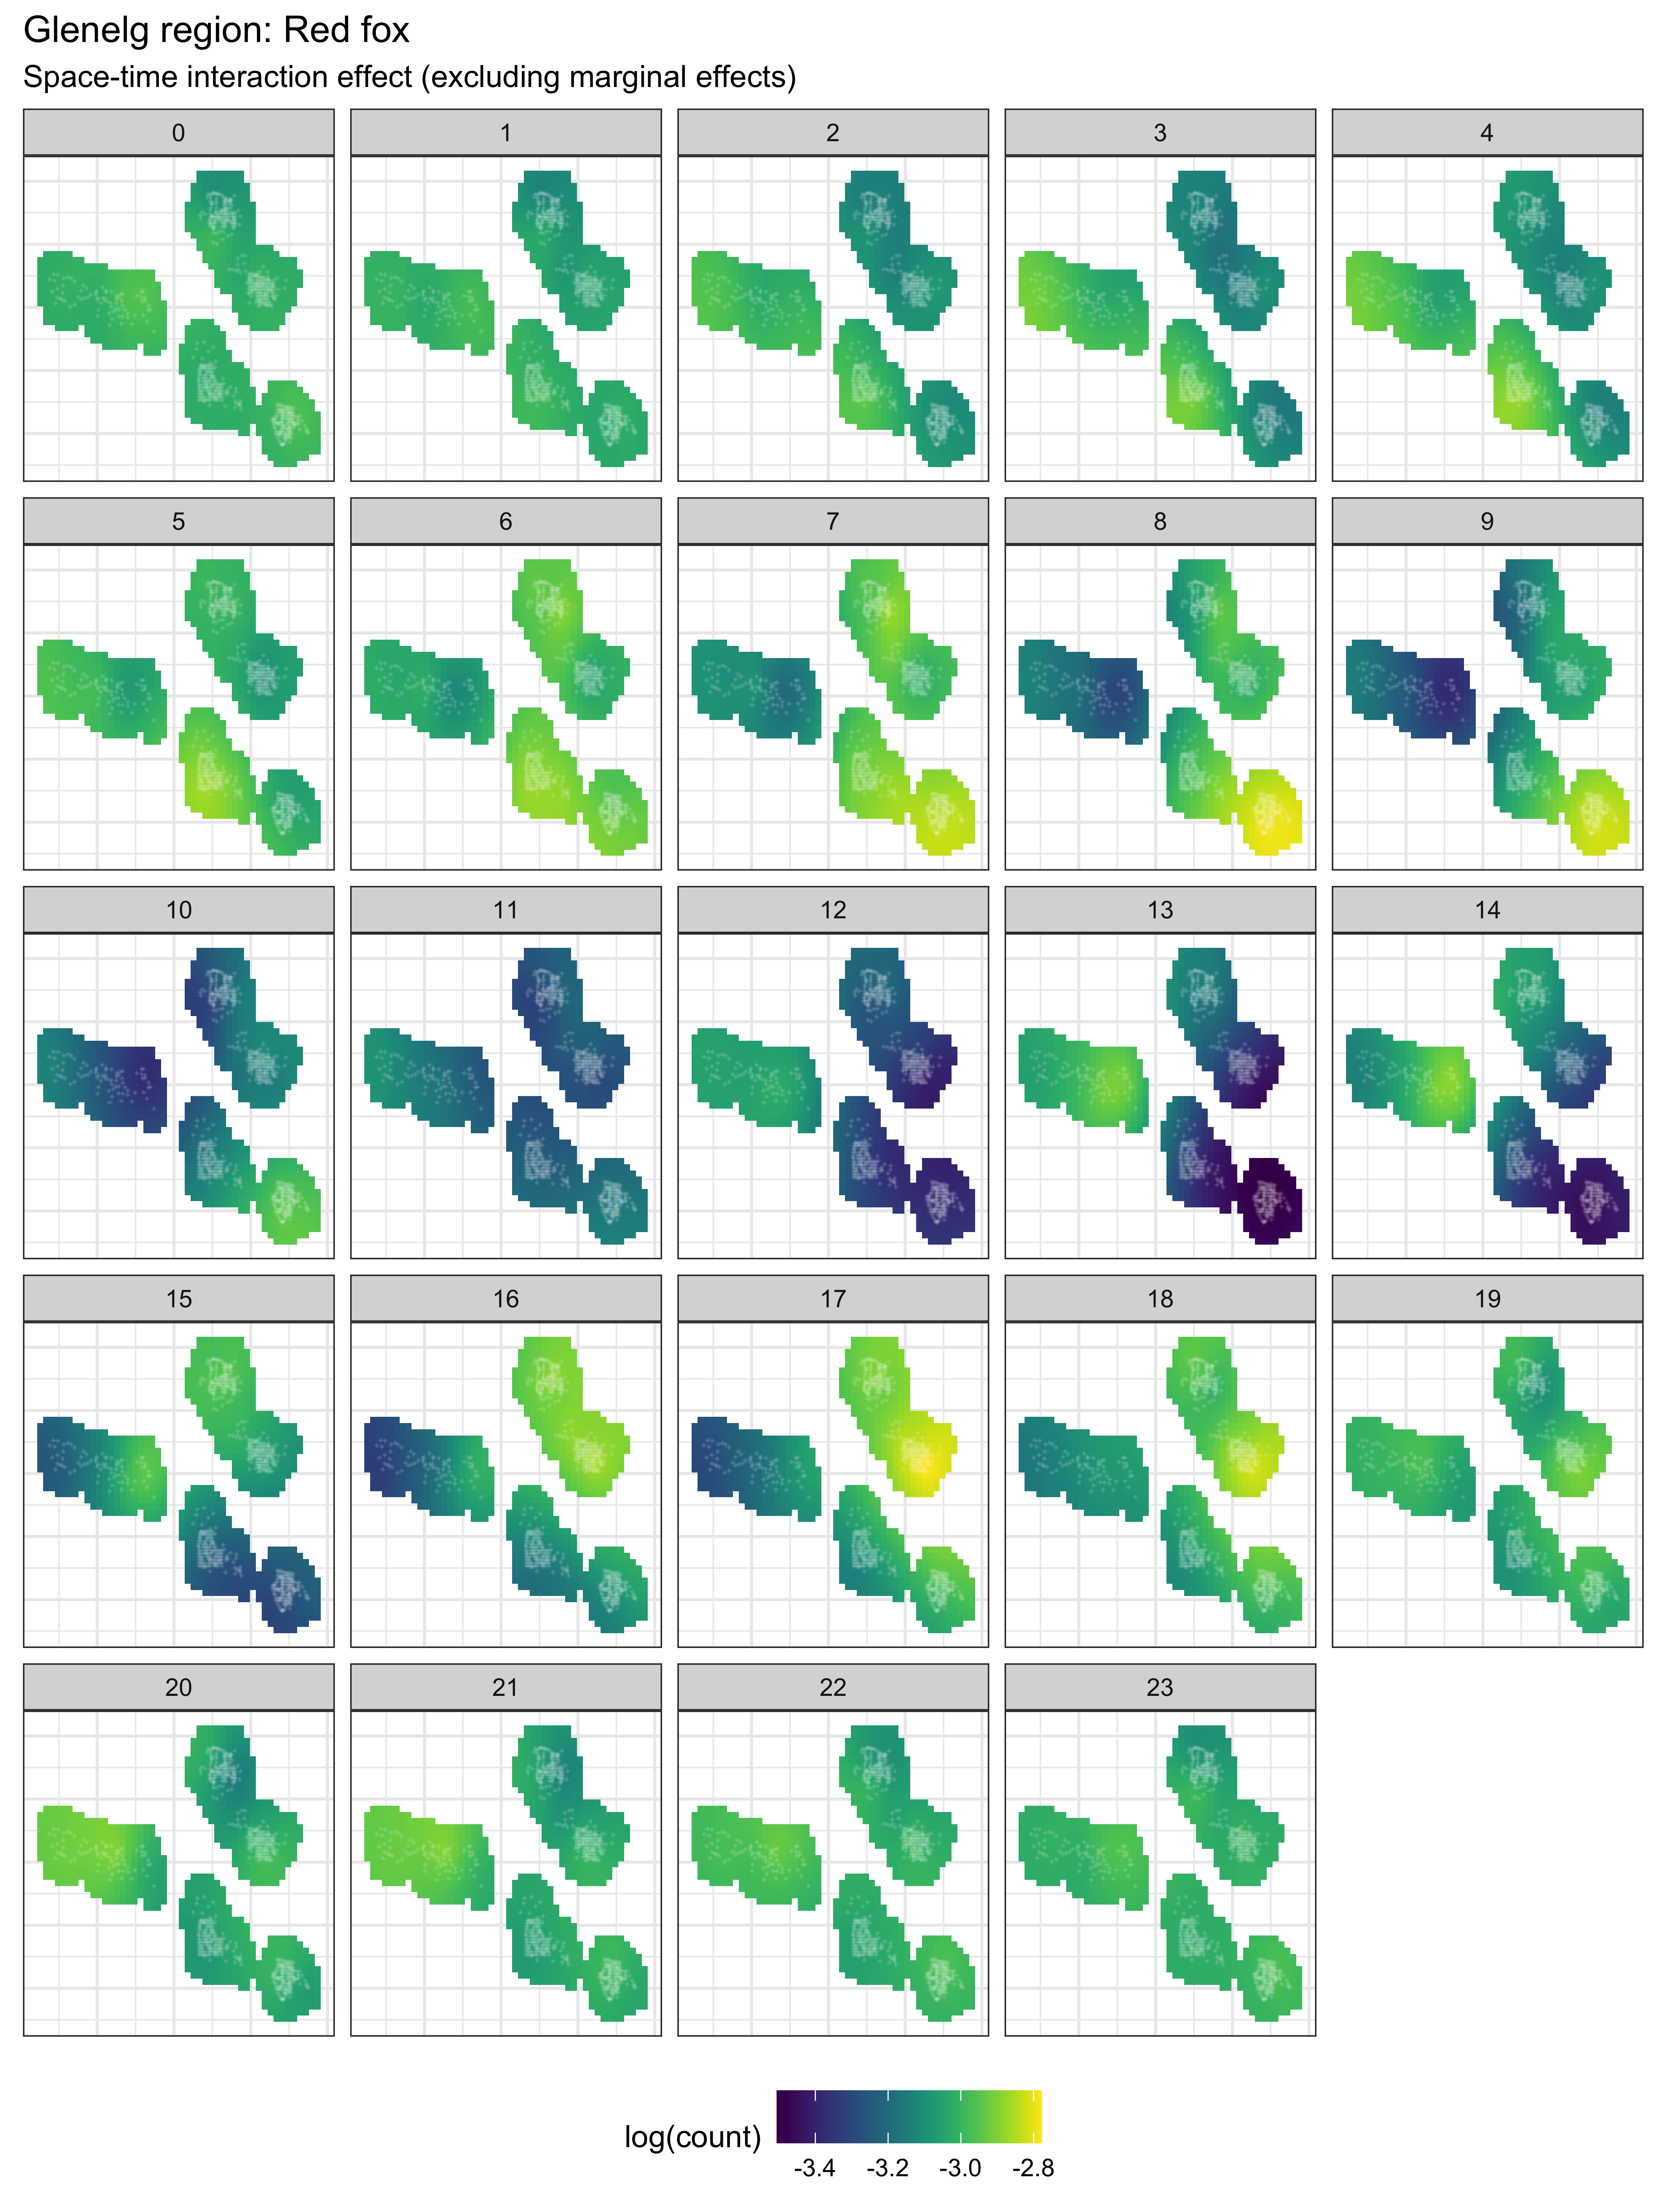
\includegraphics[width=1\linewidth]{figure/spte_diff_avg_g_fox} 

}

\caption{Interaction effect of space-time on feral cat \textit{Felis catus} activity across each hour of the day (0 - 23) in the Glenelg region, Australia (model 1). White crosses depict unique camera-trap sites. }\label{fig:diel-st-int-g-fox}
\end{figure}
\newpage
\begin{figure}

{\centering 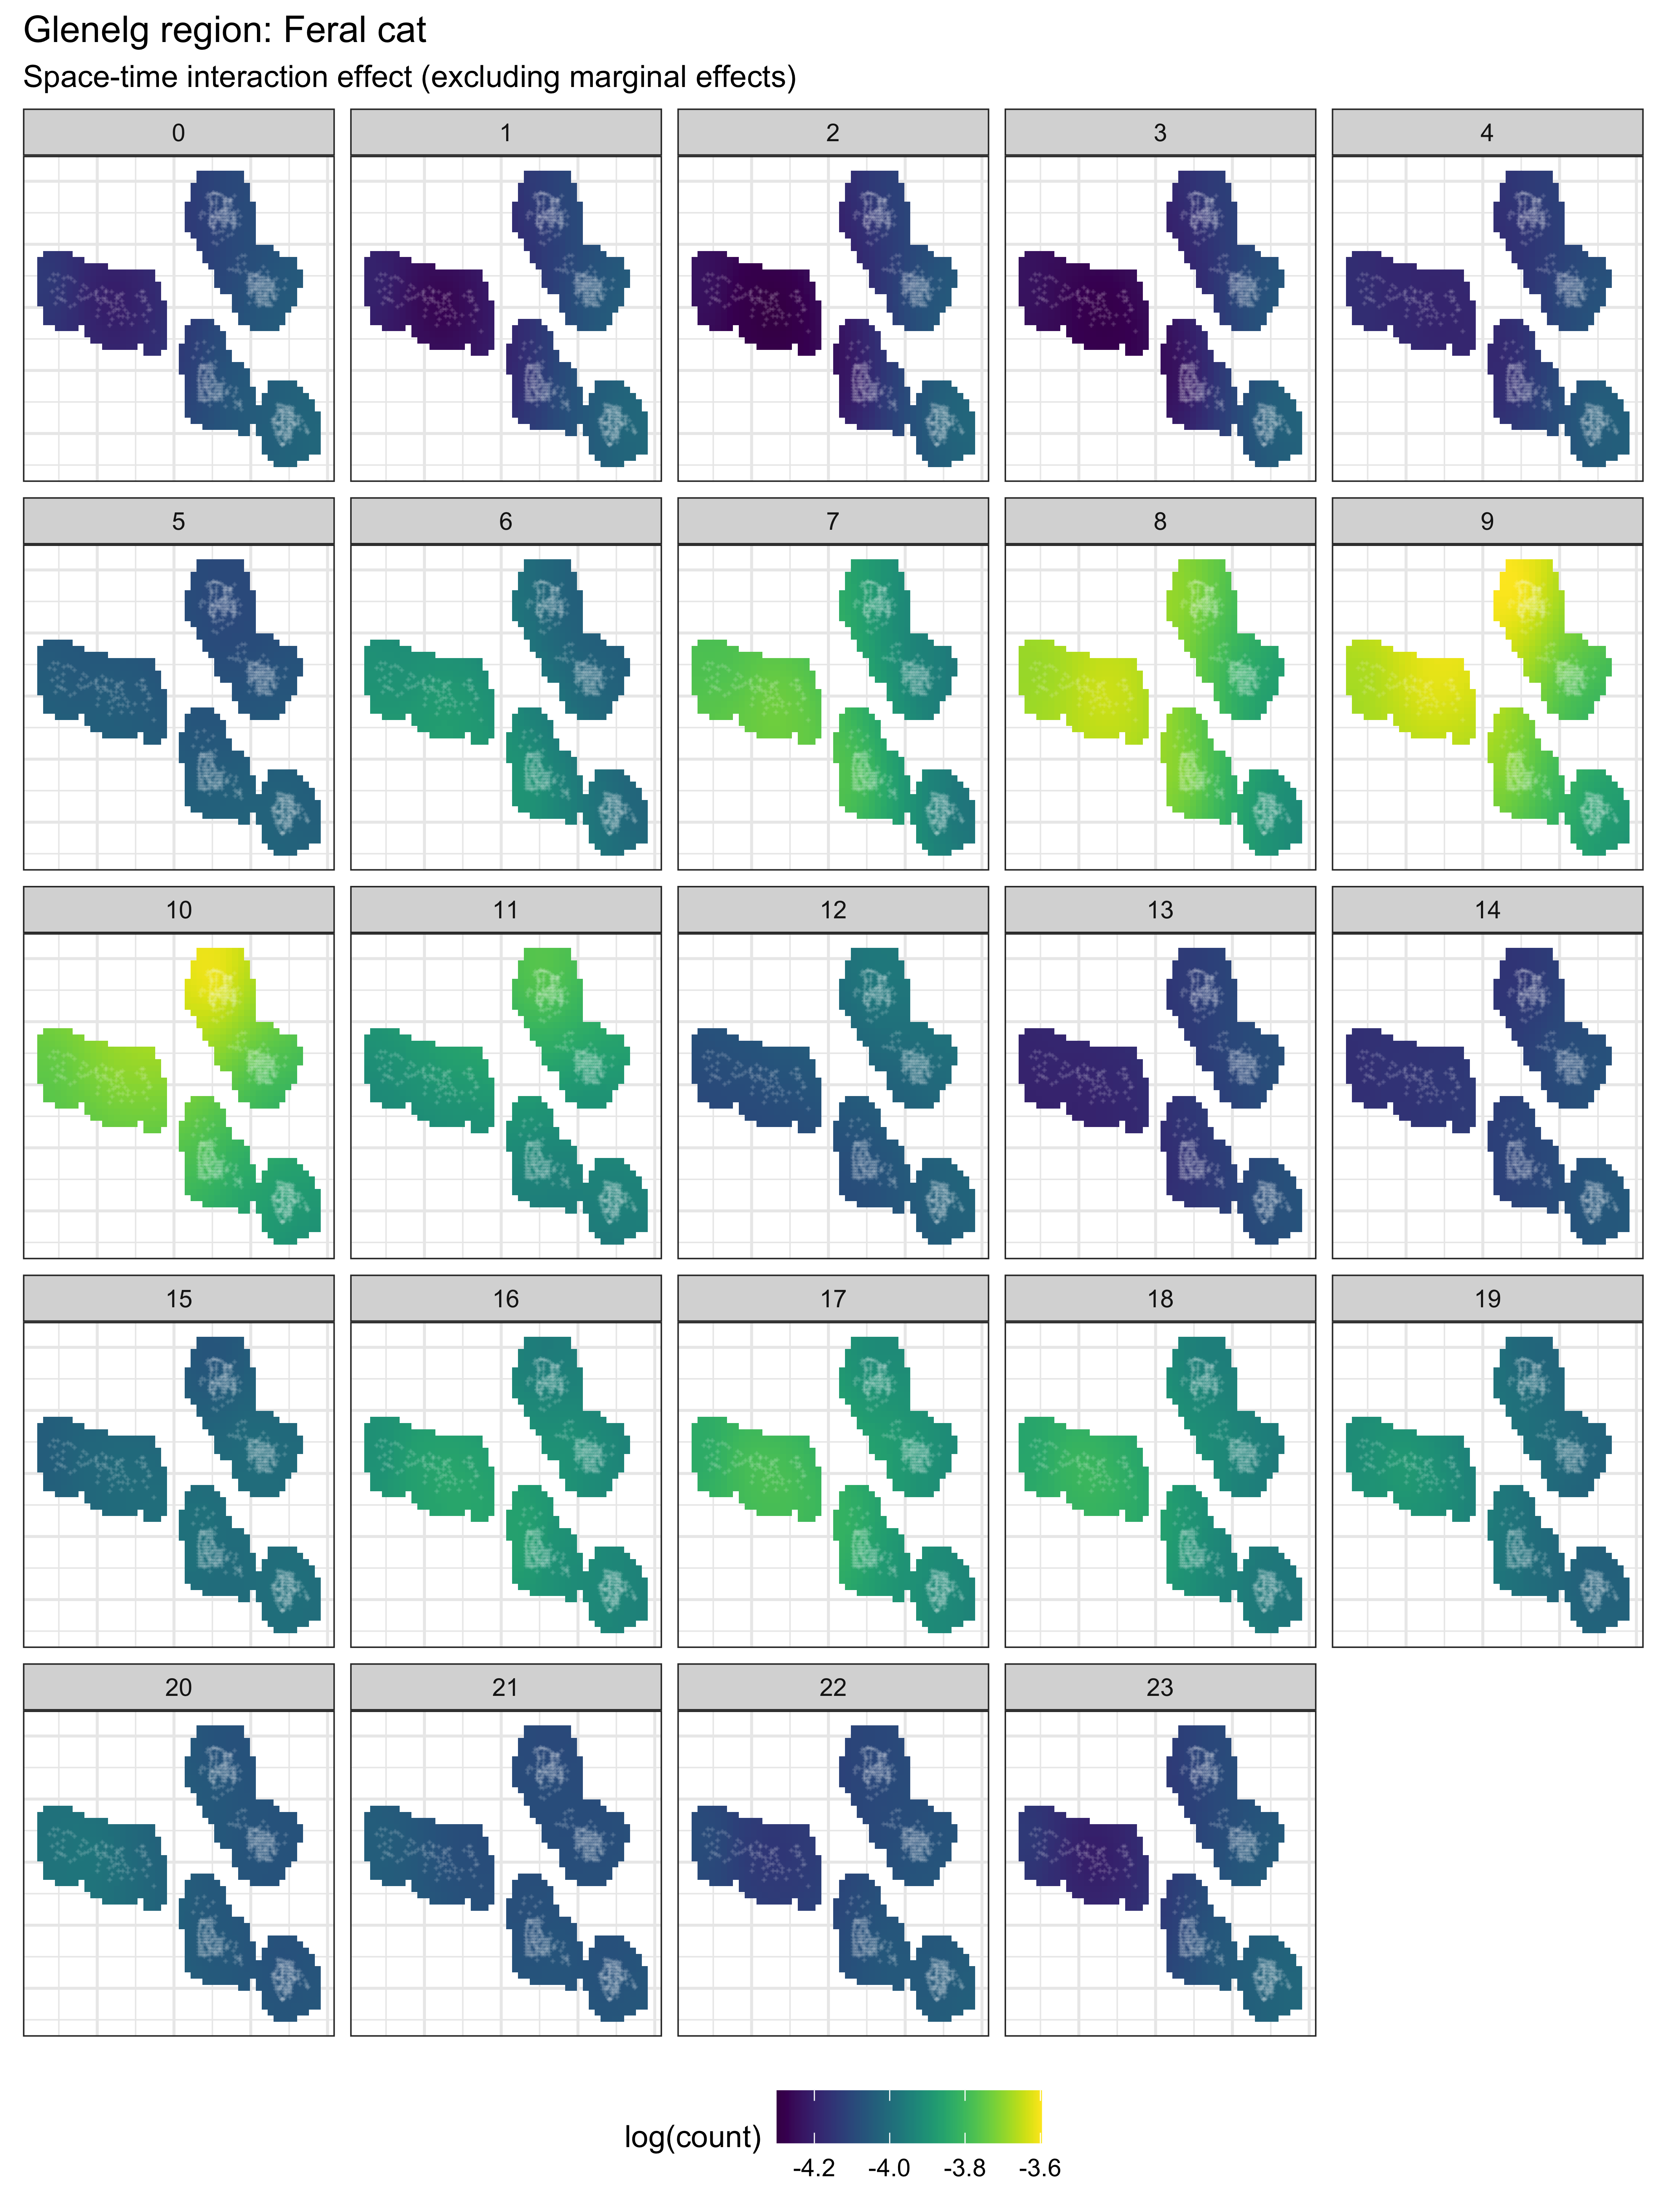
\includegraphics[width=1\linewidth]{figure/spte_diff_avg_g_cat} 

}

\caption{Interaction effect of space-time on feral cat \textit{Felis catus} activity across each hour of the day (0 - 23) in the Glenelg region, Australia (model 1). White crosses depict unique camera-trap sites. }\label{fig:diel-st-int-g-cat}
\end{figure}
\newpage
\begin{figure}

{\centering 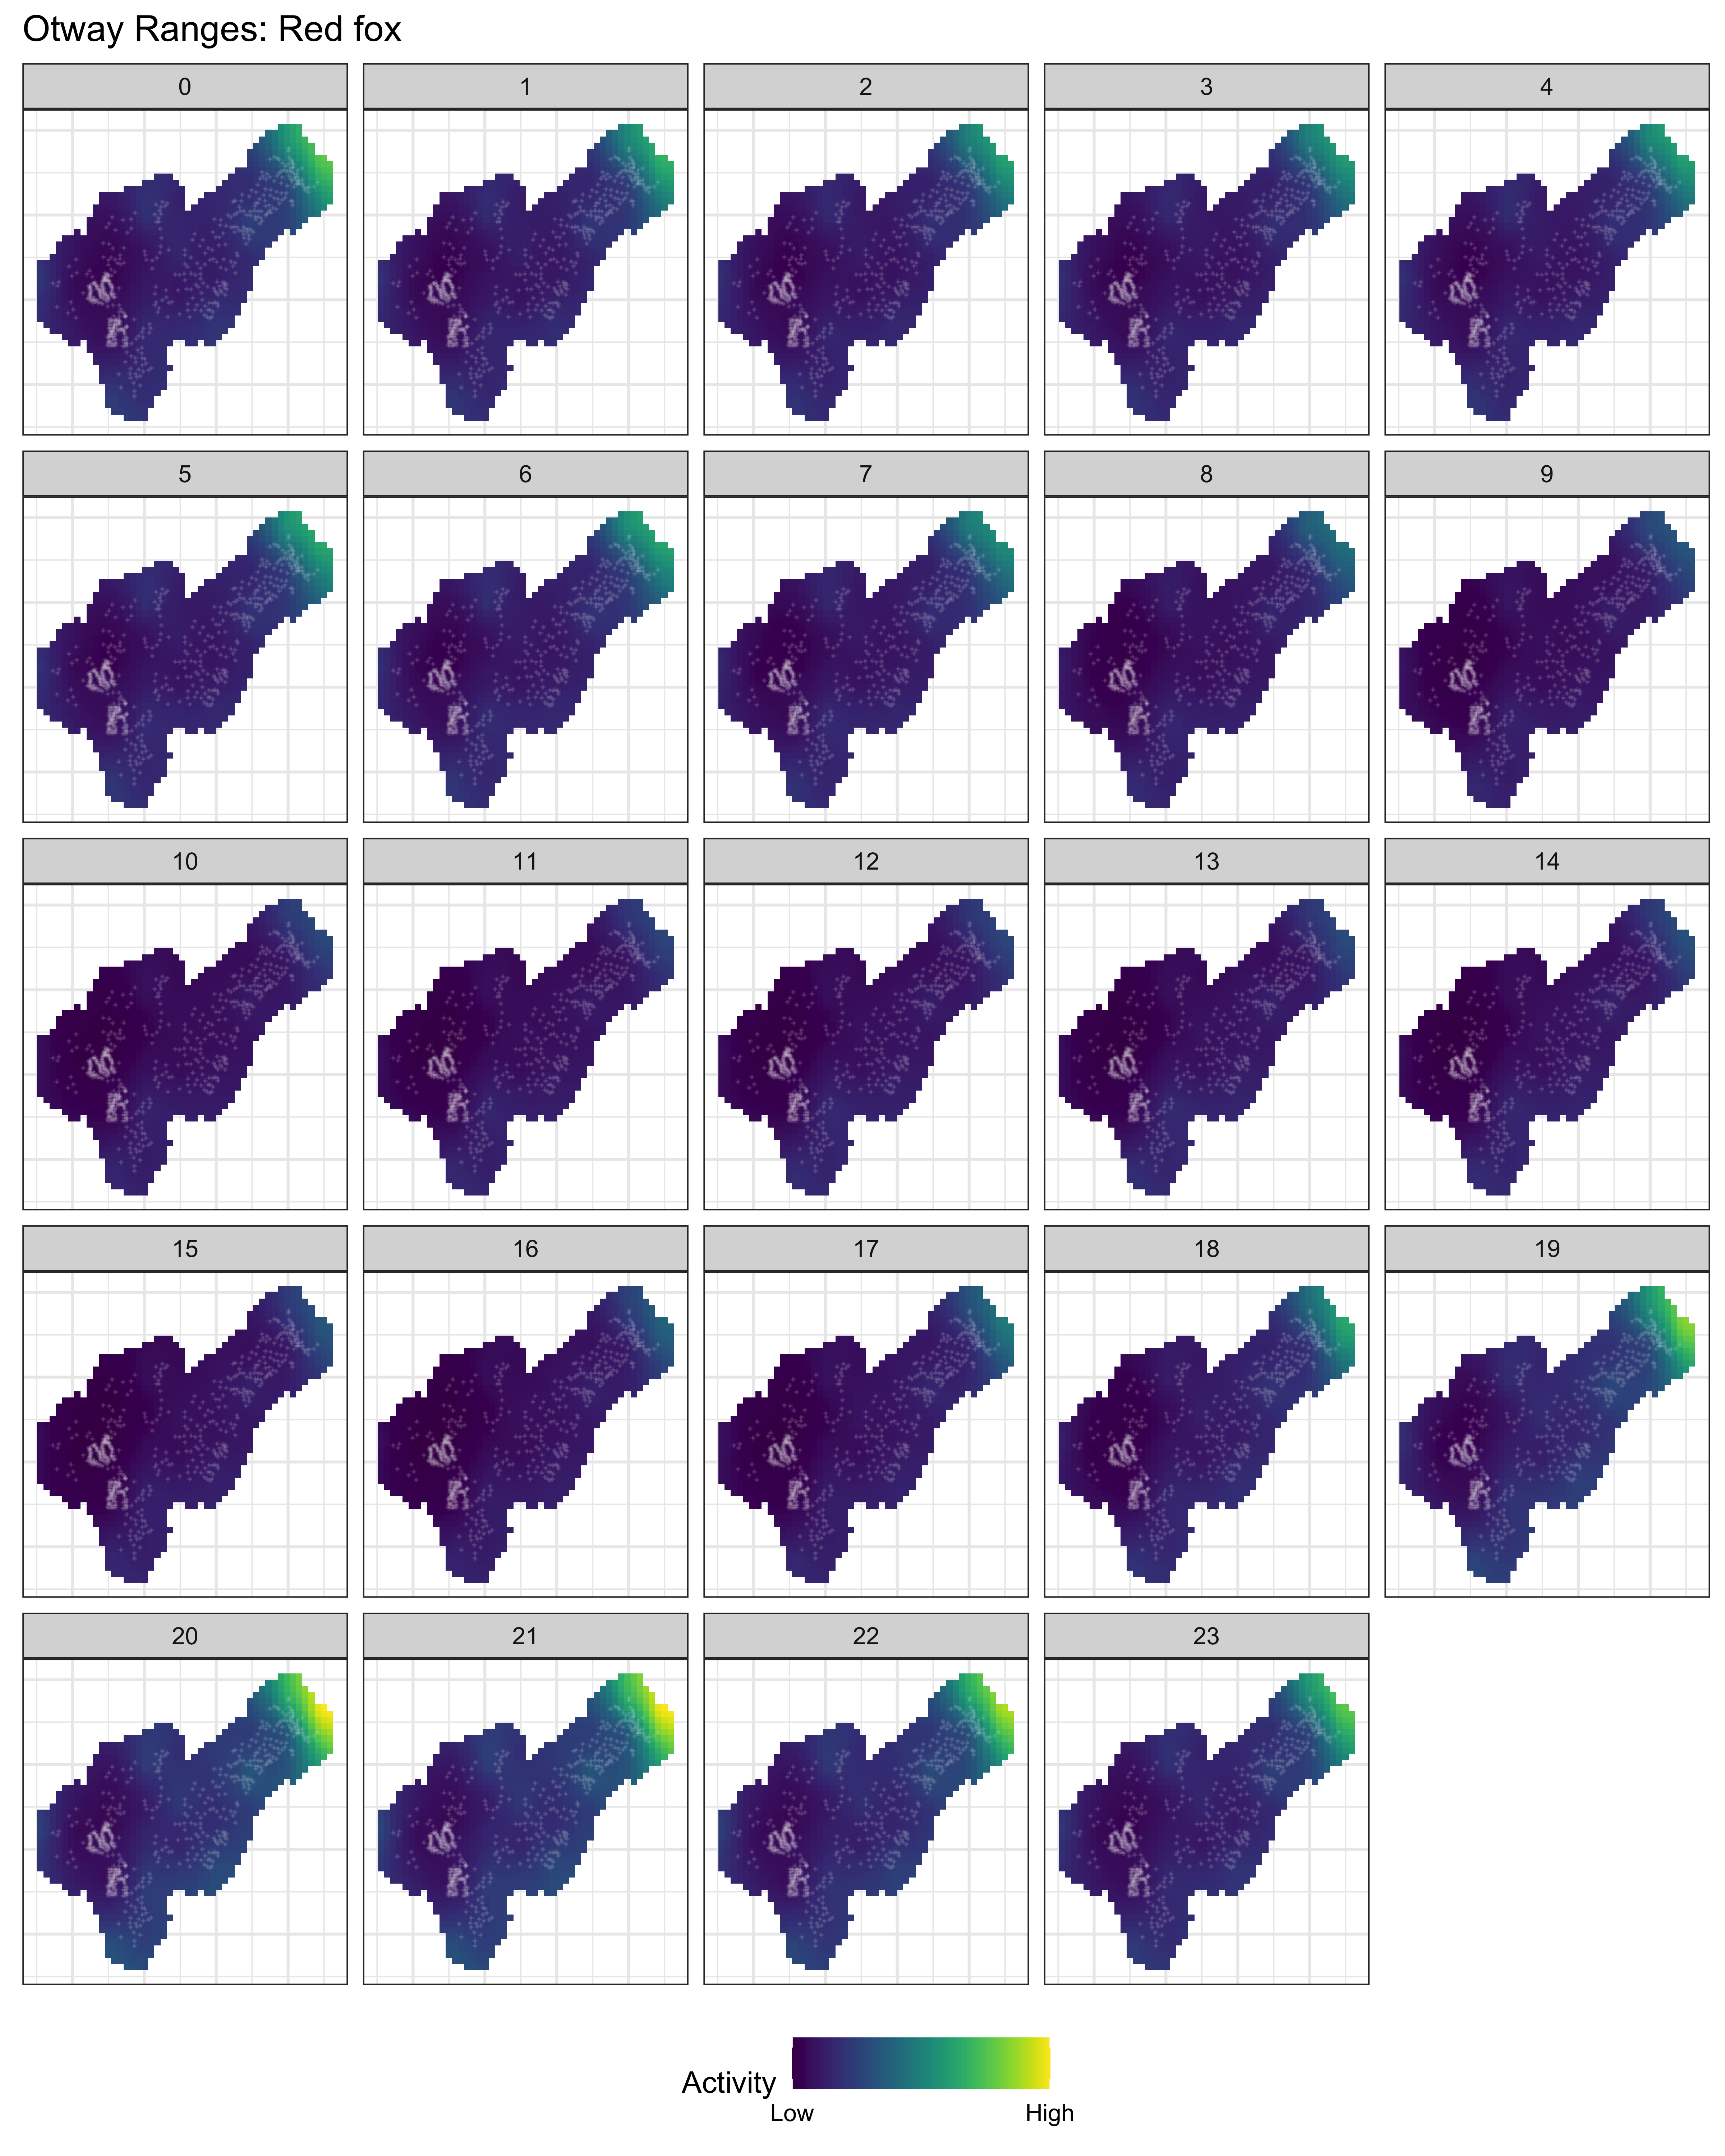
\includegraphics[width=1\linewidth]{figure/spte_facet_o_fox} 

}

\caption{Overall spatial activity of red foxes \textit{Vulpes vulpes} for each hour of the day (0 - 23) in the Glenelg region, Australia (model 1). White crosses depict unique camera-trap sites}\label{fig:diel-space-g-fox}
\end{figure}
\newpage
\begin{figure}

{\centering 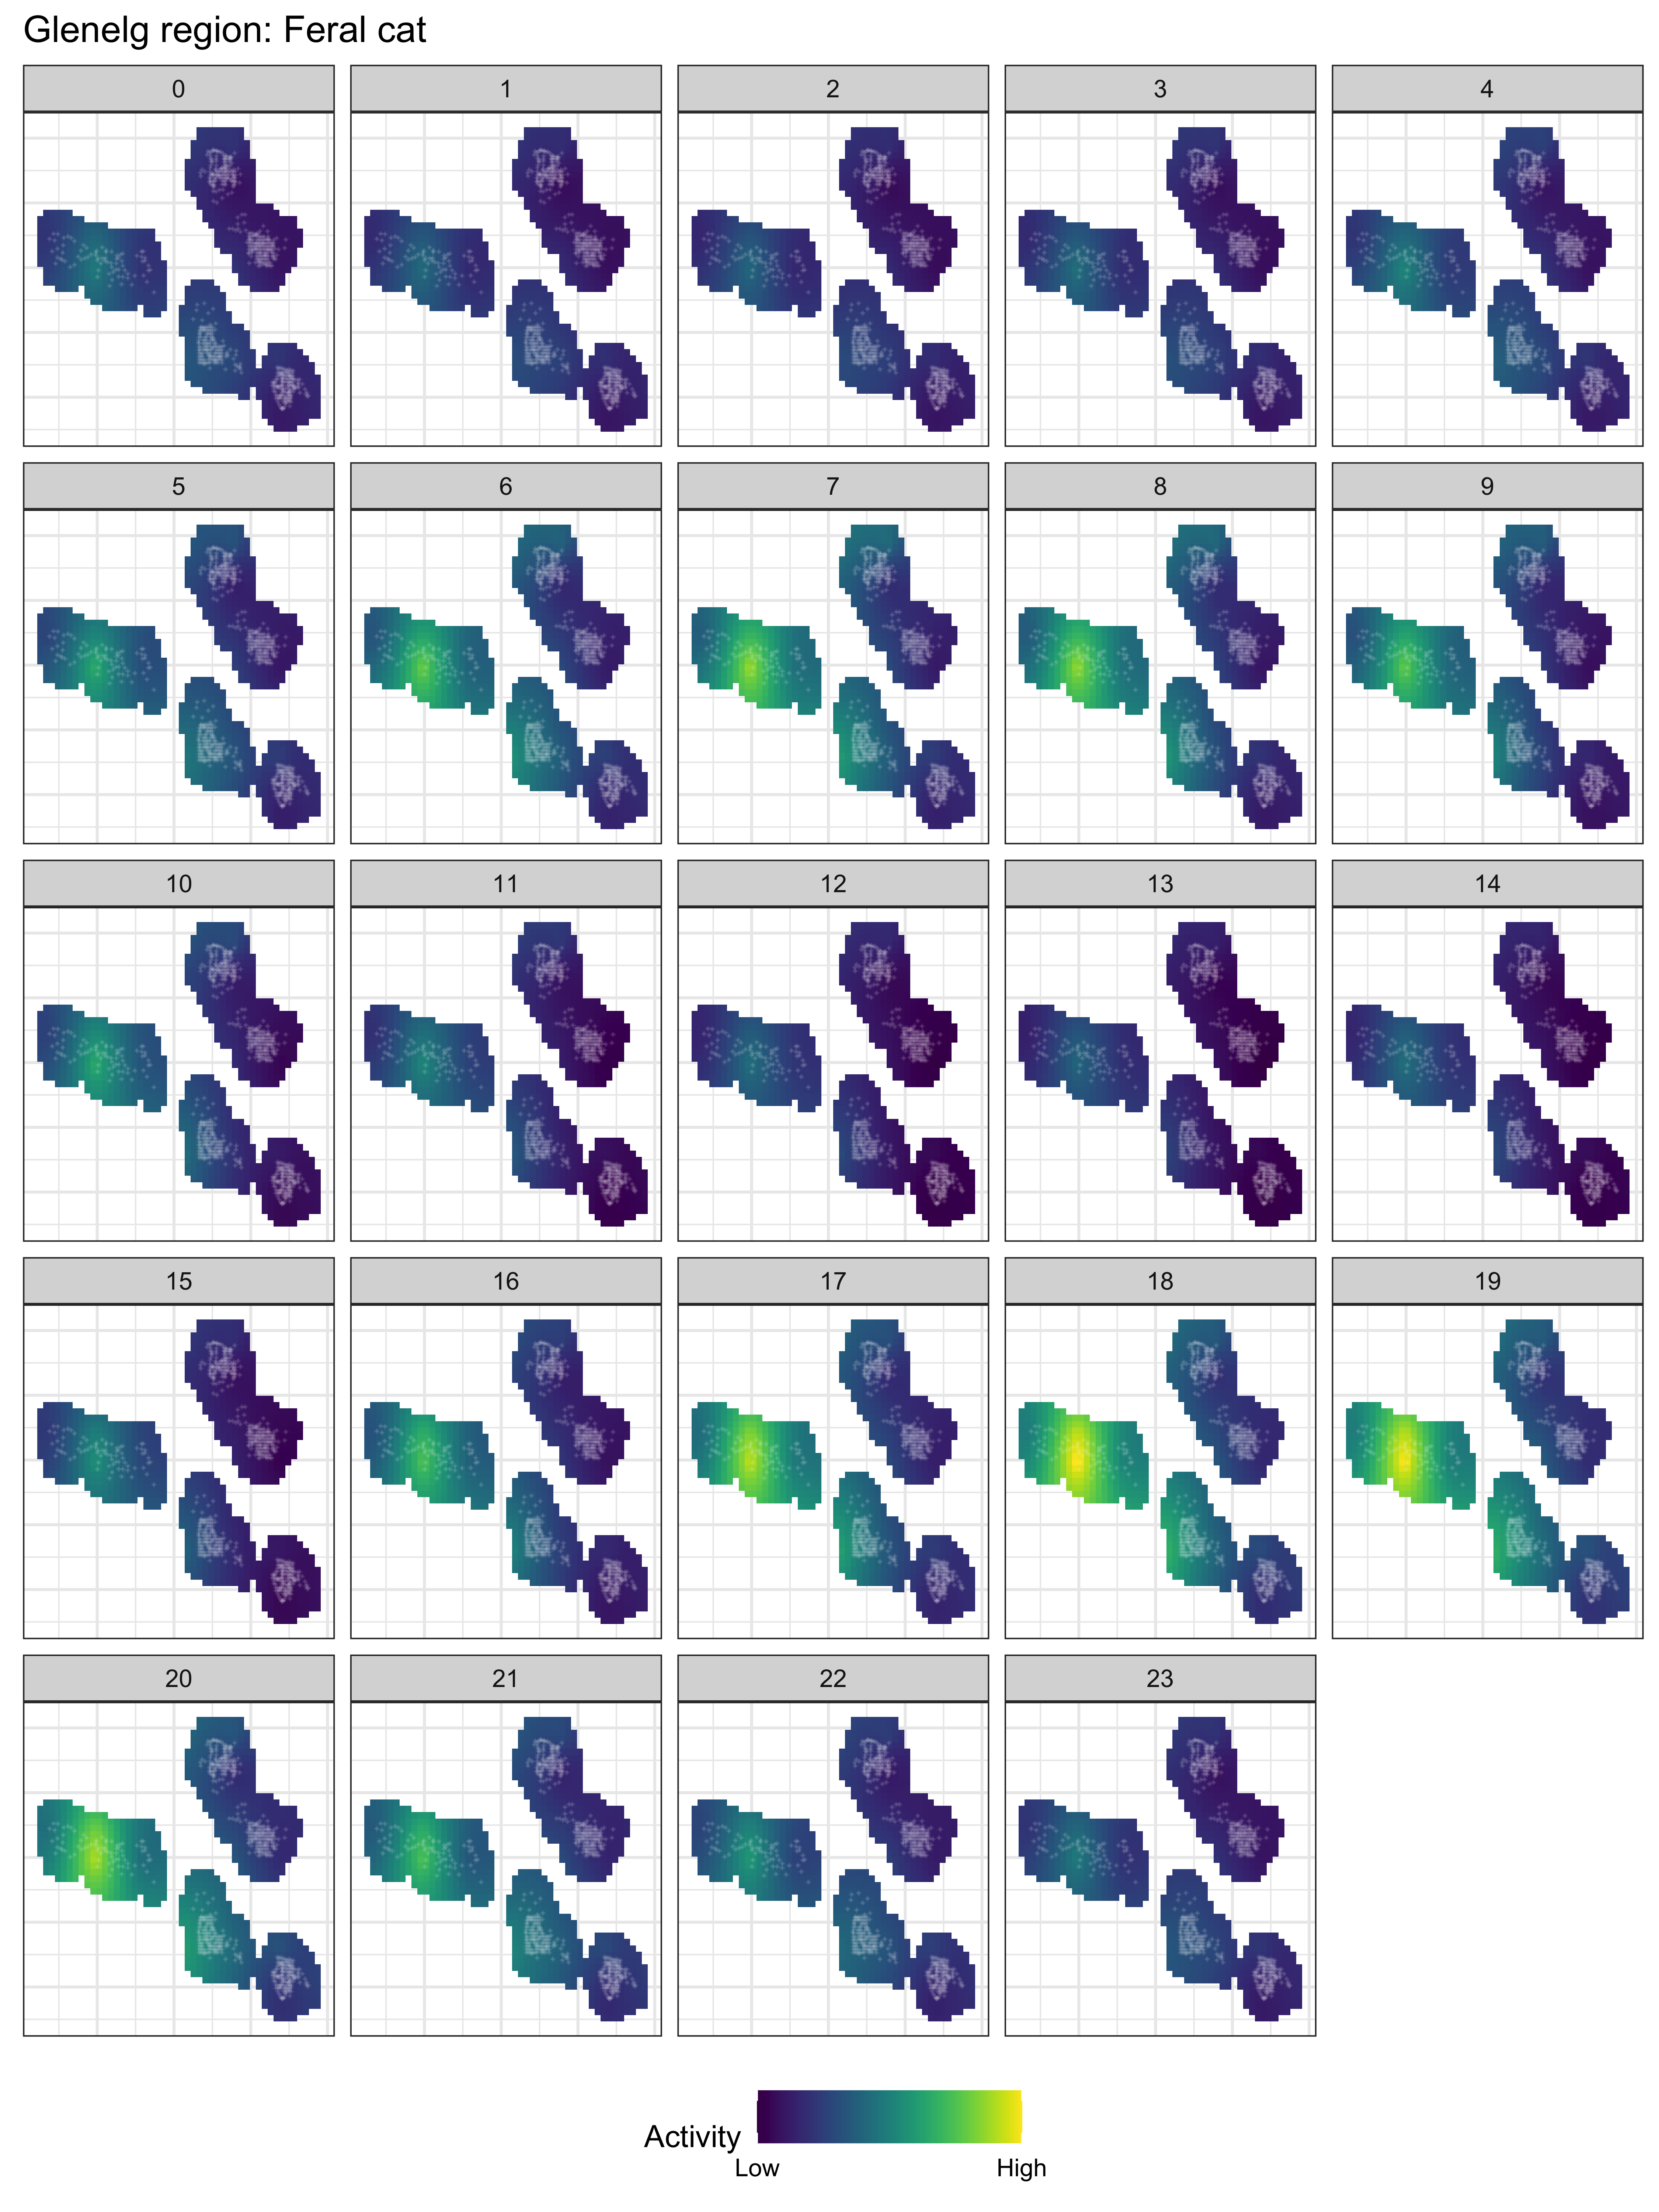
\includegraphics[width=1\linewidth]{figure/spte_facet_g_cat} 

}

\caption{Overall spatial activity of feral cats \textit{Felis catus} for each hour of the day (0 - 23) in the Glenelg region, Australia (model 1). White crosses depict unique camera-trap sites}\label{fig:diel-space-g-cat}
\end{figure}
\newpage
\begin{figure}

{\centering 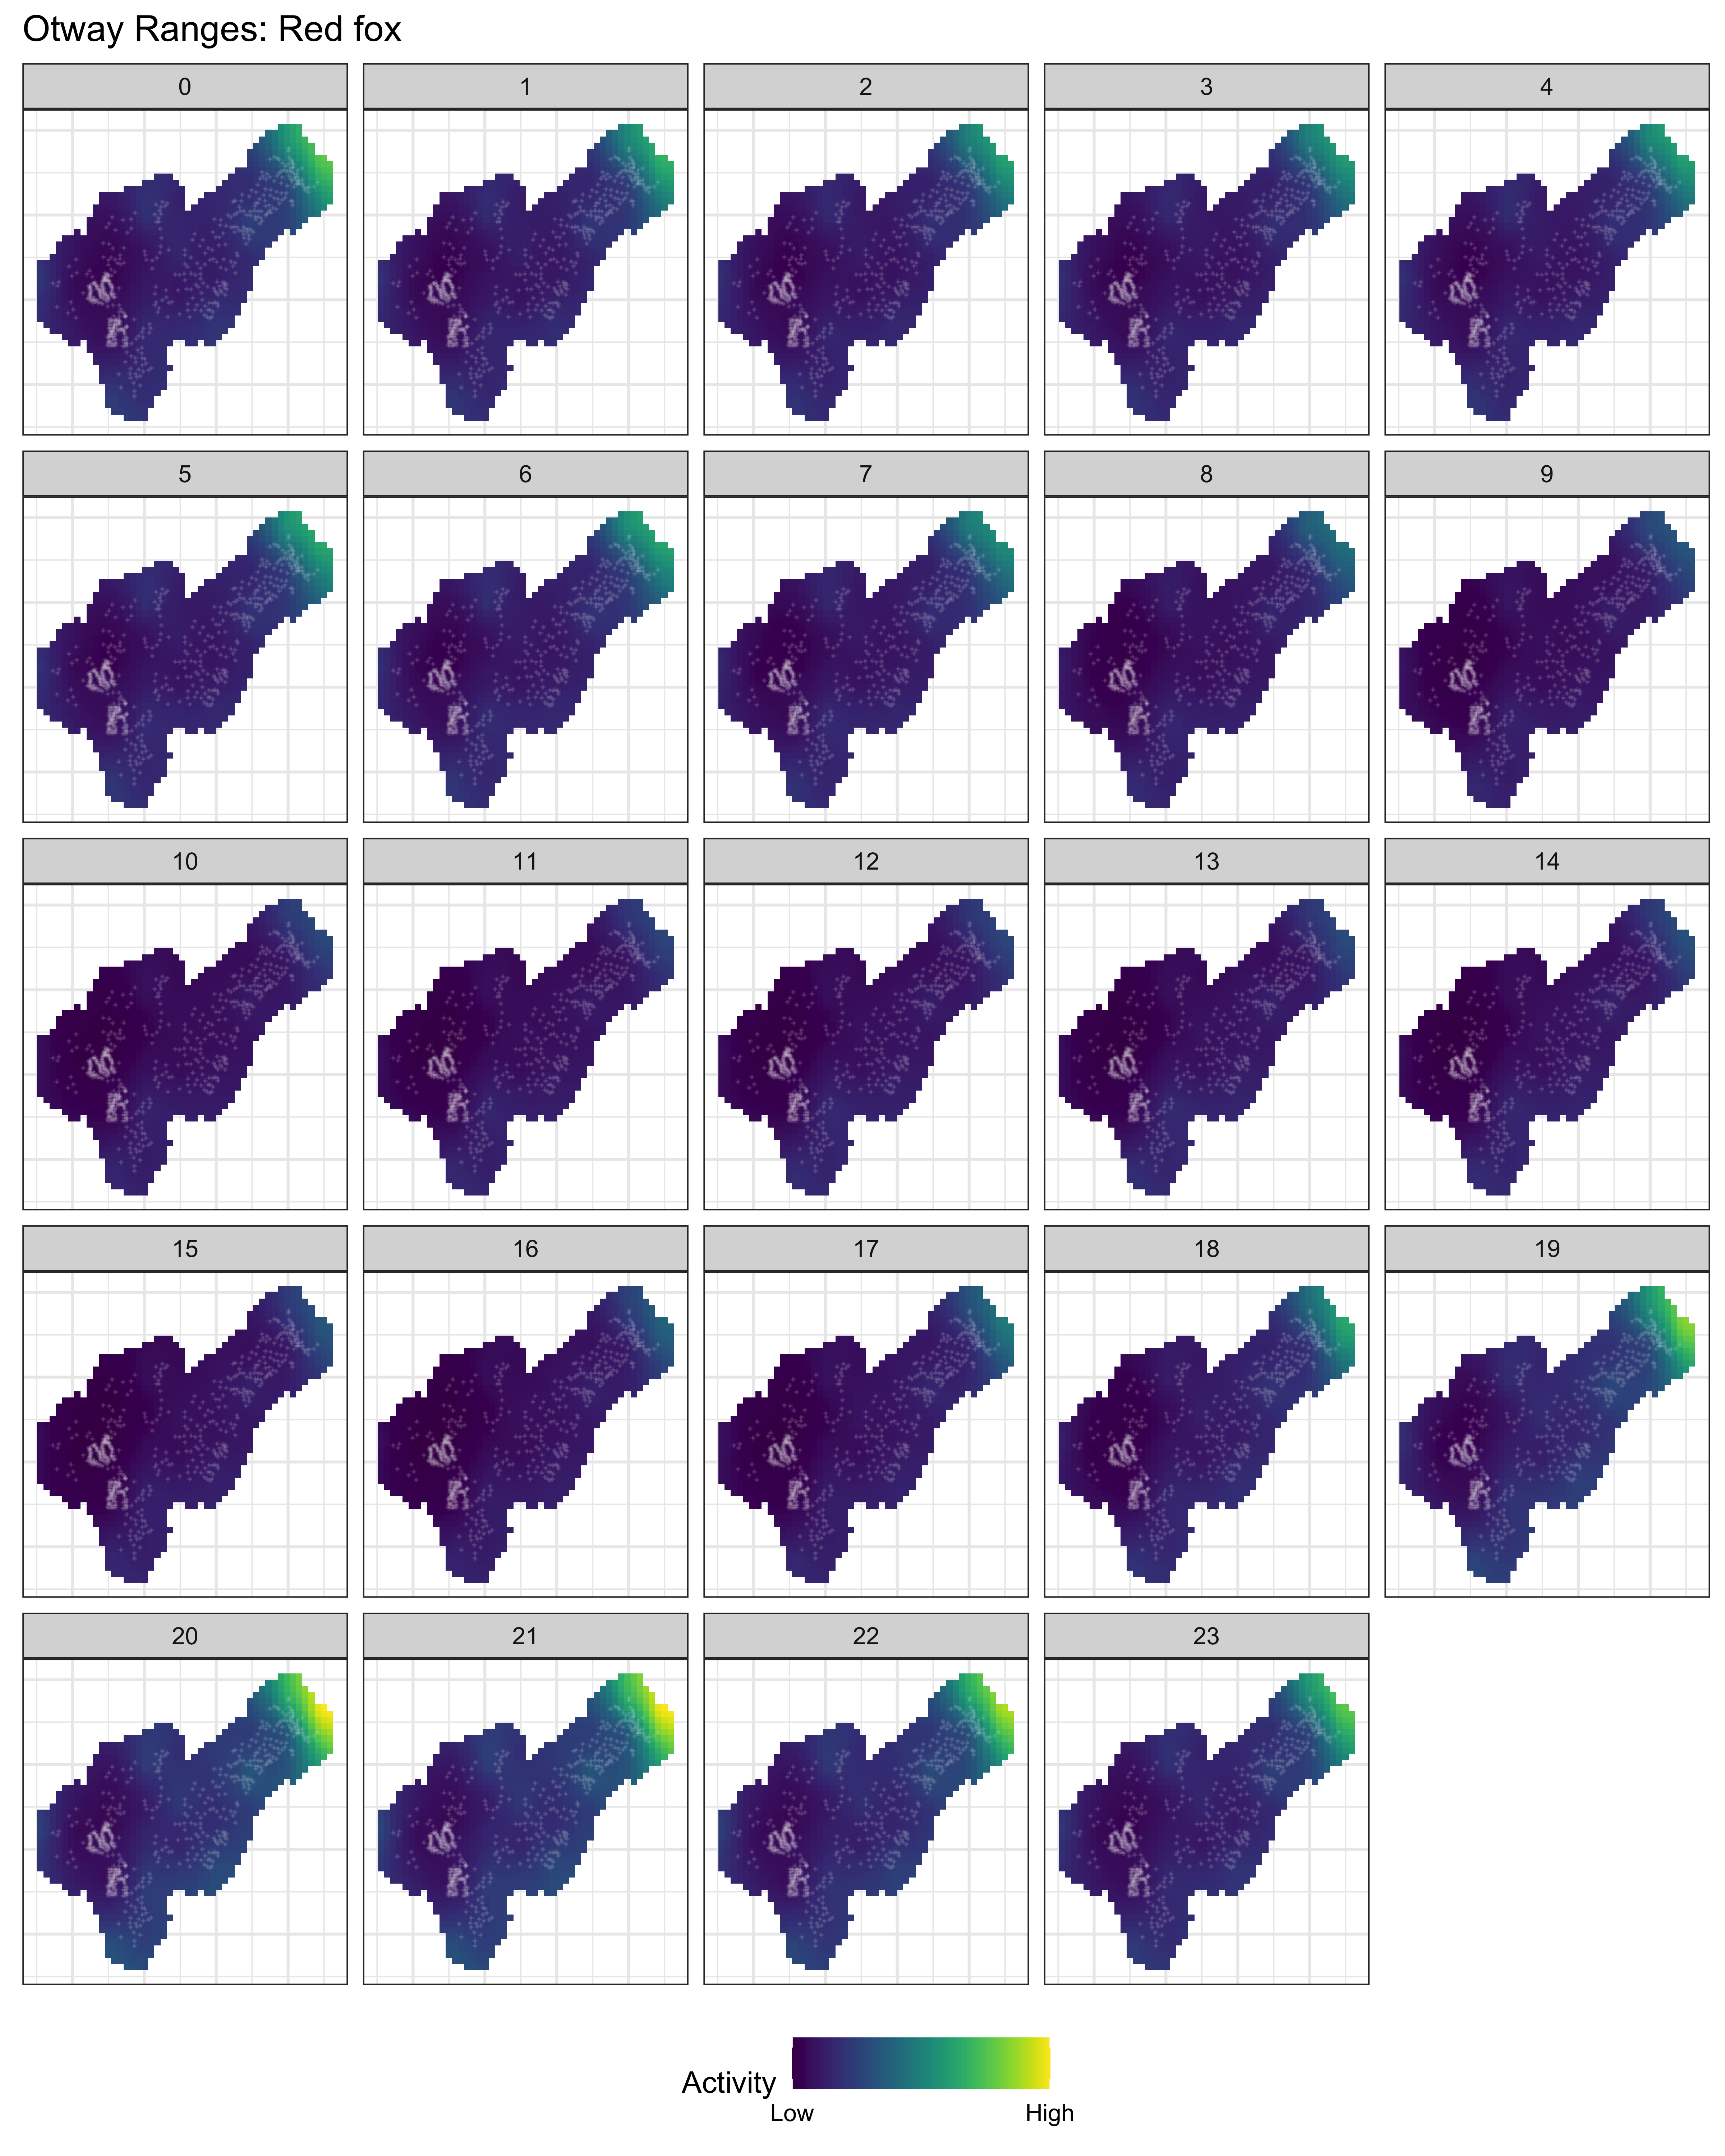
\includegraphics[width=1\linewidth]{figure/spte_facet_o_fox} 

}

\caption{Overall spatial activity of red foxes \textit{Vulpes vulpes} for each hour of the day (0 - 23) in the Otway Ranges, Australia (model 1). White crosses depict unique camera-trap sites}\label{fig:diel-space-o-fox}
\end{figure}
\newpage
\begin{figure}

{\centering 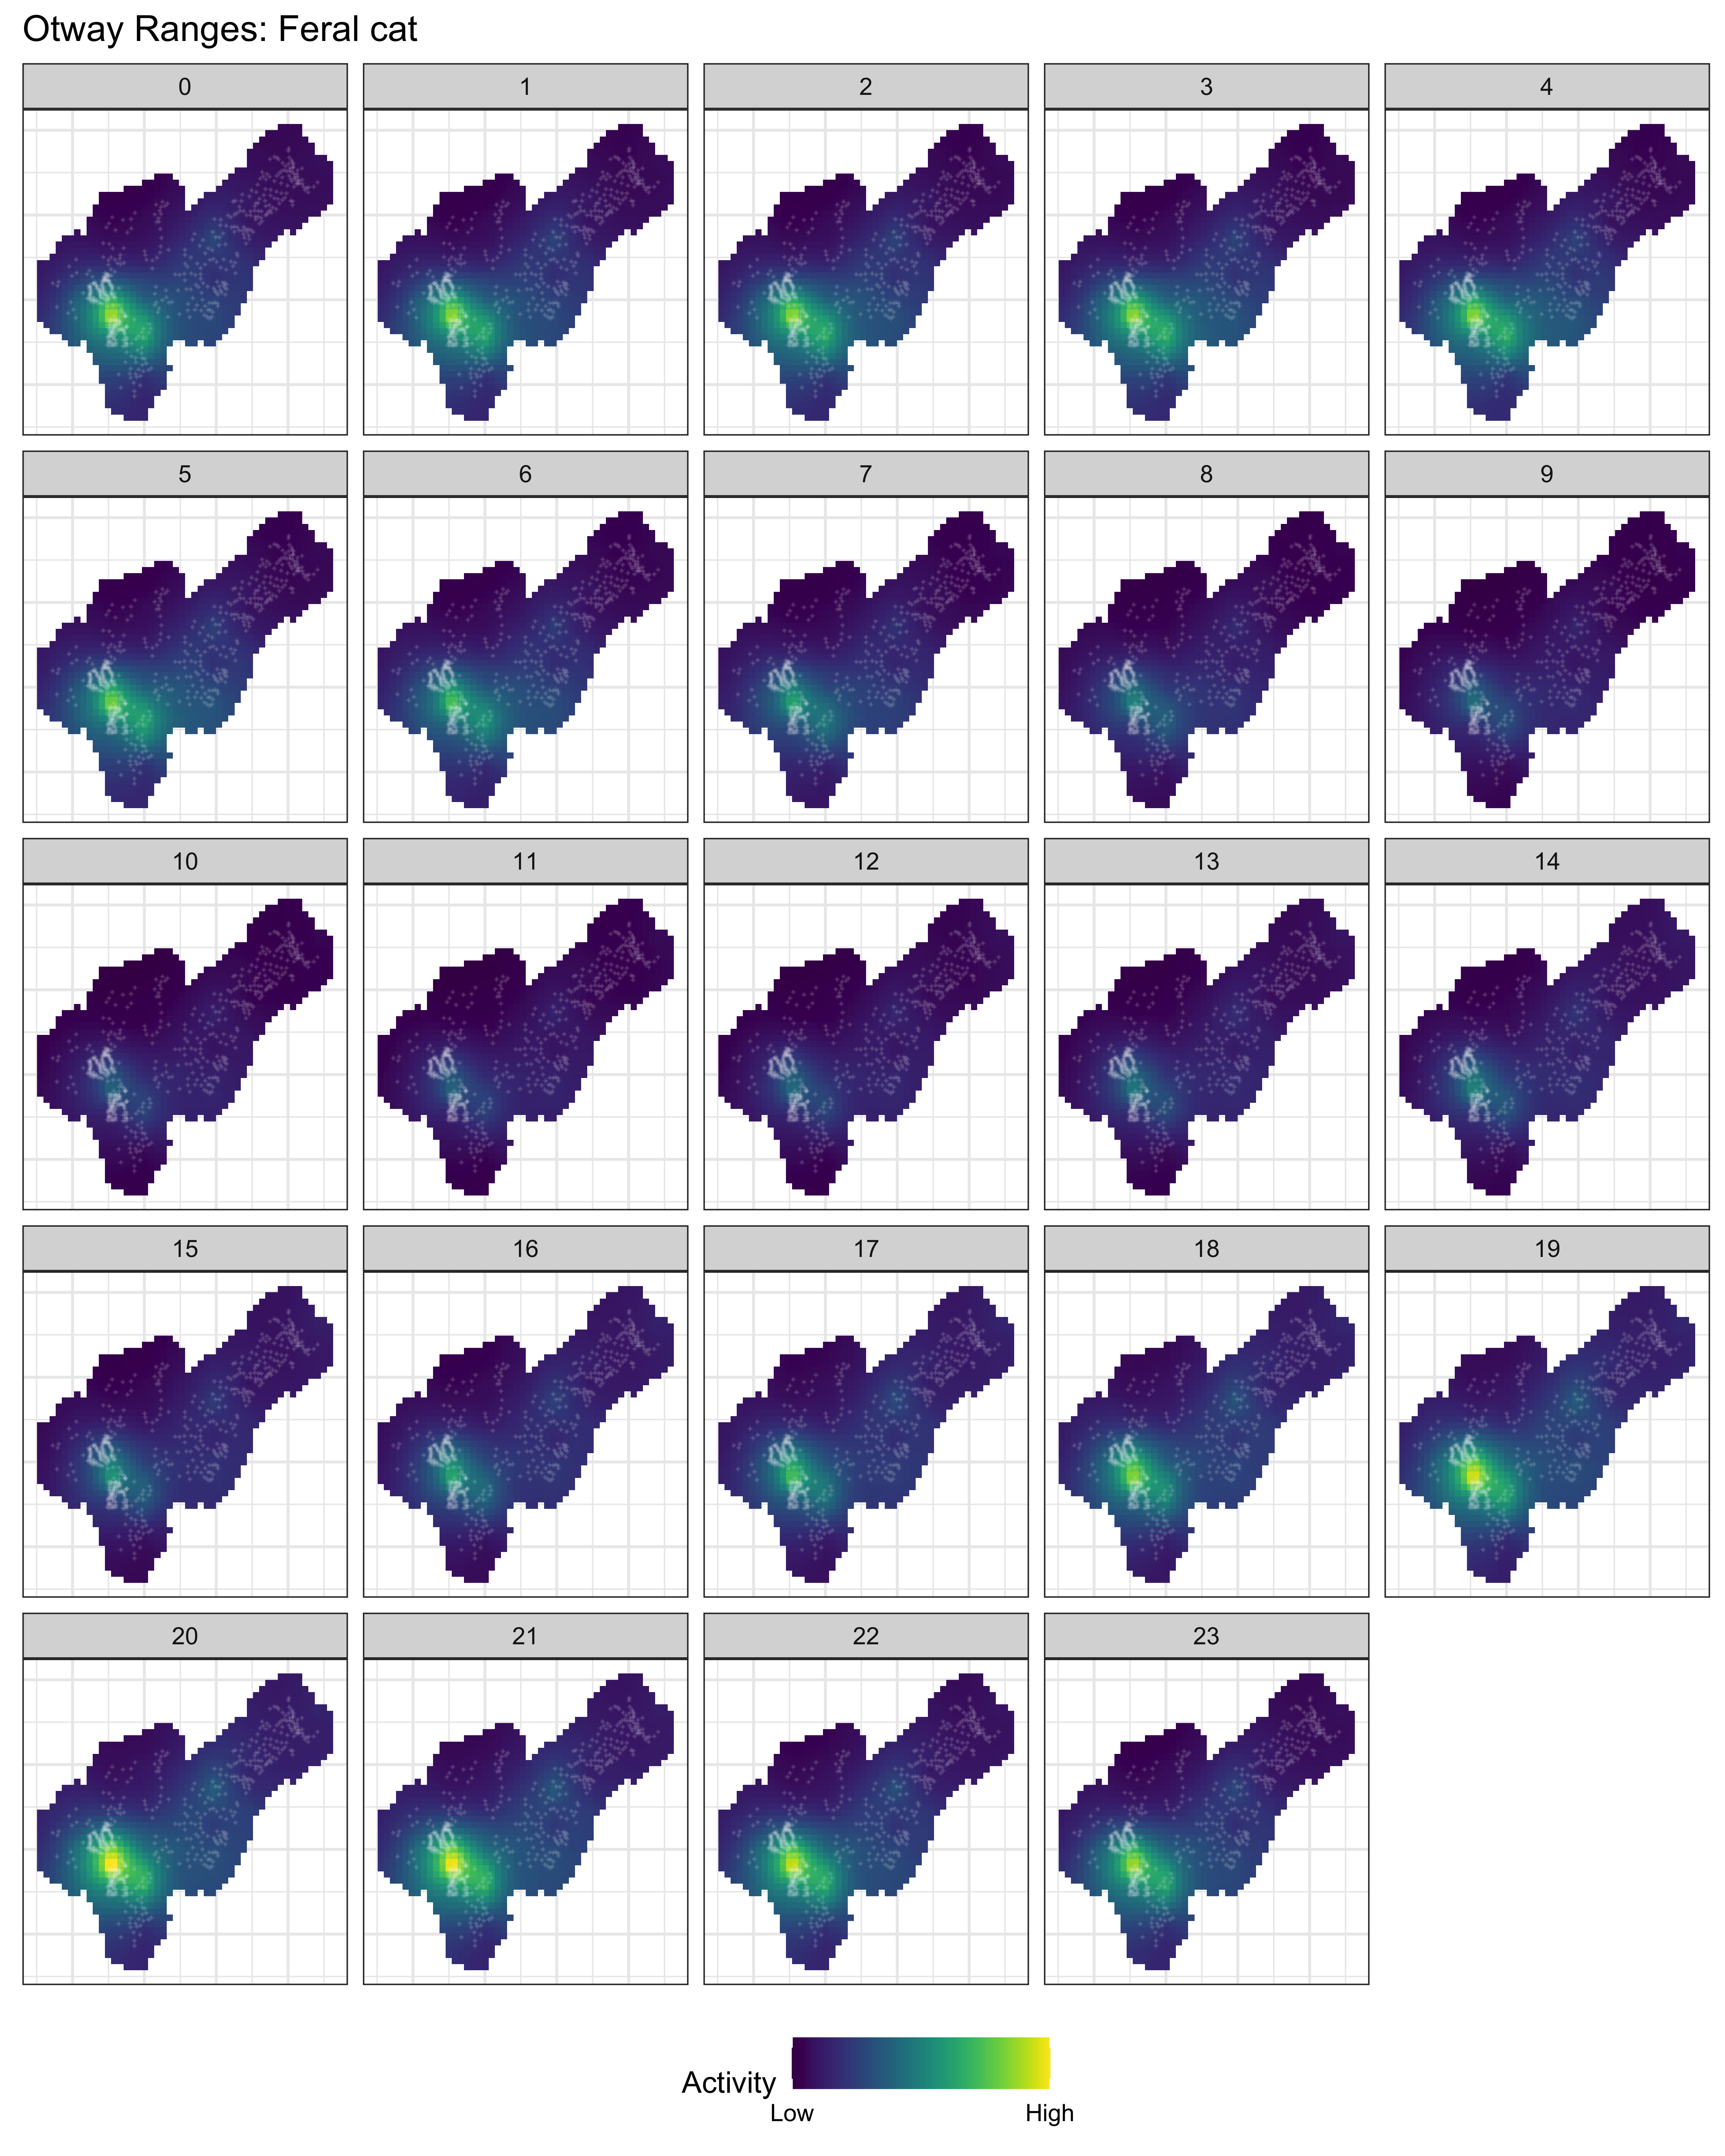
\includegraphics[width=1\linewidth]{figure/spte_facet_o_cat} 

}

\caption{Overall spatial activity of feral cats \textit{Felis catus} for each hour of the day (0 - 23) in the Otway Ranges, Australia (model 1). White crosses depict unique camera-trap sites}\label{fig:diel-space-o-cat}
\end{figure}
\end{mainmatter}
\end{document}
